% !TEX program = pdflatex
% !TEX encoding = UTF-8 Unicode

% TFG basado en la plantilla de la clase `scrbook` del paquete
% KOMA-script para la elaboración de un TFG siguiendo las
% directrices del la comisión del Grado en Matemáticas de
% la Universidad de Granada.

% Autor de la plantilla: Francisco Torralbo Torralbo
% miércoles, 29 de abril de 2020

% Autor de la memoria: Blanca Cano Camarero

%\documentclass{scrbook}
\documentclass[twoside]{scrbook}
\KOMAoptions{%
  fontsize=10pt,        % Tamaño de fuente
  paper=a4,             % Tamaño del papel
  headings=normal,      % Tamaño de letra para los títulos: small, normal, big
  % parskip=half,         % Espacio entre párrafos: full (una línea) o half (media línea)
  headsepline=false,    % Una linea separa la cabecera del texto
  cleardoublepage=empty,% No imprime cabecera ni pie en páginas en blanco
  chapterprefix=false,  % No antepone el texto "capítulo" antes del número
  appendixprefix=false,	% No antepone el texto "Apéndice" antes de la letra
  listof=totoc,		    	% Añade a la tabla de contenidos la lista de tablas y figuras
  index=totoc,			    % Añade a la talba de contenidos una entrada para el índice
  bibliography=totoc,	  % Añade a la tabla de contenidos una entrada para bibliografía
  BCOR=5mm,           % Reserva margen interior para la encuadernación.
                        % El valor dependerá el tipo de encuadernado y del grosor del libro.
  DIV=10,             % Cálcula el diseño de página según ciertos
                        % parámetros. Al aumentar el número aumentamos el ancho de texto y disminuimos el ancho del margen. Una opción de 14 producirá márgenes estrechos y texto ancho.
}


% INFORMACIÓN PARA LA VERSIÓN IMPRESA
% Si el documento ha de ser impreso en papel de tamaño a4 pero el tamaño del documento (elegido en \KOMAoptions con la ocpión paper) no es a4 descomentar la línea que carga el paquete `crop` más abajo. El paquete crop se encargará de centrar el documento en un a4 e imprimir unas guías de corte. El procedimiento completo para imprenta sería el siguiente:
% 0. Determinar, según el tipo de encuadernación del documento, el ancho reservado para el proceso de encuadernación (preguntar en la imprenta), es decir, la anchura del área del papel que se pierde durante el proceso de encuadernación. Fijar la varibale BCOR de \KOMAoptions a dicho valor.
% 1. Descomentar la siguiente línea e imprimir una única página con las guías de corte
% 2. Cambiar la opción `cross` por `cam` (o `off`) en el paquete crop y volver a compilar. Imprimir el documento (las guías de corte impresas no inferfieren con el texto).
% 3. Usar la página con las guías impresas en el punto 1 para cortar todas las páginas.

% \usepackage[a4, odd, center, pdflatex, cross]{crop} % Permite imprimir el documento en un a4 (si el tamaño es más pequeño) mostrando unas guías de corte. Útil para imprenta.

% VERSIÓN ELECTRÓNICA PARA TABLETA
% Las opciones siguientes seleccionan un tamaño de impresión similar a una tableta de 9 pulgadas con márgenes estrechos. Útil para producir una versión en pdf para ser leída en una tableta en lugar de impresa.
% Para que la portada quede centrada correctamente hay que editar el
% archivo `portada.tex` y eliminar el entorno `addmargin`

% \KOMAoptions{fontsize=10pt, paper=19.7104cm:14.7828cm, twoside=false, BCOR=0cm, DIV=14}

% ---------------------------------------------------------------------
%	PAQUETES
% ---------------------------------------------------------------------

% CODIFICACIÓN E IDIOMA
% ---------------------------------------------------------------------
\usepackage[utf8]{inputenc} 			    % Codificación de caracteres

% Selección del idioma: cargamos por defecto inglés y español (aunque este último es el idioma por defecto para el documento). Cuando queramos cambiar de idioma escribiremos:
% \selectlanguage{english} o \selectlanguage{spanish}

\usepackage[english, spanish, es-nodecimaldot, es-noindentfirst, es-tabla]{babel}

% Opciones cargadas para el paquete babel:
  % es-nodecimaldot: No cambia el punto decimal por una coma en modo matemático.
  % es-noindentfirst: No sangra los párrafos tras los títulos.
  % es-tabla: cambia el título del entorno `table` de "Cuadro" a "Tabla"

% Otras opciones del paquete spanish-babel:
  \unaccentedoperators % Desactiva los acentos en los operadores matemáticso (p.e. \lim, \max, ...). Eliminar esta opción si queremos que vayan acentuados

% MATEMÁTICAS
% ---------------------------------------------------------------------
\usepackage{amsmath, amsthm, amssymb} % Paquetes matemáticas
\usepackage{mathtools}                % Añade mejoras a amsmath
\mathtoolsset{showonlyrefs=true}      % sólo se numeran las ecuaciones que se usan
\usepackage[mathscr]{eucal} 					% Proporciona el comando \mathscr para
                                      % fuentes de tipo manuscrito en modo matemático sin sobreescribir el comando \mathcal

% TIPOGRAFÍA
% ---------------------------------------------------------------------
% El paquete microtype mejora la tipografía del documento.
\usepackage[activate={true,nocompatibility},final,tracking=true,kerning=true,spacing=true,factor=1100,stretch=10,shrink=10]{microtype}

% Las tipografías elegidas para el documento son las siguientes
% Normal font: 			URW Palladio typeface.
% Sans-serif font: 	Iwona
% Monospace font: 	Inconsolata
% Consultar http://www.tug.dk/FontCatalogue/ para seleccionar otra tipografía.
% Es conveniente elegir aquellas que tienen soporte matemático.
\usepackage[T1]{fontenc}
\usepackage[sc, osf]{mathpazo} \linespread{1.05}
\usepackage[scaled=.95,type1]{cabin} % sans serif in style of Gill Sans
\usepackage{inconsolata}
% \renewcommand{\sfdefault}{iwona}


% Selecciona el tipo de fuente para los títulos (capítulo, sección, subsección) del documento.
\setkomafont{disposition}{\sffamily\bfseries}

% Cambia el ancho de la cita. Al inicio de un capítulo podemos usar el comando \dictum[autor]{cita} para añadir una cita famosa de un autor.
\renewcommand{\dictumwidth}{0.45\textwidth}

\recalctypearea % Necesario tras definir la tipografía a usar.

% TABLAS, GRÁFICOS Y LISTADOS DE CÓDIGO
% ---------------------------------------------------------------------
\usepackage{booktabs}
% \renewcommand{\arraystretch}{1.5} % Aumenta el espacio vertical entre las filas de un entorno tabular

\usepackage{xcolor, graphicx}
% Carpeta donde buscar los archivos de imagen por defecto
\graphicspath{{img/}}

% IMAGEN DE LA PORTADA
% Existen varias opciones para la imagen de fondo de la portada del TFG. Todas ellas tienen en logotipo de la universidad de Granada en la cabecera. Las opciones son las siguientes:
% 1. portada-ugr y portada-ugr-color: diseño con marca de agua basada en el logo de la UGR (en escala de grises y color).
% 2. portada-ugr-sencilla y portada-ugr-sencilla-color: portada únicamente con el logotipo de la UGR en la cabecera.
\usepackage{eso-pic}
\newcommand\BackgroundPic{%
	\put(0,0){%
		\parbox[b][\paperheight]{\paperwidth}{%
			\vfill
			\centering
      % Indicar la imagen de fondo en el siguiente comando
			
\includegraphics[width=\paperwidth,height=\paperheight,%
			keepaspectratio]{portada/portada-ugr-sencilla-color}%
			\vfill
}}}

\usepackage{listings} % Para la inclusión de trozos de código

% CABECERAS
% ---------------------------------------------------------------------
% Si queremos modificar las cabeceras del documento podemos usar el paquete
% `scrlayer-scrpage` de KOMA-Script. Consultar la documentación al respecto.
% \usepackage[automark]{scrlayer-scrpage}

% VARIOS
% ---------------------------------------------------------------------

%\usepackage{showkeys}	% Muestra las etiquetas del documento. Útil para revisar las referencias cruzadas.

% ÍNDICE
% Para generar el índice hay que compilar el documento con MakeIndex. Generalmente los editores se encargan de ello automáticamente.
% ----------------------------------------------------------------------
% \index{} para añadir un elemento
% \index{main!sub} para añadir un elementos "sub" bajo la categoría "main".
% \index{termino|textbf} para dar formato al número de página (negrita).
% \index{termino|see{termino relacionado}} para crear una referencia cruzada

% Ejemplo: \index{espacio homogéneo}, \index{superficie!mínima}, \index{esfera|see{espacio homogéneo}}
\usepackage{makeidx}
%\usepackage{showidx} % Muestra en el margen del documento las entradas añadidas al índice. Útil para revisar el documento. Si está activo el índice no se genera
\makeindex

% ---------------------------------------------------------------------
% COMANDOS Y ENTORNOS
% ---------------------------------------------------------------------
% Cargamos un archivo externo donde hemos incluido todos los comandos
% propios que vamos a usar en el documento.
% DEFINICIÓN DE COMANDOS Y ENTORNOS

% CONJUNTOS DE NÚMEROS

  \newcommand{\N}{\mathbb{N}}     % Naturales
  \newcommand{\R}{\mathbb{R}}     % Reales
  \newcommand{\Z}{\mathbb{Z}}     % Enteros
  \newcommand{\Q}{\mathbb{Q}}     % Racionales
  \newcommand{\C}{\mathbb{C}}     % Complejos

% Otros espacios 
\newcommand{\D}{\mathcal{D}} % Conjunto de datos de entrenamiento

  %%%%%%%%% Mis comandos %%%%%%%%%
% Para escribir código y pseudo código  
\usepackage{minted}
\usemintedstyle{friendly}
\definecolor{sutilGreen}{rgb}{0.850, 0.996, 0.807} % para el fondo del código
\definecolor{sutilBackground}{rgb}{0.933, 0.905, 0.866}
\newminted{code}{
  frame=single,
  framesep=10pt,
  baselinestretch=1.2,
  bgcolor=sutilBackground, 
  %linenos 
}
\newminted{example}{frame=single,
  framesep=10pt,
  baselinestretch=1.2,
  %bgcolor=sutilBackground, 
  %linenos
}
\usepackage{algorithmic}
% Para la definición de redes neuronales de una sola capa 
\newcommand{\Hu}{\mathcal{H}(X,Y)}  % Espacio de las redes neuronales

% Notas en el margen
\usepackage{sidenotes}
  \newcommand{\afines}{\mathcal{A}(\R^d)}
  \newcommand{\pmc}{\mathcal{H}_G(\R^d,\R)}%{\sum ^r (G)}  % Red neurona una capa una salida
  \newcommand{\pmcg}{ \sum \prod^d (G)} % Generalización red neuronal
  \newcommand{\fC}{\mathcal{C}(\R^d)} %conjunto de funciones continuas en R^r -> R
  \newcommand{\fM}{\mathcal{M}(\R^d)} % Conjunto funiones medibles
  \newcommand{\rrnn}{ \mathcal{H}(\R^d,\R)} % Red neuronal  sin subíndice
  \newcommand{\rrnng}{ \sum \prod^d (\psi)} % Red neuronal  generalizado
  \newcommand{\dist}{\rho_{\mu}}     % Distancia de una medida
  \newcommand{\dlp}{\rho_{p}} % Distancia de los espacios Lp
  % Múltiples salidas 
  \newcommand{\fCC}{\mathcal{C}(\R^d ,\R^s)}
  \newcommand{\fMM}{\mathcal{M}(\R^d , \R^s)}
  \newcommand{\rrnnmc}{ \mathcal{H}(\R^d,\R^s)} 
  \newcommand{\rrnnsmn}{ \mathcal{H}_n(\R^d,\R^s)} % Red neuronal salida múltiple con n neuronas
  \newcommand{\rrnngmc}{ \sum \prod^{d,s} (\psi)} 
  %%%%%%%%% Mis comandos %%%%%%%%%5
\usepackage{sidenotes} % Notas en el margen
\newcommand{\margenimagen}{
  \newgeometry{
      left=2.5cm, % Margen izquierdo
    right=5cm, % Margen derecho
    bottom=2.5cm % Margen inferior}
  }
}
\usepackage{caption}
\usepackage{subcaption}

% TEOREMAS Y ENTORNOS ASOCIADOS

  % \newtheorem{theore<m}{Theorem}[chapter]
  \newtheorem*{teorema*}{Teorema}
  \newtheorem{teorema}{Teorema}[chapter]
  \newtheorem{proposicion}{Proposición}[chapter]
  \newtheorem{lema}{Lema}[chapter]
  \newtheorem{corolario}{Corolario}[chapter]

    \theoremstyle{definition}
  \newtheorem{definicion}{Definición}[chapter]
  \newtheorem{ejemplo}{Ejemplo}[chapter]

    \theoremstyle{remark}
  \newtheorem{observacion}{Observación}[chapter]


\DeclareMathOperator{\sign}{signo}
\usepackage[inline]{enumitem}
\usepackage{mathtools}
\usepackage[spanish,onelanguage,linesnumbered,ruled,vlined]{algorithm2e}
\usepackage{listingsutf8}
\lstset{language=Python,
        literate=
          {ó}{{\'o}}1
          {í}{{\'i}}1
          {á}{{\'a}}1
          {ú}{{\'u}}1
          {é}{{\'e}}1
          {ñ}{{\v{n}}}1
}
\usepackage{tocloft}
\setlength{\cftfignumwidth}{2.55em}
\DeclareMathOperator*{\argmin}{arg\,min}

\SetKwRepeat{Struct}{struct \{}{\}}%

% Para las notas del margen 
%Nota los colores seleccionados han sido creados con una paleta inclusiva
% https://palett.es/6a94a8-013e3b-7eb645-31d331-26f27d
\definecolor{darkRed}{rgb}{0.2,1,0.7}%{ 0.149, 0.99, 0.49}%{1,0.1,0.1}
\definecolor{dark_green}{rgb}{0, 0.24, 0.23} %{0.2, 0.7, 0.2}
\definecolor{blue}{rgb}{0.61, 0.98, 0.759} % sobreeescribimos el azul
\newcommand{\smallMarginSize}{1.8cm}
\newcommand{\bigMarginSize}{3cm}
\newcommand{\maginLetterSize}{\scriptsize}%{\footnotesize} %{\scriptsize}%

% Para los iconos 
\usepackage{fontawesome}
% Alias aclaraciones 
% dark_green
\newcommand{\iconoAclaraciones}{\faQuestionCircleO $\quad$} %\faQuestionCircleO
% blue
\newcommand{\iconoProfundizar}{\faSearch  $\quad$}
\newcommand{\iconoClave}{\faLightbulbO  $\quad$} % \faLightbulbO %\faKey

% Contenido original 
\usepackage{lipsum}
\usepackage[%
linewidth=5pt,
outerlinecolor=red,
outerlinewidth=5pt,
innerlinewidth=1pt,
outerlinecolor=red,
roundcorner=5pt
%middlelinecolor= yellow,
middlelinewidth=0.4pt,
%roundcorner=1pt,
topline = false,
rightline = false,
leftline = false,
bottomline = false,
rightmargin=0pt,
skipabove=7pt,
skipbelow=7pt,
leftmargin=-1cm,
backgroundcolor=black!7,
%innerleftmargin=1cm,
%innerrightmargin=0pt,
%innertopmargin=0pt,
%innerbottommargin=0pt,
frametitlebackgroundcolor=yellow!100,
]{mdframed}
 
\newenvironment{aportacionOriginal}
  {\mdfsetup{
    frametitle=\textcolor{white}{\Large Aportación original}
    %frametitle={\colorbox{black!7}{ \textcolor{white}{\Large Aportación original}}},
    %frametitleaboveskip=-\ht\strutbox,
    %frametitlealignment=\center
    }
  \begin{mdframed}%
  }
  {\end{mdframed}}

  % ancho imágenes en tabla
  \newcommand{\coeficienteAncho}{.3}

% Paquetes para citas
\usepackage{csquotes}
\let\oldenquote\enquote
\renewcommand{\enquote}[1]{{\itshape\oldenquote{#1}}}
\usepackage{epigraph} %este es para las que salen a la derecha




% --------------------------------------------------------------------
% INFORMACIÓN DEL TFG Y EL AUTOR
% --------------------------------------------------------------------
\usepackage{xspace} % Para problemas de espaciado al definir comandos

\newcommand{\miTitulo}{Optimización de redes neuronales\xspace}
\newcommand{\miNombre}{Blanca Cano Camarero\xspace}
\newcommand{\miGrado}{Doble Grado en Ingeniería Informática y Matemáticas}
\newcommand{\miFacultad}{Escuela Técnica Superior de Ingenierías Informática y de Telecomunicación \\ Facultad de Ciencias}
\newcommand{\miUniversidad}{Universidad de Granada}
% Añadir tantos tutores como sea necesario separando cada uno de ellos
% mediante el comando `\\\medskip` y una línea en blanco
\newcommand{\miTutor}{
  Juan Julián Merelo Guervós\\ \emph{Arquitectura y tecnología de computadores}
  \\\medskip

  Francisco Javier Meri de la Maza\\ \emph{Análisis matemático}
}
\newcommand{\miCurso}{2021-2022\xspace}

% HYPERREFERENCES
% --------------------------------------------------------------------
\usepackage{xurl}
\usepackage[pagebackref]{hyperref}
% Opciones para el paquete hyperref
%----------------------------------

\hypersetup{%
  % hidelinks,            % Enlaces sin color ni borde. El borde no se imprime
  linkbordercolor=0.8 0 0,
  citebordercolor=0 0.8 0,
  citebordercolor=0 0.8 0,
  colorlinks = true,            % Color en texto de los enlaces. Comentar esta línea o cambiar `true` por `false` para imprimir el documento.
  linkcolor = [rgb]{0.5, 0, 0}, % Color de los enlaces internos
  urlcolor = [rgb]{0, 0, 0.5},  % Color de los hipervínculos
  citecolor = [rgb]{0, 0.5, 0}, % Color de las referencias bibliográficas
	pdftitle={\miTitulo},%
	pdfauthor={\textcopyright\ \miNombre, \miFacultad, \miUniversidad},%
  pdfsubject={Trabajo de fin de Grado},%
	pdfkeywords={},%
	pdfcreator={pdfLaTeX},%
}

% Redefinición del estilo para mostrar las referencias cruzadas en la bibliografía.
\renewcommand*{\backref}[1]{}
\renewcommand*{\backrefalt}[4]{{\footnotesize [%
    \ifcase #1 No citado%
    \or Citado en pág.~#2%
    \else Citado en págs. #2%
    \fi%
]}}

% Etiquetas en español para el comando \autoref
\def\chapterautorefname{Capítulo}
\def\appendixautorefname{Apéndice}
\def\sectionautorefname{Sección}
\def\subsectionautorefname{Subsección}
\def\figureautorefname{Fig.}
\def\tableautorefname{Tabla}

\def\teoremaautorefname{Teorema}
\def\proposicionautorefname{Proposición}
\def\lemaautorefname{Lema}
\def\corolarioautorefname{Corolario}
\def\definicionautorefname{Def.}
\def\observacionautorefname{Observación}
\def\ejemploautorefname{E.j.}

% Pone automáticamente un parántesis para las ecuaciones
\def\equationautorefname~#1\null{Ec.~(#1)\null}

% Extra
\def\algorithmautorefname{Algoritmo}


\begin{document}

% --------------------------------------------------------------------
% FRONTMATTER
% -------------------------------------------------------------------
%\frontmatter % Desactiva la numeración de capítulos y usa numeración romana para las páginas

% \pagestyle{plain} % No imprime cabeceras

% !TeX root = ../libro.tex
% !TeX encoding = utf8

%*******************************************************
% Titlepage
%*******************************************************
\begin{titlepage}
  \AddToShipoutPicture*{\BackgroundPic}
  \phantomsection
  \pdfbookmark[1]{Título}{title}

  % Para que el título esté centrado en la página.
  % Los valores numéricos deberán elegirse de acuerdo con el diseño de
  % página (sobre todo si se cambia la opción BCOR o DIV).
  \begin{addmargin}[2.575cm]{0cm}
  \begin{flushleft}
    \Large
    \hfill\vfil

    \large{\textsf{\miFacultad}}
    \vfill

    {\large\textsc\miGrado} \vfill


    {\large\textsc{trabajo de fin de grado}}

    \vspace*{0.5cm}

    \begingroup
    \centering
    \Huge{\miTitulo}
    \endgroup

    \vfill\vfill\vfill\vfill

    \textsf{\normalsize{Presentado por:}}\\
    {\normalsize\textrm{\miNombre}}
    \bigskip

    \textsf{\normalsize{Tutores:}}\\
    {\normalsize\rmfamily \miTutor}

    \bigskip
    \textsf{\normalsize{Curso académico \miCurso}}
  \end{flushleft}
  \end{addmargin}

\end{titlepage}
\cleardoublepage
\endinput

% !TeX root = ../libro.tex
% !TeX encoding = utf8

%*******************************************************
% Little Dirty Titlepage
%*******************************************************

\thispagestyle{empty}

\begin{center}
  \large

  \vspace*{\stretch{1}}

  \begingroup
  \huge{\miTitulo} \\ \bigskip
  \endgroup

  \textrm{\miNombre}

  \vspace{\stretch{5}}

\end{center}

\newpage
\thispagestyle{empty}

\hfill

\vfill

\noindent\miNombre \textit{\miTitulo}.

\noindent Trabajo de fin de Grado. Curso académico \miCurso.
\\
\\
\begin{minipage}[t]{0.25\textwidth}
  \flushleft
  \textbf{Responsables de tutorización}
\end{minipage}
\begin{minipage}[t]{0.45\textwidth}
  \flushleft
  \miTutor
\end{minipage}
\begin{minipage}[t]{0.30\textwidth}
  \flushright
  \miGrado
  \medskip

  \miFacultad
  \medskip

  \miUniversidad
\end{minipage}
\begin{flushleft}
\end{flushleft}

\endinput

% !TeX root = ../libro.tex
% !TeX encoding = utf8
%
%*******************************************************
% Declaración de originalidad
%*******************************************************

\thispagestyle{empty}

\hfill\vfill

\textsc{Declaración de originalidad}\\\bigskip

Dña. \miNombre \\\medskip

Declaro explícitamente que el trabajo presentado como Trabajo de Fin de Grado (TFG), correspondiente al curso académico \miCurso, es original, entendida esta, en el sentido de que no ha utilizado para la elaboración del trabajo fuentes sin citarlas debidamente.
\medskip

En Granada a \today
\begin{flushleft}
Fdo: \miNombre

\end{flushleft}

\vfill

\endinput

% !TeX root = ../libro.tex
% !TeX encoding = utf8

%*******************************************************
% Agradecimientos
%*******************************************************

\chapter*{Agradecimientos}

Agradezco a 
\endinput

% !TeX root = ../libro.tex
% !TeX encoding = utf8
%
%*******************************************************
% Resumen
%*******************************************************

% \manualmark
% \markboth{\textsc{Introducción}}{\textsc{Introducción}}

\chapter*{Resumen}\label{ch:resumen}
%\addcontentsline{toc}{chapter}{Resumen}

Existe en la actualidad un desequilibrio entre resultados empíricos 
y teóricos de redes neuronales llegando incluso a contradicción
 (como se comenta en la introducción del capítulo 
 \ref{chapter:Introduction-neuronal-networks}), será por tanto
nuestro primer objetivo construir una teoría sólida
que de cabida a 
 optimizaciones de fundamento teórico; 
una revisión y
 purga de cualquier artificio existente sobre 
 redes neuronales carente de fundamento matemático. 

Como resultado de ello se ha creado e implementado 
un nuevo modelo de red neuronal así como sus 
métodos de aprendizaje y evaluación. 
Además se ha propuesto un criterio de selección de 
funciones de activación y un algoritmo de 
inicialización de pesos que mejora los ya existentes. Todos los resultados han conducido a la creación de 
la biblioteca \textit{OptimizedNeuralNetwork.jl}, que contiene la implementación de nuestros modelos y métodos optimizados. 


La estructura de la memoria es la siguiente: 

\begin{itemize}
    \item \textbf{Capítulo \ref{ch00:methodology}: Descripción de la metodología seguida.} Se ha organizado el proyecto de acorde a una filosofía de desarrollo ágil, basada en la metodología de personas, historias de usuario, hitos y test. Tal método ha conducido e hilado desde el comienzo tanto el desarrollo teórico como el técnico a la par que  salvaguardaba la corrección de cada paso. 
    \item \textbf{Capítulo \ref{chapter:Introduction-neuronal-networks}: Descripción del problema de aprendizaje.} Se introduce las características y tipo de problemas del aprendizaje automático. Además se clarifica cuáles tratan de resolver las redes neuronales. 
    \item \textbf{Capítulo \ref{ch03:teoria-aproximar}: Teoría de la aproximación.} Se muestran los problemas y virtudes que presenta un enfoque clásico  de teoría de la aproximación frente a problemas de aprendizaje. En pos de solventar tales impedimentos,  
    se sitúa esta teoría como el germen de 
    las redes neuronales.
    Concretamente se desarrolla la teoría necesaria hasta demostrar el teorema de \textit{Stone-Weierstrass} y se explicarán las trabas que presentan este tipo de aproximaciones. 
    \item \textbf{Capítulo \ref{chapter4:redes-neuronales-aproximador-universal}: Introducción de las redes neuronales como aproximadores universales.} Se presenta nuestra propuesta de modelo de red neuronal y se compara con los modelos actuales. Se demuestra que nuestra definición actúa como un aproximador universal a cualquier función medible basándonos en el artículo 
    \textit{Multilayer Feedforward Networks are Universal Approximators} (\cite{HORNIK1989359}). Además se demuestran unas serie de resultados sobre cómo es la convergencia en problema de regresión y clasificación. Finalemnte se plantea si en la práctica las redes neuronales 
    verdaderamente son aproximadores universales.
    \item \textbf{Capítulo \ref{chapter:construir-redes-neuronales}: Diseño y construcción de las redes neuronales.} Se describe la implementación de las redes neuronales; esto nos permitirá una comparación  
    más profunda de nuestro modelo frente a los usuales y que nos servirá como justificación del modelo obtenido. Producto de ello son dos resultados originales sobre el sesgo y dominio de la imagen. 
    Una vez determinado el modelo concreto se
    han diseñado un algoritmo de aprendizaje, basado en \textit{Backpropagation} y otro de evaluación de redes neuronales. Además se han comparado los resultados de nuestro modelado con los utilizado usualmente. 
    \item \textbf{Capítulo \ref{funciones-activacion-democraticas-mas-demoscraticas}: Democratización de las funciones de activación.} Se pretende en este capítulo determinar qué funciones de activación son más convenientes que otras, es decir, con cuál se podría tener un menor coste computacional. 
    Para esto, no se ha tenido sólo en cuenta el coste computacional de evaluar cada función; puesto que la imagen de una función de activación repercute 
    en el número de neuronas necesarias para estar por debajo de cierto error, se ha establecido una serie de teoremas propio que determina qué funciones de activación tendrán los mismos resultados.  Gracias a tales resultados se han 
    podido agrupar a las funciones de activación y 
    para cada clase se ha tratado de determinar por medio del test de hipótesis de Wilcoxon cuál es la más rápida, resultando con esto que sin perder precisión se ha reducido el costo y tiempo en evaluación y entrenamiento de las redes neuronal. 
    
    \item \textbf{Capítulo \ref{section:inicializar_pesos}: Algoritmo de inicialización de pesos.} Se propone un algoritmo original de inicialización de los pesos de una red neuronal a 
    partir de un subconjunto de datos de la muestra. Al ser la solución de partida mejor, con este método se pretende reducir el tiempo y coste de aprendizaje de técnicas iterativas, tales como \textit{Backpropagation}.  
    
    En este capítulo se muestran además los 
    requisitos técnicos de la implementación de la biblioteca \textit{OptimizedNeuralNetwork.jl}, 
    ya que para medir la bondad del algoritmo es 
    necesario implementar todas las funcionalidades al completo. Además se han añadido en estas 
    secciones ejemplo de uso de la biblioteca. 
    \item \textbf{Capítulo \ref{ch08:genetic-selection}: Selección genética de las funciones de activación.} El uso de distintas funciones de activación presenta un 
    potencial en cuanto a reducir el error fijado un cierto número de neuronas, sin embargo esto 
    aumenta el espacio de búsqueda y por tanto la complejidad. Es aquí donde nuestro modelo 
    propuesto de red neuronal palía la situación, 
    ya que frente a los modelos convencionales, el nuestro es invariante a la posición de las 
    funciones de activación de las neuronas, lo cual
     reduce el espacio de búsqueda.  
\end{itemize}

\paragraph{PALABRAS CLAVE:}
\begin{itemize*}[label=,itemsep=1em,itemjoin=\hspace{1em}]
  \item redes neuronales
  \item optimización 
  \item funciones de activación 
  \item inicialización de pesos
\end{itemize*}

\endinput

% !TeX root = ../libro.tex
% !TeX encoding = utf8
%
%*******************************************************
% Summary
%*******************************************************

\selectlanguage{english}
\chapter*{Summary}\label{ch:summary}
%\addcontentsline{toc}{chapter}{Summar}

Nowadays experimental research in Neural Networks is more advanced than theoretical
results. 
From this we aim to establish a solid mathematical theory so as to optimize the current neural network models. 


As a result of our study, we have proposed a novel neural 
network model, and adapted and optimized
evaluation and learning methods to it. 
Moreover, we have discovered some theorems that prove the 
equivalence among some activation functions, and hence propose a new
 algorithm to initialize weights of neural networks. Thanks to the
first result, we obtain a criteria to choose the most 
suitable activation function to maintain accuracy and reduce computational costs.
 Thanks to the second one, we might accelerate 
learning convergence methods.

In addition, the models, methods and algorithms have been 
implemented in Julia, resulting in the \textit{OptimizedNeuralNetwork.jl} library. 

All the theory development, designs, decisions and results are 
written in this memory, which have the following structure: 
\begin{itemize}
 \item \textbf{Chapter \ref{ch00:methodology}: Description of the methodology followed.} We have organized our project according to an agile philosophy  based on personas methodology, user stories, milestones and tests. This method has conducted and linked mathematical and technical results and implementations, giving them coherence and validation methods. 

 \item \textbf{Chapter \ref{chapter:Introduction-neuronal-networks}: Description of the learning problem.} We defined the characteristic and type of machine learning problems. We will focus on supervised learning ones. 

 \item \textbf{Chapter \ref{ch03:teoria-aproximar}:  Approximation theory.} In order to establish a solid theory, we will start our work trying to solve machine learning problems by traditional approximation methods.  The main result we prove is the Stone Weierstrass's theorem. As a conclusion of this chapter we will achieve knowledge of the virtues and faults of traditional methods and understanding the necessity of new methods and structures such as neural networks. 

 \item \textbf{Chapter \ref{chapter4:redes-neuronales-aproximador-universal}: Neural networks are universal approximators.}  In this chapter we introduce our neural 
 network model and compare it with the conventional ones. In order to show it is well 
 defined, we will prove the universal convergence of our model to any measurable 
 function. In addition, we will give some results about how our model solves 
 classification and regression problems as its number of neurons rises. Finally, we 
 will argue if all of those math results can actually solve real life problems. The 
 idea behind the debate is the computability representation of real numbers. 

 \item \textbf{Chapter  \ref{chapter:construir-redes-neuronales}: The design and implementation of neural networks.} We will carefully  describe the design and 
 implementation of our model of neural network. Thanks to that we will obtain some 
 mathematical results about bias and classification function. This will be useful to 
 compare our model with the conventional ones and justify 
our selection. Moreover, we will explain, justify and design  learning and evaluation 
methods to our model. These methods are optimized versions of Forward Propagation and 
Backpropagation. 

\item \textbf{Chapter \ref{funciones-activacion-democraticas-mas-demoscraticas}: Democratization of activation functions.} 
We will explain in this chapter if there are better activation functions. In this 
direction we will prove two original results which show that there are families of 
activation functions that with the same conditions will solve problems with the same 
accuracy. As a result, if we compare the computational cost of the members of those 
families and choose the faster one, we will obtain a method to optimize evaluation and 
learning of neural networks without loss of accuracy. We have used the Wilcoxon 
signed-rank test as a statistical hypothesis test so as to give a rigorous study of 
our criteria. 

\item \textbf{Chapter \ref{section:inicializar_pesos}: Weight initializing algorithm.} 
Since the Backpropagation and other iterative  methods are sensitive to the initial 
value of a neural network, we will show an original method to initialize its weights 
from training data. This process not only will produce a better initial step but also 
has lower computational cost than Backpropagation.  To test the potential of this 
method we will use the Wilcoxon signed-rank test again and also, from the experiment's 
requirements we will design and create our OptimizedNeuralNetwork.jl library. In this chapter we 
will also explain every decision done during the design and implementation of the 
library in order to be as efficient as possible.	

\item \textbf{Chapter \ref{ch08:genetic-selection}: Use of genetic algorithm in the selection of activation function.} 
In this chapter we will explain a future work. Given a fixed number of neurons, the 
selection of its activation function may be crucial to reduce the train and test 
error.  However, adding more free params to the search space increases its complexity 
and at same time the cost of finding a solution.  Nevertheless, the result obtained at 
chapter \ref{funciones-activacion-democraticas-mas-demoscraticas} and a property of our neural model will reduce the space complexity.

\item \textbf{Chapter \ref{ch09:conclusion}: Conclusions.}
\end{itemize} 

\paragraph{KEYWORDS:}
\begin{itemize*}[label=,itemsep=1em,itemjoin=\hspace{1em}]
  \item neural networks
  \item optimization
  \item activation functions
  \item weights initializing
  \item machine learning library
\end{itemize*}

% Al finalizar el resumen en inglés, volvemos a seleccionar el idioma español para el documento
\selectlanguage{spanish}
\endinput

%\include{preliminares/dedicatoria}                % Opcional
% !TeX root = ../libro.tex
% !TeX encoding = utf8

%*******************************************************
% Table of Contents
%*******************************************************
\phantomsection
\pdfbookmark[0]{\contentsname}{toc}

\setcounter{tocdepth}{2} % <-- 2 includes up to subsections in the ToC
\setcounter{secnumdepth}{3} % <-- 3 numbers up to subsubsections

% \manualmark
% \markboth{\textsc{\contentsname}}{\textsc{\contentsname}}
\tableofcontents 

%*******************************************************
% List of Figures and of the Tables
%*******************************************************

    % *******************************************************
    %  List of Figures
    % *******************************************************    
    \phantomsection 
    \listoffigures

    %*******************************************************
    % List of Tables
    %*******************************************************
    \phantomsection 
    \listoftables
    
    %*******************************************************
    % List of Algorithms
    %*******************************************************
    \phantomsection
    \listofalgorithms
    
    %*******************************************************
    % List of Listings
    % The package \usepackage{listings} is needed
    %*******************************************************      
	  % \phantomsection 
    % \renewcommand{\lstlistlistingname}{Listados de código}
    % \lstlistoflistings 

\cleardoublepage

            % Opcional

% \pagestyle{scrheadings} % A partir de ahora sí imprime cabeceras
% TODO
%% !TeX root = ../../tfg.tex
% !TeX encoding = utf8
%
%*******************************************************
% Introducción artículo MFNAUA
%*******************************************************
\section{Las redes neuronales son aproximadores universales}  

Tras las definición \ref{sec:redes-neuronales-intro-una-capa} de red neuronal expuesta,
es pertinente la pregunta si tal estructura será 
capaz de aproximar con éxito una función genérica desconocida.   

Aunque las redes neuronales multicapa ya se venían aplicando con anterioridad, 
véase por ejemplo los usos expuestos durante la primera conferencia
internacional de redes neuronales de \cite{4307059} de 1987, 
no fue hasta 1989 que se descubrió formalmente su alcance.
 Tal delimitación se propuso en el artículo 
\textbf{Multilayer Feedforward Networks are Universal Approximators} \cite{HORNIK1989359}
 escrito por Kurt Hornik, Maxwell Stinchcombe y Halber White enunciando: 

\begin{teorema}\textbf{Las redes \textit{feedforward} multicapa son una clase de aproximadores universales } \label{teo:MFNAUA}
    \\
    Una red neuronal \textit{feedforward} multicapa estándar con tan solo una capa oculta y con una función de activación cualquiera es capaz de aproximar cualquier 
    función Borel medible  con dominios y codominios de dimensión finita (no necesariamente iguales) y con el nivel de precisión que se desee siempre y cuando 
    se utilicen suficientes neuronas. En este sentido las redes \textit{feedforward} multicapa son una clase de aproximadores universales.

\end{teorema}

En las secciones siguientes, con el fin de alcanzar una
 comprensión profunda de las redes neuronales,
trataremos de desgranar y profundizar en el artículo y su 
demostración. Primero precisaremos o introduciremos conceptos elementales 
sobre redes neuronales \ref{ch:articulo:sec:defincionesPrimeras}, después 
demostraremos el teorema en el caso real 
\ref{teo:TeoremaConvergenciaRealEnCompactosDefinicionesEsenciales} e iremos refinando y generalizando los resultados hasta probar
el resultado enunciado \ref{teo:MFNAUA} para una capa oculta.

 % Nota margen de denso
 \setlength{\marginparwidth}{\bigMarginSize}
 \marginpar{\maginLetterSize
     \iconoAclaraciones \textcolor{dark_green}{ 
         \textbf{Idea intuitiva conjunto denso.}
     }
     Si $S$ es denso en $T$, 
     se está está diciendo que \textbf{los elementos de $S$ son capaces de aproximar cualquier elemento de $T$
     con la precisión que se desee}. 
 }

 
El esquema general será: 

\begin{align*}
    \rrnn 
        \xRightarrow[]{\ref{teo:2_4_rrnn_densas_M}}  
    \rrnng 
        \xRightarrow[]{\ref{teorema:2_3_uniformemente_denso_compactos}}
    \pmcg
        \xRightarrow[]{\ref{teo:TeoremaConvergenciaRealEnCompactosDefinicionesEsenciales}}     
    \fC    
        \xRightarrow[]{\ref{teo:2_2_denso_función_continua}} 
    \fM.
\end{align*}

   

\begin{itemize}
    \item Las redes neuronales que nosotros hemos modelizado son densas en un espacio más general que hemos denominado \textit{Anillo de aproximación de redes neuronales}
    generado a partir de una función de activación $\psi$. 
    \item Que a su vez es denso en el \textit{Anillo de aproximación de redes neuronales}
    generado a partir de una función medible $G$. 
    \item El espacio \textit{Anillo de aproximación de redes neuronales} es denso en el de las funciones continuas.
    \item Las funciones continuas son densas en el espacio de funciones medibles. 
\end{itemize}

Si quisiéramos situar en este esquema a otras definiciones de redes neuronales las situaríamos entre  nuestro modelo y el espacio \textit{Anillo de aproximación de redes neuronales}; en  el capítulo \ref{chapter:construir-redes-neuronales} se probará tal resultado y analizarán los beneficios de basarnos en un modelo más simple. 



%

% --------------------------------------------------------------------
% MAINMATTER
% --------------------------------------------------------------------
%\mainmatter % activa la numeración de capítulos, resetea la numeración de las páginas y usa números arábigos
\setpartpreamble[c][0.75\linewidth]{
	%\bigskip % Deja un espacio vertical en la parte superiọ-r
  
}
%%%%%%%%%%%%%%%%%%%%%%%%%%%%%%%%%%
%% Comentarios previos 
%%%%%%%%%%%%%%%%%%%%%%%%%%%%%%%%%%
% Convenio colores notas
%%%%%%%%%%%%%%%%%%%%%%%%%%%%%%%%%%

\section*{Comentario previo}

Se pretende con este documento presentar un  trabajo de fin de grado de Ingeniería Informática y Matemáticas y que cualquier miembro del tribunal; 
independientemente de la vertiente a la que pertenezca sea capaz de comprenderlo en su totalidad.  
Para ello se ha acompañado la exposición con notas en los márgenes aclaratorias, que siguen el siguiente código de color y icono: 

\begin{itemize}
    \item  \iconoAclaraciones \textcolor{dark_green}{ Color 1}: Comentarios para 
    aclarar conceptos matemáticos o informáticos ofertar la idea intuitiva que 
    se esconde, donde no se presuponen conocimientos avanzados en 
    la materia. 
    \item  \iconoProfundizar \textcolor{blue}{  Color 2}: Comentarios para una reflexión más profunda o que indique nuevas áreas que explorar. 
    \item  \iconoClave  \textcolor{darkRed}{  Color 3}: Concepto clave y destacable que tendrá un papel fundamental a posteriori.  
\end{itemize}

%Nota los colores seleccionados han sido creados con una paleta inclusiva
% https://palett.es/6a94a8-013e3b-7eb645-31d331-26f27d

%%%%%%%%%%%%%%%%%%%%%%%%%%%%%%%%%%%%%%%%%%%%%%%%%%%%%%%%%%%%%%%%%%%%%%%%%%%
%% Introducción para comenzar la teoría hablando de la filosofía que se va a seguir 
%%
%%%%%%%%%%%%%%%%%%%%%%%%%%%%%%%%%%%%%%%%%%%%%%%%%%%%%%%%%%%%%%%%%%%%%

\chapter*{Introducción}

\section*{Origen}
En nuestros días, el aprendizaje automático es un campo en
continua expansión. Desde procesamiento de imágenes hasta predicciones de
acciones en bolsa, las redes neuronales se van implantando en todos los
campos del conocimiento. \\


A pesar del pragmatismo actual que prevalece en las redes 
neuronales, el concepto de neurona artificial nace en el primer tercio del siglo XX con el artículo  \textit{ Logical calculus of the ideas immanent in nervous activity} \cite{primer-articulo}, como
intento de modelar el pensamiento humano en forma de proceso lógico. Esta
primera etapa de investigación culmina con la invención del perceptrón en
1958 por Frank Rosenblatt con el artículo \textit{The perceptron: a probabilistic model for information storage and organization in the brain} \cite{rosenblatt1958perceptron}. Es importante notar que todas estas investigaciones
tenían un objetivo más allá de la resolución de problemas complejos utilizando
máquinas u ordenadores: comprender el proceso de aprendizaje y cognición del
ser humano.\\

Estos primeros modelos tenían sus carencias y reservas por parte
de la comunidad científica y cuando en 1969 la publicación de la demostración de que
los modelos eran incapaces de resolver problemas lógicos simples (véase \cite{minsky69perceptrons}) hizo que el
campo casi muriera. No fue hasta 1986 con el descubrimiento de un modelo en más complejo,
que se superarían estas limitaciones y que darían lugar a las actuales redes neuronales
\cite{10.5555/104279.104293}.\\

El modelos de 1986, no obstante, usaba un método que sus autores eran incapaces de
relacionar con el mundo de la cognición, suponiendo con esto el 
inicio de la separación de las redes neuronales con el campo de la psicología
y la neurociencia y el inicio del enfoque actual de resolución de problemas.
Estos nuevos descubrimientos, sumados a una mejora en las capacidades
computacionales de los ordenadores y que en 1989 demostrara formalmente su eficacia \cite{HORNIK1989359} provocaron un auge en el interés acerca de
las redes, que perdura hasta hoy.\\


\section*{Descripción del problema,  motivación y objetivos} 
Si bien las redes neuronales abandonaron ya la psicología 
y a pesar de su uso extensivo en la actualidad, es un área incipiente de la 
matemática donde los grandes teoremas aún están por descubrir. 
Ante tal desequilibrio entre resultados empíricos y teóricos,
 será 
nuestro primer objetivo conseguir una revisión y purga de cualquier artificio
 existente sobre redes neuronales carente de fundamento matemático. 
Siendo el fin de esto construir una teoría sólida que de cabida a 
optimizaciones de fundamento teórico.

\section*{Técnicas, áreas matemáticas y fuentes utilizadas}  

El artículo principal que membrana el proyecto es el artículo 
\textit{Multilayer Feedforward Networks are Universal Approximators} \cite{HORNIK1989359}
 escrito por Kurt Hornik, Maxwell Stinchcombe y Halber White. Como pilar a la 
 sección de teoría de aproximación se ha utilizad el manual \textit{The Elements of Real Analysis} \cite{the-elements-of-real-analysis} y finalmente los manuales de referencia seguidos sobre el aprendizaje automático han sido: 
 \textit{Learning From Data} \cite{MostafaLearningFromData} y \textit{Pattern Recognition and Machine Learning} \cite{BishopPaterRecognition}.

 Sobre las técnicas y áreas empleadas pueden consultarse con detalle en la secciones \ref{ch01:Herramientas} y \ref{ch01:asignaturas}.


%Metodología 

% !TeX root = ../../tfg.tex
% !TeX encoding = utf8
%
%*******************************************************
% Introducción artículo MFNAUA
%*******************************************************
\section{Las redes neuronales son aproximadores universales}  

Tras las definición \ref{sec:redes-neuronales-intro-una-capa} de red neuronal expuesta,
es pertinente la pregunta si tal estructura será 
capaz de aproximar con éxito una función genérica desconocida.   

Aunque las redes neuronales multicapa ya se venían aplicando con anterioridad, 
véase por ejemplo los usos expuestos durante la primera conferencia
internacional de redes neuronales de \cite{4307059} de 1987, 
no fue hasta 1989 que se descubrió formalmente su alcance.
 Tal delimitación se propuso en el artículo 
\textbf{Multilayer Feedforward Networks are Universal Approximators} \cite{HORNIK1989359}
 escrito por Kurt Hornik, Maxwell Stinchcombe y Halber White enunciando: 

\begin{teorema}\textbf{Las redes \textit{feedforward} multicapa son una clase de aproximadores universales } \label{teo:MFNAUA}
    \\
    Una red neuronal \textit{feedforward} multicapa estándar con tan solo una capa oculta y con una función de activación cualquiera es capaz de aproximar cualquier 
    función Borel medible  con dominios y codominios de dimensión finita (no necesariamente iguales) y con el nivel de precisión que se desee siempre y cuando 
    se utilicen suficientes neuronas. En este sentido las redes \textit{feedforward} multicapa son una clase de aproximadores universales.

\end{teorema}

En las secciones siguientes, con el fin de alcanzar una
 comprensión profunda de las redes neuronales,
trataremos de desgranar y profundizar en el artículo y su 
demostración. Primero precisaremos o introduciremos conceptos elementales 
sobre redes neuronales \ref{ch:articulo:sec:defincionesPrimeras}, después 
demostraremos el teorema en el caso real 
\ref{teo:TeoremaConvergenciaRealEnCompactosDefinicionesEsenciales} e iremos refinando y generalizando los resultados hasta probar
el resultado enunciado \ref{teo:MFNAUA} para una capa oculta.

 % Nota margen de denso
 \setlength{\marginparwidth}{\bigMarginSize}
 \marginpar{\maginLetterSize
     \iconoAclaraciones \textcolor{dark_green}{ 
         \textbf{Idea intuitiva conjunto denso.}
     }
     Si $S$ es denso en $T$, 
     se está está diciendo que \textbf{los elementos de $S$ son capaces de aproximar cualquier elemento de $T$
     con la precisión que se desee}. 
 }

 
El esquema general será: 

\begin{align*}
    \rrnn 
        \xRightarrow[]{\ref{teo:2_4_rrnn_densas_M}}  
    \rrnng 
        \xRightarrow[]{\ref{teorema:2_3_uniformemente_denso_compactos}}
    \pmcg
        \xRightarrow[]{\ref{teo:TeoremaConvergenciaRealEnCompactosDefinicionesEsenciales}}     
    \fC    
        \xRightarrow[]{\ref{teo:2_2_denso_función_continua}} 
    \fM.
\end{align*}

   

\begin{itemize}
    \item Las redes neuronales que nosotros hemos modelizado son densas en un espacio más general que hemos denominado \textit{Anillo de aproximación de redes neuronales}
    generado a partir de una función de activación $\psi$. 
    \item Que a su vez es denso en el \textit{Anillo de aproximación de redes neuronales}
    generado a partir de una función medible $G$. 
    \item El espacio \textit{Anillo de aproximación de redes neuronales} es denso en el de las funciones continuas.
    \item Las funciones continuas son densas en el espacio de funciones medibles. 
\end{itemize}

Si quisiéramos situar en este esquema a otras definiciones de redes neuronales las situaríamos entre  nuestro modelo y el espacio \textit{Anillo de aproximación de redes neuronales}; en  el capítulo \ref{chapter:construir-redes-neuronales} se probará tal resultado y analizarán los beneficios de basarnos en un modelo más simple. 



%%%%%%%%%%%%%%%%%%%%%%%%%%%%%%%%%%%%%%%%%%%%%%%%%%%%%%%%%%%%%%%%
% Justificación de porqué se ha seleccionado Julia como lenguaje de programación 
%%%%%%%%%%%%%%%%%%%%%%%%%%%%%%%%%%%%%%%%%%%%%%%%%%%%%%%%%%%%%%%%

\section{Herramientas utilizadas}

\subsection{GitHub}
Como servicio externo hemos usado \href{https://github.com}{GitHub}, ya que permite implementar de manera eficaz
 todo el desarrollo ágil: 
desde la planificación, comunicación, test e incluso difusión y acceso a los resultados. 

\subsection{Lenguaje de programación Julia}
Hemos seleccionado como lenguaje de programación \href{https://julialang.org}{Julia} 
por los siguientes motivos (\cite{virtudes-de-julia}): 
\begin{itemize}
    \item Ofrece \textit{benchmarks} 
    muy competitivos\footnote{Véase los resultado expuestos en 
    \url{https://julialang.org/benchmarks/}, 
    web consultada por última vez el 22 de mayo de 2022.},
    al nivel de C.
    \item Variedad de bibliotecas usadas para ciencia de datos que podríamos encontrar 
    en otros lenguajes muy utilizados en el sector como son Python y R. 
    \item Otras características del lenguaje que facilitan 
    la optimización del código como veremos en la sección \ref{ch06:activation-function-implementation}. 
\end{itemize}

\subsection{\textit{Notebooks}}
% Comentario sobre qué es un scripts
\marginpar{\maginLetterSize
    \iconoAclaraciones \textcolor{dark_green}{     
        \textbf{
            Significado del término \textit{script}
        }
    }

    Término para designar un programa relativamente simple y que por lo general
    es interpretado (se va traduciendo y ejecutando línea  a línea).
}

Todos los gráficas que se muestran en la memoria han sido creadas por nosotros. 
Las hemos generado con \textit{scripts} o la mayoría de la veces con 
\href{https://jupyter.org}{\textit{notebooks} de Jupyter}, el motivo de esto ha 
sido el tener una interacción y visualización más cómoda y compacta de los resultados.

El lenguaje utilizado en los \textit{notebooks} ha sido Julia o Python indistintamente,
a conveniencia de cuál ofrecía la función o biblioteca más cómoda para el propósito.  


 
%%%%%%%%%%%%%%%%%%%%%%%%%%%%%%%%%%%%%%%%%%%%%%%%%%%%%%%%
%           Asignaturas del grado relacionadas 
%%%%%%%%%%%%%%%%%%%%%%%%%%%%%%%%%%%%%%%%%%%%%%%%%%%%%%%%

\section{Asignaturas de grado relacionadas con el trabajo }  

\epigraph{El todo es más que la suma de sus partes.
}{\textit{Aristóteles}}
Si bien, es casi imposible enumerar de manera
exhaustiva todas las asignaturas involucradas en este trabajo,
ya que todas han influido en menor o mayor medida en la comprensión 
y formulación de ideas; las principales han
sido: 
\begin{itemize}
    \item \textbf{Análisis Matemático}: todas las asignaturas del departamento de análisis matemático
    han tenido relevancia, ya sea en el modelado de espacios de funciones,
    para probar que las redes neuronales son aproximadores universales
    y para la elaboración de nuestro propios resultados.  
    \item El \textbf{Aprendizaje Automático} y \textbf{Visión por Computador} sientan las bases de lo que son problemas de aprendizaje, 
    tratamiento de los datos y evaluación del error, así como el uso práctico de las redes neuronales. 
    \item \textbf{Estructura de Datos}: diseño e implementación de la modelización de las redes neuronales y 
    sus algoritmos concernientes. 
    \item \textbf{Infraestructura virtual}:la metodología y buenas práctica seguidas han 
    bebido en gran parte de las recursos provenientes de tal asignatura. 
\end{itemize}

En menor medida han tenido también relevancia: 
\begin{itemize}
    \item \textbf{Inferencia Estadística}, la Inferencia Estadística está estrechamente ligada con 
    la ciencia de datos, también ha sido utilizada para los test de hipótesis. 
    \item Otras asignaturas que han intervenido \textbf{Programación Orientada a Objeto} \textbf{Diseño y Desarrollo de Sistemas Informáticos}
    \item Nociones de \textbf{Topología} se han requerido para probar ciertos resultados analíticos. 
    \item \textbf{Álgebra, Métodos Numéricos I, Modelos I y Geometría III} esta agrupación de asignaturas 
    han ayudado a la comprensión  y servido como germen de ideas y relaciones a lo largo de todo el desarrollo de la memoria, 
    por poner algunos ejemplos: la relación entre grafo y una matriz proviene de la asignatura de Modelos, 
    la existencia de funciones cuyo error tiende a infinito de Métodos Numéricos,
    resultados constructivos  que después han podido ser implementados (Álgebra y Métodos Numéricos), algunos resultados propios sobres las funciones de activación (Geometría).
\end{itemize}

% Filosofía a seguir   
%%%%%%%%%%%%%%%%%%%%%%%%%%%%%%%%%%%%%%%%%%%%%%%%%%%%%%%%%%%%%%%%%%%%%%%%%%%%
%% Introducción para comenzar la teoría hablando de la filosofía que se va a seguir 
%%
%%%%%%%%%%%%%%%%%%%%%%%%%%%%%%%%%%%%%%%%%%%%%%%%%%%%%%%%%%%%%%%%%%%%%

\chapter*{Introducción}

\section*{Origen}
En nuestros días, el aprendizaje automático es un campo en
continua expansión. Desde procesamiento de imágenes hasta predicciones de
acciones en bolsa, las redes neuronales se van implantando en todos los
campos del conocimiento. \\


A pesar del pragmatismo actual que prevalece en las redes 
neuronales, el concepto de neurona artificial nace en el primer tercio del siglo XX con el artículo  \textit{ Logical calculus of the ideas immanent in nervous activity} \cite{primer-articulo}, como
intento de modelar el pensamiento humano en forma de proceso lógico. Esta
primera etapa de investigación culmina con la invención del perceptrón en
1958 por Frank Rosenblatt con el artículo \textit{The perceptron: a probabilistic model for information storage and organization in the brain} \cite{rosenblatt1958perceptron}. Es importante notar que todas estas investigaciones
tenían un objetivo más allá de la resolución de problemas complejos utilizando
máquinas u ordenadores: comprender el proceso de aprendizaje y cognición del
ser humano.\\

Estos primeros modelos tenían sus carencias y reservas por parte
de la comunidad científica y cuando en 1969 la publicación de la demostración de que
los modelos eran incapaces de resolver problemas lógicos simples (véase \cite{minsky69perceptrons}) hizo que el
campo casi muriera. No fue hasta 1986 con el descubrimiento de un modelo en más complejo,
que se superarían estas limitaciones y que darían lugar a las actuales redes neuronales
\cite{10.5555/104279.104293}.\\

El modelos de 1986, no obstante, usaba un método que sus autores eran incapaces de
relacionar con el mundo de la cognición, suponiendo con esto el 
inicio de la separación de las redes neuronales con el campo de la psicología
y la neurociencia y el inicio del enfoque actual de resolución de problemas.
Estos nuevos descubrimientos, sumados a una mejora en las capacidades
computacionales de los ordenadores y que en 1989 demostrara formalmente su eficacia \cite{HORNIK1989359} provocaron un auge en el interés acerca de
las redes, que perdura hasta hoy.\\


\section*{Descripción del problema,  motivación y objetivos} 
Si bien las redes neuronales abandonaron ya la psicología 
y a pesar de su uso extensivo en la actualidad, es un área incipiente de la 
matemática donde los grandes teoremas aún están por descubrir. 
Ante tal desequilibrio entre resultados empíricos y teóricos,
 será 
nuestro primer objetivo conseguir una revisión y purga de cualquier artificio
 existente sobre redes neuronales carente de fundamento matemático. 
Siendo el fin de esto construir una teoría sólida que de cabida a 
optimizaciones de fundamento teórico.

\section*{Técnicas, áreas matemáticas y fuentes utilizadas}  

El artículo principal que membrana el proyecto es el artículo 
\textit{Multilayer Feedforward Networks are Universal Approximators} \cite{HORNIK1989359}
 escrito por Kurt Hornik, Maxwell Stinchcombe y Halber White. Como pilar a la 
 sección de teoría de aproximación se ha utilizad el manual \textit{The Elements of Real Analysis} \cite{the-elements-of-real-analysis} y finalmente los manuales de referencia seguidos sobre el aprendizaje automático han sido: 
 \textit{Learning From Data} \cite{MostafaLearningFromData} y \textit{Pattern Recognition and Machine Learning} \cite{BishopPaterRecognition}.

 Sobre las técnicas y áreas empleadas pueden consultarse con detalle en la secciones \ref{ch01:Herramientas} y \ref{ch01:asignaturas}.



% Redes neuronales Definición de la clase de redes neuronales 
% !TeX root = ../../tfg.tex
% !TeX encoding = utf8

\chapter{Introducción a las redes neuronales} 

Toma en la actualidad un papel clave en el desarrollo tecnológico el aprendizaje automático
\cite{importancia-arte-aprendizaje-automatico}, siendo 
las redes neuronales un modelo ampliamente usado en este contexto y por ello 
nuestro objetivo de democratización. 
% TODO ya escribiré en el summary necesario que queremos decir con democratización 
Comenzaremos pues  sentando las bases y 
formalizando 
qué significa 
que una máquina \textit{aprenda}  y cómo puede conseguirse, 
todo ello en la sección \ref{sec:Aprendizaje}.
Continuaremos en \ref{sec:redes-neuronales-intro} 
definiendo las redes neuronales, cómo se construyen y evalúan. 

% !TeX root = ../../tfg.tex
% !TeX encoding = utf8
%
%*******************************************************
% Qué es el aprendizaje automático
%*******************************************************

\section{Concepto de aprendizaje}\label{sec:Aprendizaje}

El término de Aprendizaje Automático 
\cite{hisour} 
fue acuñado en 1959 por Arthur Samuel 
para hacer referencia a los sistemas informáticos que 
pudiesen \textit{aprender} por sí mismos, es decir, mejorar su 
eficacia y rendimiento de forma autónoma a partir de los datos, 
sin que en esas mejoras intervenga un programador.

Fue en 1997 cuando Tom Mitchell propuso una definición 
formal de aprendizaje 
\cite{tom-michell-machine-learning}, 
aproximada a la dada en el libro \textit{Learning from data}
\cite{learning-from-data-1-2}, que expondremos en seguida.

El aprendizaje es un proceso por el cual se estima una dependencia desconocida 
(input-output) o la estructura de un sistema a partir de un número finito de 
observaciones. Se compone de tres elementos principales: 

\begin{itemize}
    \item Un generador o función de distribución de la cual se extraen 
    vectores aleatorios 
    $x \in I \subset \mathbb R^ n$ 
    que dependen de una función de densidad desconocida \footnote{De hecho, encontrar esta función resolvería el problema de aprendizaje}.
    
    \item Un sistema que produce un vector de salida $y$ por cada entrada del vector $x$ a partir del valor fijo $p(y|x)$, que es desconocido también. 
    
    \item Una \textit{learning machine} dependiente de parámetros $w$, que en el caso más general no es  más que un conjunto de funciones abstractas cuyos elementos son de la forma $f(x,w)$.
\end{itemize}



Así pues, el objetivo del aprendizaje automático es encontrar una función que se aproxime a la función de densidad desconocida.

Por lo general la teoría se fundamenta en minimizar el error de estimadores, como el error cuadrático medio, ya que este se trata de un UMVUE  (estimador insesgado de mínima varianza). 

$$ECM = \frac{1}{n} \sum_{i=0} ^n (f(x_i) - y_i)^2,$$

donde $f(x_i)$ representa la predicción y $y_i$ la etiqueta de entrenamiento de $x_i$, es decir, su valor real.

% Componentes del aprendizaje   
\subsection{Componentes del aprendizaje}\label{sub:componentes_aprendizaje}  
A nivel práctico y en nuestro caso, los elementos que consideraremos para el aprendizaje y los cuales 
serán susceptibles de contribuir a la optimización buscada son
(capítulo 1 \cite{MostafaLearningFromData}): 


\begin{itemize}
    \item Espacio muestral $\mathcal X$.  
    \item Una función objetivo ideal y desconocida
     $f: \mathcal X \longrightarrow \mathcal{Y},$ 
     donde  $\mathcal{Y}$ es el conjunto de posibles valores asociados. 
    \item Un conjunto de datos de entrenamiento $\mathcal D$, donde los elementos son pares $(x,y)$ con $x \in  \mathcal X$ y 
    $y \in \mathcal{Y}$ y que representa una observación $f(x)=y.$
    \item Un algoritmo de aprendizaje que consiste en seleccionar una fórmula $g: \mathcal X \longrightarrow \mathcal{Y}$ que aproxime $f$. La fórmula $g$ pertenece 
    a un conjunto $\mathcal H$ de hipótesis. 
\end{itemize}

En nuestro caso $\mathcal{H}$ será el conjunto de todas las posibles redes neuronales y $g$ la red neuronal seleccionada. 


% Tipos de aprendizaje 
\subsection{Tipos de aprendizaje}  

Esta clasificación proviene del artículo \cite{importancia-arte-aprendizaje-automatico},
 del capítulo 1 \cite{MostafaLearningFromData}
 y capítulo 4 pag 179
\cite{BishopPaterRecognition}).

El aprendizaje a partir de los datos trata en esencia de modelizar un patrón, modelo o ley del proceso subyacente a partir de un conjunto finito de muestras.  

En función de ciertas características del conjunto de datos se 
tienen distintos tipos de aprendizaje.  

\subsubsection{Aprendizaje supervisado}
Cuando el conjunto de datos de entrenamiento contiene de manera explícita lo que es una salida correcta respecto a una entrada estamos frente a un caso de \textbf{aprendizaje no supervisado}.   
Este tipo de aprendizaje resuelve tareas de clasificación, donde la salida es discreta 
o de regresión, con una salida continua.
Un ejemplo sería el reconocimiento de dígitos  manuscritos donde cada imagen de un dígito tiene asociado cuál es. 




\subsubsection{Aprendizaje por refuerzo}  
Se trata de un problema de aprendizaje por refuerzo 
cuando conjunto de datos de entrenamiento no explicita la salida, en su lugar contiene posibles salidas junto a la bondad de éstas. 

Pongamos por ejemplo que se quiere enseñar a un sistema a jugar
a las damas; de todo el espacio de jugadas posibles, se conocerían tan solo el resultado de algunas situaciones, por ejemplo en la que uno de los jugadores ha ganado.  


\subsubsection{Aprendizaje no supervisado}  

En este tipo de aprendizaje, los datos de entrenamiento tampoco contienen ninguna información de la salida.
 Tan solo se tienen los datos de entrada. El \textbf{aprendizaje no supervisado} 
 consiste en la tarea de encontrar patrones y estructuras en los datos de entrada, 
 así como de crear una una abstracción de los datos.  Son problemas de \textit{clustering}, asociación, detección de anomalías ...

\subsubsection{Aprendizaje semi supervisado }
Combina tanto datos etiquetados como no etiquetados, 
se utiliza en problemas de clasificación o \textit{clustering}
como por ejemplo en traducción o detección de fraudes.


Las redes neuronales son partícipes en los tres tipos de aprendizaje 
recién mencionados
\cite{8612259}, \cite{DBLP:journals/corr/BakerGNR16}, \cite{10.5555/2955491.2955578}. Sin embargo centraremos nuestro estudio en el caso 
de aprendizaje supervisado. 


\subsection{El gradiente descendente} \label{sec:gradiente-descendente}

(Información tomada de los capítulos uno y dos de \cite{learning-from-data-1-2})
Así pues, una vez concretado el problema y sus elementos 
(\ref{sub:componentes_aprendizaje}) es necesario definir un método con el que aproximar la función ideal $f,$ para ello introduciremos el algoritmo de gradiente descendente.  

El gradiente descendente es un método iterativo de minimización de funciones diferenciables. 

En nuestro caso particular se quiere aproximar la función ideal desconocida $f$ a partir de funciones (redes neuronales) $h_w \in \mathcal{H}$, donde $w \in M(\R)_{m \times n}$ son parámetros que caracterizan a $h_w$.
Para  
Dada también una función de error diferenciable y que no presente puntos de inflexión
$E: M(\R)_{m \times n} \longrightarrow \R,$
se toma una matriz inicial  cualquiera $w_0 \in M(\R)_{m \times n}$ y 
fijado $\eta \in \R^+$. 

Se define la sucesión 
\begin{equation}
    w_{t+1}  = w_t - \eta \nabla E(w_t).
\end{equation}  

Donde $w_n$ es una sucesión cuyos términos convergen a un mínimo local.
\subsubsection*{Observaciones sobre el algoritmo }

\begin{itemize}
    \item El algoritmo solo encuentra óptimos locales con una dependencia crucial del valor de inicio. 
    \item La convergencia no es segura en un tiempo finito y requiere de criterios de parada. 
    \item Si la función es convexa el mínimo será global.
    \item El parámetro $\eta$ puede ser cualquiera y debe de ser fijado o controlado por el diseñador.  
\end{itemize}


\subsection{Comentario de Blanca que deja aquí por guardarlo en algún sitio y que en algún momento debiera de borrar} 

\textcolor{blue}{
Estamos buscando verdaderamente no una función ideal sino 
la clase de equivalencia de las funciones medibles que coincide su grafo en un conjunto numerable de puntos. 
En la práctica nos quedamos con un candidato de esa clase. ¿ Afectar esta forma de ver las cosas?
}



% Teoría de la aproximación 
% !TeX root = ../../tfg.tex
% !TeX encoding = utf8
%%%%
% OBJETIVOS SOBRE EL CAPÍTULO DE TEORÍA DE LA PROXIMACIÓN 
%%%%%%%%

\chapter{Teoría de la aproximación}
 \label{chapter:teoria-aproximar}

 Puesto que queremos fundamentar desde el origen las redes neuronales,
 supongamos que desconociéramos la existencia de éstas
 y nos halláramos frente a un problema de aprendizaje \ref{sec:Aprendizaje}; 
 el enfoque más natural consistiría en abordar el problema 
 haciendo uso de teoría de la aproximación.  
 ¿Somos capaces de aproximar una función a partir de sus puntos?






% !TeX root = ../../tfg.tex
% !TeX encoding = utf8
%
%*******************************************************
% Polinomios de Bernstein
%*******************************************************

\section{Polinomios de Bernstein}\label{ch:Bernstein}  

%% Resumen capítulo 
En esta sección introduciremos los polinomios de Bernstein   
que, vistos como una serie, nos asegurarán una convergencia uniforme a cualquier 
función continua en un compacto y serán esenciales para nuestra prueba del teorema de Stone-Weierstrass, 
las pruebas se basan en el manual \cite{the-elements-of-real-analysis}.  

    % Nota margen de compacto
    \reversemarginpar 
    \setlength{\marginparwidth}{\smallMarginSize}
    \marginpar{\maginLetterSize
        \iconoAclaraciones \textcolor{dark_green}{ 
            \textbf{Idea intuitiva compacto}
        }

        Un compacto es un conjunto que se puede cambiar por un subconjunto finito cometiendo un error prefijado. 
    
    }
    \normalmarginpar
    \setlength{\marginparwidth}{\bigMarginSize}
    


% Nota margen sobre Idea intuitiva convergencia uniforme
\marginpar{\maginLetterSize
\iconoAclaraciones \textcolor{dark_green}{     
\textbf{¿Qué es la convergencia uniforme?}}.
    Cuando se hable de \textbf{convergencia} nos referiremos 
    a encontrar un elemento que \textbf{aproxime todo lo bien que queramos};
    es decir, fijado cualquier error podemos encontrar un elemento 
    que lo aproxime cometiendo un error menor. 
    
    Tengamos presente que en el contexto de funciones
    el error se puede medir evaluando la imagen de cada punto del dominio; entonces  
    con \textbf{uniforme} lo que se dice es que independientemente del error que se busque, 
    se puede encontrar una función que \textbf{para todos los puntos del dominio
     aproxima al objetivo
    por debajo de ese error}.  
}

Comenzaremos recordando el Teorema del Binomio de Newton. 

%% Teorema Binomio de Newton
\begin{teorema}[Binomio de Newton]
    Cualquier potencia de un binomio $x+y$ con $x,y \in \R$,  puede ser expandido en una suma de la forma
    \[
        (x+y)^n = \sum_{k=0}^n \binom{n}{k} x^{k}y^{n-k}. 
    \]
\end{teorema} 

% Nota margen sobre Idea intuitiva sobre porqué se está procediendo de esta manera 
\marginpar{\maginLetterSize
\iconoAclaraciones \textcolor{dark_green}{     
\textbf{¿Con qué idea se está avanzando?}}.

    Nuestro objetivo es ser capaces de aproximar una función 
    a partir de una muestra de sus preimágenes e imágenes. 
    Comenzaremos probando primero que dada una función continua, podemos
    aproximarla a partir de una muestra concreta. 
    Por eso se está tratando de reescribir la función en 
    términos de cierto conjunto de sus imágenes. 
}
%%% Idea intuitiva y desigualdad 
Tomando ahora para esta igualdad $x \in \R, y= 1-x$ se tiene que 

\begin{equation}\label{eq:uno_igual_binomio}
    1 = (x+ (1-x))^n = \sum_{k=0}^n \binom{n}{k} x^{k} (1-x)^{n-k}.
\end{equation}

Dada cualquier función continua $f: I \longrightarrow \R$ podríamos multiplicar la ecuación 
\eqref{eq:uno_igual_binomio} por $f(x)$ resultando 

\begin{equation}\label{eq:f_igual_binomio}
    f(x) = \sum_{k=0}^n f(x) \binom{n}{k} x^{k} (1-x)^{n-k}.
\end{equation} 

Y tomando como dominio $I=[0,1]$ de $f: I \longrightarrow \R$,
 nos encontramos
frente a una ecuación muy sugerente para introducir $B_n(x)$, el \textit{Polinomio n-ésimo  de Bernstein}. 
El cual pretende  aproximar la función $f$ a través de los puntos $\frac{k}{n}$ con $n \in \N$ fijo
y $k \in \{0,...,n \}.$

\begin{definicion}[Polinomios de Bernstein] \label{def:Bernstein}
    Dada cierta función $f: [0,1] \rightarrow \R$, se define el n-ésimo polinomio de Bernstein para $f$ como 

    $$B_n(x) = B_n(x;f)=\sum_ {k=0}^{n} \left( f \left( \frac{k}{n} \right) \binom{n}{k} x^k (1-x)^{n-k} \right).$$

\end{definicion}

Faltaría por ver si efectivamente nuestro polinomio construido
 \textit{aproxima lo suficientemente bien} a la $f$ originaria. 
Basándonos en la igualdad \eqref{eq:f_igual_binomio} y 
la diferencia entre $f(x)$ y $B_n(x)$ se concluye que

%\begin{equation}
%    f(x)-B_n(x) = \sum_{k=0}^n \left(f(x) - f \left( \frac{k}{n} \right)\right)
%    \binom{n}{k} x^{k} (1-x)^{n-k}
%\end{equation} 

%Tomando valor absoluto resulta 
\begin{equation} \label{eq:eq:Bernstein_diferencia}
    |f(x)-B_n(x)| \leq \sum_{k=0}^n \left|f(x) - f \left( \frac{k}{n} \right)\right|
    \binom{n}{k} x^{k} (1-x)^{n-k}
\end{equation} 

Ante tal igualdad la intuición ya nos
hace pensar que sea convergente al aumentar el tamaño de la partición.
 En efecto, en nuestro siguiente teorema, nos cercioraremos de que \ref{def:Bernstein}
 es uniformemente convergente a $f$ en un compacto. 

Para la demostración será necesario el siguiente resultado técnico: 
% Lema ecuación que se usa para una de las demostraciones del lema de Bernstein
\begin{lema}
    Se desea probar la siguiente igualdad 

    \begin{equation} \label{eq:binomio_segunda_suma}
        \frac{1}{n} x (1-x)= \sum_{k=0}^{n}  \left( x-\frac{k}{n} \right)^2  \binom{n}{k} x^{k} (1-x)^{n-k}.
     \end{equation}
\end{lema}
% Nota margen sobre el lema
\marginpar{\maginLetterSize
    \iconoAclaraciones \textcolor{dark_green}{     
        \textbf{
            Resultado técnico. 
        }
    }
    La demostración del lema \ref{eq:binomio_segunda_suma}
    se ha incluido para que todo resultado esté fundamentado, solo se utiliza para establecer una cota necesaria en una desigualdad del teorema \ref{teo:aproximacion_bernstein}.  
     
}
\begin{proof}

    %%% propiedades coeficientes binomial 

    Tengamos ahora presente las siguientes igualdades 
    \begin{equation} \label{eq:binomio_menos_uno}
        \binom{n-1}{k-1} = \frac{(n-1)!}{(k-1)! (n-1-(k-1))!} = \frac{k}{n} \binom{n}{k}
    \end{equation}
    \begin{equation} \label{eq:binomio_menos_dos}
        \binom{n-2}{k-2} = \frac{(n-2)!}{(k-2)! (n-2-(k-2))!} = \frac{k(k-1)}{n(n-1)} \binom{n}{k}
    \end{equation}

    Partiendo de la igualdad \eqref{eq:uno_igual_binomio}:
    \begin{equation}
        1 = (x+ (1-x))^n = \sum_{k=0}^n \binom{n}{k} x^{k} (1-x)^{n-k}.
    \end{equation}

    Reemplazamos la $n$ por $n-1$ y la $k$ por $j$ y tenemos 
    \begin{equation}
        1 = \sum_{j=0}^{n-1} \binom{n-1}{j} x^{j} (1-x)^{(n-1)-j}.
    \end{equation}
    Multiplicamos por $x$ y aplicamos la igualdad \eqref{eq:binomio_menos_uno} resultando 

    \begin{equation}
        x = \sum_{j=0}^{n-1} \frac{j+1}{n} \binom{n}{j+1} x^{j+1} (1-x)^{n-(j+1)}.
    \end{equation}

    Renombramos $k= j+1$, por lo que resulta
    \begin{equation}
        x = \sum_{k=1}^{n} \frac{k}{n} \binom{n}{k} x^{k} (1-x)^{n-k}.
    \end{equation}

    Como el término con $k=0$ es nulo podemos añadirlo a la sumatoria
    
    \begin{equation} \label{eq:desarrollo_binomio_uno}
        x = \sum_{k=0}^{n} \frac{k}{n} \binom{n}{k} x^{k} (1-x)^{n-k}.
    \end{equation}
    %------------------ caso 2, no te confundas --------------------
    Haremos ahora un razonamiento similar sustituyendo $n$ por $n-2$.
    Partiendo de \eqref{eq:uno_igual_binomio} se tiene que 
    \begin{equation}
        1 = (x+ (1-x))^n = \sum_{k=0}^n \binom{n}{k} x^{k} (1-x)^{n-k}.
    \end{equation}
    Reemplazamos la $n$ por $n-2$ y la $k$ por $j$ y tenemos 
    \begin{equation}
        1 = \sum_{j=0}^{n-2} \binom{n-2}{j} x^{j} (1-x)^{(n-2)-j}.
    \end{equation}
    Multiplicamos por $x^2$ y aplicamos la igualdad \eqref{eq:binomio_menos_dos} resultando 
    \begin{equation}
        x^2 = \sum_{j=0}^{n-2} \frac{(j+2)(j+1)}{n(n-1)} \binom{n}{j+2} x^{j+2} (1-x)^{n-(j+2)}.
    \end{equation}
    Renombramos $k= j+2$, por lo que resulta
    \begin{equation}
        x^2 = \sum_{k=2}^{n} \frac{k(k-1)}{n(n-1)} \binom{n}{k} x^{k} (1-x)^{n-k}.
    \end{equation}
    Como con los términos $k=0$ y $k=1$ se anula, podemos añadir dichos índices sin modificar la suma 
    \begin{equation}
        x^2 = \sum_{k=0}^{n} \frac{k(k-1)}{n(n-1)} \binom{n}{k} x^{k} (1-x)^{n-k}.
    \end{equation}
    Podemos reescribir la ecuación resultando: 
    \begin{equation}\label{eq:desarrollo_binomio_dos}
      (n^2 - n)  x^2 = \sum_{k=0}^{n} (k^2 - k) \binom{n}{k} x^{k} (1-x)^{n-k}.
    \end{equation}
    
    
%--------------- fin de las igualdades del binomio de Newton 

Sumando las dos expresiones que hemos obtenido
 \eqref{eq:desarrollo_binomio_uno} y \eqref{eq:desarrollo_binomio_dos}
 resulta: 
 \begin{equation} 
    (n^2 - n)  x^2 + nx= \sum_{k=0}^{n} ((k^2 - k)+k) \binom{n}{k} x^{k} (1-x)^{n-k}.
  \end{equation}
  Dividimos todo entre $n$. 
  \begin{equation} \label{eq:binomio_tras_suma}
    (1 - \frac{1}{n})  x^2 + \frac{1}{n}x= \sum_{k=0}^{n} \left( \frac{k}{n} \right)^2 \binom{n}{k} x^{k} (1-x)^{n-k}.
  \end{equation}
  A continuación sumamos a la igualdad \eqref{eq:binomio_tras_suma} la ecuación \eqref{eq:uno_igual_binomio} multiplicada por $x^2$ y la ecuación \eqref{eq:desarrollo_binomio_uno}
  multiplicada por $-2x$ resultando: 
  \begin{equation} 
    \left(1 - \frac{1}{n} + 1 -2 \right)  x^2 + \frac{1}{n}x= \sum_{k=0}^{n} \left( \left( \frac{k}{n} \right)^2 + x^2 -2x \right) \binom{n}{k} x^{k} (1-x)^{n-k}.
  \end{equation}
  Sacando factor común en el miembro de la izquierda y escribiendo como un cuadrado el factor de la derecha,  resulta la igualdad \ref{eq:binomio_segunda_suma} que buscábamos
  \begin{equation} 
     \frac{1}{n} x (1-x)= \sum_{k=0}^{n}  \left( x-\frac{k}{n} \right)^2  \binom{n}{k} x^{k} (1-x)^{n-k}.
  \end{equation}
\end{proof}

\begin{teorema}[Teorema de aproximación de Bernstein]\label{teo:aproximacion_bernstein}

    Sea $f$ una función continua de un intervalo $I = [0,1]$ con imágenes en los reales. 
    La sucesión de polinomios de Bernstein
    \ref{def:Bernstein} converge uniformemente a $f$ en $I.$
    
\end{teorema}
Recordaremos antes la definición de convergencia uniforme: 

\begin{definicion}[Convergencia uniforme para funciones reales]

    Dado $E$ un conjunto y $\{f_n\}_{n \in \N}$ una sucesión de funciones de $E$
    a los reales, se dice 
    que dicha sucesión converge uniformemente si para cualquier $\varepsilon > 0$ existe un número natural $m$ tal que 
    para todo $x   \in E$ y cualquier natural $n$ que cumpla $n \geq m$ se tiene que 

    \begin{equation*}
        |f_n(x) - f(x) | < \varepsilon
    \end{equation*}
    
\end{definicion}

% Demostración de la convergencia de los polinomios de Bernstein
Comencemos pues con la demostración del teorema \ref{teo:aproximacion_bernstein}.
\begin{proof}
    
    Para cualquier $\varepsilon > 0$ queremos probar que existe un $m_\varepsilon  \in \N$ tal que para 
    todo $x \in I$ e $n \geq m_\varepsilon$  se tiene que 
    $|f(x) - B_n(x)| < \varepsilon$.
    
     Para ello por estar $f$ definida en un intervalo, 
    se tienen dos consecuencias claves: 
    \begin{enumerate}
        \item Está acotada, supongamos por $M \in \R$, esto es $|f(x)| \leq M$. \label{consecuencia:M}
        \item En virtud del teorema de Heine-Cantor $f$ es uniformemente continua, es decir, por estar $f$ definida en un compacto,  para cualquier $\varepsilon >0$ existirá un $\delta_\varepsilon$
        tal que para cualesquiera $x,y \in I$ que cumplan $|x-y| < \delta_\varepsilon$ entonces $|f(x)-f(y)| < \varepsilon$. \label{consecuencia:delta}
    \end{enumerate}
    %% Cota 2M para  cada sumando
    En virtud de la consecuencia \refeq{consecuencia:M}. 
    Dado $N \in  \N$ fijo pero arbitrario, para cualquier $k \in \{1, ..., N\}$ se tiene que
    $\frac{k}{N} \in I$ y tomando $x \in I$ podemos acotar por la desigualdad triangular

    $$\left|f(x)- f\left( \frac{k}{N} \right) \right| \leq |f(x)| + \left|f \left( \frac{k}{N}\right) \right|\leq 2M.$$  
    Por (\refeq{eq:eq:Bernstein_diferencia}) 
    \begin{equation*}
        |f(x)-B_n(x)| 
        \leq
        \sum_{k=0}^n \left|f(x) - f \left( \frac{k}{n} \right)\right| 
     \binom{n}{k} x^{k} (1-x)^{n-k}.
    \end{equation*}

    Puesto que tenemos que $f$ acotada por $M$ y es uniformemente continua, para valores de $k$ tales que $\frac{k}{n}$ 
    esté próxima a $x$, tal término de la sumatoria será pequeño por la continuidad de $f$ en $x$. Por otro lado
    si está lo suficientemente alejado, tan solo podremos acotar tal término por $2M$.  

    Para $\varepsilon > 0$ y para $\delta_\varepsilon$ de la definición de continuidad uniforme de $f$ 
    podemos encontrar un 
    \begin{equation} \label{eq:cota-de-la-n}
        n \geq \sup \left\{ (\delta_\varepsilon)^{-4}, \frac{M^2}{ \varepsilon^2}\right\}.
    \end{equation}
    Separaremos pues nuestra sumatoria en los siguientes dos conjuntos. 
    % Conjunto de los que son menores
    \begin{equation}
        \mathcal{A}_{n x} = \left\{ k \text{ tales que } k \in \{0,..., n\} \text{ y  } \left|x - \frac{k}{n}\right| < n^{\frac{-1}{4}} \leq \delta_\varepsilon \right\},
    \end{equation}
    % Conjunto de los que son mayores
    \begin{equation}
        \mathcal{B}_{n x} = \{0,..., n\} 
        \setminus
        \mathcal{A}_{n x}. 
    \end{equation}

     Para los elementos de $\mathcal{A}_{n x}$ se obtiene la siguiente estimación: 

     \begin{equation*}
        \begin{split}
        \sum_{k \in \mathcal{A}_{n x} } \left|f(x) - f \left( \frac{k}{n} \right)\right|
     \binom{n}{k} x^{k} (1-x)^{n-k}
     \leq 
     \sum_{k \in \mathcal{A}_{n x} } \varepsilon \binom{n}{k} x^{k} (1-x)^{n-k} 
     =  \\
      = \varepsilon \sum_{k \in \mathcal{A}_{n x} }  \binom{n}{k} x^{k} (1-x)^{n-k} 
     \leq 
     \varepsilon \sum_{k = 0} ^ n  \binom{n}{k} x^{k} (1-x)^{n-k} = 
     \varepsilon
        \end{split}
    \end{equation*}

    Para los elementos de $ \mathcal{B}_{n x}$ se tiene que 
    $(x - \frac{k}{n})^2 \geq  n^{\frac{-1}{2}}$.
    Usando esto y la consecuencia \refeq{consecuencia:M} podemos escribir:
    
    \begin{align*}
        &\sum_{k \in \mathcal{B}_{n x} } \left|f(x) - f \left( \frac{k}{n} \right)\right|
     \binom{n}{k} x^{k} (1-x)^{n-k}
     \\
     & 
     \leq 
      \sum_{k \in \mathcal{B}_{n x}} 2M 
    \binom{n}{k} x^{k} (1-x)^{n-k}
    \\ 
    & 
    = 2M \sum_{k \in \mathcal{B}_{n x}} 
    % multiplicamos y dividimos por diferencias 
    \frac{
        \left(x- \frac{k}{n}\right)^2
    }{
        \left(x- \frac{k}{n}\right)^2
    }
    \binom{n}{k} x^{k} (1-x)^{n-k}
    \\
    &
    % cota de la fracción introducida 
    % y más sumandos
    \leq 2M 
    \sqrt{n}
    \sum_{k \in \mathcal{B}_{n x}} 
    \left(x- \frac{k}{n}\right)^2
    \binom{n}{k} x^{k} (1-x)^{n-k}
    \\
    & % cota del lema
    \leq
    2M \sqrt{n}
    \left(
        \frac{1}{n} x(1-x)
    \right)
    \leq 
    \frac{M}{2 \sqrt{n}}.
    \end{align*}
    Para la penúltima desigualdad se ha usado 
    la desigualdad (\refeq{eq:binomio_segunda_suma}) del lema previo y para la última que en el intervalo $I$ se satisface que 
    \begin{equation*}
        x (1-x) \leq \frac{1}{4}.
    \end{equation*}

    Además recordemos que se puede tomar un  $n$ que satisfaga (\refeq{eq:cota-de-la-n}) y entonces se concluye que para los valores de
    $\mathcal{B}_{n x}$ se puede acotar la desigualdad por $\varepsilon$. 
    Por tanto, para un $n$ convenientemente seleccionado, se ha acotado la desigualdad para los  indices $\mathcal{A}_{n x}$ y $\mathcal{B}_{n x}$, es decir todos los elementos de $\{0, \ldots, n\}$, por lo que concluimos que 
    \begin{equation*}
        |f(x) - B_n(x)| \leq 2 \varepsilon,
    \end{equation*}
    independientemente del valor de $x$, por lo que se prueba que la secuencia de polinomios de Bernstein converge uniformemente a $f$ en $I$.
\end{proof}
% !TeX root = ../../tfg.tex
% !TeX encoding = utf8
%
%*******************************************************
% Teorema de Aproximación Weierstrass 
%*******************************************************

Realizando un repaso global habiendo acabado el teorema, se pueden extraer que conjunto a un ingenioso manejo de operaciones y acotaciones; la clave del resultado reside  en las consideraciones
en \refeq{consecuencia:M} \refeq{consecuencia:delta} y estas a su vez en la 
compacidad de $I$.

Por su parte, la selección del dominio de $I = [0,1]$ viene determinada ya que 
 los nodos $\{ \frac{k}{N} | k\in \{0,..., N\}\}$ sobre los que se construye el \textit{N-ésimo polinomio de Bernstein}  deben pertenecer a $I$.

Sin embargo, tal dificultad es fácilmente salvable con un homeomorfismo. 

Como resultado de relajar el dominio donde se define $f$, pidiéndole tan solo
compacidad nace el siguiente corolario.  

\begin{corolario}[Teorema de aproximación de Weierstass] \label{teo:TeoremaAproximaciónWeierstrass}
    Sea $f$ una función continua definida en un intervalo real y con valores reales. Se tiene que $f$ puede ser aproximada uniformemente con polinomios. 
\end{corolario}  

\begin{proof}
    Si $f$ se encuentra definida en $[a,b]$ con $a<b$ y bastará considerar la función
    \begin{equation*}
        g(t) = f( (b-a)t + a) \text{ con } t \in [0,1]
    \end{equation*}

    Esta función está definida en $[0,1]$, tiene la misma imagen que $f$ y 
    mantiene la continuidad ya que se ha construido a través del homeomorfismo 
    $H:[0,1] \longrightarrow [a,b]$, con $H(t) = (b-a)t + a$. 

    En virtud del teorema de convergencia \ref{teo:aproximacion_bernstein}
    $g$ podrá ser aproximada uniformemente por una sucesión de polinomios de Bernstein $\{S_n\}_{n \in \N}$. Gracias a ella se puede
    construir la sucesión $\{S_n \circ H^{-1}\}_{n \in \N}$, que aproxima uniformemente a $f$. 
\end{proof}
% !TeX root = ../../tfg.tex
% !TeX encoding = utf8
%
%*******************************************************
% Teorema de Stone Weiertrass 
%*******************************************************

\section{Teorema de Stone-Weierstrass }\label{ch:TeoremaStoneWeiertrass}

\begin{lema}\label{ch03:lema:min-max}
    Sean tres funciones $f_1,f_2,g : K \longrightarrow \R$ tales que 
    \begin{equation}
        |f_2 - g| \leq \varepsilon.
    \end{equation}
    Entonces la diferencia entre los máximos 
    y respectivamente mínimos satisface que: 
    \begin{equation}
        |
            \max\{f_1, f_2\}
            -
            \max\{f_1, g\}
        |
        \leq \epsilon
    \end{equation}
    y 
    \begin{equation}
        |
            \min\{f_1, f_2\}
            -
            \min\{f_1, g\}
        |
        \leq \epsilon.
    \end{equation}
\end{lema}
\begin{proof}
    Sabemos que 
    \begin{align}
        & \max\{f,g\} = \frac{1}{2} (f+g+ |f-g|) \\
        & \min \{f,g\} = \frac{1}{2} (f+g -|f-g|).
    \end{align}
    Por lo que 
    \begin{align}
        |
            \max\{f_1, f_2\}
            -
            \max\{f_1, g\}
        |   
        & = 
        \left|
            \frac{1}{2} (f_1+f_2+ |f_1-f_2|)
            -
            \frac{1}{2} (f_1+g+ |f_1-g|)
        \right|
        \\
        &= 
        \frac{1}{2}
        \big|
             f_1+f_2+ |f_1-f_2|
            -
            f_1 - g - |f_1-g|
        \big|
        \\
        &= 
        \frac{1}{2}
        \big|
             f_2 - g + |f_1-f_2|
           - |f_1-g|
           \big|
        \\
        & \leq
        \frac{1}{2}
        (|f_2 - g |
         +
         |f_2 - g |
        )
        \\
        & \leq
        |f_2 - g |
        \\
        & \leq
        \varepsilon.
    \end{align} 

    Para el mínimo se razona igual: 
    \begin{align}
        |
            \min\{f_1, f_2\}
            -
            \min\{f_1, g\}
        |   
        & = 
        \left|
            \frac{1}{2} (f_1+f_2- |f_1-f_2|)
            -
            \frac{1}{2} (f_1+g - |f_1-g|)
        \right|
        \\
        &= 
        \frac{1}{2}
        \big|
             f_1+f_2- |f_1-f_2|
            -
            f_1 - g + |f_1-g|
        \big|
        \\
        &= 
        \frac{1}{2}
        \big|
             f_2 - g - |f_1-f_2|
           + |f_1-g|
        \big|
        \\
        & \leq
        \frac{1}{2}
        (
        |f_2 - g |
         +
         |f_2 - g |
        )
        \\
        & \leq
        |f_2 - g|
        \\
        & \leq
        \varepsilon.
    \end{align} 
    
\end{proof}

\begin{teorema}[Teorema de Stone-Weierstrass] 

    Sea $K$ un subconjunto compacto de $\R^p$ y sea $\mathcal{A}$ una colección de 
    funciones continuas de $K$ a $\R$ 
    que separa puntos en $K$, es decir cumpliendo las siguientes propiedades: 

    \begin{enumerate}
        \item La función constantemente uno, definida como $e(x)=1$, para cualquier $x\in K$ pertenece a $\mathcal{A}$.
        \item $\mathcal{A}$ es cerrado para sumas y productos por escalares reales. Si $f,g$ pertenece a  $\mathcal{A}$, entonces $\alpha f + \beta g$ pertenece a $\mathcal{A}$ . 
        \item $\mathcal{A}$ es cerrado para productos. Para $f,g \in \mathcal A$, se tiene que $fg$ pertenece a $\mathcal{A}$. 
        \item Separación de $K$, es decir, si $x \neq y$ pertenecen a $K$, entonces existe una función $f$ en $\mathcal{A}$  de tal manera que $f(x) \neq f(y)$. 
    \end{enumerate}
    
    Entonces se tiene que toda función continua de $K$ a $\R$ puede ser aproximada en $K$ por funciones de $\mathcal A$. 

\end{teorema}  

\begin{proof}
    \subsubsection*{Paso 1: Para $f \in \mathcal{A}$ la función valor absoluto de $f$ puede ser aproximada por elementos
     de $\mathcal{A}$.}
    Probaremos que 
    para cualquier $\varepsilon > 0$ y $f \in \mathcal{A}$, 
    existe $g \in \mathcal{A}$  tal que 
    \begin{equation*}
        \big| g(x) - |f(x)|\big| < \varepsilon \quad \forall x \in K.
    \end{equation*}

     Por el teorema de Heine $f$ es acotada, es decir existe $M \in R^+$ tal que  $|f(x)| \leq M$ para $x \in K.$  

    Consideremos ahora la función valor absoluto, $\phi(t)=|t|$ definida en el dominio $I = [-M, M].$
    Por el teorema de aproximación de Weierstrass 
    \ref{teo:Teorema-Weierstrass}
    para cualquier $\varepsilon > 0$ 
    existirá un polinomio $p$ cumpliendo que 
    \begin{equation}
        \big||t|- p(t)\big| < \varepsilon \quad \forall t \in I.
    \end{equation}

    Puesto que $t \in I$ no son más que las posibles imágenes que puede tomar $f$ en $K$ inferimos entonces que 

    \begin{equation}
        \big||f(x)| - p \circ f(x)\big | < \varepsilon \quad \forall x \in K
    \end{equation}

    Como $f \in \mathcal{A}$ y $p$ es un polinomio, 
     $p \circ f$ son sumas de potencias  de $f$ multiplicadas por escalares.
    Como $\mathcal{A}$ es cerrado para estas operaciones tenemos que la función 
    $p \circ f$ pertenece a $\mathcal{A}$ de donde se deduce  
    $|f|$ se puede aproximar todo lo que queramos por elementos de $\mathcal{A}$. 

    Tenemos con esto que para $f,g \in \mathcal{A}$ también es capaz de aproximar la función
     a máximo e mínimo gracias a que:
    \begin{align} \label{eq:cerrado-min-max}
        & \max\{f,g\} = \frac{1}{2} (f+g+ |f-g|) \\
        & \min \{f,g\} = \frac{1}{2} (f+g -|f-g|). 
    \end{align}  
    

    \subsubsection*{Paso 2: Para cada familia finita $\mathcal{F} \subset \mathcal{A}$ las funciones $\max\{\mathcal{F}\}$ y $\min\{\mathcal{F}\}$ pueden ser aproximadas por elementos de
    de $\mathcal{A}$}
    \label{ch03:weiertrass-paso-2}
     Razonando por inducción: para el caso base $n=2$ ya se ha probado. 
    Si $n >2$ entonces podemos escribir (los razonamientos son idénticos para la función mínimo):
    \begin{equation}
        \max\{f_1, f_2, \ldots, f_n\}
        =
        \max\{f_1, \max\{f_2, \ldots, f_n\}\},
    \end{equation}
    por hipótesis de inducción existe
    $g \in \mathcal{A}$ tal que 
    \begin{equation}
        |\max\{f_2, \ldots, f_n\} - g|
        < 
        \frac{\varepsilon}{2}.
    \end{equation}
    Considerando entonces 
    $\max\{f_1,g\}$, por el caso base existirá 
    un $g' \in \mathcal{A}$ tal que
    \begin{equation}\label{cota:max-g}
        |\max\{f_1,g\} - g'| 
        < \frac{\varepsilon}{2}.
    \end{equation} 
    Por desigualdad triangular, el lema \ref{ch03:lema:min-max} y la ecuación (\refeq{cota:max-g}) se tiene que 
    \begin{align}
        |\max\{f_1, f_2, \ldots, f_n\} 
        -
        g'
        | 
        &\leq
        |\max\{f_1, f_2, \ldots, f_n\} 
        -
        \max\{f_1,g\}
        |
        + 
        |
        \max\{f_1,g\}-
        g'
        | 
        \leq
        \varepsilon.
    \end{align}

    Probando con ello lo buscado.
    
    \subsubsection*{Paso 3: Cualquier función continua $f \in \mathcal{C}(K, \R)$ puede ser aproximada con elementos
    de $\mathcal{A}$}
    Vamos a proceder ahora con nuestro objetivo 
    principal. 
    Queremos probar que para cualquier función continua $f: K \longrightarrow \R$ y cualquier $\varepsilon > 0$ existe $g \in \mathcal{A}$ tal que 

    \begin{equation}
        |f(x) - g(x)| < \varepsilon \quad \forall  x \in K. 
    \end{equation}

    Tomamos $s,t \in K$ distintos y por la hipótesis de separación de puntos existirá $u \in \mathcal{A}$ tal que $u(s) \neq u(t)$, de esta forma definimos 
    \begin{equation}
        \tilde{h}_{s t}(x) = 
            f(s) + (f(t) - f(s))\frac{ u(x) - u(s)}{ u(t) - u(s)}, 
    \end{equation}
    se tiene que  $\tilde{h}_{s t} \in \mathcal{A}$
    y satisface que 
    $\tilde{h}_{s t}(s) = f(s)$ y $\tilde{h}_{s t}(t) = f(t)$. 
    
    Tomamos $s \in K$ fijo pero arbitrario y 
    definimos el siguiente conjunto 
    \begin{align}
        U_t = 
        \left\{
            u \in K \colon
            \tilde{h}_{s t}(u) < f(u) + \frac{\varepsilon}{2}
        \right\}.
    \end{align}
    Notemos que $U_t$ es un conjunto abierto ya que 
    $\tilde{h}_{s t} - f$ es una función continua
    y se está tomando la imagen inversa de un abierto. 
    Además se tiene que $\{t,s\} \subset U_t$ para cualquier
    $t \in K \setminus \{s\}$. 
    % Escribimos como recubrimiento finito
    Por lo que podemos escribir 
    \begin{equation*}
        K = \bigcup_{t \in K \setminus \{s\}} U_t
    \end{equation*}
    y por ser $K$ compacto admitirá un recubrimiento finito dado por 
    $I_u = \{t_1, \ldots, t_n\} \subset K$, es decir 
    \begin{equation}\label{subrecubrimiento_t}
        K = \bigcup_{t \in I_u} U_t.
    \end{equation}
    Definimos ahora 
    \begin{equation*}
        h_s(x) = \max_{t \in I_u}\{ 
            \tilde{h}_{s t}(x) 
            \colon
            x \in U_t
        \} 
        \text{ para cada } x \in K. 
    \end{equation*}
    Así definida $h_s$ satisface que: 
    \begin{itemize}
        % Desigualdad 
        \item $\text{Para cada } x \in K$ se tiene que $h_s(x) < f(x) + \frac{\varepsilon}{2}$.
        
        Ya que por 
        (\refeq{subrecubrimiento_t}) 
        $h_s(x) =  \tilde{h}_{s t_j}(x)$ y 
        como $x \in U_{t_j}$ entonces 
        $\tilde{h}_{s t_j}(x) < f(x) + \frac{\varepsilon}{2}$.
        % continuidad 
        \item La función $h_s$ puede ser aproximada con la precisión que se desee por elementos de $\mathcal{A}$ como ya hemos visto en el paso 2.
        Sea $h_s'\in \mathcal{A}$ tal que 
        $|h_s' - h_s| < \frac{\varepsilon}{2}$.

        % Desigualdad para aproximación 
        \item $\text{Para cada } x \in K$ se tiene que $h_s(x) < f(x) + \frac{\varepsilon}{2}$ y que $\frac{\varepsilon}{2} > |h_s' - h_s| \geq h_s' - h_s$; sumando ambas ecuaciones se tiene que 
        \begin{equation}
            h_s'(x) < f(x) + \varepsilon.
        \end{equation}
        
    \end{itemize} 
     

    % Vamos a definir el conjunto pa sacar la otra cota. 
    Y definimos para cada $s \in K$ el conjunto 
    \begin{equation}\label{subrecubrimiento_s}
        V_s = \left\{
            v \in K  \colon
            h_s'(x) > f(x) - \frac{\varepsilon}{2}
            \right\}.
    \end{equation} 

    Y repitiendo el mismo argumento que para $U_t$ puede verse que $K$ admitirá un 
    subrecubrimiento finito por abiertos: 
    \begin{equation*}
        K = \bigcup_{s \in I_s} V_s
    \end{equation*}
    con $I_v = \{s_1, \ldots, s_m\} \subset K$. 
    % definimos ahora la función graciosa 
    Además $g$ definida como: 
    \begin{equation}
        g(x)= \min_{s \in I_v}
        \{ 
            h_{s}'(x) 
            \colon
            x \in V_s
        \} 
    \end{equation}
    satisface:  
    \begin{itemize}

        \item Por el paso 2 sabemos que existe $g' \in \mathcal{A}$ tal que   $|g' - g| < \frac{\varepsilon}{2}$.
         
        % g acotado inferiormente
        \item $\text{Para cada } x \in K$ se tiene que $g(x) >f(x) - \frac{\varepsilon}{2}$.
        Ya que por 
        (\refeq{subrecubrimiento_s})   
        $g(x) =  h_{s_i}'(x)$ y 
        como $x \in V_{s_i}$ entonces 
        $h_{s_i}'(x) > f(x) - \frac{\varepsilon}{2}$.
        % g acotado superiormente
        \item $\text{Para cada } x \in K$ se tiene que $g(x) <f(x) + \frac{\varepsilon}{2}$.
        
        Ya que por 
        (\refeq{subrecubrimiento_s}) para cada $x$ existe $i$ tal que 
        $g(x) =  h_{s_i}'(x)$ y 
        en las propiedades de $h_s'$ habíamos visto que
        $h_{s}'(x) < f(x) + \frac{\varepsilon}{2}$ para $s$ arbitrario.
        \item De las últimas observaciones se deduce que $|g-f| < \frac{\varepsilon}{2}$.

    \end{itemize}
    De estas observaciones se tiene que  $g' \in \mathcal{A}$ cumple 
    \begin{equation}
        |g'-f| \leq |g-f| + |g'-g| 
        <
         \frac{\varepsilon}{2} + \frac{\varepsilon}{2} 
        = 
        \varepsilon.
    \end{equation}
    Es decir, $f$ puede ser aproximada por elementos de $\mathcal{A}$.
\end{proof}

%%%%%%%%%%%%%%%%%%%%%%%%%%%%%%%%%%%%%%%%%%%%%%%%%%%%%%%%%%%
% Conclusiones teoría de la aproximación 
%%%%%%%%%%%%%%%%%%%%%%%%%%%%%%%%%%%%%%%%%%%%%%%%%%%%%%%%%%%
\section{Conclusiones teoría de la aproximación} 

Acabamos de probar en \ref{ch:TeoremaStoneWeiertrass} que cualquier función 
continua es aproximable uniformemente con polinomios en un compacto. 
Sin embargo este enfoque tiene los siguientes problemas: 

\begin{enumerate}
    \item La prueba obtenida no nos permite 
    una forma constructiva sencilla de obtener el polinomio. 
    \item Aproximando con polinomios se corre el riesgo de que fuera de la muestra 
    el error sea demasiado grande. Como muestra de ello damos un ejemplo patológico 
    reflejado en la figura \ref{fig:aproximacion-lagrage}; se pretende aproximar 
    la función $f:[-3,3] \longrightarrow \R$ definida como
    \begin{equation*}
        f(x)= \left\{ \begin{array}{lcc}
            e^{-x} + 4 &   si  & x \leq 1 \\
            \\ \log{x} &  si  & x > 1
            \end{array}
  \right.
    \end{equation*}
    usando el método de interpolación de Lagrange; en este caso el error tiende a 
    infinito conforme aumenta el número de nodos. \footnote{Puede encontrar la implementación
    del código que genera las gráficas en nuestro repositorio 
    \url{https://github.com/BlancaCC/TFG-Estudio-de-las-redes-neuronales}, 
    en el fichero \texttt{Lagrange.ipynb} que se encuentra  en el directorio de teoría de la aproximación de la memoria. } 

    \item Y otra cuestión, de corte físico o  filosófico ¿son todos los fenómenos observables continuos? 
    Sería extraño que así fueran, lo que evidencia la necesidad de formular una teoría más general. 
\end{enumerate}

\begin{figure}[H]
    \centering
    \begin{subfigure}[b]{0.475\textwidth}
        \centering
        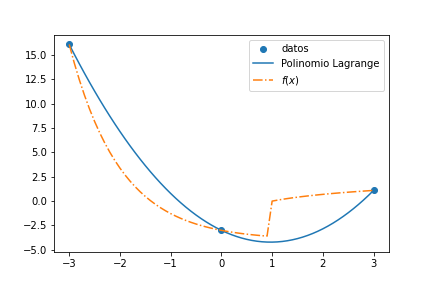
\includegraphics[width=\textwidth]{metodo-lagrange/lagrange-3-datos.png}
        \caption[Network2]%
        {{\small Polinomio de Lagrange utilizando 3 datos}}    
    \end{subfigure}
    \hfill
    \begin{subfigure}[b]{0.475\textwidth}  
        \centering 
        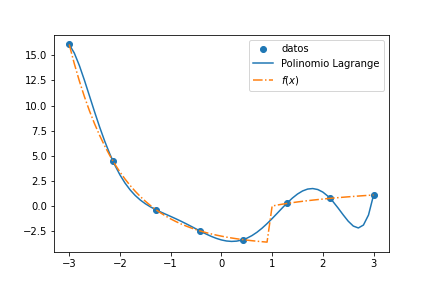
\includegraphics[width=\textwidth]{metodo-lagrange/lagrange-8-datos.png}
        \caption[]%
        {{\small Polinomio de Lagrange utilizando 8 datos}}    
    \end{subfigure}
    \vskip\baselineskip
    \begin{subfigure}[b]{0.475\textwidth}   
        \centering 
        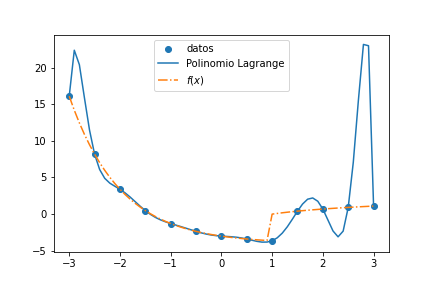
\includegraphics[width=\textwidth]{metodo-lagrange/lagrange-13-datos.png}
        \caption[]%
        {{\small Polinomio de Lagrange utilizando 13 datos}}    
    \end{subfigure}
    \hfill
    \begin{subfigure}[b]{0.475\textwidth}   
        \centering 
        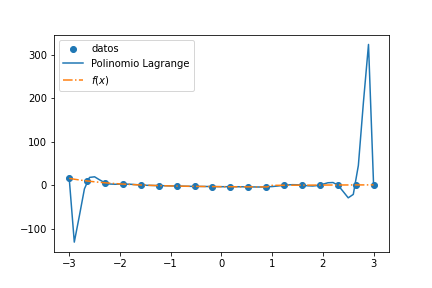
\includegraphics[width=\textwidth]{metodo-lagrange/lagrange-18-datos.png}
        \caption[]%
        {{\small Polinomio de Lagrange utilizando 18 datos}}    
    \end{subfigure}
    \caption{Ejemplo de aproximación de la función $f(x)$ a partir de los polinomios de Lagrange.} 
    \label{fig:aproximacion-lagrage}
\end{figure}

El problema que evidencia este caso patológico es el tratar de abarcar todo el dominio 
con un mismo polinomio ¿y si en lugar de eso se hicieran aproximaciones 
en una partición concreta del dominio? El resultado sería una función definida a trozos.   
La cuestión es que esta aproximación sería difícil de implementar de manera eficiente;
sin embargo, es el germen y el enfoque de las \textit{funciones de activación}. 

De todas formas no abandonemos del todo esta teoría, porque como ya veremos el 
teorema de Stone Weierstrass  \ref{ch:TeoremaStoneWeiertrass} jugará 
un papel fundamental es la demostración 
de que las redes neuronales son aproximadores universales.

\subsection*{Las funciones de activación $\Gamma$ son la clave del aprendizaje}  

Las \textit{funciones de activación} serán definidas con profundidad en la sección 
\ref{def:funcion_activacion_articulo}, pero para continuar con nuestro razonamiento 
pensemos en ellas como una función cualquiera que no sea un polinomio. 

Una vez liberados de tratar de buscar un polinomio que aproxime la función en todo
el dominio, podemos pensar en aproximar la image de acorde a intervalos.  
 
\textcolor{red}{TODO : Añadir gráficos cuando esté implementada una red neuronal}

% Ejemplo de cómo se aproxima gracias  a la forma de la función de activación
\begin{figure}[h!]
    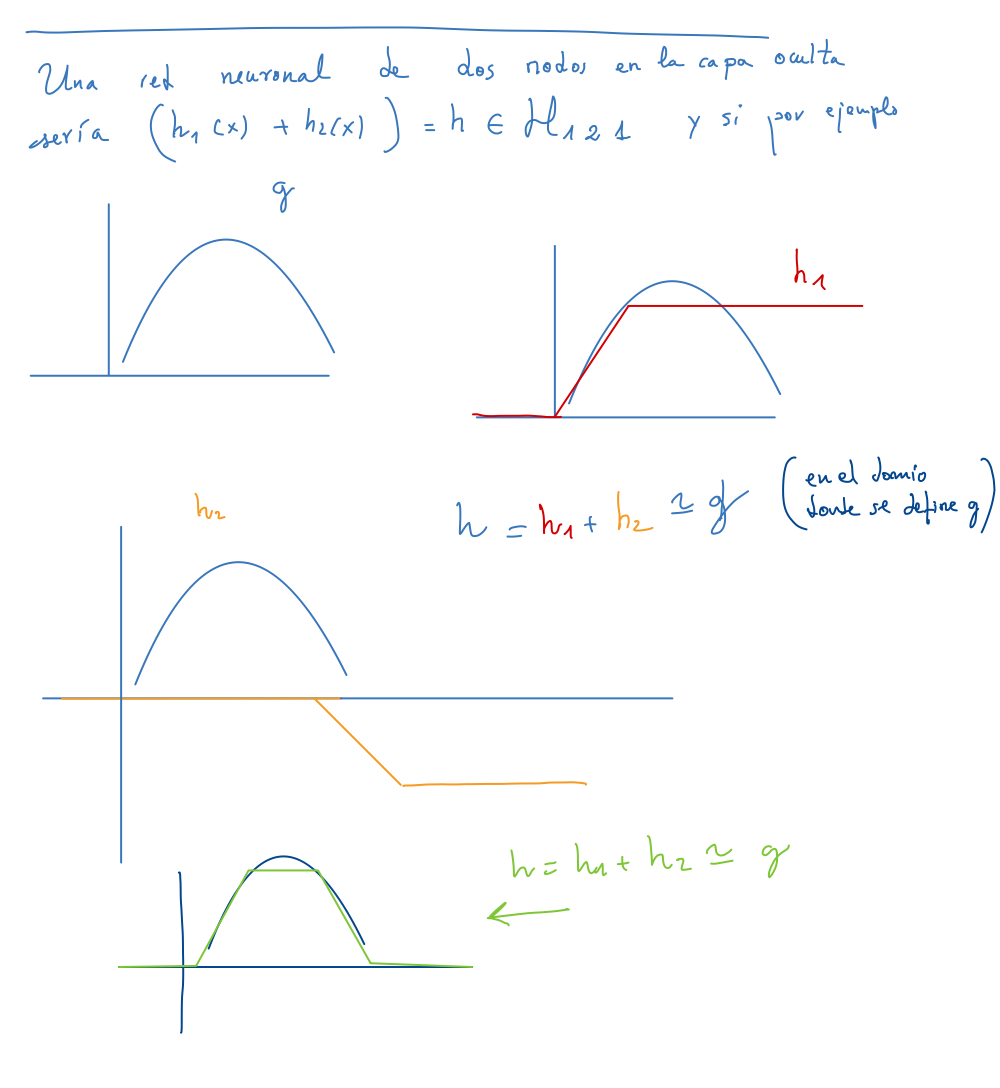
\includegraphics[width=\textwidth]{1-Introduccion_redes_neuronales/idea-como-aproxima-redes-neuronales.jpeg}
    \caption{Cómo actúa en la aproximación una función de activación}
    \label{img:idea-como-aproxima-redes-neuronales}
   \end{figure}

La idea intuitiva es que para una capa oculta con una neurona, 
lo que se hace es \textit{colocar} por escalado y simetrías la imagen de la función de activación. 

% Ejemplo trivial de como la forma de la función de activación influye en aproximar mejor 
\begin{figure}[h!]
    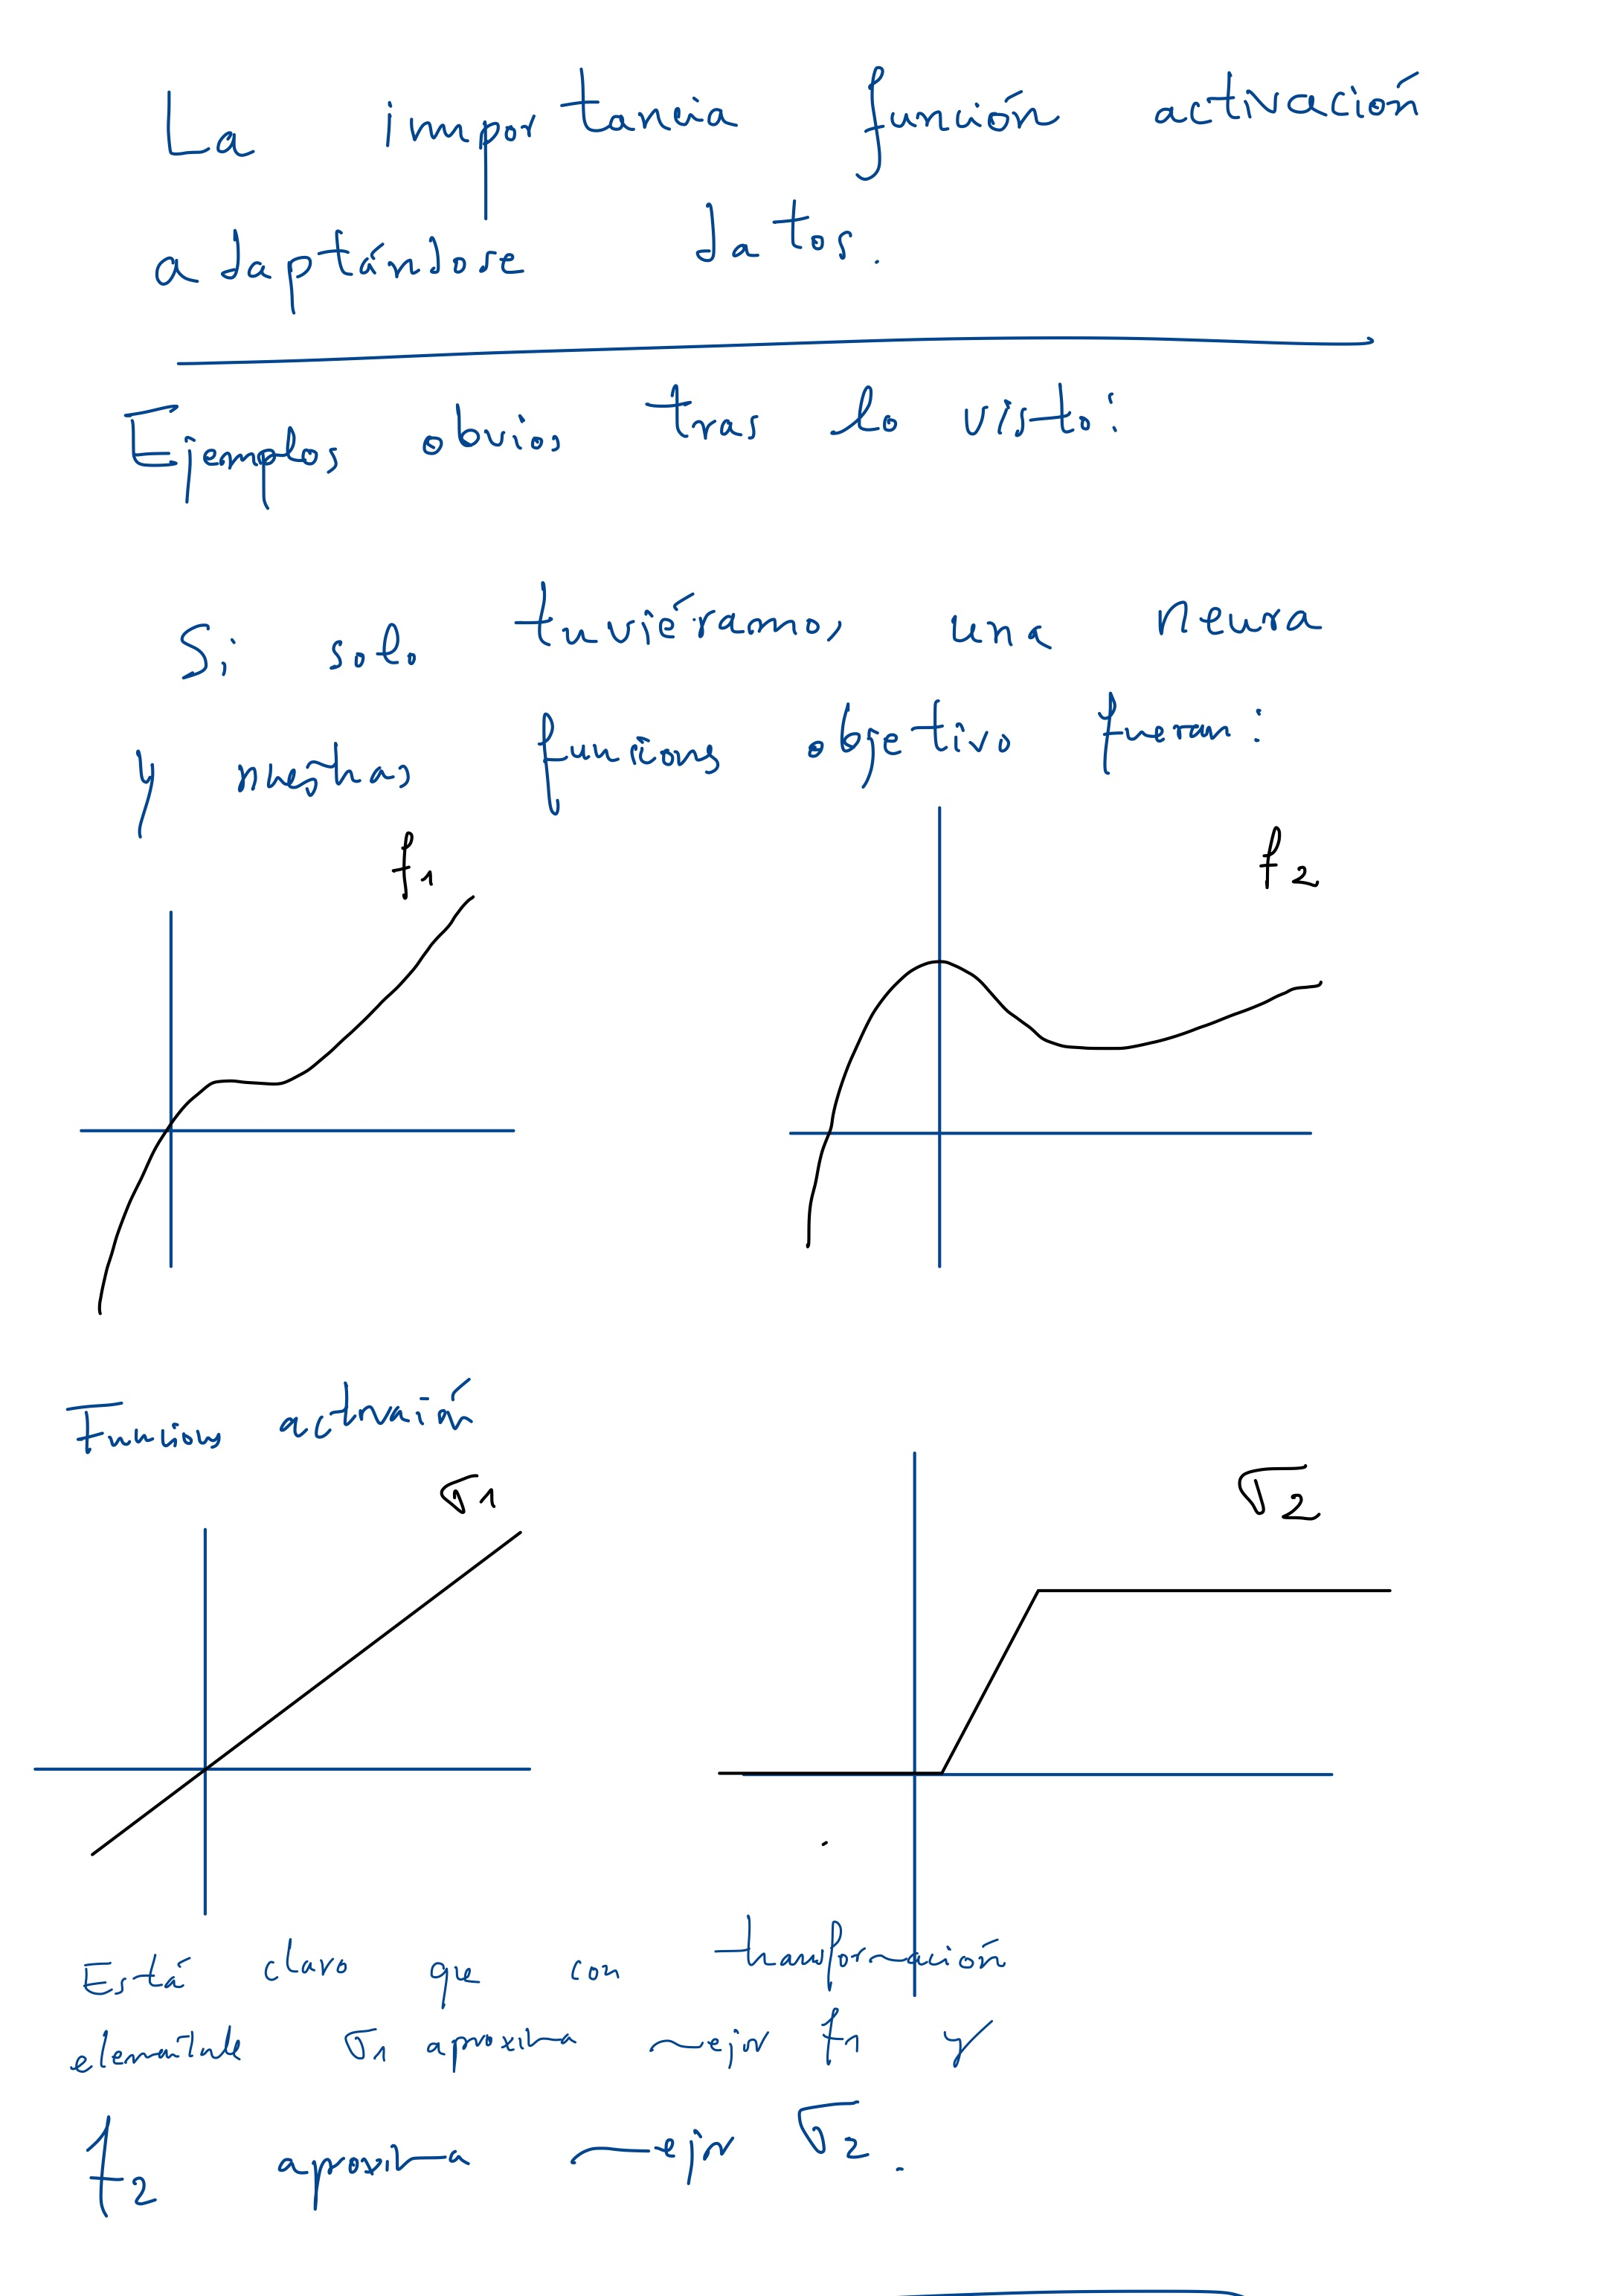
\includegraphics[width=0.8\textwidth]{1-Introduccion_redes_neuronales/Idea-forma-función-Activación.jpg}
    \caption{Cómo afecta la forma de la función de activación}
    \label{img:como afecta la forma de la función de aproximación}
\end{figure}


% Las redes neuronales multicapa son aproximadores universales 
\chapter{Las redes neuronales  son aproximadores universales}  
\label{chapter4:redes-neuronales-aproximador-universal}
% !TeX encoding = utf8
%
%*******************************************************
% Construcción redes neuronales  una capa 
%*******************************************************

\section{Definición de las redes neuronales \textit{Feedforward Networks} 
de una capa oculta} \label{sec:redes-neuronales-intro-una-capa}

% Nota margen aclarativa de una función medible
\reversemarginpar
\setlength{\marginparwidth}{\smallMarginSize}
\marginpar{\maginLetterSize
    \iconoAclaraciones \textcolor{dark_green}{     
        \textbf{Qué son las funciones medibles 
        y porqué las usamos en nuestra definición.}
    }
    {\maginLetterSize
        A nivel intuitivo una función medible es aquella,
        que por muy extraña que sea,  
        su imagen (los valores que toma su salida) está acotada casi siempre, lo que a nivel práctico 
        significa que \textit{podemos observar y cuantificar sus valores.}
    
        Con esto pretendemos que nuestra definición $\Gamma$ 
        sea lo menos restrictiva posible.
    }
}
\normalmarginpar
\setlength{\marginparwidth}{\bigMarginSize}


A lo largo de esta sección  explicaremos qué es una red neuronal, cómo está construida y en qué consiste el \textit{aprendizaje} de la misma, concretamente
construiremos el tipo particular \textit{Feedforward Neural Networks}, al cual nos referiremos de ahora
en adelante como red neuronal.

De acorde con nuestra filosofía de trabajo expuesta en la introducción del capítulo \ref{motivo-una-capa} partiremos de un modelo de una sola capa oculta. 

% Imagen grafo red neuronal  una capa oculta muy simple y en blanco y negro 
\begin{figure}[h!]
    \centering
    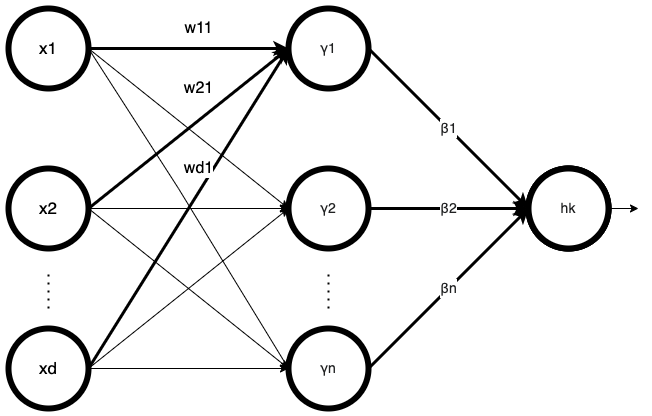
\includegraphics[width=0.85\textwidth]{1-Introduccion_redes_neuronales/Red-Neuronal-una-capa-simple.png}
    \caption{\textit{Grafo} de una red neuronal de una capa oculta}
    \label{img:grafo-red-neuronal-una-capa-oculta}
\end{figure}

\begin{definicion}[Redes neuronales de una capa oculta] \label{definition:redes_neuronales_una_capa_oculta}
    Dados $X \subseteq \R^d, Y \subseteq \R^s$ y  $\Gamma$ un conjunto no vacío de funciones medibles definidas de $\R$ a $\R$, denotaremos como 
    \begin{align}
        \mathcal{H}(X,Y) 
        =
        \{
            h : X \longrightarrow Y 
            /& \quad 
            h_k(x) = 
            \sum_{i=1}^{n} \beta_{i k} \gamma_{i}( A_{i}(x)), \\
            & \text{donde  $h_k$  es la proyección k-ésima de $h$ con 
            $k \in \{1, \ldots, s\}$}, \\
            & n \in \N,\gamma_{i} \in \Gamma , \beta_{i k} \in \R
             \text{ y }A_{i} \text{ una aplicación afín de $\R^d$ a $\R$}           
        \}.
    \end{align}
\end{definicion}
% Nota margen aclarativa de la fórmula
\marginpar{\maginLetterSize
    \iconoAclaraciones \textcolor{dark_green}{     
        \textbf{Interpretación fórmula}
    }
    {\maginLetterSize
        Observemos que $n$ es el número de neuronas de la capa oculta. Es decir lo que en el grafo \ref{img:grafo-red-neuronal-una-capa-oculta} serían las neuronas de las capas ocultas se correspondería con términos $\gamma_{i}( A_{i}(x))$.
    }
}
\normalmarginpar
\setlength{\marginparwidth}{\bigMarginSize}


Es habitual representar una red neuronal de forma matricial, veremos que tal forma es equivalente a la definición dada. 

Consideramos la aplicación inclusión 
$i: \R^r \longrightarrow \R^{r+1}$ dada por 
 $i((x_1, \ldots, x_d)) = (1,x_1, \ldots, x_d).$
Para coeficientes $w_i \in \R$ toda función afín es de la forma 
$A_{i}(x)= \sum_{j=1}^d( w_{j i} x_j) + w_{0i}$, 
tomando $W_i = (w_{0 i}, w_{1 i}, \ldots, w_{r i}) \in \R^{r+1}$ tenemos que 
$A_i(x) = W_i \cdot i(x)$ como queríamos probar. 

Además también se suele mostrar de manera pedagógica con un grafo como el mostrado en la 
figura \ref{img:grafo-red-neuronal-una-capa-oculta}.

% Elimino TODO porque ya se ha comentado.

\subsection*{Componentes de la red neuronal}  

A la vista de la definición dada notemos que cada elemento de 
$\mathcal{H}(X,Y)$ viene determinado por los coeficientes 
de las distintas $\beta$ y  $w$s de la función afín. Como veremos más adelante estos son los valores que \textit{aprende una red neuronal}.

\subsection*{Diferencia con otras definiciones}  \label{subsection:diferencia-otras-definiciones-RRNN}

En otros textos como en el capítulo cinco, páginas 227-256 del libro \cite{BishopPaterRecognition} y las notas online sobre redes neuronales de \cite{MostafaLearningFromData} se presentan las redes neuronales de una capa como 
\begin{align}
    y_k(x,w) &= \theta_k 
    \left( 
        \sum^M_{j=1} w_{ji}^{(2)}
        \sigma_j 
        \left(
            \sum_{i=1}^D w_{ji}^{(1)} x_i + w_{j0}^{(1)}
        \right)
        + w_{k0}^{(2)}
    \right) 
    \\
    & = 
    \theta_k 
    \left( 
        \sum^M_{j=1} A^{(n_k)}_{k}
        \left(
            \sigma 
            \left(
                A^{r}_{j k}
                \left(
                    x
                \right)
            \right)
        \right)
    \right)
    \text{ para cada  } k \in \{1, \ldots, K \}.
\end{align}

Donde $\theta_k$ representa una función de \textit{clasificación}, 
$\sigma_j$ lo que se suele llamar \textit{función de activación} y a la que además se le exige que sea diferenciable.

Las diferencias con nuestra definición son las siguientes 
\begin{itemize}
    \item \textbf{Desaparece la función de clasificación $\theta$}. El motivo es que es un artificio teóricamente innecesario de acorde al teorema de convergencia universal \ref{teo:MFNAUA}.
    \item \textbf{Se elimina un parámetro} de la transformación afín de la última capa, puesto que no es necesario para la convergencia de nuevo por \ref{teo:MFNAUA} lo hemos eliminado.
    \item Nuestras funciones de activación son funciones medibles en vez de diferenciables ya que a priori no existe ninguna hipótesis teórica que fuerce a tal restricción.
\end{itemize}

\subsection*{Las funciones de activación $\Gamma$ son la clave del aprendizaje}  

Notemos que de no ser por las funciones de activación se estarían haciendo transformaciones lineales de los datos, por el contrario estamos realizando \textit{cambios más fuerte} siendo capaz con esto de \textit{de diferenciar puntos claves}.

\textcolor{red}{Dicho de esta manera queda muy poco claro y habría que profundizar más.}
Vamos a mostrar un ejemplo de la importancia de la función de activación 

\textcolor{red}{TODO : Añadir gráficos cuando esté implementada una red neuronal}


% Ejemplo de cómo se aproxima gracias  a la forma de la función de activación
\begin{figure}[h!]
    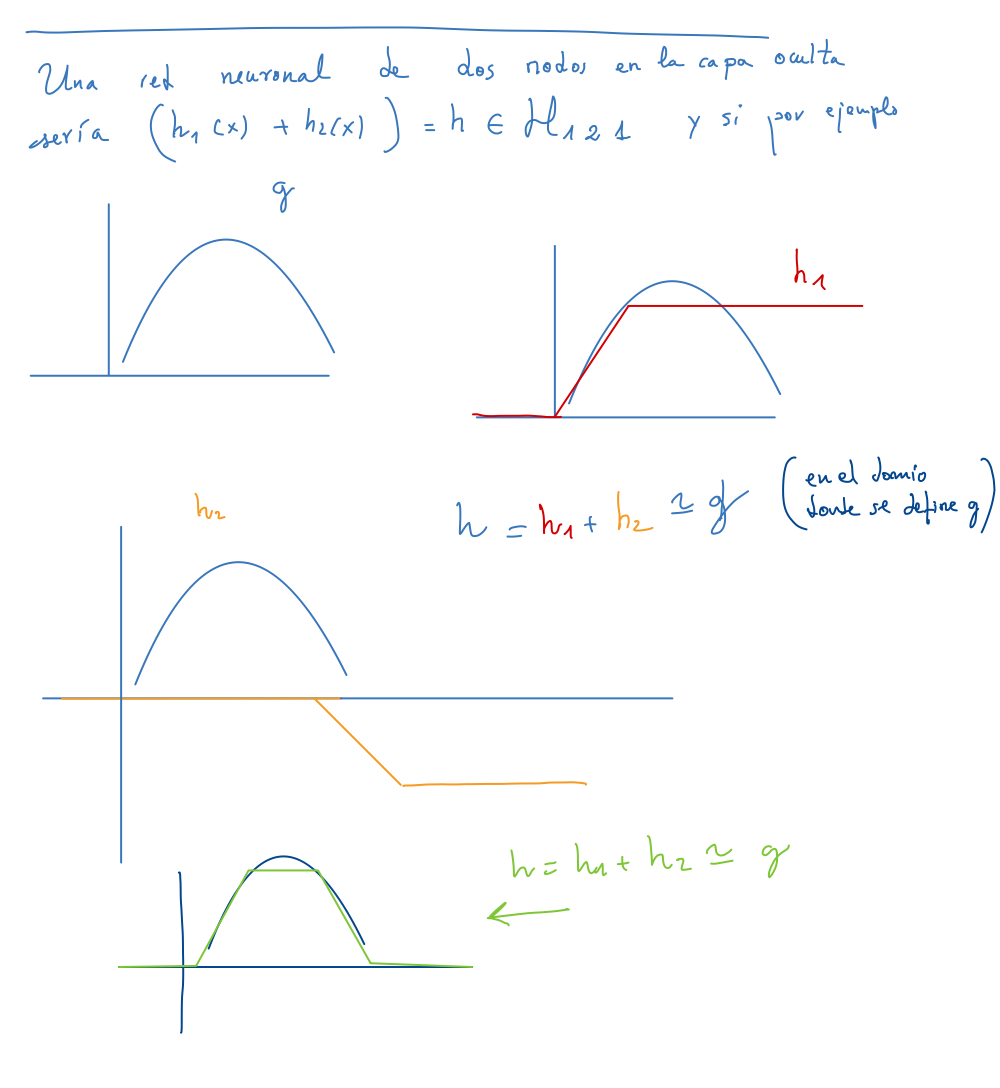
\includegraphics[width=\textwidth]{1-Introduccion_redes_neuronales/idea-como-aproxima-redes-neuronales.jpeg}
    \caption{Cómo actúa en la aproximación una función de activación}
    \label{img:idea-como-aproxima-redes-neuronales}
   \end{figure}

La idea intuitiva es que para una capa oculta con una neurona, 
lo que se hace es \textit{colocar} por escalado y simetrías la imagen de la función de activación. 

% Ejemplo trivial de como la forma de la función de activación influye en aproximar mejor 
\begin{figure}[h!]
    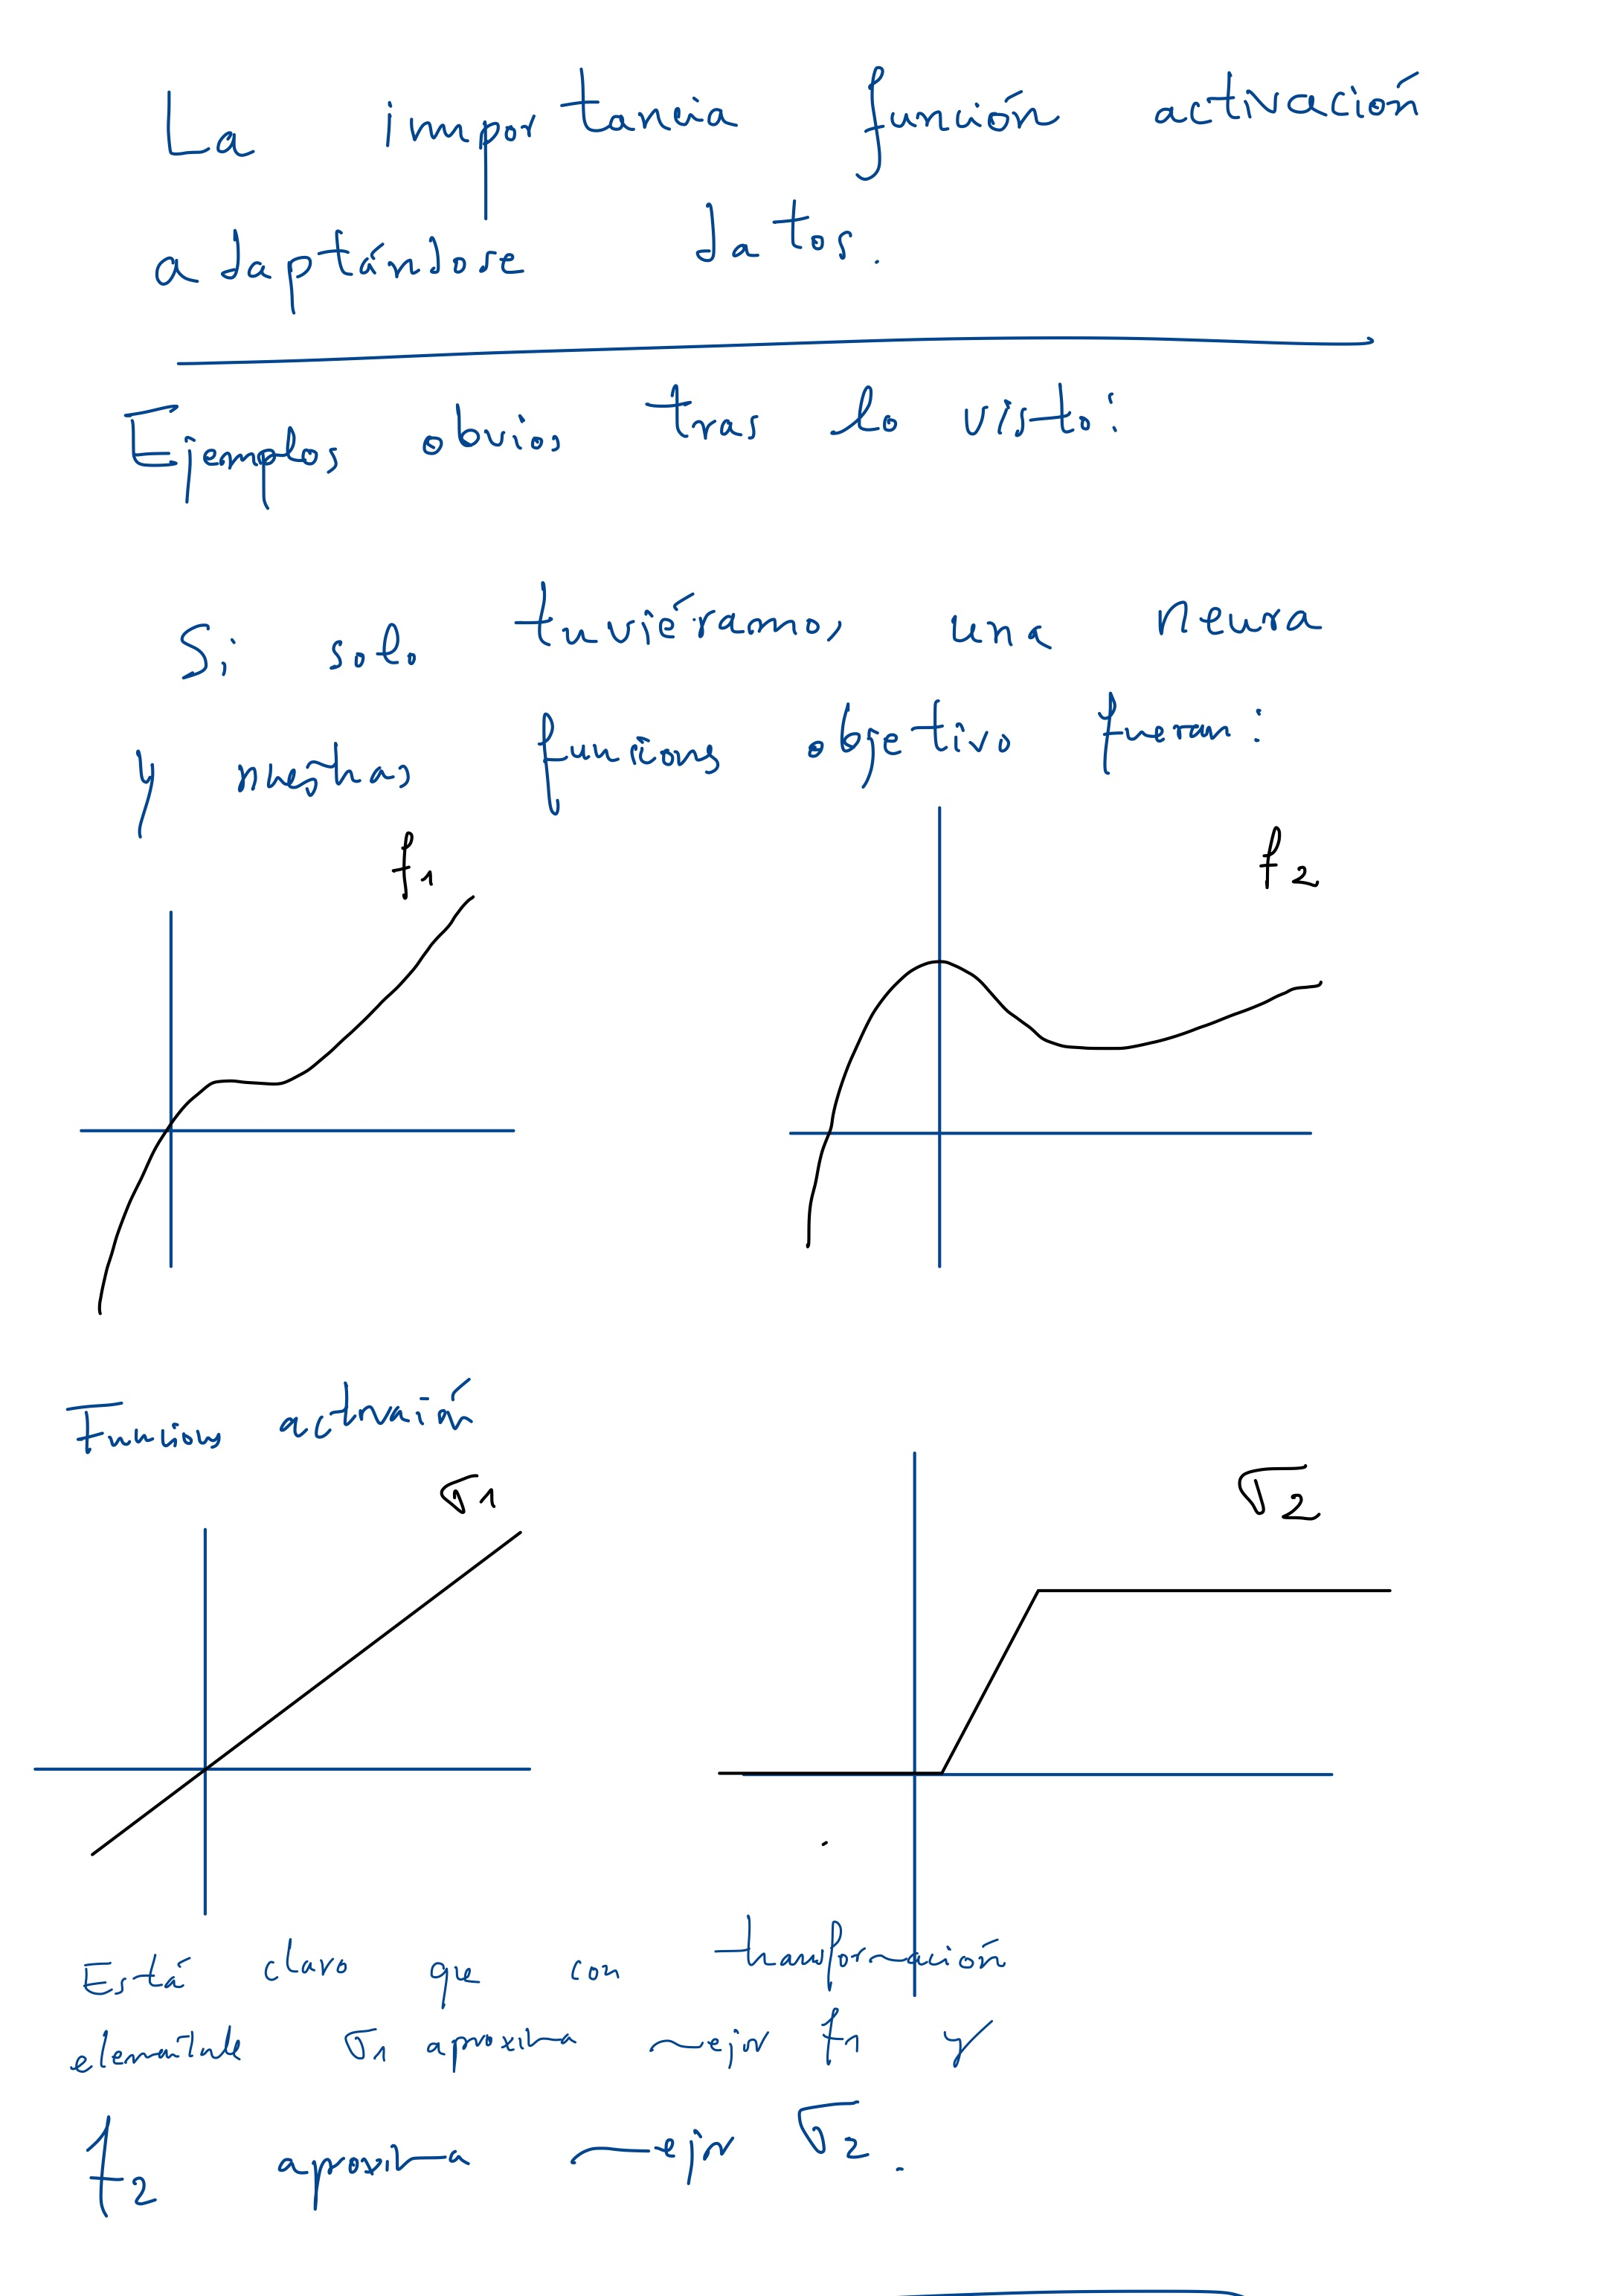
\includegraphics[width=0.8\textwidth]{1-Introduccion_redes_neuronales/Idea-forma-función-Activación.jpg}
    \caption{Cómo afecta la forma de la función de activación}
    \label{img:como afecta la forma de la función de aproximación}
   \end{figure}

% IDEA
\iconoAclaraciones \textcolor{dark_green}{ Nota idea Blanca: Multiplicar por un coeficiente complejo sería aplicar un giro,
 lo que a priori mejoraría la convergencia
 ¿Qué pasaría se cambiáramos el cuerpo?}

Ante esta idea habría que plantearse si: 

\begin{enumerate}
    \item Formalizar si esto mejoraría.
    \item A nivel de implementar Julia tiene números complejos ¿cuánto supondría de coste computacional? ¿merecería la pena?
    \item ¿Cómo habría que actualizar los pesos?
\end{enumerate}

% IDEA
\iconoAclaraciones \textcolor{dark_green}{ Nota idea Blanca: Vista esta idea sería muy interesante plantearse a partir de los datos cómo deberían de ser las funciones de activación. Es decir, que no se fijen a priori, sino que sean de los datos donde provenga su forma.}

Para poder utilizarse la idea que acaba de plantearse debería de plantearse: 
\begin{enumerate}
    \item Formalizar beneficio teórico.
    \item Balanza costo y mejora.
    \item Una forma de mejorar que acepte esas funciones (no necesariamente \textit{backpropagation}).
\end{enumerate}

% IDEA
\iconoAclaraciones \textcolor{dark_green}{ Nota idea Blanca: Ante esto mi intuición me dice que que la función de activación sea constante por algún extremo y que no fuera constante en algún intervalo serían las únicas hipótesis para que tal función de activación sirviera para construir redes neuronales que funcionara como aproximador universal}



% !TeX root = ../../tfg.tex
% !TeX encoding = utf8
%
%*******************************************************
% Introducción artículo MFNAUA
%*******************************************************
\section{Las redes neuronales son aproximadores universales}  

Tras las definición \ref{sec:redes-neuronales-intro-una-capa} de red neuronal expuesta,
es pertinente la pregunta si tal estructura será 
capaz de aproximar con éxito una función genérica desconocida.   

Aunque las redes neuronales multicapa ya se venían aplicando con anterioridad, 
véase por ejemplo los usos expuestos durante la primera conferencia
internacional de redes neuronales de \cite{4307059} de 1987, 
no fue hasta 1989 que se descubrió formalmente su alcance.
 Tal delimitación se propuso en el artículo 
\textbf{Multilayer Feedforward Networks are Universal Approximators} \cite{HORNIK1989359}
 escrito por Kurt Hornik, Maxwell Stinchcombe y Halber White enunciando: 

\begin{teorema}\textbf{Las redes \textit{feedforward} multicapa son una clase de aproximadores universales } \label{teo:MFNAUA}
    \\
    Una red neuronal \textit{feedforward} multicapa estándar con tan solo una capa oculta y con una función de activación cualquiera es capaz de aproximar cualquier 
    función Borel medible  con dominios y codominios de dimensión finita (no necesariamente iguales) y con el nivel de precisión que se desee siempre y cuando 
    se utilicen suficientes neuronas. En este sentido las redes \textit{feedforward} multicapa son una clase de aproximadores universales.

\end{teorema}

En las secciones siguientes, con el fin de alcanzar una
 comprensión profunda de las redes neuronales,
trataremos de desgranar y profundizar en el artículo y su 
demostración. Primero precisaremos o introduciremos conceptos elementales 
sobre redes neuronales \ref{ch:articulo:sec:defincionesPrimeras}, después 
demostraremos el teorema en el caso real 
\ref{teo:TeoremaConvergenciaRealEnCompactosDefinicionesEsenciales} e iremos refinando y generalizando los resultados hasta probar
el resultado enunciado \ref{teo:MFNAUA} para una capa oculta.

 % Nota margen de denso
 \setlength{\marginparwidth}{\bigMarginSize}
 \marginpar{\maginLetterSize
     \iconoAclaraciones \textcolor{dark_green}{ 
         \textbf{Idea intuitiva conjunto denso.}
     }
     Si $S$ es denso en $T$, 
     se está está diciendo que \textbf{los elementos de $S$ son capaces de aproximar cualquier elemento de $T$
     con la precisión que se desee}. 
 }

 
El esquema general será: 

\begin{align*}
    \rrnn 
        \xRightarrow[]{\ref{teo:2_4_rrnn_densas_M}}  
    \rrnng 
        \xRightarrow[]{\ref{teorema:2_3_uniformemente_denso_compactos}}
    \pmcg
        \xRightarrow[]{\ref{teo:TeoremaConvergenciaRealEnCompactosDefinicionesEsenciales}}     
    \fC    
        \xRightarrow[]{\ref{teo:2_2_denso_función_continua}} 
    \fM.
\end{align*}

   

\begin{itemize}
    \item Las redes neuronales que nosotros hemos modelizado son densas en un espacio más general que hemos denominado \textit{Anillo de aproximación de redes neuronales}
    generado a partir de una función de activación $\psi$. 
    \item Que a su vez es denso en el \textit{Anillo de aproximación de redes neuronales}
    generado a partir de una función medible $G$. 
    \item El espacio \textit{Anillo de aproximación de redes neuronales} es denso en el de las funciones continuas.
    \item Las funciones continuas son densas en el espacio de funciones medibles. 
\end{itemize}

Si quisiéramos situar en este esquema a otras definiciones de redes neuronales las situaríamos entre  nuestro modelo y el espacio \textit{Anillo de aproximación de redes neuronales}; en  el capítulo \ref{chapter:construir-redes-neuronales} se probará tal resultado y analizarán los beneficios de basarnos en un modelo más simple. 



% !TeX root = ../../tfg.tex
% !TeX encoding = utf8
%
%*******************************************************
% Contenido del artículo 1: Definiciones primeras
%*******************************************************

\section{Definiciones primeras}\label{ch:articulo:sec:defincionesPrimeras}  

Comenzaremos presentando definiciones básicas sobre redes neuronales. 


\begin{definicion}[Función de activación] \label{def:funcion_activacion_articulo}
    Una función  $\psi: \R \longrightarrow [0,1]$ es una \textbf{ función de activación} si  cumple las siguientes propiedades:
    \begin{enumerate}[label=(\roman*)]
        \item Es no decreciente.
        \item $\lim _{x \rightarrow \infty} \psi(x) = 1
        $.
        \item $\lim _{x \rightarrow -\infty} \psi(x) = 0$.
    \end{enumerate}  
   
    Ejemplos comunes de funciones de activación son

    %%% Nota sobre funciones activación más democráticas que otras
    \marginpar{\maginLetterSize
         \iconoProfundizar \textcolor{blue}{    
        \textbf{Observación sobre la idoneidad de cada función activación:}
    }
    Se probará la convergencia de las redes neuronales independientemente de la función de activación seleccionada. Cabe entonces la pregunta
    ¿Existen funciones de activación más democráticas que otras? 
    Se discutirá esta pregunta en \ref{funciones-activacion-democraticas-mas-demoscraticas}.
    }

    % Imágenes de la función indicadora 
    \begin{figure}[h]
        \centering
        \begin{subfigure}[t]{0.47\textwidth}
            \centering
            \includegraphics[width=\textwidth]{
                articulo_rrnn_aproximadores_universales/función_indicadora_l_0.png}
            \caption{Función indicadora $\lambda_0 = 0$}  
            \label{fig:función_indicadora}
        \end{subfigure}
        \hfill
        \begin{subfigure}[t]{0.47\textwidth}  
            \centering 
            \includegraphics[width=\textwidth]{articulo_rrnn_aproximadores_universales/función_umbral_lineal.png
            }
            \caption{Función umbral $w=(2)$, $t=1$}    
            \label{fig:función_umbral_lineal}
        \end{subfigure}
        \begin{subfigure}[t]{0.47\textwidth}   
            \centering 
            \includegraphics[width=\textwidth]{articulo_rrnn_aproximadores_universales/función_rampa.png}
            \caption{Función rampa} 
            \label{fig:funciones_rampa}
        \end{subfigure}
        \hfill
        \begin{subfigure}[t]{0.47\textwidth}   
            \centering 
            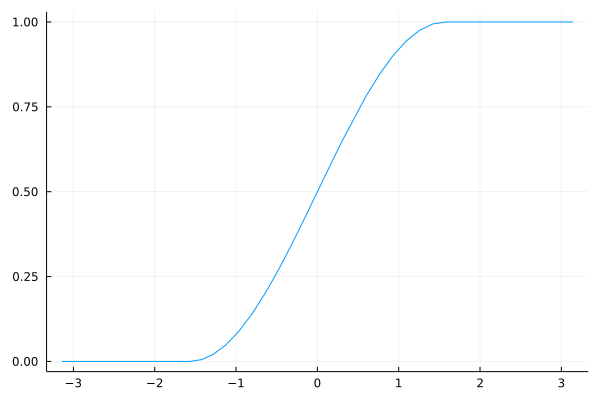
\includegraphics[width=\textwidth]{articulo_rrnn_aproximadores_universales/cosineSquasherSinTitulo.png}
            \caption{\textit{Cosine Squasher}}   
            \label{fig:cosine_squasher}
        \end{subfigure}
        \caption{Ejemplos de funciones de activación} 
        \label{fig:EjemplosFunciónActivación}
    \end{figure}

    \begin{itemize}
        \item \textbf{Funciones indicadoras} \ref{fig:función_indicadora}: $\psi(\lambda) = 1_{\{\lambda > \lambda_0\}}$ con $\lambda_0 \in \R$. 
        
        \item \textbf{Funciones umbral} \ref{fig:función_umbral_lineal}:
        Una función umbral, es una función booleana monótona $\psi_w: \{0,1\}^n \longrightarrow \{0,1\},$ 
        donde para $w \in \R^n$, $t \in \R$ fijos se
        satisface que 
        \begin{equation}
            \psi_w(x) = \left\{
                \begin{array}{lcc}
                    1, &   si  & w \cdot x \geq t \\
                    0, &  si & w \cdot x < t.\\
                    \end{array}
            \right.
        \end{equation}
        
        \item \textbf{Función rampa} \ref{fig:funciones_rampa}: $\psi(\lambda)  = \lambda 1_{\{0 \leq \lambda \leq  1\}} + 1_{\{\lambda > 1\}}.$
    
        \item \textbf{La función \textit{cosine squasher}} de Gallant and White 
        \ref{fig:cosine_squasher} (1988) \cite{Gallant88thereexists}. 
        \begin{equation*}
    \psi(\lambda )= \left(1 + \cos\left(\lambda + 3 \frac{\pi}{2} \right) \frac{1}{2}\right) 
     1_{\{\frac{-\pi}{2} \leq \lambda \leq  \frac{\pi}{2}\}}
     +
     1_{\{ \frac{\pi}{2} < \lambda \}}.
    \end{equation*}
    \end{itemize}

   Notemos que así definidas las funciones de activación son medibles, ya que la imagen inversa de un abierto de $[0,1]$ siempre será un conjunto medible de  $\R$  (capítulo 7  página 77 \cite{nla.cat-vn1819421}).
    

    Cabe destacar que la definición tomada es la propuesta en \cite{HORNIK1989359} y que existen
    otras posibles definiciones menos restrictivas con las que también se ha probado la convergencia universal.
    Por ejemplo podrían aceptarse funciones de activación no continuas (véase \cite{FUNAHASHI1989183}); 
    o como 
    se demuestra en \cite{DBLP:journals/corr/SonodaM15} y en \cite{non-polynomial-activation-functions}, funciones de activación no polinómicas y no acotadas. 
\end{definicion}

% Nota sobre que la funciones de activación 
% son clave en el aprendizaje
\setlength{\marginparwidth}{\smallMarginSize}
\marginpar{\maginLetterSize
    \iconoClave  \textcolor{darkRed}{     
        \textbf{
            Las funciones de activación $\Gamma$ son la clave del aprendizaje
        }
    }
    \label{ch03:funcionamiento-intuitivo-funcion-activacion}

La idea intuitiva es que cada neurona 
lo que se hace es \textit{colocar} por transformaciones afines la imagen de la función de activación en el espacio con el fin 
de aproximar una región de la imagen de la función ideal. 
Por lo tanto, la forma que ésta tenga será determinante en el número de neuronas necesarias para la convergencia.    
}
\setlength{\marginparwidth}{\bigMarginSize}

% Fin del tratamiento de funciones de activación 

Para cualquier natural $d$ mayor que cero  denotaremos por $\afines$ al conjunto de todas 
las \textbf{funciones afines} de $\R^d$ a $\R$. Es decir el conjunto de funciones de la forma 
$A(x) = w \cdot x + b$ donde $x$ y $w$ son vectores de $\R^d$,  $b \in \R$ es un escalar
 y $\cdot$ representa el producto escalar
usual. En este contexto, $x$ corresponde al vector entrada de la red neuronal, $w$ los pesos de la red
que se multiplicarán con $x$ en la capa intermedia y $b$ el sesgo. 

   % Nota margen sobre que abstrae esta estructura de red neuronal
 \marginpar{\maginLetterSize
 \iconoAclaraciones \textcolor{dark_green}{     
 \textbf{Idea tras la definición de $\pmc$.}
 }
Nótese que de acorde a la definición  \ref{definition:redes_neuronales_una_capa_oculta}
lo que se está refiriendo es la clase de las redes 
neuronales de una capa oculta y \textbf{salida de una dimensión}.
Donde cada sumando representa una neurona de la capa oculta.
}
%%% fin nota
\begin{definicion} [Formalización de una red neuronal de una capa oculta y salida real]
    Para cualquier función Borel medible $G$, definida de $\R$ a $\R$ y cualquier natural positivo
    $d \in \N$ se define a la clase de funciones $\pmc$ como 

    \begin{equation}
        \begin{split}
        \pmc = 
        \{ 
            & f: \R ^d \longrightarrow \R / \quad
            f(x)=\sum_{j = 1} ^q (
            \beta_j G(A_{j}(x))), \\
            & x  \in \R ^d, \beta_j \in \R, A_{j}\in \afines,q \in \N
        \}.
        \end{split}
    \end{equation}

    Conforme avancen los resultados teóricos veremos que $\pmc$ 
    no depende de la función $G$ seleccionada; así pues, tras enunciar tales resultados nos referiremos sin ambigüedad a tal conjunto como $\rrnn$.
\end{definicion}


Definiremos a continuación una familia de funciones más generales que $\pmc$ con la intención de que actúe como nexo de unión entre la clase de funciones continuas y las redes neuronales de una capa facilitándonos con ello la prueba de los resultados. La familia que introduciremos solo tiene 
una utilidad teórica, es decir no tendrá ninguna relevancia a nivel práctico en cuanto a implementaciones.
   
% Nota margen sobre Idea intuitiva de la definición 
\marginpar{\maginLetterSize
\iconoAclaraciones \textcolor{dark_green}{     
\textbf{Motivación de la definición de $\pmcg$}}.

En un principio será más fácil demostrar que con 
funciones de esta clase seremos capaz de aproximar cualquier función continua.
De esta manera este conjunto actuará de nexo de unión entre las funciones continuas y las redes neuronales 
facilitando las demostraciones. De ahora en adelante nos
 referiremos a este conjunto como al \textbf{de anillo de aproximación} (como curiosidad, el nombre proviene a que
  tiene estructura de anillo y que se utilizará para 
  aproximar funciones continuas).
}
\begin{definicion} [Anillo de aproximación de redes neuronales]\label{def:articulo_abstracción_rrnn}
    
    \begin{equation} 
        \begin{split}
        \sum \prod^d(G) = \{ 
        &f: \R^r \longrightarrow \R / \quad
        f(x) = \sum_{j = 1} ^q  \beta_j \prod_{k=1}^{l_j}
        G(A_{jk}(x)), \\
        &x  \in \R^d, \beta_j \in \R, A_{jk}\in \afines; l_j,q \in \N
        \}.
    \end{split}
    \end{equation}  

 
    Notemos que $\pmc$ se recupera en el caso particular en el que $l_j = 1$ para todo $j$.
    Los elementos de $\pmcg$ son combinaciones lineales de productos finitos de neuronas. 

\end{definicion}

\reversemarginpar
  %%% Nota margen sobre función medible 
  \setlength{\marginparwidth}{\smallMarginSize}
  \marginpar{\maginLetterSize
    \iconoAclaraciones \textcolor{dark_green}{     
        \textbf{
            Aplicación práctica aprendizaje automático y 
            relación con las funciones medible.
        }
    }
    \textbf{A nivel práctico se tiene un conjunto de datos
    para los cuales queremos extraer un patrón} que nos permita 
    predecir la naturaleza de datos nuevos. Es por ello necesario
    suponer que estos datos están regidos por alguna regla, la cual 
    puede ser todo lo extraña posible pero que toma valores 
    que pueden ser observables y cuantificables en la mayoría de los casos, estos comportamientos son formalizados
     matemáticamente con \textbf{funciones medibles}.
}
\setlength{\marginparwidth}{\bigMarginSize}
\normalmarginpar 

Introducimos a continuación la notación de los conjuntos de funciones que seremos capaces de aproximar.  

Denotamos por  $\fC$ al conjunto de funciones continuas con dominio en $\R^d$ y codominio $\R$,
por  $\fM$ al conjunto de todas las funciones Borel medibles de $\R^d$ a $\R$; 
y por $B^d$ a la $\sigma$-álgebra de Borel en $\R ^d$. 

En lo que respecta a definiciones anteriores, $\pmc$ y $\pmcg$ están contenidos en
$\fM$ para cualquier función Borel-medible $G$. Si $G$ es continua entonces 
$\pmc$ y $\pmcg$ pertenecen a $\fC$. Tengamos presente que $\fC$ es un subconjunto
de $\fM$.  

De ahora en adelante nos referiremos a Borel-medible como medible. 
  

\subsection{ Reflexión sobre el tipo de funciones que se pueden aproximar}

La existencia de funciones no medibles manifiesta una limitación
de la formalización actual de las redes neuronales que plantea las siguientes 
preguntas: 
\begin{enumerate}
    \item ¿Supone la existencia de este tipo de funciones una verdadera limitación a nivel práctico?
    \item ¿Se podría construir alguna arquitectura que sí que las aproximara?
\end{enumerate}  

Continuando con el hilo de la segunda cuestión, si se carece de un espacio vectorial, 
de una medida,  ¿Cómo se podría construir una sucesión de funciones que se aproxime?
Quizás habría que buscar características más intrínsecas del problema en cuestión, 
razonamientos topológicos.

\begin{definicion} [Subconjunto denso]
    % Nota margen de denso
    \reversemarginpar 
    \marginpar{\maginLetterSize
        \iconoAclaraciones \textcolor{dark_green}{ 
            \textbf{Idea intuitiva conjunto denso.}
        }
        Si $S$ es denso en $T$, 
        se está está diciendo que \textbf{los elementos de $S$ son capaces de aproximar cualquier elemento de $T$
        con la precisión que se desee}. 
    }
    \normalmarginpar

    Dado un subconjunto $S$ de un espacio métrico $(X, \rho)$, se dice que $S$ es denso por la distancia $\rho$
    en subconjunto $T$ si para todo $\varepsilon$ positivo y cualquier $t \in T$ existe un $s \in S$ tal 
    que $\rho(s,t) \leq \varepsilon$. 
\end{definicion}

Un ejemplo habitual es en el espacio métrico $(\R, |\cdot|)$ con $|\cdot|$ el valor absoluto, el subconjunto 
$T = \R$ y $S$ los números irracionales, $S = \R \setminus \Q$. 


\begin{definicion} 
    Un subconjunto $S$ de $\fC$ se dice que es \textbf{uniformemente denso para compactos} en  $\fC$
    si para cada subconjunto compacto $K \subset \R^d$ se tiene que $S_K$ es denso según $\rho_K$ en $\fC$
    donde $\rho_K$ está definida como sigue.
    Para cualquier $f,g \in \fC$ 
    \begin{equation}
        \rho _ K (f,g) = \sup_{x \in K} |f(x) - g(x)|.
    \end{equation}

    % Nota intuitiva de compacto
    \marginpar{\maginLetterSize
        \iconoAclaraciones \textcolor{dark_green}{ 
          \textbf{Noción intuitiva de compacto}
        }

        Un compacto es un conjunto que \textbf{se puede cambiar por un subconjunto finito cometiendo un error prefijado}. 

        Al trabajar con números reales, un espacio es compacto si es cerrado y acotado, lo que a nivel práctico significa que los
        \textbf{datos de entrada se encuentran dentro de un rango concreto}. 
      }

      % Nota intuitiva de uniformemente denso
      \marginpar{\maginLetterSize
        \iconoAclaraciones \textcolor{dark_green}{ 
          \textbf{Noción intuitiva de uniformemente denso para compactos }
        }
          lo que indica es que \textit{controlamos} \textbf{cuánto de cerca
          están dos funciones sea cual sea cualquier punto del compacto en que evaluemos} es decir, podríamos afirmar que para una red neuronal que tome valores por ejemplo en $[0,1]^r$, se puede saber que su error es menor que $\varepsilon \in\R^+$ independientemente de la entrada.
      }
      
\end{definicion}

\begin{definicion}
    Una serie de funciones $\{f_n\}$ \textbf{converge uniformemente a una función $f$ sobre compactos} si para 
    cada  conjunto compacto $K \subset \R^d$  se cumple que
    \begin{equation}
        \rho_k (f_n, f) \longrightarrow 0 \text{ cuando } n \longrightarrow \infty.
    \end{equation} 
\end{definicion}


% !TeX root = ../../tfg.tex
% !TeX encoding = utf8
%
%*******************************************************
% Contenido del artículo 2: Primeros resultados
%*******************************************************


\section{Primeros resultados} 
% Introducción sección 


%%%%% primer teorema de convergencia  
% Teorema 2.1 
\begin{teorema} [Teorema de convergencia real en compactos]  \label{teo:TeoremaConvergenciaRealEnCompactosDefinicionesEsenciales}

    Sea G cualquier función continua no constante definida de $\R$ en $\R$. 
    Se tiene que $\pmcg$ es uniformemente denso para compactos en $\fC$.
\end{teorema}

\begin{proof}
    Bastará probar que el conjunto $\pmcg$ satisface las hipótesis del teorema de
     Stone-Weierstrass \ref{ch:TeoremaStoneWeiertrass}.
    Lo primero será comprobar que $\pmcg$ es un álgebra, para ello veamos que:         
    \begin{enumerate}
        \item La función constante uno pertenece al conjunto. 
        Como $G$ no es constante existirá un valor de la imagen distinto de $0$, supongamos que $G(a)= b \neq 0$ para $a,b \in \R.$
        Consideremos la función afín $A(x) = 0 \cdot x + a$, está claro que $\frac{1}{b}G(A(x))$ es la función constantemente uno. 
        \item El conjunto $\pmcg$ es cerrado para sumas y producto por escalares reales. 
        En efecto, si $f,g$ pertenecen a  $\pmcg$, serán de la forma
         $f = \sum_{j = 1} ^q  \beta_{fj} \prod_{k=1}^{l_{fj}}  G(A_{fjk}(x))$ y 
        $g = \sum_{j = 1} ^p  \beta_{gj} \prod_{k=1}^{l_{gj}}G(A_{gjk}(x))$  por lo que
        \begin{equation}
            \begin{split}
                \gamma f+ \sigma g =& \gamma \sum_{j = 1} ^q  \beta_{fj} \prod_{k=1}^{l_{fj}}  G(A_{fjk}(x)) + 
                \sigma \sum_{j = 1} ^p  \beta_{gj} \ \prod_{k=1}^{l_{gj}}G(A_{gjk}(x)) \\
                & = \sum_{j = 1} ^q  (\gamma \beta_{fj})  \prod_{k=1}^{l_{fj}}  G(A_{fjk}(x)) + 
                \sum_{j = 1} ^p  (\sigma \beta_{gj}) \ \prod_{k=1}^{l_{gj}}G(A_{gjk}(x)).
            \end{split}
        \end{equation}
        
        Basta renumerar una de las sumatorias para ver $\gamma f+ \sigma g$ como una combinación 
        lineal de productos finitos de perceptrones y por tanto $\gamma f+ \sigma g \in \pmcg.$
        
        \item Cerrado para producto. Para $f,g \in \pmcg$, se tiene que $fg$ pertenece a $\pmcg$. 
        Renombrando los índices de la sumatoria con $\Lambda = i\{1..l_i\} \cup j\{1..l_j\}$ basta ver que 
        \begin{equation}
            \begin{split}
                fg &= \left(\sum_{i \in I_f} \beta_{j}  \prod_{k=1}^{l_{i}}  G(A_{ik}(x))\right)
                    \left(\sum_{j \in I_g}   \beta_{j}  \prod_{k=1}^{l_{j}} G(A_{jk}(x)) \right) \\
                    & = \sum_{i \in I_f} \left(  \beta_{j}  \prod_{k=1}^{l_{i}}  G(A_{ik}(x))
                        \left( \sum_{j \in I_g}  \beta_{j} \prod_{k=1}^{l_{j}} G(A_{jk}(x))  \right)  
                     \right) \\
                    & =  \sum_{(i,j) \in I_f \times I_g} (\beta{i}\beta{j}) \prod_{k \in \Lambda} G(A_{k}(x))
            \end{split}
        \end{equation}
        luego $fg \in \pmcg$. 
    \end{enumerate}

    Veamos que $\pmcg$ separa puntos cada compacto $K \subset \R^r$. 

    Por ser $G$ no constante existirán $a,b \in \R$ distintos cumpliendo que $G(a) \neq G(b)$. Fijadas $x,y \in K$ tomamos entonces cualquiera de las 
    funciones afines que cumplen que $A(x) = a$ y $A(y)=b$ 
    \footnote{Sabemos que al menos una habrá, ya que podemos plantear la función afín
    como un sistema de ecuaciones lineales de $r+1$ incógnita y 2 soluciones}, 
    por lo que $G(A(x)) \neq G(A(y))$ y tenemos como buscábamos que $\pmcg$ separa los puntos de $K$. 

    Veamos finalmente que para todo punto de $K$ existe una función de $\pmcg$  en el que la imagen no es nula.  

    Por ser $G$ no constante volvemos a tomar un $a \in \R$ tal que $G(a) \neq 0$ , consideramos ahora la aplicación lineal
    $A(x) = 0 \cdot x + a$ por lo que para todo $x \in K$, $G(A(x)) = G(a) \neq 0$. 

    Como hemos comprobado se verifican todas las hipótesis del teorema de Stone-Weierstrass, con lo que concluimos, como queríamos probar que $\pmcg |_K$ es denso en $C(K). $ 
\end{proof}

\subsection{Observaciones y reflexiones sobre el teorema de convergencia real en compactos}

Con esto lo que acabamos de probar que \textit{feedforward neural networks} con tan solo una capa oculta  son capaces de aproximar cualquier 
función continua en un compacto.  Cabe destacar que a la función $G$, la función de activación,
 solo se le ha pedido como 
hipótesis ser una función continua.     

Además, solo se está demostrando para el caso de una capa oculta, como veremos a continuación  de 
manera intuitiva se explica que sea extrapolable también a redes neuronales 
con varias capas ocultas, sin embargo; esto pone de manifiesto, si se quieren formular nuevos teoremas en el campo de las redes neuronales
multicapas a la necesidad de una definición más abstracta de las mismas. 


Se aportan las siguientes generalizaciones del método. 
%%% Corolarios propios 

Notemos que la función de activación $G$ es única en toda la estructura,
sin embargo es habitual la combinación de éstas en una misma red neuronal (
\cite{DBLP:journals/corr/abs-1811-03378}, 
 \cite{8258768}, 
 \cite{DBLP:journals/corr/SzegedyVISW15}
). 

\begin{corolario}[Pueden combinarse distintas funciones de activación en una misma red neuronal]

    Una misma red neuronal puede estar constituida por una familia de funciones continuas no constantes $\Gamma$, 
    bastará con generalizar $\pmcg$ a $\sum \prod ^r (\Gamma)$ donde 
    \begin{equation}
        \begin{split}
            \sum \prod^r (\Gamma) = \{ 
                &f: \R^r \longrightarrow \R /
                f(x) = \sum_{j = 1} ^q  \beta_j \prod_{k=1}^{l_j}
                G(A_{jk}(x)), \\
                &x  \in \R^r, \beta_j \in \R, A_{jk}\in A^r, l_j,q \in \N, G \in \Gamma
                )
                \}
        \end{split}
    \end{equation}
    Es decir, combinaciones lineales de perceptrones cuyas funciones 
    de activación pueden diferir unas de otras. 
\end{corolario}

\begin{proof}
    La demostración es idéntica a la dada en el Teorema de convergencia 
    real en compactos \ref{teo:TeoremaConvergenciaRealEnCompactosDefinicionesEsenciales}.
\end{proof}

Notemos que este resultado no da pista alguna de las ventajas de una función frente a otra,
 ni cómo afecta a la \textit{velocidad de convergencia}. 

\begin{corolario}[Extensión a múltiples capas ocultas]

    Sea $\Gamma$ cualquier familia de funciones continuas definidas de $\R$ en $\R$. 
    Se tiene que $\sum \prod ^r (\Gamma)$ es uniformemente denso por compactos en $\fC$  
    Es decir, las redes neuronales con varias capas son densas en el  espacio de la funciones continuas de una variable en un compacto. 
\end{corolario}

    Como con una capa ya se nos asegura la convergencia bastará con asegurar que exista 
    en el espacio de las redes neuronales profundas capas que transmitan la información sin cambiarla. 

    Una vez concretada la estructura de la red neuronal,  su estructura algebraica podría permitir esa transmisión. 


Recordemos que de manera general se ha definido $A$ como una función afín 
$A(x) = w \cdot x + b$ donde $x$ y $w$ son vectores de $\R^r$  y $b \in \R$ es un escalar.  ¿Pero que ocurriría si trabajáramos con transformaciones más generales?  
Por ejemplo $B((x_1, ..., x_r)) = \sum_{i= 0} ^N \sum_{j= 0} ^r \alpha_{ij} x_j^i$  con $N$ natural positivo. 

\begin{corolario}[Generalización de A]  
    Se puede extender $A^r$ a conjuntos más generales como el de los polinomios de $r$ variables de grado $N$, $\mathbb{P}$.  
\end{corolario}
\begin{proof}
    Simplemente hay que reparar que $A^r$ está contenido en el espacio $\mathbb{P}$. 
    Es más observando la demostración bastará con utilizar cualquier conjunto que contenga a $A^r$. 
\end{proof}

La utilidad de este corolario a nivel práctico es cuestionable, ya que aumentaría considerablemente el número de 
parámetros que ajustar de la red neuronal ocasionando: (1) la necesidad de mayor número de datos que aprender, 
(2) mayor costo computacional, (3) probablemente peores resultados a igual número de iteraciones en comparativa 
con otros modelos de menor número de neuronas (ya que el espacio de búsqueda ha aumentado).

Podría tener el siguiente interés:
el teorema nos dice que podemos aproximar cualquier función continua de variable real, sin embargo, desconocemos el 
número de neuronas, por capa. Supongamos una situación en la que el número de neuronas esté restringido, en tal caso,
generalizar $A^r$ sí que podría tener un papel importante en cuanto a mejoras. 


%% Definiciones de equivalencia de funciones 
\begin{definicion}[Equivalencia entre funciones]
    Sea $\mu$ una medida de probabilidad en $(\R^r, B^r)$.  Dos funciones 
    $f$ y $g$ pertenecientes a $\fM$, diremos que son $\mu -$equivalentes 
    si $\mu\{ x \in \R^r : f(x)=g(x) \} = 1.$
\end{definicion}

Lo que se está diciendo es que serán iguales casi por doquier.   

% Definición distancia  
\begin{definicion} [Introducción de una distancia basada en una probabilidad]
    Dada una medida de probabilidad $\mu$ en $(\R^r, B^r)$, se define 
    la métrica $\rho_{\mu}$ definida como 
    \begin{equation}
        \begin{split}
            & \rho_{\mu} : \fM \times \fM \longrightarrow \R^+ \\
            & \rho_{\mu}(f,g) = \inf \{ \epsilon > 0: \mu \{ x : |f(x) - g(x)| > \epsilon \} < \epsilon \}.
        \end{split}
    \end{equation}
\end{definicion}  

Con esta definición lo que se está buscando es una forma de decir cuánto 
distan las funciones $f,g$ entre ellas.  

%% Lema 2.1
\begin{lema}[Caracterización de la convergencia de una sucesión]\label{lema:caracterizacionConvergenciaSucesiones2_1}
    Son equivalentes las siguientes afirmaciones: 
    \begin{enumerate}
        \item $\rho_{\mu}(f_n, f) \longrightarrow 0$.
        \item Para cualquier  $\epsilon > 0$ se tiene que $\mu \{  x : |f_n(x) - f(x)| > \epsilon \} \longrightarrow 0$.
        \item $\int \min \{ |f_n(x) - f(x)|, 1\} d\mu(x) \longrightarrow 0.$
    \end{enumerate}
\end{lema}

\begin{proof}
    % 1 -> 2
    Comenzaremos probando (1) $\Rightarrow$ (2). 

    Si $\rho_{\mu}(f_n, f) \longrightarrow 0$
    Fijamos $\epsilon_0 > 0$, tenemos por definición que 
    para cualquier $0 < \delta < \epsilon_0$ existirá $n_0 \in \N$ tal que 
    $\rho_{\mu}(f_n, f) < \delta$ para cada $n$ un natural mayor que $n_0$. Es decir,  
    

    $$\inf \{ \epsilon > 0: \mu \{ x : |f_n(x) - f(x)| > \epsilon \} < \epsilon \} < \delta \quad \forall n \geq n_0$$

    entonces 

    \begin{equation}
        \mu \{ x : |f_n(x) - f(x)| > \epsilon_0 \}
        \leq
        \mu \{ x : |f_n(x) - f(x)| > \delta\}
        < \delta 
        \quad 
        \forall n \geq n_0
    \end{equation}

    lo que significa que 

    \begin{equation}
        \mu \{ x : |f_n(x) - f(x)| > \epsilon_0 \}
        \longrightarrow
        0  
    \end{equation}
    probando con ello la implicación buscada.

    % 2 -> 1
    Veamos ahora que (2) $\Rightarrow$ (1). 
    Fijamos $\epsilon_0 > 0$ y bajo la hipótesis segunda se tiene que 

    \begin{equation}
        \mu \{ x : |f_n(x) - f(x)| > \epsilon_0 \}
        \longrightarrow
        0,  
    \end{equation}
    es decir, que para cualquier real $\delta$ cumpliendo que $0 < \delta < \epsilon_0$ 
    existe un natural $n_0$ a partir del cual todo natural $n$ mayor o igual satisface que 
    
    \begin{equation}
        \mu \{ x : |f_n(x) - f(x)| > \epsilon_0 \}
        \leq
        \mu \{ x : |f_n(x) - f(x)| > \delta\}
        < \delta 
        \quad 
        \forall n \geq n_0
    \end{equation}

    lo que significa que 
    
    \begin{equation}
        \inf \{ \epsilon > 0:
         \mu \{ 
             x : |f_n(x) - f(x)| > \epsilon \} < \epsilon 
             \} 
        < \delta 
        \quad 
        \forall n \geq n_0
    \end{equation}

    que por definición de la distancia equivale a que 

    \begin{equation}
        \rho_{\mu}(f_n, f) < \delta \quad \forall n \geq n_0
    \end{equation}

    probando con ello 

    \begin{equation}
        \rho_{\mu}(f_n, f) \longrightarrow 0. 
    \end{equation}

    % 2 -> 3
    Probaremos ahora que (2) $\Longrightarrow$ (3).   

    Por (2) se tiene que sea cual sea el $\epsilon$ cumpliendo que 
    $0 < \epsilon \leq 2$ 
    existirá un natural $n_0$ a partir del cual, cualquier otro natural $n$ 
    satisface que 
    \begin{equation} 
        \mu \{  
            x : |f_n(x) - f(x)| > \frac{\epsilon}{2}  
            \}  
        < 
        \frac{\epsilon}{2},  
    \end{equation}

    Gracias a esta desigualdad, para cualquier $n > n_0$ podemos acotar la siguiente integral: 

    \begin{equation}
        \int \min \{ |f_n(x) - f(x)|, 1\} d\mu(x) 
        \leq
        \frac{\epsilon}{2} (1-\frac{\epsilon}{2}) + 1\frac{\epsilon}{2} 
         = \epsilon - \frac{\epsilon^2}{4} <  \epsilon.  
    \end{equation}
    probando con ello la implicación (2) $\Longrightarrow$ (3).

    % 3 -> 1
    Finalmente comprobaremos la implicación (3) $\Longrightarrow$ (1).

    Para cada $n\in \N$ llamamos $g_n = \min\{|f_n - f|, 1|\}$.
    Por (2), dado $0 < \epsilon < 1$, existe un $n_0 \in \N$
    de modo que si $n \geq n_0$ se cumple que 
    \begin{equation}\label{eq:definiciones_Básicas_Integral_GN_menor_Epsilon_Cuadrado}
        \int g_n d\mu < \epsilon^2
    \end{equation}
    Como $\epsilon < 1$ tenemos que 

    \begin{equation}
        \{ x; g_n(x) > \epsilon \}
         = 
         \{ x; |f_n - f| > \epsilon \}
    \end{equation}

    luego 

    \begin{equation}
        \mu\{ x; |f_n - f(x)| > \epsilon \}
        = 
        \mu\{ x; g_n(x) > \epsilon \}
        \leq
        \frac{1}{\epsilon} 
        \int_{g_n(x) > \epsilon} g_n d\mu 
        < \epsilon 
        \quad
        \forall n \geq n_0
    \end{equation}

    donde se ha usado la desigualdad de Chebyshev para $g_n$ y la desigualdad 
    (\refeq{eq:definiciones_Básicas_Integral_GN_menor_Epsilon_Cuadrado}). 

Probando con esto lo buscado que  para cualquier  $\epsilon > 0$ se tiene que 
$$\mu \{  x : |f_n(x) - f(x)| > \epsilon \} \longrightarrow 0.$$
\end{proof}


%% Lema 2.2
\begin{lema} \label{lema:2_2_convergencia_uniforme_en_compactos}  
    Si $\{f_n\}$ es una sucesión de funciones en $\fM$ que converge
    uniformemente en un compacto a $f$ entonces $\rho_{\mu}(f_n, f) \longrightarrow 0$. 
\end{lema}  
\begin{proof} Para cada $n\in \N$ llamamos $g_n = \min\{|f_n - f|, 1|\}$.
    Tengamos presente que por el  lema \ref{lema:caracterizacionConvergenciaSucesiones2_1} 
    deberemos probar que para cualquier $\epsilon > 0$, 
    existe un $n_0$ natural, tal que para cualquier otro natural $n$ mayor o igual que $n_0$ se tiene que 

    \begin{equation}
        \int \min \{ |f_n(x) - f(x)|, 1\} d\mu(x) 
        < 
        \frac{\epsilon}{2}.
    \end{equation}  

    Sea $\mu(\R^r) = M \in \R^+$  y 
    sin pérdida de generalidad puede suponerse $M = 1$
     \footnote{De otra forma bastaría con definir 
    en los pasos siguientes $\mu(K) > M - \frac{\epsilon}{2}$ y acotar con $\frac{\epsilon}{2M}$ 
    en vez de $\frac{\epsilon}{2}$.}. 
    Ya que $\R^r$ es un espacio métrico localmente compacto
    (pag 228 teorema 52.G \cite{nla.cat-vn1819421}),
    se tiene que existirá un subconjunto $K$ compacto de $\R^r$ con medida $\mu(K) > 1 - \frac{\epsilon}{2}.$
    Para el cual, por su compacidad, existirá un  $n_0$ natural 
    $\sup_{x \in K} |f_n(x) - f(x)| < \frac{\epsilon}{2}$   
    para cada natural $n$ con $n\geq n_0.$  
    De modo que para cualquier $x \in K$, 
     $n$ con $n\geq n_0$   se cumple que 
     \begin{equation}
        |f_n(x) - f(x)| 
        = 
        \min \{ |f_n(x) - f(x)|, 1\} 
        = 
        g_n.
     \end{equation}

    Por lo que  
    \begin{equation} \label{eq:lema3_2_integral_en_compacto_K}
        \int_K g_n d\mu 
        \leq
         \mu(K) \sup_{x \in K} |f_n(x) - f(x)| 
        \leq 
        \frac{\epsilon}{2} .
    \end{equation}

    Acotando el primer sumando por la medida 
    del complemento de la región integrada y en virtud de 
    (\refeq{eq:lema3_2_integral_en_compacto_K})

    \begin{equation}
        \begin{split}
            \int_{\R^r \setminus K} \min \{ |f_n(x) - f(x)|, 1\} d\mu(x) 
            +
            \int_{K} \min \{ |f_n(x) - f(x)|, 1\} d\mu(x)  \\ \leq
            \mu(\R^r \setminus K) +  \frac{\epsilon}{2}
            \leq
            \frac{\epsilon}{2} +  \frac{\epsilon}{2}
            = 
            \epsilon
        \end{split}
    \end{equation}

    para cualquier $n \geq n_0$. 
\end{proof}

% Lema A.1 
\begin{lema}\label{lema:A_1_C_es_denso_en_M}
    Para cualquier medida finita $\mu$ se tiene que $\fC$ es denso en 
    $\fM$ para la distancia $\rho_\mu$.
\end{lema}
\begin{proof}
    Dada cualquier $f \in \fM$ y un $\epsilon > 0$ arbitrario, 
    tenemos que encontrar una función $g$ que cumpla que 
    $\rho_{\mu}(f, g) < \epsilon$. 

    Tomando un $M > 1$ lo suficientemente grande, tenemos que 
    
    \begin{equation}
        \int \min \{ |f(x)\ 1_{|f(x)| < M} - f(x)|, 1\} d\mu(x)
        < \frac{\epsilon}{2}. 
    \end{equation}

    Sabemos además que podemos aproximar $f 1_{|f| < M}$ por $g$, una función continua que es límite de una sucesión de
    funciones simples ( pag 241-242,  teoremas 55C y 55D \cite{nla.cat-vn1819421}), 
    la cual satisface 
    \begin{equation}\label{eq:lema3_3_integral}
        \int \min \{ |f(x) 1_{|f(x)| < M} - g(x)|, 1\} d\mu(x) 
        < \frac{\epsilon}{2}. 
    \end{equation}
    Tomamos $M$ lo suficientemente grande, de tal forma que 
    \begin{equation} \label{eq:lema3_3_medida_conjunto}
        \mu(\{ x: |f(x)| \geq M\}) < \frac{\epsilon}{2}
    \end{equation}
    y denotamos por $\Lambda$ al conjunto $\{ x: |f(x)| < M\}.$
    
    Concluyendo por \refeq{eq:lema3_3_integral} y 
    \refeq{eq:lema3_3_medida_conjunto}
     \begin{equation}
        \begin{split}
            \int \min \{ |f  - g|, 1\} d\mu 
            = 
            \int_\Lambda \min \{ |f1_{|f(x)| < M}  - g|, 1\} d\mu
            + 
            \int_{\R^r \setminus \Lambda} \min \{ |f  - g|, 1\} d\mu 
            \\
            <
            \frac{\epsilon}{2} 
            + 
            \mu(\{ x: |f(x)| \geq M\}) 
            <
            \frac{\epsilon}{2} 
            + 
            \frac{\epsilon}{2} 
            < \epsilon. 
    \end{split}
    \end{equation}
\end{proof}









% !TeX root = ../../tfg.tex
% !TeX encoding = utf8
%
%***************************************************************
% Contenido del artículo 3: Avanzamos en la generalización
%***************************************************************

% Teorema 2.2 
\begin{teorema}\label{teo:2_2_denso_funcion_continua}
    Para cualquier función continua no constate $G$, $r \in \N$ y
    medida de probabilidad $\mu$ o $(\R^r, B^r)$, 
    se tiene que $\pmcg$ es $\dist$-denso en $\fM$. 
\end{teorema} 
\begin{proof}
    Debemos probar que para cualquier función $f \in \fM$ existe una 
    sucesión de funciones $\{h_n\}_{n\in \N}$ contenida en $\pmcg$ y 
    cumpliendo que $\dist(h_n, f) \longrightarrow 0.$

    Consideramos cualquier $f \in \fM$,
    por el lema \ref{lema:A_1_C_es_denso_en_M} sabemos que $\fC$ es $\dist$-denso en $\fM$; 
    es decir, existirá un sucesión $\{f_n\}_{n\in \N}$ de funciones de $\fC$ convergente a 
    $f$.  
    
    Por otra parte sabemos por el teorema \ref{teo:TeoremaConvergenciaRealEnCompactosDefinicionesEsenciales}, 
    que $\pmcg$ es uniformemente denso por compactos en $\fC$, luego en cualquier compacto 
    $K \subset \R^r$ existirá una sucesión (con $n$ fijo) $\{g(n)_m \} _{m \in \N}$ convergente 
    a $f_n$, el término n-ésimo de la sucesión convergente a $g$. 

    Así pues, denotando como $h_n$ al término $g(n)_n$, obtenemos una sucesión de funciones 
    en $\fM$ que converge uniformemente en compactos a $f$ y por el lema \ref{lema:2_2_convergencia_uniforme_en_compactos}
    tenemos que $\dist(h_n, f) \longrightarrow 0$ como queríamos probar.     
\end{proof}

% --- Faltan por demostrar -----
% Lema A.2 
\begin{lema}\label{lema:a_2_paso_previo_denso}
    Sea F una función de activación continua y $\psi$ una \textbf{función de activación} arbitraria. 
    Para cualquier $\epsilon > 0$ existe un elemento $H_{\epsilon}$ de $\sum^1(\psi)$ cumpliendo que
    \begin{equation}
        \sup_{\lambda \in \R} | F(\lambda) - H_{\epsilon}(\lambda) | < \epsilon.
    \end{equation}
\end{lema} 
\begin{proof}
    Procedamos a realizar la siguiente prueba constructiva. 
    Tomamos fijo pero arbitrario un $\epsilon > 0,$ que sin pérdida de generalidad
    supondremos menor que uno 
    \footnote{En caso de ser mayor, se tomará cualquier otro menor que la unidad y la función resultante será igual de válida.}.
    Para que la $H_\epsilon$ pertenezca a $\sum ^1 (\psi)$ deberá de ser de la 
    forma $\sum^{q-1}_{j=1} b_j \psi( A_j(\lambda))$
    debemos encontrar por ende el número de sumatorias, $q-1$; esa misma cantidad de constantes reales $b_j$ y funciones afines $A_j$. 
    

    Para ello tomamos como $q$ a cualquier número natural que cumpla que 
    \begin{equation}\label{eq:lema_a_2_def_q}
        \frac{1}{q} < \frac{\epsilon}{4}.
    \end{equation}

    Fijaremos para cada $j \in \{1,2, ...,q-1\}$ los coeficientes  $b_j$ como $\frac{1}{q}$. 

    Seleccionamos cualquier constante real $M>0$ de tal forma que 
    se cumpla que
    \begin{equation}\label{lema_a_2_psi_m}
        \psi(-M) < \frac{\epsilon}{2q}
        \quad \text{ y } \quad
        \psi(M) > 1 - \frac{\epsilon}{2q}.
    \end{equation} 
    Sabemos que esto es posible ya que por ser $\psi$ una función de activación satisface que 
    $\lim_{\lambda \longrightarrow \infty} \psi(\lambda) = 1$ y que  $\lim_{\lambda \longrightarrow -\infty} \psi(\lambda) = 0$,
    por tanto existirá una constante $M_1$ positiva tal que a partir de ella cualquier
     otra constante $n_1$ mayor o igual que cumpla que 
    $\psi(n_1) > 1 - \frac{\epsilon}{2q}$. También existirá una constante $M_2$ positiva tal que a partir de 
    ella cualquier otra constante $n_2$ mayor o igual tal que que 
    $\psi(-n_2) < \frac{\epsilon}{2q}$. Podemos tomar como $M$ al máximo de $M_1$ y $M_2$.   

    Seleccionaremos ahora los siguientes puntos del dominio
    \begin{equation}\label{lema:2_2_seleccion_r_F}
        r_j = \sup \left\{ \lambda: F(\lambda) = \frac{j}{q} \right\},
         \text{ con } j \in \{1, ..., q-1\}, 
         \quad \text{ y } \quad
        r_q = \sup \left\{ \lambda: F(\lambda) = 1 - \frac{1}{q} \right\}. 
    \end{equation}
    Que por ser $F$ continua sabemos que existen. 

    Procedemos ahora a definir las distintas aplicaciones afines. 
    Para cualquier reales $s,r$ que cumplan que $r < s$ sea $A_{rs}\in A^1$ la única aplicación afín que satisface que 
    
    \begin{equation}
        A_{rs}(r) = -M \text{ y }  A_{rs}(s) = M. 
    \end{equation} 
    
    Acabamos pues de determinar todos los elements que conforman a $H_\epsilon$, de tal forma que se tiene que
    \begin{equation}
        H_\epsilon(\lambda) = \frac{1}{q} \sum^{q-1}_{j=1} \psi( A_{r_j, r_{j+1}}(\lambda))
    \end{equation}
    y así definida cumple que: 
    \begin{itemize}
        \item Si $\lambda \in (- \infty, r_1]:$
        Se cumple que $\lambda \leq r_1 < r_2 <...< r_q$ luego  
        para todos los $j \in \{1, ..., q-1\}$ las funciones afines satisfacen que 
        $A_{r_j, r_{j+1}}(\lambda) < -M$ y por cómo se fijó la $M$ en la condición \refeq{lema_a_2_psi_m}
        resulta que  $\psi( A_{r_j, r_{j+1}}(\lambda)) < \frac{\epsilon}{2q}$ concluyendo que 
        para $\lambda \in (- \infty, r_1]$
        \begin{equation}
            H_\epsilon(\lambda) = \frac{1}{q} \sum^{q-1}_{j=1} \psi( A_{r_j, r_{j+1}}(\lambda)) 
            <
            \frac{1}{q} \sum^{q-1}_{j=1}  \frac{\epsilon}{2q}
            < 
            \frac{1}{q} (q-1) \frac{\epsilon }{2q}
            <\frac{\epsilon }{2q}
            < \frac{\epsilon }{2}
        \end{equation}
        y por ende, como además $0 \leq F(\lambda) \leq \frac{1}{q} < \frac{\epsilon}{2}$ por cómo se seleccionaron los $r_j$ en 
        \refeq{lema:2_2_seleccion_r_F} se tiene que 
        \begin{equation}
            | F(\lambda) - H_{\epsilon}(\lambda) | < \frac{\epsilon}{2} + \frac{\epsilon}{2} < \epsilon. 
        \end{equation}

        \item Si $\lambda \in (r_q, +\infty):$
        Se cumple que $r_1 < r_2 <...< r_q <\lambda$ luego  
        para todos los $j \in \{1, ..., q-1\}$ las funciones afines satisfacen que  
        $A_{r_j, r_{j+1}}(\lambda) > M$ y por cómo se fijó la $M$ en \refeq{lema_a_2_psi_m}
        resulta que  $\psi( A_{r_j, r_{j+1}}(\lambda)) > 1-\frac{\epsilon}{2q}$ concluyendo que 
        para $\lambda \in (r_q,+\infty):$
        \begin{equation}
            1 \geq
            H_\epsilon(\lambda) = \frac{1}{q} \sum^{q-1}_{j=1} \psi( A_{r_j, r_{j+1}}(\lambda)) 
            >
                \frac{1}{q} \sum^{q-1}_{j=1}  \left(1-\frac{\epsilon}{2q} \right)
            >
            \frac{(q-1)}{q}  \left(1-\frac{\epsilon}{2q} \right)   
        \end{equation}
        y por ende, como además $\frac{(q-1)}{q}  \left(1-\frac{\epsilon}{2q} \right) <  \frac{q-1}{q} \leq F(\lambda) \leq 1$ por cómo se seleccionaron los $r_j$ en 
        \refeq{lema:2_2_seleccion_r_F} se tiene que 
        \begin{equation}
            | F(\lambda) - H_{\epsilon}(\lambda) | 
            \leq
            1 - \frac{(q-1)}{q}  \left(1-\frac{\epsilon}{2q} \right)
            = \frac{1}{q} + \frac{\epsilon}{2q}
            < \epsilon.
        \end{equation}
        Donde para acotar $\frac{1}{q}$ hemos usado la desigualdad \refeq{eq:lema_a_2_def_q}.

        \item Si $\lambda \in (r_{j},r_{j+1}]:$
        
        Tenemos por una parte que $\frac{j}{q} < F(\lambda) \leq \frac{j+1}{q}$ y 
        podemos descomponer $H_\epsilon$ en las siguientes sumatorias: 
        \begin{equation}
            \begin{split}
                q H_\epsilon(\lambda) 
                = 
                 \sum^{j-1}_{i=1} \psi( A_{r_i, r_{i+1}}(\lambda))
                + 
                \psi( A_{r_j, r_{j+1}}(\lambda))
                + 
                \sum^{q-1}_{i=j+1} \psi( A_{r_i, r_{i+1}}(\lambda))
            \end{split}
        \end{equation}

        Los términos de la primera sumatoria serán mayores que $\left(1-\frac{\epsilon}{2q} \right)$ y menores o iguales que la unidad, 
        el segundo sumando satisface que 
        $0 \leq q\psi( A_{r_j, r_{j+1}}(\lambda)) \leq 1$
        y para la última sumatoria, todos sus términos serán menores que $\frac{\epsilon}{2q}$ y mayores o iguales que cero.
        De donde resulta que : 
        \begin{equation}
            \frac{j-1}{q}\left(1-\frac{\epsilon}{2q} \right)  
            <
            H_\epsilon(\lambda) 
            <
            \frac{j-1}{q} 
            + 
            \frac{1}{q} 
            + 
            \frac{q-j}{q} \frac{\epsilon}{2q} 
        \end{equation}
        Concluyendo que 
        \begin{equation}
            F(\lambda), H_\epsilon(\lambda) 
            \in 
            \left[
                \frac{j-1}{q}\left(1-\frac{\epsilon}{2q}\right),
                \frac{j+1}{q}
            \right]
        \end{equation}
        y por tanto: 
        \begin{equation}
            | F(\lambda) - H_{\epsilon}(\lambda) | 
            \leq \frac{j+1}{q} -  \frac{j-1}{q}\left(1-\frac{\epsilon}{2q}\right)
            = 
            \frac{2}{q} + \frac{j-1}{q}\frac{\epsilon}{2q}
            < \frac{\epsilon}{2} + \frac{\epsilon}{2}
            < \epsilon.
        \end{equation}
        Donde para acotar $\frac{2}{q}$ hemos usado la desigualdad \refeq{eq:lema_a_2_def_q}.
    \end{itemize}
    La acotación $| F(\lambda) - H_{\epsilon}(\lambda) | < \epsilon$ se cumple para todo
    \begin{equation}
        \lambda \in (- \infty, r_1] \cup (r_q,+\infty) \cup_{j \in \{1, ..., q-1\}} (r_{j},r_{j+1}] = \R,
    \end{equation}
    probando con ello lo buscado.
\end{proof}      

% Teorema 2.3
\begin{teorema}
    Para cualquier función de activación $\psi$, $r$ natural positivo y
    medida de probabilidad $\mu$ en $(\R^r, B^r)$, 
    se tiene que $\rrnng$ es uniformemente denso en compactos
    en $\fC$ y denso en $\fM$ de acorde a la distancia $\dist$. 
\end{teorema}
\begin{proof}
    En virtud del lema \ref{lema:2_2_convergencia_uniforme_en_compactos} y del 
    teorema \ref{teo:2_2_denso_funcion_continua} basta con probar que 
    $\rrnng$ es uniformemente denso en compactos de $\sum \prod^r(F)$, 
    donde $F$ es una función de activación continua 
    \footnote{el razonamiento 
    por el que con esta hipótesis es suficiente es idéntico al realizado para la 
    demostración del teorema \ref{teo:2_2_denso_funcion_continua}.}.

    Para ello basta ver que cualquier función de la forma $\prod_{k=1}^l F(A_k(\cdot))$
    puede ser uniformemente aproximada por una una sucesión de funciones de $\rrnng$.

    Fijamos un $\epsilon > 0$  de manera arbitraria. 
    Gracias a la continuidad de la norma y de la operación multiplicación, existirá un $\delta >0$
    tal que para cualesquiera números reales $0 \leq a_k, b_k \leq 1,$ con $k \in \{1,...,l\}$ 
    se satisfagan que $|a_k -b_k| < \delta$ se cumple que 
    \begin{equation} \label{eq:teorema_2_3__1}
        \left| 
            \prod^l_{k=1} a_k - \prod^l_{k=1} b_k 
        \right| 
        < 
        \epsilon.
    \end{equation}

    Por el lema \ref{lema:a_2_paso_previo_denso} existe una función 
    $H_{\delta}(\cdot) = \sum_{t=1}^T \beta_t \psi(A_t(\cdot))$
    cumpliendo que 

    \begin{equation}
        \sup_{\lambda \in \R} |F(\lambda) - H_{\delta}(\lambda) | < \delta.
    \end{equation}

    Se satisface con la cota suficiente de la desigualdad \refeq{eq:teorema_2_3__1} por lo que 
    resulta 
    \begin{equation}\label{eq:teorema2_3__3}
        \sup_{x \in \R^r} 
        \left| 
            \prod ^l_{k=1} F(A_k(x))
            -
            \prod ^l_{k=1} H_\delta(A_k(x))
        \right| 
        < 
        \epsilon.
    \end{equation} 
    
    Puesto que $H_\delta$ es de la forma  $\sum_{t=1}^T \beta_t \psi(A^1_t(\cdot))$ 
    y porque $A^1_t(A_k(\cdot)) \in A^r$ se tiene por la desigualdad \ref{eq:teorema2_3__3} que 
    $\prod ^l_{k=1} H_\delta(A_k(\cdot)) \in \rrnng.$

    Por lo tanto c $\prod ^l_{k=1} F(A_k(\cdot))$ puede ser 
    aproximado por elementos de $\rrnng$ y acabamos de probar con ello lo buscado. 
\end{proof} 

%% Faltan  por probar 
%Lema A.3
\begin{lema}\label{lema:A_3_función_activación_continua_con_arbitaria}
    Para cada función de activación $\psi$, cada $\epsilon >0$
    y cada $M>0$ existe una función 
    $cos_{M,\epsilon} \in \sum^1(\psi)$ tal que 
    \begin{equation}
        \sup_{ \lambda \in [-M, +M]}
        |\cos_{M,\epsilon}(\lambda) - \cos(\lambda)|
        < 
        \epsilon. 
    \end{equation}
\end{lema}
\begin{proof}
    Sea $F$ la función de activación \textit{cosine squasher} de Gallant and White (1988) definida 
    en \ref{def:funcion_activacion_articulo}

    Comenzaremos probando que para un intervalo acotado $[-M, M]$, existe $H \in \sum(F)$ 
    tal que para todo elemento $\lambda \in [-M, M]$ se cumpla que 

    \begin{equation}
        H(\lambda) = \cos(\lambda).
    \end{equation}

    Calcularemos $H \in \sum(F)$  de forma constructiva: 
    \begin{equation}
        F(\lambda )= \left(1 + \cos\left(\lambda -\frac{\pi}{2} \right) \frac{1}{2}\right) 
         1_{\{\frac{-\pi}{2} \leq \lambda \leq  \frac{\pi}{2}\}}
         +
         1_{\{ \frac{\pi}{2} < \lambda \}}.
    \end{equation}
    
    \begin{figure}[h]
        \centering
        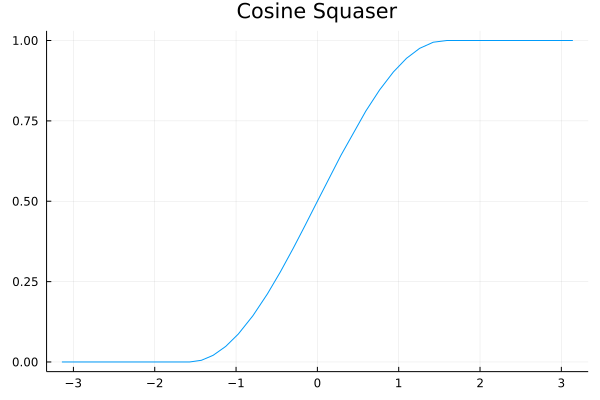
\includegraphics[width=.7\textwidth]{articulo_rrnn_aproximadores_universales/cosineSquaser.png}
        \caption{Función \textit{cosine squaser}}
        \label{fig:cosine_squaser}
    \end{figure}

    Se tiene pues que para cualquier $\lambda \in \left[ \frac{-\pi}{2}, \frac{\pi}{2}\right]$

    \begin{equation}
        2 F(\lambda)-1 = \cos \left( \lambda - \frac{\pi}{2}\right)
    \end{equation}

    Que haciendo $\mu = \lambda - \frac{\pi}{2}$ resulta que para cualquier
    $\mu \in [-\pi, 0]$
    \begin{equation}
        \cos(\mu) = 2 F \left(\mu + \frac{\pi}{2} \right)  -1 
    \end{equation}

    Además, puesto que $F(\mu + 2 \pi M) = 1$ para todo $\mu \in [-M, M] \supset [-\pi, 0]$ tenemos que
    para cualquier $\mu \in [-\pi, 0]$
    \begin{equation}
        \cos(\mu) = 2 F \left(\mu + \frac{\pi}{2} \right)  - F(\mu + 2 \pi M) 
    \end{equation}

    \begin{figure}[h]
        \centering
        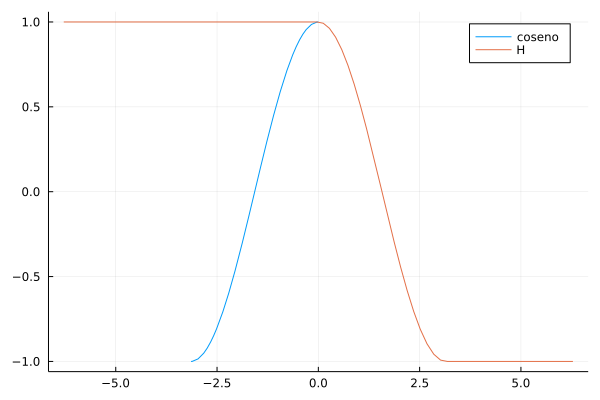
\includegraphics[width=.7\textwidth]{articulo_rrnn_aproximadores_universales/H_menos_pi_0.png}
        \caption{Comparativa $H_{[-\pi, 0]}$ con la función coseno real. }
        \label{fig:coseno_vs_H_menos_pi_cero}
    \end{figure}

    De manera generalizada denotaremos como $H_{[M_1,M_2 ]}$ a la función 
     existe $H_{[M_1,M_2 ]} \in \sum(F)$ 
    tal que para todo elemento $\lambda \in [M_1, M_2]$ se cumpla que 
    \begin{equation}
        H_{[M_1,M_2 ]}(\lambda) = \cos(\lambda)
    \end{equation}

    Por tanto $H_{[-\pi, 0]}$ viene definida como  
    \begin{equation}
        H_{[-\pi, 0]} = 2 F \left(\mu + \frac{\pi}{2} \right)  - F(\mu + 2 \pi M) 
    \end{equation}

    Por la simetría de la función coseno resulta que 
    para todo $\mu \in [0, \pi]$
    \begin{equation}
        \cos(\mu) = \cos(-\mu) = H_{[-\pi, 0]}(-\mu)
    \end{equation}
    \begin{figure}[h]
        \centering
        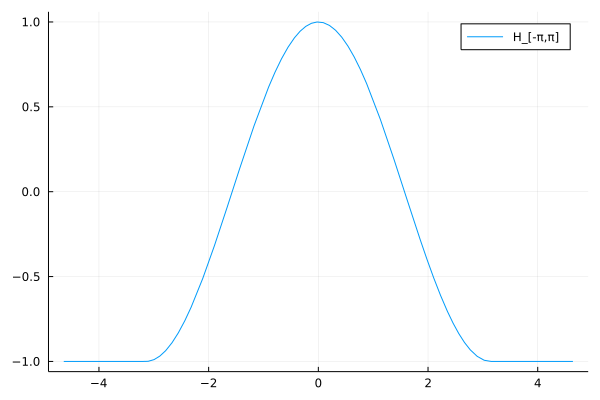
\includegraphics[width=.7\textwidth]{articulo_rrnn_aproximadores_universales/H_menos_pi_mas_pi.png}
        \caption{Función $H_{[-\pi, \pi]}$. }
        \label{fig:H_menos_pi_mas_pi}
    \end{figure}

    Así pues podemos definir 
    \begin{equation}
        \begin{split}
            H_{[-\pi, \pi ]}(\mu) &= H_{[-\pi, 0]}(\mu) + H_{[-\pi, 0]}(-\mu) - 1 \\
            &= H_{[-\pi, 0]}(\mu) + H_{[-\pi, 0]}(-\mu) - F(\mu + 2 \pi M). 
        \end{split} 
    \end{equation}  

    Por ser el coseno una función periódica es fácil ver que 
    considerando un natural $N$ que satisfaga que $2 \pi N \geq M$
  
    \begin{equation}
    \begin{split}
        H_{[-2\pi N, 2 \pi N]} (\lambda) = 
        \sum_{i=1}^N (H_{[-\pi, \pi ]}(\lambda + 2 \pi i) +1) 
        + H_{[-\pi, \pi ]}(\lambda)  \\
        - \sum_{i=1}^N (H_{[-\pi, \pi ]}(- \lambda + 2 \pi i - \pi) +1),
    \end{split}
\end{equation}
\begin{equation}
    \begin{split}
        H_{[-2\pi N, 2 \pi N]} (\lambda) 
        =  H_{[-\pi, \pi ]}(\lambda) + 
        \sum_{i=1}^N (
            H_{[-\pi, \pi ]}(\lambda + 2 \pi i)
            - 
            H_{[-\pi, \pi ]}(- \lambda + 2 \pi i - \pi)
        ) .         
    \end{split}
    \end{equation}

      % Ejemplos de la función H final
      \begin{figure}[h]
        \centering
        \begin{subfigure}[b]{0.45\textwidth}
            \centering
            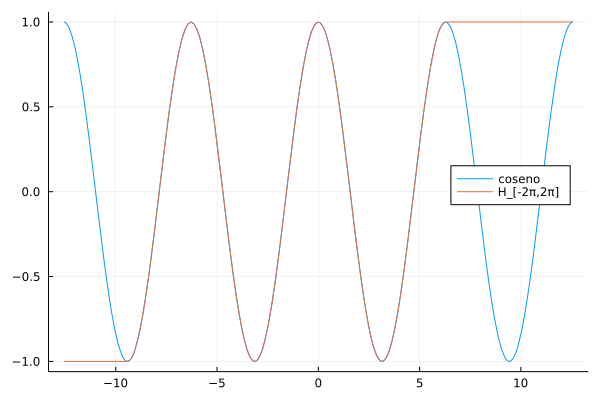
\includegraphics[width=\textwidth]{articulo_rrnn_aproximadores_universales/H_[-2π,2π].png}
            \caption{Función $H_{[-2\pi, 2\pi]}$ con $N=1$.}
            \label{fig:H_con_M}
        \end{subfigure}
        \hfill
        \begin{subfigure}[b]{0.45\textwidth}
            \centering
            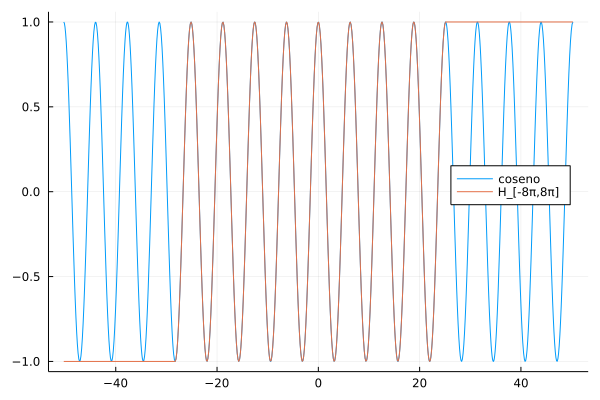
\includegraphics[width=\textwidth]{articulo_rrnn_aproximadores_universales/H_[-8π,8π].png}
            \caption{Función $H_{[-8\pi, 8\pi]}$ con $N=4$. }
        \end{subfigure}
        \hfill
        \caption{Ejemplos de funciones $H_{[-M, M]}$}
    \end{figure}

    Está claro que por ser $2 \pi N \geq M$ la función $H_{[-M, M]}$ será la restricción de la anterior, es decir: 

    \begin{equation}
        H_{[-M, M]} = H_{[-2\pi N, 2 \pi N]_{|[-M, M]}}.
    \end{equation}

    
    Así definida $H_{[-2\pi N, 2 \pi N]}$
    pertenecerá a $\sum(F)$ o lo que es de nuestro interés, estará 
    formada por una combinación finita, supongamos que $K$, 
    sumas y restas finita de $F \circ A_i$ con $A_i$ una función afín. 
    Por ser $F$ una función de activación continua gracias al
    lema \ref{lema:a_2_paso_previo_denso}, 
    existirá $W_{ \frac{\epsilon}{k}} \in \sum(\psi)$ tal que 
    podremos acotar $|F - W_{ \frac{\epsilon}{k}} | < \frac{\epsilon}{k}$ en todo $\R$.

    Además, como las transformaciones afines $A_i$ solo son traslaciones,
    para cada $i \in \{1,..K\}$ se cumple que 
     $W_{ \frac{\epsilon}{k}} \circ A_i \in \sum(\psi)$ y se mantiene que 
    \begin{equation}
        |F \circ A_i - W_{ \frac{\epsilon}{k}} \circ A_i | < \frac{\epsilon}{k}. 
    \end{equation}


    Recopilemos pues, tenemos que para $2\pi N \geq M$ y en el dominio $\lambda \in [-M, M]$: 
    \begin{equation}
        H_{[-M, M]} (\lambda) = 
        H_{[-2\pi N, 2 \pi N]}(\lambda) = 
        \sum_{i=1}^k \alpha_i F( A_i(\lambda)) \quad \alpha_i \in \{-1,1\}.
    \end{equation}
    fijando tales $\alpha_i \in \{-1,1\}$ y las traslaciones $A_i$ definimos 
    \begin{equation}
        \cos_{M, \epsilon}(\lambda) = \sum_{i=1}^k 
        \alpha_i  W_{ \frac{\epsilon}{k}}(A_i(\lambda)). 
    \end{equation}

    De esta manera, para cualquier $\lambda \in [-M, M]$

    \begin{equation}
        \begin{split}
            |\cos_{M,\epsilon}(\lambda) - \cos(\lambda)| 
            &= |\cos_{M,\epsilon}(\lambda) - \cos(\lambda) \pm  H_{[- M, M]}(\lambda)| \\
            &\leq
            |\cos(\lambda) -  H_{[- M, M]}(\lambda)|
            + 
            | \cos_{M,\epsilon}(\lambda) -  H_{[- M, M]}(\lambda)|  \\
            &\leq  0 
            + | \cos_{M,\epsilon}(\lambda) -  H_{[- M, M]}(\lambda)| \\
            & \leq  \sum_{i=1}^k 
            |  W_{ \frac{\epsilon}{k}}(A_i(\lambda)) 
            -
            F( A_i(\lambda))
             | \\
             & <   \sum_{i=1}^k \frac{\epsilon}{k} = \epsilon .
        \end{split}
    \end{equation}

    Dando con esto por concluida la demostración. 
 
\end{proof}

%Lema 4.A
\begin{lema}
    Sea $g(\cdot) = \sum_{j=1}^q \beta_j \cos(A_j(\cdot))$ con 
    $A_j \in A^r$. 
    Para cualquier función de activación $\psi$, 
    cualquier compacto $K \subset \R^r$
    y cualquier $\epsilon > 0$
    existe $f \in \sum^r(\psi)$ para el cual se cumple que 
    \begin{equation}
        \sup_{x \in K} 
        |g(x) - f(x)| < \epsilon.
    \end{equation}
\end{lema}

%Lema A.5 
\begin{lema}
    Para cualquier función de activación $\psi$ se tiene que 
    $\rrnn$ es uniformemente denso en compactos de $C^r.$
\end{lema}

% Teorema 2.4
\begin{teorema}
    Para cualquier función de activación $\psi$, $r \in \N$ y
    medida de probabilidad $\mu$ o $(\R^r, B^r)$, 
    se tiene que $\rrnn$ es uniformemente denso en compactos
    en $\fC$ y denso en $\fM$ de acorde a la distancia $\dist$. 
\end{teorema}
% !TeX root = ../../tfg.tex
% !TeX encoding = utf8
%
%***************************************************************
% Contenido del artículo 4: Colorario 2.1
%***************************************************************

% Resultado de teoría de la medida 
Trataremos ahora de generalizar la tesis expuesta en 
 el teorema \ref{teo:2_4_rrnn_densas_M} sobre las funciones medibles. 
 Para ello recordaremos el teorema de Lusin.
% Teorema de Lusin 
\begin{teorema}[Teorema de Lusin] \label{teo:Lusin}
    Si $\mu$ es una medida regular de Borel, $E$ un conjunto de medida finita 
    y $f$ una función medible en $E$ entonces
    para cualquier $\epsilon > 0$ existirá un conjunto compacto 
    $K$ en $E$ tal que $\mu(E \setminus C) \leq \epsilon$ y donde $f$ es continua en $K$. 
\end{teorema}
\begin{proof}
    Demostración en páginas 242 y 243 de \cite{nla.cat-vn1819421}.
\end{proof}  

Notemos los puntos clave de este teorema, nos va a permitir \textit{trabajar} con una función medible como si fuera continua en un compacto
todo lo parecido a $\R^r$ como se quiera. 
 
\begin{teorema}(Caracterización de normalidad de Tietze)\label{teo:Tietze}
    Sea $X$ un espacio Hausdorff. Son equivalentes las siguientes afirmaciones: 
    \begin{enumerate}
        \item $X$ es normal.
        \item Para cada conjunto cerrado $A \subset X$ y para cualquier función continua 
        $f: A \longrightarrow \R$, $f$ admite una extensión continua $F:X \longrightarrow \R.$
        Además, si para todo $a \in A$ se cumple que $|f(a)| < c \in \R$, se puede elegir $F$
        de tal forma que satisfaga que $|F(x)| < c$ para todo $x\in X.$ 
    \end{enumerate}
    (Demostración en páginas 149-151 de \cite{james1966topology})
\end{teorema}

Como el ambiente actual en el que estamos trabajando 
es el espacio $(\R^r, \mathcal{T})$ que sabemos que es normal y puesto que es habitual que nuestras funciones estén definidas
en  compactos de $\R^r$, las podremos extender a $\R^r$. 


% Corolarios del artículo 
% Corolario 2.1
\begin{corolario} \label{cor:2_1}
    Para cada función $g \in \fM$ existe un subconjunto compacto 
    $K$ de $\R^r$ y $f \in \rrnn$ tal que para cualquier 
    $\epsilon > 0$ se tiene que 
    $\mu(K) > 1- \epsilon$ y para cada $x \in K$ tenemos que 
    \begin{equation}
        |f(x) - g(x) | < \epsilon,
    \end{equation}
    independientemente de la función de activación $\psi$, dimensión $r$ o medida $\mu$. 
\end{corolario}

    \marginpar{
    \textcolor{dark_green}{
        \textbf{Idea intuitiva corolario \ref{cor:2_1}}
    }
    }
    \marginpar{
    Este teorema corrige la carencia sobre la precisión del error que describíamos en la idea intuitiva del teorema \ref{teo:2_4_rrnn_densas_M}. Podemos encontrar una red neuronal que aproxime cualquier función medible que queramos en todos los puntos del espacio que queramos.
    }

    
\begin{proof}
    Sea $\epsilon > 0$ fijo pero arbitrario.  Gracias al teorema de Lusin \ref{teo:Lusin}
    existe un subconjunto compacto $K \subset \R^r$ de medida
    $\mu(K) > 1 - \epsilon$ donde la restricción  $g_{|K}$ es continua. 

    Por otra parte, en virtud de la caracterización de Tietze 
    \ref{teo:Tietze}, 
    por estar $g_{|K}$ definida en un compacto, admite una 
    extensión continua $G:\R^r \longrightarrow \R$ tal que 
    \begin{equation}
        \begin{split}
            G_{|K} = g_{|K} .
        \end{split}
    \end{equation}

    Por ser $G$ continua en un compacto, por la densidad de las redes neuronales en compactos en $\fC$(lema \ref{lema:A_5_uniformemente_denso_compactos} ) se tiene que existirá 
     $f \in \rrnng$ tal que 
    \begin{equation}
        \sup_{x \in K} |G(x) - f(x)| < \epsilon.
    \end{equation}

    Por lo que podemos afirmar que para todo $x \in K$
    \begin{equation}
        |f(x) -g(x)| 
        \leq 
        | f(x) -G(x)| + |G(x) -g(x)|
        < \epsilon + 0 = \epsilon
    \end{equation}
    como queríamos probar.
\end{proof}



% !TeX root = ../../tfg.tex
% !TeX encoding = utf8
%
%***************************************************************
% Contenido del artículo 5: Colorarios LP
%***************************************************************
\section{Generalización a espacios $L_p$}  
\label{ch04:espacios-Lp}
Hasta ahora habíamos considerado el espacio de funciones continuas 
$\fC$ 
como subespacio dentro del espacio de funciones medibles $\fM$. 
Sin embargo, ser continua es una hipótesis muy estricta ya que existe una amplia gama de subespacios que contienen al de 
las funciones continuas y están contenidos en el de funciones medibles. 
Es por ello que vamos a realizar una generalización de los teoremas
para espacios $L_p$. De manera intuitiva estos espacios nos van a 
permitir considerar funciones que no necesariamente sean continuas
y que incluso no están acotadas. 

 % Nota intuitiva sobre la definición  LP
 \normalmarginpar
 \marginpar{\maginLetterSize\raggedright
 \iconoAclaraciones \textcolor{dark_green}{ 
     \textbf{Idea intuitiva de espacio $L_p$}
 }
 }
 \marginpar{\maginLetterSize
 Con esta definición lo que se trata es de considerar funciones 
 que tomen un valor real en la mayoría de sus puntos.
 Ya que la integral no varía su valor si se aplican cambios puntuales. 
 }
\begin{definicion}[Espacios Lp]
    Se llama espacio $L_p(\R^d, \mu)$ o simplemente $L_p$ al conjunto 
    de funciones $f \in \fM$ tales que 
    \begin{equation}
        \int |f(x)|^p d\mu < \infty. 
    \end{equation}  
Se define la norma de $L_p$ como 
\begin{equation}
    \| f\|_p 
    =
    \left(\int |f(x)|^p d\mu \right)^\frac{1}{p}
\end{equation}
y la distancia asociada al espacio $L_p$ se define como 
\begin{equation}
    \rho_p(f,g) = \| f-g\|_p.
\end{equation}
\end{definicion}


% Corolario 2.2
\begin{corolario}\label{corolario:2_2_rrnn}
    Si existe un subconjunto compacto $K$ en $\R^d$ de medida
    $\mu(K) =1$ entonces $\rrnn$ es $\dlp$-denso en $L_p(\R^d, \mu)$
    para cualquier $p \in [1,\infty)$, independientemente de 
    $\psi$, $d$ o $\mu$.
\end{corolario}

% Nota intuitiva sobre el corolario 2.2
\marginpar{\maginLetterSize\raggedright
    \iconoAclaraciones \textcolor{dark_green}{ 
        \textbf{Idea intuitiva corolario \ref{corolario:2_2_rrnn}}
    }
}
\marginpar{\maginLetterSize
Se prueba que las redes neuronales son capaces de aproximar 
cualquier función de la clase recién introducida.
}


\begin{proof}
    Se quiere probar que para cualquier $g \in L_p$ y 
    $\varepsilon >0$ existe $f \in \rrnn$ tal que 
    \begin{equation}
        \dlp(f,g) <\varepsilon.
    \end{equation}   
    
    Por pertenecer $g$ a $L_p$ existe una constante $M$ real positiva
    lo suficientemente grande 
    tal que si definimos la función $h =g 1_{|g|<M}$ esta satisface 
    que
    \begin{equation}\label{eq:corolario_2_2:h_compacto}
        \dlp(g,h) < \frac{\varepsilon}{3}.
    \end{equation}
    
    Además como $h$ es una función acotada de $L_p$, podemos encontrar
    una función $s$ continua que es límite de una sucesión de
    funciones simples 
    ( pag 241-242,  teoremas 55C y 55D \cite{nla.cat-vn1819421})
    y la cual cumple que 

    \begin{equation}\label{eq:corolario_2_2:s_continua}
        \dlp(h,s) < \frac{\varepsilon}{3}.
    \end{equation}

    Por el teorema \ref{teo:2_4_rrnn_densas_M}, al estar en un compacto $K$ y por ser $\rrnn$ uniformemente
    denso en compactos hay una $f \in \rrnn$ la cual cumple que
    \begin{equation}
        \sup_{x \in K} |f(x) -s(x)|^p 
        <
         \left( \frac{\varepsilon}{3}\right) ^p.
    \end{equation}
    
    Y por hipótesis $\mu(K) =1$ y definición de la distancia $\dlp$ 
    se tiene la siguiente desigualdad: 

    \begin{equation} \label{eq:corolario_2_2:cota_rrnn}
        \dlp(f,s) = 
        \left(\int |f(x) - s(x)|^p d\mu \right)^\frac{1}{p}
        \leq 
        \left(\int  \left( \frac{\varepsilon}{3}\right) ^p d\mu \right)^\frac{1}{p}
        = \left( \mu(K)  \left(\frac{\varepsilon}{3} \right)^p\right) ^\frac{1}{p}
        = \frac{\varepsilon}{3}.
    \end{equation}

    Gracias a la desigualdad triangular y las desigualdades
    (\refeq{eq:corolario_2_2:cota_rrnn}),
    (\refeq{eq:corolario_2_2:h_compacto}) y 
    (\refeq{eq:corolario_2_2:s_continua})
    tenemos
    \begin{equation}
        \dlp(f,g) 
        \leq
            \dlp(f,s)
            +\dlp(s,h)
            + \dlp(h,g)
        < 
        \frac{\varepsilon}{3} + \frac{\varepsilon}{3} + \frac{\varepsilon}{3}
        = \varepsilon.
    \end{equation}
Probando con ello lo buscado. 
\end{proof}  

% Corolario 2.3
\begin{corolario}\label{corolario:2_3_medida_probabilidad}
    Si $\mu$ es una medida de probabilidad en $[0,1]^d$
    entonces 
    $\rrnn$ es $\dlp$-denso en 
    $L_p([0,1]^d, \mu)$ para todo $p \in [1, \infty)$,
    independientemente de $\psi, d, \mu$. 
\end{corolario}

% Nota intuitiva sobre el corolario 2.3
\marginpar{\maginLetterSize\raggedright
    \iconoAclaraciones \textcolor{dark_green}{ 
        \textbf{Idea intuitiva corolario 
        \ref{corolario:2_3_medida_probabilidad}}
    }
}
\marginpar{\maginLetterSize
    A diferencia que con el corolario \ref{corolario:2_2_rrnn},
aquí se afirma que las redes neuronales son capaces de aproximar 
cualquier función de la clase recién introducida cuyo dominio parta de $[0,1]^d$, es decir \textbf{se está concretando los valores de entrada que pueden tomar las funciones}.
}


\begin{proof}
    Es consecuencia directa del corolario previo \ref{corolario:2_2_rrnn}
    donde para este caso particular $K = [0,1]^d$ un compacto
    de $\R^d$
    que cumple que $\mu(K) = 1.$
\end{proof}

%Corolario 2.4 
\begin{corolario} \label{corolario:2_4_conjunto_finito}
    Sea $\mu$ una medida, que para
    un conjunto finito de puntos $O$ cumple que $\mu(O)=1$, 
    entonces, para cualquier función medible $g \in \fM$
    y sea cual sea $\varepsilon >0$ 
    existe $f \in \rrnn$ la cual cumple que 
    \begin{equation}
        \mu\{ 
            x:
            |f(x) - g(x)| 
            < \varepsilon
        \}
        = 1.
    \end{equation}

\end{corolario}
\begin{proof}
    Por el teorema \ref{teo:2_4_rrnn_densas_M} existe 
    $f \in \rrnn$ tal que para cualquier 
    $\varepsilon_1, \varepsilon_2 >0$ se cumple que 
    $\mu \{x: |f(x) - g(x)| > \varepsilon_1\} < \varepsilon_2.$
    Sea $O$ el conjunto de puntos tal que $\mu(O) = 1.$
    Por ser finito $O$ podemos encontrar
    \begin{equation} \label{eq:2_4:definición_epsilon}
        \delta = \min_{x \in O} \{ 
            \mu(x) : \mu(x)>0
        \}. 
    \end{equation}

    Sin pérdida de generalidad tomamos $\varepsilon < \delta$ y entonces
    para  que la $f$ fijada cumpla que
    \begin{equation}
        \dist(f,g) = \varepsilon
    \end{equation}
    debe de cumplirse que 
    \begin{equation}
        \dist(f,g) =  \inf 
        \{
           \varepsilon_1 > 0:
           \mu\{ 
            x:
            |f(x) - g(x)| 
            > \varepsilon_1
        \}
        < \varepsilon_1
        \} 
        = \varepsilon,
    \end{equation}
    pero por cómo tomamos $\varepsilon$ en (\refeq{eq:2_4:definición_epsilon}) se
    tiene que $\mu\{ 
        x:
        |f(x) - g(x)| 
        > \varepsilon
    \} = 0.$
    Por lo que acabamos de probar, como queríamos, que 
    \begin{equation}
        \mu\{ 
            x:
            |f(x) - g(x)| 
            < \varepsilon
        \}
        = 1.
    \end{equation}
\end{proof}

Nótese que con este corolario lo que se está indicando es que dado
un conjunto finito y sus respectivas imágenes, se puede encontrar una red neuronal que para tales puntos \textit{devuelva} el valor exacto. 
%Nota aclarativa sobre la relevancia del corolario
\marginpar{\maginLetterSize
    \iconoAclaraciones \textcolor{dark_green}{     
        \textbf{
            Relevancia práctica del corolario 
            \ref{corolario:2_5_función_Booleana}
        }
    }
     
    Este resultado nos permite \textbf{aproximar funciones que actúen como clasificadores discretos}. Por ejemplo sea $g$ como una función que dada una imagen $x$ indica si hay un perro haciendo valer $g(x)=1$ y en caso contrario $g(x)=0$.
      
}

%Nota aclarativa sobre la implementación del corolario
\marginpar{\maginLetterSize
    \textcolor{red}{    
        \textbf{
            Observación sobre la implementación
            del corolario
            \ref{corolario:2_5_función_Booleana}
        }
    }
    
    El resultado nos   indica que podemos obtener una red neuronal $h$ que aproxime tal clasificador, 
    pero \textbf{tal red neuronal no necesariamente tomará valores discretos}, es decir,
     pudiera darse el caso en que las imágenes 
     a un rango, por ejemplo: 
     $$h( \{ x : g(x)=0 \})  \subset [-0.2,0.3]$$ 
     y que 
     $$h(\{ x : g(x)=1 \})  \subset [0.9,1.2],$$ 
     por lo que se pone de manifiesto en este
      resultado, 
     que en caso de requerirse
      de una salida completamente
     discreta debería de componerse 
     con otra función $\theta$ 
     tal que 
     $$\theta \circ h(\{ x : g(x)=0 \})=0$$ y 
     $$\theta \circ h(\{ x : g(x)=1 \})=1$$.
    
}

\begin{definicion}[Función Booleana]
    Decimos que una función es Booleana si su dominio es 
    $\{0,1\}^d$  para algún $d \in \N \setminus \{0\}$
    y su codominio es $\{0,1\}$. Es decir,
    \begin{equation}
      f:\{0,1\}^d \longrightarrow \{0,1\}.
    \end{equation}
\end{definicion}

Ejemplos conocidos son la función 
$or: \{0,1\}^d \longrightarrow \{0,1\}$  que vale 
uno si alguno de su entrada es uno y la función 
$and: \{0,1\}^d \longrightarrow \{0,1\}$
que se define como $and(x_1, \ldots, x_d) = \prod_{i=1}^d x_i.$

% Corolario 2.5  
\begin{corolario}\label{corolario:2_5_función_Booleana} 
    Para cada función Booleana 
    $g: \{0,1\}^d \longrightarrow \{0,1\}$
     y 
    cada $\varepsilon >0$ existe una red neuronal
    $f \in \rrnn$ tal que 
    \begin{equation}
        \max_{x \in \{ 0,1\}^d} |g(x) - f(x)|
        < \varepsilon.
    \end{equation}
\end{corolario}



\begin{proof}
    Se define la función $\mu : \R^d \longrightarrow [0,1]$ de forma que 
    \begin{equation}
        \mu(x) = 
      \left \{
    \begin{aligned}
      \frac{1}{2^d} \quad &\text{ si } x \in \{0,1\}^d \\
      0 \quad & \text{ si } x \notin \{0,1\}^d 
    \end{aligned}
  \right .
    \end{equation}

    Se tiene que $\mu$ es una medida ya que cumple que 
    \begin{enumerate}
        \item Hipótesis de acotación: $0 \leq \mu(A) \leq 1$ para $A \in \mathcal{P}(\R^d).$
        \item La probabilidad del vacío es nula y la del  total es la unidad. 
        \item La probabilidad de la unión es la suma de la probabilidades. 
        \begin{equation}
            P\left(
                \cup_{i=1}^n A_i
            \right)
            = \sum_{i=1}^n P(A_i).
            \quad
            \forall A_i \in  \mathcal{P}(\R^d).
        \end{equation}
    \end{enumerate}  

    Como la cardinalidad de $\{0,1\}^d$ es $2^d$
    podemos aplicar el corolario \ref{corolario:2_4_conjunto_finito}
    y entonces sabemos que  existe $f\in \rrnn$ tal que 
    \begin{equation}
            \mu\{ 
                x:
                |f(x) - g(x)| 
                < \varepsilon
            \}
            = 1,
    \end{equation} 
    es decir que 
    \begin{equation}
        \max_{x \in \{ 0,1\}^d} |g(x) - f(x)|
        < \varepsilon
    \end{equation}
    como queríamos probar. 
\end{proof}


% Lemas propios  previos al teorema 2.5
\begin{lema} \label{lema:propio_1_antes_teorema_2_5}
    Si una función de activación  $\psi$ alcanza el cero y el uno, esto es 
    si existen dos constantes reales $M_1, M_2$ 
    tales que 
    \begin{equation}
        \psi(M_1) = 0 \text{ y } \psi(M_2)=1
    \end{equation}
    entonces existe una constante real positiva $M$ tal que 
    \begin{equation}
        \psi(-M) = 1- \psi(M) = 0.
    \end{equation}
\end{lema}
\begin{proof}
Sea $M = \max \{|M_1|,|M_2|\}$ y por ser $\psi$ una función de activación sabemos que
es no decreciente y que su imagen pertenece al intervalo $[0,1].$

Por tanto
\begin{align}
      0 &\leq \psi(-M) \leq \psi(M_1) = 0 \quad \text{ luego } \quad \psi(-M) = 0, \\
      1 &\geq \psi(M) \geq \psi(M_2) = 1 \quad \text{ luego } \quad\psi(M) = 1.
\end{align}

Gracias a estas desigualdades es fácil ver que 
\begin{equation}
    \psi(-M) = 1 - \psi(M) = 0
\end{equation}
como queríamos probar. 
\end{proof}   

Es interesante percatarse de que de no exigirse la hipótesis de 
que $\psi$ alcanza el cero y el uno no puede 
asegurarse la igualdad demostrada. Pongamos como ejemplo la siguiente función de activación

\begin{equation}
    \psi(x)= \left\{ \begin{array}{lcc}
        0 &   si  & x \leq 0 \\
        \frac{| x |}{1+ | x |}&  si & 0< x. 
        \end{array}
    \right. 
\end{equation}


% Otro lema propio antes de probar el teorema 2.5
\begin{lema}\label{lema:previo_propio_2_al_teorema_2_5}
    Dado un conjunto finito de vectores $\Lambda \subset \R^d$ con 
    $d$ natural positivo. 
    Existe un vector $p \in \R^d$ que satisface que 
    para cualesquiera $x,y \in \Lambda$ diferentes 
    \begin{equation}
        p \cdot(x-y) \neq 0.
    \end{equation}
\end{lema}
% Nota intuitiva sobre el Teorema 2.5
\marginpar{\maginLetterSize\raggedright
    \iconoAclaraciones \textcolor{dark_green}{ 
        \textbf{Idea clave teorema
        \ref{teorema:2_5_entrenamiento_redes_neuronales}}
    }
}
\marginpar{\maginLetterSize
   Podemos conseguir una red neuronal que \textit{valga} lo que queramos en un conjunto finito de puntos.
}
% Prueba lema propio antes de probar el teorema 2.5
\begin{proof}
    Si $n$ es el cardinal de $\Lambda$,
    consideramos el conjunto $U$ definido como la unión de 
    $n (n-1)$ hiperplanos de $\R^d$

    \begin{equation}
        U = \bigcup_{ 
            \substack{
                x,y \in \Lambda \\
                x \neq y
            }
        }
        \{ 
            p \in \R^d: p \cdot (x-y) = 0
        \}.
    \end{equation}

    Puesto que $\R^d$ no puede ser expresado como unión finita de hiperplanos,
    $U \subsetneq \R^d$ y por tanto existirá $p \in \R^d \setminus U$ tal que 
    \begin{equation}
        p \cdot(x-y) \neq 0 
        \text{ para cualesquiera }
         x,y \in \Lambda \text{ diferentes, }
    \end{equation}
    como queríamos probar. 
\end{proof}

% Nota intuitiva sobre la demostración del Teorema 2.5
\setlength{\marginparwidth}{\smallMarginSize}
\marginpar{\maginLetterSize\raggedright
    \iconoAclaraciones \textcolor{dark_green}{ 
        \textbf{Idea de la demostración del teorema
        \ref{teorema:2_5_entrenamiento_redes_neuronales}}
    }
}
\marginpar{\maginLetterSize
    {
  Es interesante reparar en que la demostración se basa
  en añadir una neurona por cada punto que queramos que tome
  un valor concreto, esa neurona se activará (es decir, no será nula) cuando la entrada $x$ \textit{sea mayor} que el valor que la activa $x_i$ y vale la diferencia con el valor anterior $x_{i-1}$, es decir $g(x_{i}) - g(x_{i-1})$, como el nodo $x_{i-1}$
  también se activará por ser menor, el término $g(x_{i-1})$ se suma a la salida de la red y así como una serie telescópica al final solo resultará el valor $g(x_i)$.
    }
}
\setlength{\marginparwidth}{\bigMarginSize}
% fin de la nota


% Teorema 2.5  
\begin{teorema}[Sobre el entrenamiento práctico de redes neuronales]
    \label{teorema:2_5_entrenamiento_redes_neuronales}
    Sea $ \Lambda = \{x_1, \ldots, x_n\}$ un conjunto de puntos distintos de 
    $\R^d$ y sea 
    $g: \R^d \longrightarrow \R$ una función arbitraria. 
    Si $\psi$ alcanza el cero y el uno, 
    entonces
    existe una red neuronal $f \in \rrnn$ con $n$
    neuronas ocultas tal que 
    \begin{equation}
        f(x_i) = g(x_i) \text{ para todo } i \in \{1, \ldots, n \}.
    \end{equation}
\end{teorema}

\begin{proof}
Con el fin de facilitar la comprensión dividiremos la demostración en dos casos, 
primero uno particular, cuando $d=1$ y después el caso general.

\textbf{Caso primero}

Suponemos que $\{x_1, \ldots, x_n\} \subset \R$ y tras renombrar 
podemos suponer que 
\begin{equation}
    x_1 < x_2 < \cdots < x_n. 
\end{equation}

Por alcanzar la función de activación $\psi$ el cero y el uno, 
gracias al lema  \ref{lema:propio_1_antes_teorema_2_5} existe una constante $M$ tal que $\psi(-M) = 1-\psi(M) = 0.$

Definiremos de manera recursiva la red neuronal buscada $f_n$.

% Nota nueva hipótesis de optimización del Teorema 2.5

\marginpar{\maginLetterSize\raggedright
     \iconoProfundizar \textcolor{blue}{
        \textbf{Nueva hipótesis de optimización}
    }
}
\marginpar{\maginLetterSize
    \textbf{
    El teorema 
        \ref{teorema:2_5_entrenamiento_redes_neuronales}
        nos brinda una heurística de inicialización de los pesos
        de una red neuronal.
    }
    La cual se tratará en la sección \ref{section:inicializar_pesos}.
\setlength{\marginparwidth}{\bigMarginSize}
 
}

\begin{itemize}
    \item Red neuronal $f_1$. 

Sea $A_1$ la función afín constante $A_1 = M.$
Fijamos $\beta_1 = g(x_1)$. 
De esta manera la red neuronal $f_1$ queda
definida como $f_1(x) = \beta_1 \psi(A_1(x)).$

\item Red neuronal $f_k$ con $1 < k \leq n$. 

Se define $A_{k}$ como la única función afín que cumple que 
\begin{equation}
    A_k(x_{k-1}) = -M \quad \text{y} \quad  A_{k}(x_k)= M.
\end{equation}
Fijamos $\beta_k = g(x_k) - g(x_{k-1})$. 
La red neuronal $f_k$ se calcula como 
\begin{equation}
    f_k(x) 
    = 
    \sum_{j=1}^k \beta_j \psi(A_j(x))
     = 
    (g(x_k)-g(x_{k-1})) \psi(A_k(x)) + f_{k-1}(x) .  
\end{equation}
Observemos que así construida se tiene que para cualquier
 $y > x_k$ la evaluación con la red neuronal resulta $f_k(y) = g(x_k).$
\end{itemize}

Veamos por inducción sobre $n$ que así definida para cualquier $1 \leq i \leq n$ se tiene que     
$f_n(x_i) = g(x_i)$. 
Además de que tiene un total de $n$ neuronas ocultas. 


\begin{itemize}
    \item Caso base, $n=1$. 
    \begin{equation}
        f_1(x_1)= \beta_1 \psi(A_1(x_1)) = g(x_1)\psi(M) = g(x_1).
    \end{equation}
    \item Supuesto que es cierto para $n-1$ veamos que lo es para $n$.      
    Evaluación de $x_n$
    \begin{align}
        f_n(x_n) 
        &= 
        (g(x_n) - g(x_{n-1}))\psi(A_n(x_n)) + f_{n-1}(x_n)
        \\
        & = (g(x_n) - g(x_{n-1}))\psi(M) + g(x_{n-1}) 
        \\
        & = (g(x_n) - g(x_{n-1})) + g(x_{n-1}) 
        \\
        & = g(x_n).
    \end{align}

Evaluación de $x_i$ con $1 \leq i < n$. 

Usando que $0 \leq \psi(A_n(x_i)) < \psi(A_n(-M)) = 0$ y la hipótesis de inducción se tiene que 
\begin{align}
    f_n(x_i) 
        &= 
        (g(x_n) - g(x_{n-1}))\psi(A_n(x_i)) + f_{n-1}(x_i)
        \\
        & = 0 + g(x_{i}) 
        \\
        &= g(x_i).
\end{align}
\end{itemize}

Acabamos de probar por inducción  que
$f_n(x) = g(x)$ para cualquier $x \in \Lambda$, lo que termina la demostración.

\textbf{Caso segundo}  

Se tiene para este caso que $\Lambda \subset \R^d$ con $d >1$. 
Seleccionamos $p \in \R^d$ cumpliendo que 
para cualesquiera $x,y \in \Lambda$ distintos 
$p(x-y) \neq 0$ (es posible de 
encontrar por el lema \ref{lema:previo_propio_2_al_teorema_2_5}).
Gracias a esta condición cada producto $p \cdot x$ con $x \in \Lambda$ es distinto y podemos establecer con ello una relación de orden, que tras 
renombrar los elementos de $\Lambda$ queda
\begin{equation}
    p \cdot x_1 < p \cdot x_2 < \cdots < p \cdot x_n,
\end{equation}
y como procedimos en el caso primero, definimos de manera
 recursiva la red neuronal $f_n$ buscada:

 \begin{itemize}
 \item Red neuronal $f_1$. 

Sea $B_1$ 
la función afín de $\R$ a $\R$ constante $B_1 = M.$
Fijamos $\beta_1 = g(x_1)$. 
De esta manera la red neuronal $f_1$ 
definida como $f_1(x) = \beta_1 \psi(B_1(p \cdot x)).$

\item Red neuronal $f_k$ con $1 < k \leq n$. 

Se define $B_{k}$ como la única función afín de $\R$ en $\R$ que cumple que 
\begin{equation}
    B_k(p \cdot x_{k-1}) = -M 
    \quad \text{y} \quad 
     B_{k}(p \cdot x_k)= M.
\end{equation}
Podemos definir entonces $A \in \afines$ por 
$A_k(x)=B_k(p \cdot x).$
Fijamos  también
$$\beta_k = g(x_k) - g(x_{k-1}).$$ 
La red neuronal $f_k$ se calcula como 
\begin{align}
    f_k(x) 
    = &
    \sum_{j=1}^k \beta_j \psi(B_j(p \cdot x))
     = 
    (g(x_k)-g(x_{k-1})) \psi(B_k(p \cdot x)) + f_{k-1}(x) \\
    \\
    & = 
    \sum_{j=1}^k \beta_j \psi(A_j(x))
    = 
   (g(x_k)-g(x_{k-1})) \psi(A_k(x)) + f_{k-1}(x).  
\end{align}
\end{itemize}

Así definida, la prueba por inducción es idéntica a la del caso primero y hemos encontrado por tanto la red neuronal $f_n$ buscada.
\end{proof}

\subsection{Reflexión sobre el número de neuronas} \label{subsection:reflexión_sobre_número_de_neuronas}

Ante la pregunta natural de 
\textit{¿cuántas neuronas son necesarias?} el 
recién probado teorema nos responde que 
si estamos entrenando con $n$ datos, con $n$ neuronas es suficiente para volver a reproducir esos datos. Pero esto carece de sentido a nivel práctico por los siguientes motivos. 

\subsubsection*{Naturaleza de los datos}  
Recordemos que el problema al que nos enfrentamos es el siguiente:
queremos ser capaces de predecir cierto fenómeno regido por $g$ una \textit{función} desconocida. 
Para ello tenemos un \textit{conjunto de muestras} 
compuestas por pares $(x, g(x))$, es decir, ante la situación $x$
hemos observado que el fenómeno se comporta como $g(x)$. Todo esta 
situación experimental puede producir incoherencias teóricas, como por ejemplo que se tengan dos muestras $(x_1, y_1), (x_2, y_2)$ 
tales que $x_1 = x_2$ pero $y_1 \neq y_2$ o que la medición contenga errores, es decir $(x, g(x)+\delta)$. 

Se podría paliar esta situación con un
 preprocesado de los datos. 

\subsubsection*{ Naturaleza de la regla subyacente}  

Supongamos que los datos de entrenamiento son perfectos. Existen infinitas aplicaciones 
que evalúan de la misma manera un conjunto finito de puntos. 
¿Cuáles tomar?

Podríamos, siguiendo el principio de economía de Ockham optar
por modelos que reduzcan el número de neuronas, pero entonces la 
pregunta sería  ¿qué número mínimo de neuronas serían necesarios para representar el modelo? 
Una solución sería tomar un número de neuronas menor que el tamaño del conjunto de 
entrenamiento y utilizar esa \textit{redundancia} de datos para 
\textit{afinar}. 

\subsubsection*{Coste computacional inasumible}  
Supongamos que los datos son idílicos, el modelo se conoce y se establece un tamaño de datos de entrenamiento suficiente y
un número de neuronas acorde  ¿podríamos asumir el coste computacional?


% !TeX root = ../../tfg.tex
% !TeX encoding = utf8
%
%***************************************************************
% Contenido del artículo 5: Generalización a multi-output 
%***************************************************************
\section{Generalización para \textit{multi-output neural networks}}
\label{ch04:salida-varias-dimensiones}
En las secciones anteriores se han provisto resultados para redes 
neuronales de salida real. Vamos a generalizar los resultados vistos
para ser capaces de aproximar funciones continuas o medibles 
de $\R^d$ a $\R^s$ con $d,s \in \N.$

Denotaremos por $\fCC$ al conjunto de funciones continuas definidas de $\R^d$ a $\R^s$ y al de funciones medibles de 
$\R^d$ a $\R^s$  por $\fMM.$ 
La distancia asociada a estos espacios se define como 
\begin{equation}
    \rho_{\mu}^s(f,g) 
    =
    \sum_{i=1}^s \dist(f_i, g_i).
\end{equation}

Con la siguiente definición buscamos abstraer el modelo de una red neuronal de una capa oculta y salida múltiple.
\begin{figure}[h]
    \centering
    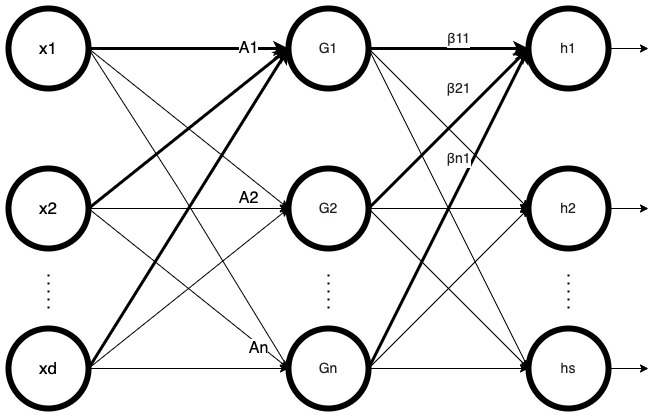
\includegraphics[width=.9\textwidth]{articulo_rrnn_aproximadores_universales/Red-Neuronal-blanco-negro-varias-salidas.jpg}
    \caption{Ejemplo de red neuronal de una capa oculta con $n$ nodos, de dimensión de entrada $d$ y salida $s$.}
    \label{fig:red neuronal-r-h-s}
\end{figure}

Nótese que los vectores $(w_{0i},w_{1 i}, \ldots, w_{r i})$ representan a la aplicación afín 
$A_i((x_1, x_2, \ldots x_r)) = w_{0i} + \sum_{j=1}^d w_{ji} x_j$
con $i \in \{1,\ldots, h\}$ . 

\begin{definicion}[Abstracción de una red neuronal con una capa oculta y múltiple salida] 
    Para cualquier función Borel medible $G$, definida de $\R$ a $\R$ y cualquiera naturales positivo
    $d,s \in \N$ se define a la clase de funciones $\rrnnmc$ como 
    \begin{equation}
        \begin{split}
        \rrnnmc = 
        \{ 
            & h: \R ^d \longrightarrow \R^s, h= (h_1, h_2, \ldots, h_s)  / \quad 
            \\ &
            \text{ con } h_i : \R ^d\longrightarrow \R, 
            h_i(x)=\sum_{j = 1} ^{n_i} (
            \beta_{j i} G(A_{j}(x)) \quad i \in \{1,2,\ldots, s\}, \\
            & x  \in \R ^d, \beta_{j i} \in \R, A_{j}\in \afines,n_i \in \N, i \in \{1,\ldots, s\} 
        \}.
        \end{split}
    \end{equation}
\end{definicion}

\iconoAclaraciones \textcolor{dark_green}{ Observación: }

% Comentario 
\marginpar{\maginLetterSize
    \iconoAclaraciones \textcolor{dark_green}{     
        \textbf{
        Por qué se ha destacado la observación
        }
    }
    Se destaca tal observación para remarcar que una 
    red neural con salidas en varias dimensiones tiene
    una definición mucho más estricta y que podría dar a confusión.
    
}

Es interesante apreciar que se tiene que 
    \begin{equation} \label{eq:diferencia_conjuntos_multicapa}
        \begin{split}
        \rrnnmc \subsetneq
        \{ 
            & h: \R ^d \longrightarrow \R^s, h= (h_1, h_2, \ldots, h_s)  / \quad 
            \\ &
            h_i \in \rrnn \quad \forall i \in \{1, \ldots, s\}
        \}.
        \end{split}
    \end{equation}
    aunque como veremos en el corolario \ref{corolario:2_6} $\rrnnmc$ es un espacio denso en el conjunto que acabamos de presentar. 
    Si tenemos presente que de acorde a nuestras definiciones una red neuronal $h_i$ viene determinada por un conjunto de funciones afines $A^{(i)}_j$  y escalares $\beta^{(i)_j}$, se daría la igualdad en \refeq{eq:diferencia_conjuntos_multicapa} si imponemos que para cualquier par de redes neuronales $h_k, h_j$ se satisface que $A^{(k)}_i = A^{(j)}_i$. 


No es difícil pensar que su versión generalizada sea: 

\begin{definicion} 
    Dadas las mismas hipótesis que en la definición anterior, se define la siguiente clase de funciones como 
    \begin{equation}
        \begin{split}
            \sum \prod^{d, s}(G) 
            = 
        \{ 
            & f: \R ^d \longrightarrow \R^s, f= (f_1, f_2, \ldots , f_s)  / \quad 
            \\ &
            \text{ con } f_i : \R ^d\longrightarrow \R, 
            f_i(x)=\sum_{j = 1} ^h 
            \left(
            \beta_{j i} \prod_{k=1}^{l_{j i}} G(A_{j i}(x))
            \right)
             \quad i \in \{1,2,\ldots, s\}, \\
            & x \in \R ^d, \beta_{j i} \in \R, A_{j i}\in \afines; h,l_{j i} \in \N 
        \}.
        \end{split}
    \end{equation}
\end{definicion}


% Corolario 2.6  
\begin{corolario}\label{corolario:2_6}
    Los teoremas 
    \ref{teorema:2_3_uniformemente_denso_compactos},
    \ref{teo:2_4_rrnn_densas_M} 
    y los corolarios
    \ref{cor:2_1}, 
    \ref{corolario:2_2_rrnn},
    \ref{corolario:2_3_medida_probabilidad},
    \ref{corolario:2_4_conjunto_finito}
    y 
    \ref{corolario:2_5_función_Booleana}
    permanecen válidos si se sustituye $\rrnn$ por $\rrnnmc$
    ,$\rrnng$ por $\rrnngmc$, 
    los espacios de funciones continuas y medibles por $\fCC$ y $\fMM$ respectivamente.
\end{corolario}

% Nota intuitiva sobre el Corolario 2.6
\marginpar{\maginLetterSize\raggedright
    \iconoAclaraciones \textcolor{dark_green}{ 
        \textbf{Idea clave corolario
        \ref{corolario:2_6}}
    }
}
\marginpar{\maginLetterSize
   En esencia, todos los resultados probados hasta ahora para redes 
   neuronales con salida real de dimensión uno son válidos para 
   cualquier tamaño de salida, es decir, \textbf{lo que a nosotros 
   nos interesa podemos aproximar cualquier función medible que 
   vaya entre espacios de dimensión finita}. 
}

% Nota intuitiva sobre la demostración del Corolario 2.6
\marginpar{\maginLetterSize\raggedright
    \iconoAclaraciones \textcolor{dark_green}{ 
        \textbf{Idea clave demostración corolario
        \ref{corolario:2_6}}
    }
}
\marginpar{\maginLetterSize
 La demostración del corolario es totalmente constructiva:
si se desea una red neuronal de salida $s\in \N$, 
se construyen de manera independiente $s$ redes neuronales de salida de dimensión uno
(una para cada salida buscada) y las concatenamos haciendo valer cero las conexiones entre nodos que no pertenecieran a las redes de partida.
}
\begin{proof}
    Observemos que todos los teoremas y lemas mencionados basan su tesis
    en la existencia de una red neuronal es decir, que si llamamos según 
    convenga $\mathcal{F}^{d,s}$ a $\rrnnmc$ o $\rrnngmc$ deberemos de 
    encontrar $f \in \mathcal{F}^{d,s}$ que cumplan las respectivas tesis para salidas múltiples. 

    La prueba se construirá por inducción sobre el número de salidas $s$. 

    % Nota nueva hipótesis de optimización del Corolario 2.6
\reversemarginpar
\setlength{\marginparwidth}{\smallMarginSize}

\marginpar{\maginLetterSize\raggedright
     \iconoProfundizar \textcolor{blue}{
        \textbf{Nueva hipótesis de optimización}
    }
}
\marginpar{\maginLetterSize
   
    La demostración del corolario nos da una \textbf{técnica constructiva}
    de obtener redes neuronales de varias salidas,
     que puede ser de valía para aplicarla \textbf{como heurística 
     para inicializar los pesos de la red neuronal} como 
     ya apuntábamos en las notas del 
   teorema 
        \ref{teorema:2_5_entrenamiento_redes_neuronales}.
}
\normalmarginpar
\setlength{\marginparwidth}{\bigMarginSize}

    El caso base $s=1$ viene dado por los respectivos teoremas y lemas ya probados.
    Supuesto cierto para $s = n$ veamos que se cumple para $s=n+1$: 
    
    Se quiere encontrar 
    $f = (f_1, f_2, \ldots, f_n, f_{n+1})$ de $n+1$ salidas, 
    por hipótesis de inducción existe $g_n \in \mathcal{F}^{d,n}$ con
     $g_n = (f_1, f_2, \ldots, f_n)$ y con $h_n$ sumandos. Denotamos a los pesos de las transformaciones afines 
     $w_{i j} \in \R$ con 
     $i \in \{0, 1, \ldots , d \}$  y  $j \in \{1, \ldots ,h_n \}$ 
     y $\beta_{ k l} \in \R$ con 
     $k \in \{1, \ldots ,h_n \}$  y  $l \in \{1, \ldots ,n \}.$

    También existe $g_1 \in \mathcal{F}^{d,1}$ cumpliendo que
    $g_1 = f_{n+1}$ con $h_1$ sumandos en la capa oculta
    y pesos  
    ${w'}_{i j} \in \R$ con 
     $i \in \{0, 1, \ldots , d \}$  y  $j \in \{1, \ldots , h_1 \}$ 
     y ${\beta '}_{ k l} \in \R$ con 
     $k \in \{1, \ldots , h_1 \}$  y  $l = {n+1}$
     (Ver figura \ref{fig:red neuronal-r-h-s} para orientarse en la notación tomada).
     
    Considerando $f$ compuesta por $h_n + h_1$ sumandos y donde sus pesos son los siguientes:

    El peso $\tilde{w}$ de las funciones afines: 
    Para cuales quiera 
    $i \in \{0, 1, \ldots  , d \}$  y  
    $j \in \{1, \ldots , h_n, h_{n} + 1, \ldots, h_n + h_1\}$  determinaremos la siguiente casuística
    \begin{enumerate}
        \item Si $1 \leq j \leq h_n$ entonces $\tilde{w}_{i j} = w_{i j}.$
        \item Si $h_n < j \leq h_n + h_1$ entonces $\tilde{w}_{i j} = w_{i (j-h_n)}.$
    \end{enumerate}

    Para los pesos $\tilde{\beta}$, para cualquier
    $k \in \{1, \ldots , h_n, h_{n} + 1, \ldots, h_n + h_1\}$ y  
    $l \in \{1, \ldots ,  n+1 \} :$ 
    \begin{enumerate}
        \item Si $k \in \{1, \ldots ,  h_n \}$ y $l \in \{1, \ldots , n\}$ 
        entonces $\tilde{\beta}_{k l} = \beta_{k l}.$
        \item Si $k \in \{1, \ldots , h_n \}$ y $l=n+1$ 
        entonces $\tilde{\beta}_{k l} = 0.$
        \item Si $k \in \{h_{n} + 1, \ldots, h_n + h_1 \}$ 
        y $l \in \{1, \ldots , n\}$ 
        entonces $\tilde{\beta}_{k l} = 0.$
        \item Si $k \in \{h_{n} + 1, \ldots, h_n + h_1 \}$ 
        y $l=n+1$ 
        entonces 
        $\tilde{\beta}_{k l} = {\beta '}_{(k- h_n) l}.$
    \end{enumerate}

    Notemos que $f=(f_1, f_2, \ldots, f_n, f_{n+1})$, es decir $f \in \mathcal{F}^{d,s}$, y que para cada teorema o lema
    cada una de las proyecciones de $f$ cumple la tesis, es decir $f$ cumple lo buscado. 
\end{proof}

\subsubsection*{ Conclusión sobre el teorema anterior}  
A la vista de la demostración constructiva se nos acaba de decir de manera indirecta que si queremos construir una red neuronal 
a partir de un tamaño de conjunto entrenamiento $E$ y de salida de dimensión $s$, 
con una red neuronal de $E \times s$ neuronas en la ocultas será suficiente y para este caso la reflexión expuesta en la sección \ref{subsection:reflexión_sobre_número_de_neuronas} es idéntica. 




%%%%%%%%%%%%%%%%%%%%%%%%%%%%%%%
% Observación entre la diferencia de Q y R
%%%%%%%%%%%%%%%%%%%%%%%%%%%%
% Observación sobre el dominio discreto donde se está trabajando 
% y que refleja una posible fuente de mejora de las redes neuronales
% ISSUE #88
Por algún motivo que desconozco este fichero hace que no compile el latex, 
elimino el contenido para ver qué pasa. 

%% !TeX root = ../../tfg.tex
% !TeX encoding = utf8
%
%*******************************************************
% Observaciones artículo MFNAUA
%*******************************************************

\section{Conclusiones y observaciones} 

% Son solo reflexiones que no quiero que se muestren 
\iffalse 
A falta de completar el estudio procedente del teorema \ref{teo:MFNAUA}, 
dejo reflejadas algunas observaciones. 

\subsection{Sobre la dimensión de dominio y codominio} 

Consecuencias sobre cuando en \ref{teo:MFNAUA} se establece que el dominio y codominio son finitos. 

La bondad de que el codominio sea finito depende del objetivo de función que queramos aproximar: 
\begin{itemize}
    \item Si la función pretende ser entendida o manejable es necesario y \textit{natural} su finitud. 
    \item Si por el contrario pretende abarcar alguna 
construcción matemática más abstracta le sería imposible ¿Tienen una aplicación práctica tales definiciones?
\item Para la definición del dominio ocurre la misma reflexión, la disyuntiva entre tratabilidad humana y la máxima generalización de un concepto. 
¿Se podría intentar analizar si los espacios se pueden ampliar?  
\end{itemize}
\fi


% Redes neuronales: métodos de evaluación y actualización de pesos 
%% !TeX root = ../../tfg.tex
% !TeX encoding = utf8
%
%*******************************************************
% Introducción artículo MFNAUA
%*******************************************************
\section{Las redes neuronales son aproximadores universales}  

Tras las definición \ref{sec:redes-neuronales-intro-una-capa} de red neuronal expuesta,
es pertinente la pregunta si tal estructura será 
capaz de aproximar con éxito una función genérica desconocida.   

Aunque las redes neuronales multicapa ya se venían aplicando con anterioridad, 
véase por ejemplo los usos expuestos durante la primera conferencia
internacional de redes neuronales de \cite{4307059} de 1987, 
no fue hasta 1989 que se descubrió formalmente su alcance.
 Tal delimitación se propuso en el artículo 
\textbf{Multilayer Feedforward Networks are Universal Approximators} \cite{HORNIK1989359}
 escrito por Kurt Hornik, Maxwell Stinchcombe y Halber White enunciando: 

\begin{teorema}\textbf{Las redes \textit{feedforward} multicapa son una clase de aproximadores universales } \label{teo:MFNAUA}
    \\
    Una red neuronal \textit{feedforward} multicapa estándar con tan solo una capa oculta y con una función de activación cualquiera es capaz de aproximar cualquier 
    función Borel medible  con dominios y codominios de dimensión finita (no necesariamente iguales) y con el nivel de precisión que se desee siempre y cuando 
    se utilicen suficientes neuronas. En este sentido las redes \textit{feedforward} multicapa son una clase de aproximadores universales.

\end{teorema}

En las secciones siguientes, con el fin de alcanzar una
 comprensión profunda de las redes neuronales,
trataremos de desgranar y profundizar en el artículo y su 
demostración. Primero precisaremos o introduciremos conceptos elementales 
sobre redes neuronales \ref{ch:articulo:sec:defincionesPrimeras}, después 
demostraremos el teorema en el caso real 
\ref{teo:TeoremaConvergenciaRealEnCompactosDefinicionesEsenciales} e iremos refinando y generalizando los resultados hasta probar
el resultado enunciado \ref{teo:MFNAUA} para una capa oculta.

 % Nota margen de denso
 \setlength{\marginparwidth}{\bigMarginSize}
 \marginpar{\maginLetterSize
     \iconoAclaraciones \textcolor{dark_green}{ 
         \textbf{Idea intuitiva conjunto denso.}
     }
     Si $S$ es denso en $T$, 
     se está está diciendo que \textbf{los elementos de $S$ son capaces de aproximar cualquier elemento de $T$
     con la precisión que se desee}. 
 }

 
El esquema general será: 

\begin{align*}
    \rrnn 
        \xRightarrow[]{\ref{teo:2_4_rrnn_densas_M}}  
    \rrnng 
        \xRightarrow[]{\ref{teorema:2_3_uniformemente_denso_compactos}}
    \pmcg
        \xRightarrow[]{\ref{teo:TeoremaConvergenciaRealEnCompactosDefinicionesEsenciales}}     
    \fC    
        \xRightarrow[]{\ref{teo:2_2_denso_función_continua}} 
    \fM.
\end{align*}

   

\begin{itemize}
    \item Las redes neuronales que nosotros hemos modelizado son densas en un espacio más general que hemos denominado \textit{Anillo de aproximación de redes neuronales}
    generado a partir de una función de activación $\psi$. 
    \item Que a su vez es denso en el \textit{Anillo de aproximación de redes neuronales}
    generado a partir de una función medible $G$. 
    \item El espacio \textit{Anillo de aproximación de redes neuronales} es denso en el de las funciones continuas.
    \item Las funciones continuas son densas en el espacio de funciones medibles. 
\end{itemize}

Si quisiéramos situar en este esquema a otras definiciones de redes neuronales las situaríamos entre  nuestro modelo y el espacio \textit{Anillo de aproximación de redes neuronales}; en  el capítulo \ref{chapter:construir-redes-neuronales} se probará tal resultado y analizarán los beneficios de basarnos en un modelo más simple. 



% !TeX root = ../../tfg.tex
% !TeX encoding = utf8
%
%*******************************************************
% Construcción y evaluación de las redes neuronales 
%*******************************************************

\chapter{Construcción técnica de las redes neuronales de una sola capa}  

Vista la formulación teórica de una red neuronal de una sola capa 
introducida en \ref{definition:redes_neuronales_una_capa_oculta} explicaremos a continuación  una construcción técnica junto con un
análisis del costo necesario.
 Particularmente el algoritmo presentado es una ligera modificación del algoritmo de    
\textit{forward propagation} explicado en \cite{BishopPaterRecognition}, ha sido necesaria su modificación para ser totalmente fieles a nuestro enfoque teórico. 

Además, puesto que nuestro objetivo es optimizar seremos muy meticulosos en cuanto a analizar el coste computacional tanto de cómputo como de memoria.

\section{Componentes de una red neuronal de una capa oculta} 

Como ya habíamos definido en \ref{definition:redes_neuronales_una_capa_oculta}  
para nosotros una red neuronal será  una función $h : X \longrightarrow Y$ don $X \subseteq \R^d, Y \subseteq \R^s$ 
cuya proyección $k-$ésima viene dada por
\begin{equation}
    h_k(x) =  \sum_{i=1}^{n} \beta_{i k} \gamma_{i}( A_{i}(x))
    = 
    \sum_{i=1}^{n} \beta_{i k} \gamma_{i}
    \left(
        w_{0 i} + \sum_{j=1}^d w_{j i } x_i
    \right) 
\end{equation}
donde $n$ es el número de neuronas,   $\gamma_{i} \in \Gamma$, funciones medibles definidas de $\R$ a $\R$, una red neuronal será 
$\beta_{i k} \in \R$ y $A_i \in \afines$.

% Imagen grafo red neuronal  una capa oculta muy simple y en blanco y negro 
\begin{figure}[h!]
    \centering
    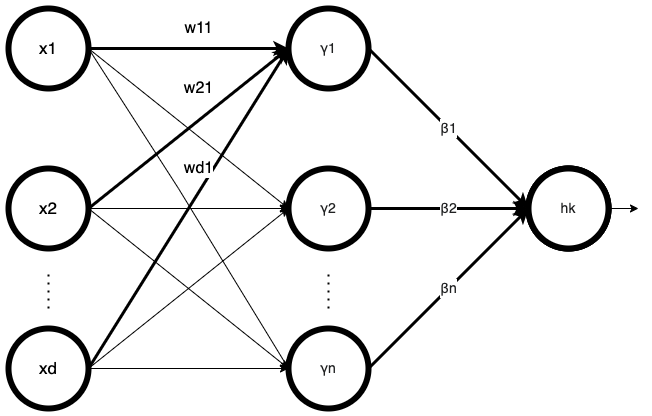
\includegraphics[width=0.85\textwidth]{1-Introduccion_redes_neuronales/Red-Neuronal-una-capa-simple.png}
    \caption{\textit{Grafo} de una red neuronal de una capa oculta}
    \label{img:grafo-red-neuronal-una-capa-oculta_repeticion}
\end{figure}

Ante esta definición el número de parámetros a ajustar es: 
\begin{itemize}
    \item De la forma $\beta_{i k}$: $n s$. 
    \item De la forma $w_{i j}$: $n(d+1)$.
\end{itemize}
Lo que hace un total de $n(s+d+1)$ parámetros, done $n$ es el número de neuronas, $s$ la dimensión de salida y $d$ la dimensión de entrada. Por lo general $d$ y $s$ son fijos a que suponen requisitos del problema, luego si se desea reducir el coste en memoria deberá de hacerse disminuyendo el número de neuronas.

Analizaremos más a fondo su componentes. 

\subsection*{Construcción de la primera capa}
La primera capa está compuesta por el conjunto de $n$ combinaciones
lineales del vector de entrada $(x_1, \ldots, x_d)$
a las cuales denominaremos \textit{activaciones}, $M$ coincide además
con el número de neuronas en la capa oculta. 

\begin{equation}
    a_i = w_{0 i} + \sum_{i=j}^d w_{j i} x_j 
    \text{ con } j \in \{1, \ldots, n \}.
\end{equation}

Nos referiremos a los  parámetros $w_{j i}$ como 
\textit{pesos} y al parámetro $w_{0 i}$ como 
\textit{sesgo}.  

La memoria que necesaria será de de $(d+1)n \mathfrak{F}$ 
con el $\mathfrak{F}$ la memoria requerida por un peso. 
El coste computacional es además de $d$ multiplicaciones 
y $d+1$ sumas.

\subsection*{Unidades ocultas}
Cada una de esas \textit{activaciones} será transformada
utilizando una \textit{función de activación} $\sigma_j$ 

\begin{equation}
    z_i = \gamma_i(a_i).
\end{equation}
En el contexto de las redes neuronales a $z_i$ se le conoce como \textit{unidad oculta}. Ésta  podría ser de 
nuevo  transformada por una combinación lineal, en nuestro caso tan solo 
por el producto de un escalar, ya que como se adelantó en la sección \ref{subsection:diferencia-otras-definiciones-RRNN},
 frente a la transformación afín usualmente propuesta, esta transformación no es necesaria para asegurar la convergencia, profundizaremos más sobre esto más adelante. 

Finalmente la salida vendrá dada por
 \begin{equation}
    h_k = \sum_{i=1}^n \beta_i z_i 
    \text{ con } i \in \{1, \ldots, s \}.
\end{equation}
Nótese que ahora el tamaño de variables de entrada es $M$
y hay un total de $s$ unidades de activación, tanto $M$ como $s$ son
valores fijados por el diseñador de la red ya que a priori no tenemos otra información. 
 
 % Vamos a probar que tampoco mejora el error 
\subsection{Consideraciones sobre la irrelevancia del sesgo}

 Dados $X \subseteq \R^d, Y \subseteq \R^s$ y  $\Gamma$ un conjunto no vacío de funciones medibles definidas de $\R$ a $\R$, denotaremos como $\mathcal{H}^+(X,Y)$ al conjunto de redes neuronales a las cuales se le ha añadido un sesgo. 

\begin{align}
    \mathcal{H}^+(X,Y) 
    =
    \{
        h : X \longrightarrow Y 
        /& \quad 
        h_k(x) = 
        \sum_{i=1}^{n} \left( \beta_{i k} \gamma_{i}( A_{i}(x)) + \alpha_{i k} \right), \\
        & \text{donde  $h_k$  es la proyección k-ésima de $h$ con 
        $k \in \{1, \ldots, s\}$}, \\
        & n \in \N,\gamma_{i} \in \Gamma , \beta_{i k} \in \R
         \text{ y }A_{i} \text{ una aplicación afín de $\R^d$ a $\R$}           
    \}.
\end{align}


Está claro que al introducir tal sesgo se añade en memoria 
un coste de $n \mathfrak{F}$ con $n$ el número de neuronas en la capa oculta y que además el costo de cómputo se ve aumentado en la misma proporción. 

Sin embargo podría obtenerse un beneficio en cuanto a precisión, 
vamos a proceder  a analizar esta idea. 

Es evidente que 
\begin{equation} \label{eq:conjuntos-redes-neuronales-con-sesgo-contiene-elemental}
    \mathcal{H}(X,Y) \subseteq \mathcal{H}^+(X,Y)
\end{equation}

Además al estar trabajando con una sola capa, se tiene que para cualquier 
$h^+ \in \mathcal{H}^+(X,Y)$

\begin{align}
    h^+ = \sum_{i=1}^{n} \left(\beta_{i k} \gamma_{i}( A_{i}(x)) + \alpha_{i k} \right)
    = \sum_{i=1}^{n} \left(\beta_{i k} \gamma_{i}( A_{i}(x))\right) + k 
\end{align}
Con $k \in \R$ un parámetro libre.

Ante esto, al igual que se hacía en el lema \ref{lema:A_3_función_activación_continua_con_arbitaria}
es fácil obtener una neurona de valor constante y por tanto, para un conjunto fijo de neuronas $n$, se tiene que 
\begin{equation}
    \mathcal{H}^+_n(X,Y) \subsetneq  \mathcal{H}_{n+1}(X,Y),
\end{equation}
de esta relación se obtienen dos cosas: 
puesto que $n$ era arbitrario y 
\begin{equation}
    \mathcal{H}(X,Y) = \bigcup_{n \in \N} \mathcal{H}_n (X,Y)
\end{equation}
entonces como espacios de funciones 
\begin{equation}
    \mathcal{H}(X,Y) = \mathcal{H}^+ (X,Y).
\end{equation}
Por otra parte no hace reparar que la precisión que pueda aportar el sesgo es
superada añadiendo una neurona más a un modelo sin sesgo, es más, también se obtiene una mejora en memoria, ya que 
$\mathcal{H}^+_n(X,Y)$ requiere de $n \mathfrak{F}$ espacio de memoria adicional con respecto a $\mathcal{H}_n(X,Y)$
mientras que $\mathcal{H}_{n+1}(X,Y)$ de $(D +1) \mathfrak{F}$
y por lo visto en el teorema de convergencia universal \ref{teo:MFNAUA}, la precisión se consigue añadiendo neuronas (la dimensión de los datos es fija),
luego podemos suponer que $n$ será mayor que $D+1$. 

Hasta ahora hemos comparado la capacidad de expresión 
por la forma de los elementos de los conjuntos, para comparar su bondad aproximando, vamos a fijar  un 
 número de capas ocultas $n$ y 
 y una función de error cualquiera que mida el error dentro 
 del conjunto de entrenamiento
 $E_{\mathcal{D}}:\mathcal{H}^+(X,Y) \longrightarrow \R^+_0$.
 
 Todas las normas en $\R^n$ son equivalentes luego no hay pérdida de generalidad fijando una cualquiera.  

 Definimos también el error dentro del espacio $\Lambda$ como 
 \begin{equation}
    \mathcal{E}_{\mathcal{D}} (\Lambda)
    = \inf \{ E_{\mathcal{D}}(h) : h \in \Lambda\}.
 \end{equation}

Está claro por la relación  
 (\refeq{eq:conjuntos-redes-neuronales-con-sesgo-contiene-elemental})
 que 
 \begin{equation}
    \mathcal{E}_{\mathcal{D}}(\mathcal{H}^+(X,Y))
    \leq
    \mathcal{E}_{\mathcal{D}}(\mathcal{H}(X,Y))
 \end{equation}

 La clave ahora reside en si se satisface la desigualdad opuesta
Es decir, dada cualquier $h^+ \in \mathcal{H}^+_n(X,Y)$ con un error de $E_D(h^+)$ existe $h \in \mathcal{H}_n(X,Y)$  tal que $E_D(h) \leq E_D(h^+).$  
Esto no es posible para todo los casos, fijamos $h^+ \in \mathcal{H}^+_n(X,Y)$ y tomamos como conjunto de datos $\mathcal{D}$ el grafo de $h^+$, es evidente que $E_{\mathcal{D}}(h^+) = 0$ entonces si existiera $h \in \mathcal{H}_n(X,Y)$ con $E_{\mathcal{D}}(h) \leq E_{\mathcal{D}}(h^+)$ necesariamente $E_{\mathcal{D}}(h) = 0$ y entonces $h^+ \in \mathcal{H}_n(X,Y)$ por lo que se tendría que 
$$\mathcal{H}_n(X,Y) = \mathcal{H}_n^+(X,Y)$$ 
lo cual es una contradicción.

Notemos que en la práctica el conjunto $\mathcal{D}$ es finito, 
por lo que habrá situaciones en que para ese conjunto de datos sí  se tenga la misma precisión. 

% Fin de la demostración 

 Concluimos tras todo esto que aunque la precisión que se pueda obtener con funciones de $\mathcal{H}_n(X,Y)$ y $\mathcal{H}^+_n(X,Y)$ es diferente para un mismo número de neuronas $n$, añadiendo una más el sesgo es irrelevante  y además $\mathcal{H}^+_n(X,Y)$ tiene mayor coste computacional, por lo que afirmamos que 
que es un artificio de las redes neuronales multicapa para enlazar una capa con otra y que en redes neuronales de una capa oculta carece de sentido.

% Consideración sobre componer la red neuronal con una función
\subsection{Consideraciones sobre la composición de redes neuronales con otras funciones}

Es usual en la literatura presentar las redes neuronales con la salida compuesta con una función $\theta$, de tal manera que una red neuronal sea de la forma

\begin{equation}
    h_k(x) = \theta_k 
    \left(
        \sum_{i=1}^{n} \beta_{i k} \gamma_{i}
    \left(
        w_{0 i} + \sum_{j=1}^d w_{j i } x_i
    \right) 
    \right)
    \text{ para cada  } k \in \{1, \ldots, s \}.
\end{equation}
El teorema universal de convergencia \ref{teo:MFNAUA} nos asegura 
que dado un número lo suficientemente grande de neuronas tal 
composición no es necesaria, sin embargo a nivel práctico ese 
número de neuronas puede no alcanzarse y por cómo se produce la convergencia el resultado serán funciones con imágenes contenidas en $\R^n$.

Por la naturaleza de la imagen de ciertos problemas no sería necesaria mayor modificación y con nuestra definición sería más que suficiente, pero en caso de la salida tener que cumplir alguna restricción como  un problema de clasificación que necesite una salida discreta por lo observado en \ref{corolario:2_5_función_Booleana} aunque la convergencia esté asegurada para asegurarnos que se cumplen tales restricciones sería necesario la composición con una función $\theta$.

\textcolor{red}{Pensar en el debate de si entrenar y luego determinar $\theta$ o directamente entrenar con $\theta$ (esto vendrá determinado por el método de aprendizaje que usemos y si $\theta$ se lleva bien con él.)}

%%%%%%%%%%% Fin de lo observado

\subsection{Qué función de activación seleccionar}

Los aspectos a tener en cuenta a la hora de seleccionar una función 
de activación frente a otra de una red neuronal serían los siguientes:
\begin{enumerate}
    \item Espacio de memoria.
    \item Coste computacional.
    \item Precisión a obtener.
\end{enumerate}

Sobre la primera consideración está claro que el uso de una única función ahorraría el tener que almacenar el tipo de función que se va emplear en cada neurona.

Respecto al coste computacional para se han observado los siguientes
\textcolor{red}{TODO:  añadir coste computacional  de las funciones que considere oportunas}

Y respecto a la precisión no se conoce ninguna motivación (por ahora)
que \textcolor{red}{TODO pensar}

\textcolor{red}{TODO: Pudiera existir un equilibrio entre 
el coste y la precisión. Es decir, a mismo número de neuronas se podría conseguir mejor precisión con ciertas funciones de activación -> esto seguro. ¿Cómo se podría saber esto a partir de los datos? ¿aumentaría ese proceso el coste?}


%% Formulación técnica 

\section{Explicitación de la construcción y evaluación de una red neuronal}

Ante todas las consideraciones expuestas y puesto que 
no existe ningún resultado o hipótesis a favor de combinar funciones de activación, en pos de simplificar el estudio; vamos a suponer a priori que todos los nodos están compuestos con la misma. Entonces,  una red neuronal para nosotros 
no serán más que dos matrices de pesos y una función de evaluación. 

Es decir siguiendo la idea constructiva expuesta en manuales tales como \cite{learning-from-data-1-2}
 cualquier $h \in \rrnnsmn$ de $n$ neuronas en la capa oculta se implementa como 
$(\gamma, M_{n \times (1+r)}, M_{(n+1) \times s})$ con $M_{f \times c}$ matrices de dimensiones $f$ filas y $c$ columnas. 

$\gamma$ representa a función de activación en cada nodo. 
$M_{n \times (1+r)}$ son los pesos de la primera capa 
y $M_{(n+1) \times s}$ son los pesos de la salida. 

Tomando como $\mathfrak{I}_{r+1}: \R^r \longrightarrow M_{(r+1) \times 1}(\R)$ a la aplicación inyección que a cada vector $(x_1, \ldots, x_d)$ le hace corresponder el vector columna $(1, x_1, \ldots x_d)^T.$
Además entendemos para una función $\gamma : \R \longrightarrow \R$ 
que la imagen de una matriz con $\gamma$ es evaluar cada una de sus entradas por $\gamma$. 
Con esta representación evaluar una red neuronal consistiría en el producto matricial de 

\begin{equation}
    h(x) =  M_{(n+1) \times s} \cdot
    \mathfrak{I}_{n+1}\left(
         \gamma \left( 
             M_{n \times (1+d)} 
            \cdot 
            \mathfrak{I}_{d+1}(x)
        \right)
    \right).
\end{equation}

El coste computacional de tal operación es 
\begin{table}[h]
    \begin{center}
    \begin{tabular}{| c | c |}
    \hline
    Operación & Apariciones  \\ \hline
    $+$ & $n d+n s = n(d+s)$  \\
    $\times$ & $n(d+1)+(n+1)s = n(d+s+2)$  \\
    $\gamma$ & $n$  \\
    $\mathfrak{I}$ & $2$  \\
    \hline
    \end{tabular}
    \caption{Coste computacional de la implementación propuesta en \cite{MostafaLearningFromData}}
    \label{tab:coste computacional de la implementación de Mustafa}
    \end{center}
\end{table}

\subsection*{Primera optimización reformulando la implementación de una red neuronal}

Sin embargo de acorde a nuestro modelo definido en \ref{definition:redes_neuronales_una_capa_oculta}, nuestra propuesta de representación es al siguiente: 

\begin{equation}
    (\gamma, A, S, B) 
    \text{ donde } 
    A \in M_{n \times d}(\R), 
    S\in M_{n \times 1}(\R) 
    \text{ y }
    B \in M_{s \times n}(\R).
\end{equation}
y con esta representación la evaluación sería

\begin{equation}
    h(x) =  B \cdot
        \gamma \left( 
            A
            \cdot 
            x
            + S
        \right),
\end{equation}
que tiene un coste computacional de 
\begin{table}[h]
    \begin{center}
    \begin{tabular}{| c | c |}
    \hline
    Operación & Apariciones  \\ \hline
    $+$ & $n d+n(s-1) = n(d+s-1)$  \\
    $\times$ & $n d+n s = n(d+s)$  \\
    $\gamma$ & $n$  \\
    $\mathfrak{I}$ & $0$  \\
    \hline
    \end{tabular}
    \caption{Coste computacional de nuestra implementación de red neuronal de una capa}
    \label{tab:coste computacional nuestr modelo red neuronal}
    \end{center}
\end{table}

Que como vemos ha supuesto una mejora de 

\begin{table}[h]
    \begin{center}
    \begin{tabular}{| c | c | c | c |}
    \hline
    % cabecera 
    Operación 
    & Coste formulación usual \ref{tab:coste computacional de la implementación de Mustafa}
    & Coste nuestra propuesta \ref{tab:coste computacional nuestr modelo red neuronal} 
    & Operaciones reducidas  \\ \hline
    $+$ & $n(d+s)$ & $n(d+s-1)$ & $n$\\
    $\times$ & $n(d+s+2)$ & $n(d+s)$  & $2n$\\
    $\gamma$ & $n$  & $n$  & $0$ \\
    $\mathfrak{I}$  & $2$ & $0$ & $2$ \\
    \hline
    \end{tabular}
    \caption{Comparativas de coste computacional entre la implementación usual de una red neuronal y la nuestra}
    \label{tab:comparativas coste red neuronal }
    \end{center}
\end{table}

Además se ha reducido el espacio de memoria en $n$ unidades del tipo de datos que utilicen las redes neuronales. 

\subsubsection*{Ejemplo de evaluación de una red neuronal}

\begin{figure}[h!]
    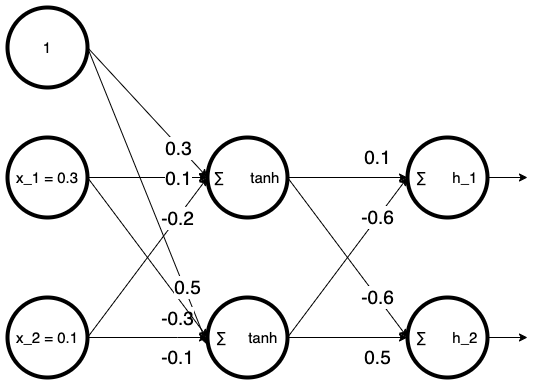
\includegraphics[width=0.7\textwidth]{4-Actualizacion_redes_neuronales/evaluacion-1-capa.drawio.png}
    \centering
    \caption{Ejemplo de evaluación de una red neuronal de una capa con entrada y salida de tamaño dos y dos neuronas en la capa oculta}
    \label{img:Ejemplo-evaluación-red-neruonal-una-capa}
\end{figure}

A continuación vamos a dar un ejemplo basado en la red neuronal mostrada en la imagen \ref{img:Ejemplo-evaluación-red-neruonal-una-capa}, 
La red neuronal viene dada por las matrices: 
la matriz de la primera capa asociada es 
\begin{equation}
     A = 
        \begin{bmatrix}
            0.1 & -0.2 \\
            -0.3 & -0.1 
        \end{bmatrix}  
\end{equation}
la matriz de sesgos 
\begin{equation}
    S = 
        \begin{bmatrix}
            0.3  \\
            0.5 
        \end{bmatrix}  
\end{equation}
La matriz de pesos de la capa oculta sería 
\begin{equation}
     B = 
    \begin{bmatrix}
        0.1 & -0.6 \\
        -0.6 & 0.5
    \end{bmatrix}. 
\end{equation}

Para la entrada  $x = (0.3, 0.1)$ los sucesivos cálculos serían
\begin{equation}
    A x = 
    \begin{bmatrix}
        0.1 & -0.2 \\
        -0.3 & -0.1 
    \end{bmatrix}  
    \begin{bmatrix}
        0.3  \\
        0.1 
    \end{bmatrix}
    = 
    \begin{bmatrix}
        0.01  \\
        -0.1 
    \end{bmatrix}
    . 
\end{equation}

\begin{equation}
    A x +S= 
    \begin{bmatrix}
        0.01  \\
        -0.1 
    \end{bmatrix}
    + 
    \begin{bmatrix}
        0.3  \\
        0.5 
    \end{bmatrix}
    = 
    \begin{bmatrix}
        0.31  \\
        0.4 
    \end{bmatrix}
    . 
\end{equation}

\begin{equation}
    \gamma (A x +S) = 
    \gamma \left(
    \begin{bmatrix}
        0.31  \\
        0.4 
    \end{bmatrix}
    \right)
    = 
    \begin{bmatrix}
        \gamma(0.31)  \\
        \gamma(0.4) 
    \end{bmatrix}
    = 
    \begin{bmatrix}
        0.3004 \\
        0.3799  \\
    \end{bmatrix}.
\end{equation}

Finalmente las respectivas salidas de las capas ocultas serían
\begin{equation}
    B  \gamma (A x +S)  
    = 
    \begin{bmatrix}
        0.1 & -0.6 \\
        -0.6 & 0.5
    \end{bmatrix}
    \begin{bmatrix}
        0.3004 \\
        0.3799  \\
    \end{bmatrix}
    = 
    \begin{bmatrix}
        -0.1979 \\
       0.0097  \\
    \end{bmatrix}.
\end{equation}

\subsection{Implementación de una red neuronal y evaluación}

Como conclusión a todo lo explicado una red neuronal no sería más que una estructura que almacenara $(\gamma, A, S, B)$, esto es 

% Pseudo código que refleja la estructura de una red neuronal 

\begin{algorithm}[H]
    \caption{Estructura de una red neuronal}
    \label{algoritmo:estructura de una red neuronal}
    \DontPrintSemicolon
    \hspace*{\algorithmicindent} 
        \textbf{Entrada}:
        \begin{itemize}
            \item $d$: Dimensión de los datos de entrada.
            \item $s$: Dimensión que define una red neuronal.
            \item $n$: Número de redes nodos en la capa oculta. 

        \end{itemize}
        \hspace{\algorithmicindent} 
        \Struct{Red neuronal(d,s,n)}{
            $A \gets$ Matriz $n$ filas $d$ columnas\;
            $S \gets$ Matriz $n$ filas $1$ columnas\;
            $B \gets$ Matriz $s$ filas $n$ columnas\;
        }
        \hspace{\algorithmicindent} 
  \end{algorithm}

y si quisiéramos evaluar la red neuronal el algoritmo sería el siguiente 
  %% Algoritmo de evaluación de redes neuronales 

  \begin{algorithm}[H]
    \caption{Evaluación de una red neuronal, \textit{Forward propagation}}
    \label{algoritmo:evaluar red neuronal}

    \hspace*{\algorithmicindent} 
        \textbf{Entrada}:
        \begin{itemize}
            \item $x$: Vector de atributos que se desea evaluar con la red neuronal.
            \item $h = (\gamma, A, S, B)$ representa la red neuronal que se desea evaluar y la función de activación $\gamma$ con la que se va a evaluar. 
        \end{itemize}
        \hspace{\algorithmicindent} 
        \SetKwFunction{Main}{ForwardPropagation}
        \SetKwProg{F}{Function}{:}{}
        \F{\Main{$h, x$}}{ 

            sensibilidad $\gets A \cdot x + S$ \;
            primeraCapa $\gets$ sensibilidad \;
            \ForEach{ entrada-Iésima-Neurona $\in$ sensibilidad}{
                primeraCapa[i] $\gets \gamma($ entrada-Iésima-Neurona $)$
            }
            \;
            salida $\gets B \cdot $primeraCapa \;
            \KwRet salida \;
        }
  \end{algorithm}
  \newpage







\section{Aprendizaje}  

Se entiende por aprendizaje de una red neuronal como el proceso 
por el cual se determina el valor sus pesos, es decir, lo que en el ejemplo \ref{img:Ejemplo-evaluación-red-neruonal-una-capa} consistía en las matrices $A,S$ y $B$.

%%%%%%%%%%%%%%%%%%% algoritmo de gradiente descendente 

\subsection{Método de gradiente descendente y \textit{backpropagation}} \label{sec:gradiente-descendente}

De acorde a los capítulos uno y dos del libro  \cite{learning-from-data-1-2},
 una vez concretado el problema y sus elementos 
(\ref{sub:componentes_aprendizaje}) es necesario definir un método con 
el que aproximar la función ideal $f,$ para ello introduciremos el algoritmo de gradiente descendente.  

El gradiente descendente es un método iterativo de minimización de funciones diferenciables. 

% Nota sobre el algoritmo de gradiente descendente 
\reversemarginpar
\marginpar{
    \textcolor{dark_green}{    
        \textbf{
            Aclaración gradiente red neuronal
        }
    }

    Puede a priori uno confundirse con la notación,  
    pero recordemos que las redes neuronales estaban determinadas por sus parámetros (matrices), luego lo único que se está haciendo es derivar con respecto a tales parámetros.
} 
%Fin nota margen
% Idea  sobre el algoritmo de gradiente descendente 
\marginpar{
    \textcolor{dark_green}{    
        \textbf{
            Idea general del algoritmo gradiente descendente
        }
    }

    Cada iteración se obtendrá una nueva red neuronal con un error menor dentro de los datos de entrenamiento del conjunto.
} 

% Nota margen sobre diferenciabilidad
\normalmarginpar
\setlength{\marginparwidth}{\smallMarginSize}
\marginpar{
    \textcolor{red}{    
        \textbf{
            Consecuencia del requisito de diferenciabilidad 
            de $E(h)$
        }
    }
    $E(h)$ será diferenciable si y sólo si las funciones de activación lo son. 
}


%Fin nota margen
En nuestro caso particular se quiere aproximar la función ideal desconocida $f$ a partir de funciones (redes neuronales) $h \in \rrnnmc$, concretamente se fijará un número $n$ de neuronas en la capa oculta. 
Dada también una función de error diferenciable y que no presente puntos de inflexión
$E: \rrnnsmn\longrightarrow \R,$
se toma red neuronal cualquiera $h_0 \in \rrnnsmn$ y 
fijado $\eta \in \R^+$. 

Se define la sucesión 
\begin{equation}\label{eq:descenso-gradiente}
    h_{t+1}  = h_t - \eta \nabla E(h_t).
\end{equation}  

Donde $h_n$ es una sucesión cuyos términos convergen a un mínimo local.
\subsubsection*{Observaciones sobre el algoritmo }

\begin{itemize}
    \item El algoritmo solo encuentra óptimos locales con una dependencia crucial del valor de inicio. 
    \item La convergencia no es segura en un tiempo finito y requiere de criterios de parada. 
    \item Debe de fijarse el número de neuronas en la capa oculta a priori.
    \item Si la función es convexa el mínimo será global.
    \item El parámetro $\eta$ puede ser cualquiera y debe de ser fijado o controlado por el diseñador.  
\end{itemize}


Con el fin de reducir el coste del cálculo del gradiente, 
se utiliza generalmente el algoritmo conocido como \textit{backpropagation} que fue publicado en 
1989 en el artículo \cite{backpropagation-Hinton}. Las hipótesis bajo las que fue diseñado tal algoritmo fueron: redes neuronales con varias capas y entendiendo por red neuronal un modelo más costoso al nuestro. \textbf{Es por ello que a continuación plantearemos una versión propia deducida y optimizada de acorde a nuestro modelo}

 Sea $E_{in} : \rrnnmc \longrightarrow \R^+_0$ la función para medir error habitualmente usada, la cual tomaremos como el error dentro de conjunto de entrenamiento, esto es,  si el conjunto 
de entrenamiento $\mathcal{D}$ está constituido por $N$ datos de la forma $(x_i, y_i)$ con $x_i$ el vector de entrada o atributos y $y_i$ el estado o valor deseado para cualquier $k\in \{1, \ldots, N\}.$ Para cualquier $h \in \rrnnmc$ denotando por $h_k$ a su $k-$ésima proyección, se define como métrica de error dentro de $\mathcal{D}$ como
\begin{equation}
    E_{in}(h) = \frac{1}{N} \sum_{(x,y) \in \mathcal{D}} \sum_{k=1}^s(h_k(x)- y_k)^2. 
\end{equation}

puesto que $\frac{1}{N}$ no es más que una constante de proporcionalidad (y que por tanto no afecta a la minimización) del error y que además 
puede ser corregida en \refeq{eq:descenso-gradiente} con $\eta$, con el fin de ahorrar coste computacional la 
fijaremos a conveniencia. Es decir, podemos suponer que 
nuestra función de error a minimizar es 

\begin{equation}
    E_{in}(h) = \frac{1}{2} \sum_{(x,y) \in \mathcal{D}} \sum_{k=1}^s (h_k(x)- y_k)^2. 
\end{equation}

Antes de adentrarnos en los cálculos tengamos presente que hemos definido una red neuronal  $h \in \mathcal{H}_n (\R^d, \R^s)$ como $h= (h_1, \ldots, h_s)$ con cada proyección $k-$ésima dada por: 
\begin{equation}\label{eq:red-neuronal-que-aprender}
    h_k(x) = 
    \sum_{j=1}^n \beta_{j k}
    \sigma
    \left(  
        \alpha_{0 j} +
        \sum_{i=1}^d \alpha_{i j}x_i
    \right)
\end{equation}
para la cual hemos impuesto que la función de activación $\sigma$ sea diferenciable.

Denotaremos como $\chi_{[c]}$ a la función características
\begin{equation}
    \chi_{[c]}= \left\{ \begin{array}{lcc}
        1 &   si  &  \text{se satisface c} \\
        \\ 0 &  si  & \text{no se satisface c} 
        \end{array}
\right.
\end{equation}

Así pues, en base al modelo expuesto en \refeq{eq:red-neuronal-que-aprender} a la hora de calcular el gradiente del error con respecto a los parámetros que determinan la red, tendríamos tres tipos de derivadas parciales, las dependientes de $\beta_{j  k}$, 
las de $\alpha_{0 j}$ y las de $\alpha_{j i}$, para cada caso concreto y en virtud de la regla de la cadena, se tiene: 

\begin{itemize}
    \item Derivada parcial del error con respecto a $\beta_{v w}$ donde $v \in \{1, \ldots, n\}$ y $w \in \{1, \ldots, s\}$:
    \begin{align} \label{eq:parcial_beta}
        \frac{\partial E(h)}{\partial \beta_{v w}} 
        = &
        \frac{\partial}{\partial \beta_{v w}}
        \left[
            \frac{1}{2}
            \sum_{(x,y) \in \mathcal{D}}
            \sum_{k = 1}^s 
            \left(h_k(x) - y_k \right)^2
        \right]
        \\ % primer paso regla de la cadena
        = &
        \frac{1}{2}
        \sum_{(x,y) \in \mathcal{D}}
        \sum_{k = 1}^s 
        2 \left(h_k(x) - y_k \right)
        \frac{\partial h_k(x)}{\partial \beta_{v w}} 
        \\ 
        = & % desarrollamos h
        \sum_{(x,y) \in \mathcal{D}}
        \sum_{k = 1}^s 
        \left(h_k(x) - y_k \right)
        \frac{\partial}{\partial \beta_{v w}} 
        \left[
            \sum_{j = 1}^n 
                \beta_{j k}
                \sigma
                \left(  
                    \alpha_{0 j} +
                    \sum_{i=1}^d \alpha_{i j}x_i
                \right)
        \right] 
        \\ 
        = & % parcial de la suma es suma de parciales 
        \sum_{(x,y) \in \mathcal{D}}
        \sum_{k = 1}^s 
        \left(h_k(x) - y_k \right)
        \left(
            \sum_{j = 1}^n 
            \frac{\partial}{\partial \beta_{v w}} 
            \left[
                \beta_{j k}
                \sigma
                \left(  
                    \alpha_{0 j} +
                    \sum_{i=1}^d \alpha_{i j}x_i
                \right)
            \right]
        \right) 
        \\ 
        = & % Expresión a partir de la función caraterísticas
        \sum_{(x,y) \in \mathcal{D}}
        \sum_{k = 1}^s 
        \left(h_k(x) - y_k \right)
        \left(
            \sum_{j = 1}^n 
                \chi_{[j = v \wedge k = w]}
                \sigma
                \left(  
                    \alpha_{0 j} +
                    \sum_{j=1}^d \alpha_{i j}x_i
                \right)
        \right)
        \\ 
        = & % Expresión final quitando términos nulos 
        \sum_{(x,y) \in \mathcal{D}}
        \left(h_w(x) - y_w \right)
        \left(
            \sigma
            \left(  
                \alpha_{0 v} +
                \sum_{i=1}^d \alpha_{i v}x_i
            \right)
        \right).
    \end{align}

    \item Derivada parcial del error con respecto a $\alpha_{0 v}$ donde $v \in \{1, \ldots, n\}$:
    \begin{align} \label{eq:parcial_alpha_cero}
        \frac{\partial E(h)}{\partial \alpha_{0 v}} 
        = &
        \frac{\partial}{\partial \alpha_{0 v}}
        \left[
            \frac{1}{2}
            \sum_{(x,y) \in \mathcal{D}}
            \sum_{k = 1}^s 
            \left(h_k(x) - y\right)^2
        \right]
        \\ % primer paso regla de la cadena
        = &
        \frac{1}{2}
        \sum_{(x,y) \in \mathcal{D}}
        \sum_{k = 1}^s 
        2 \left(h_k(x) - y_k \right)
        \frac{\partial h_k(x)}{\partial \alpha_{0 v}} 
        \\ 
        = & % desarrollamos h
        \sum_{(x,y) \in \mathcal{D}}
        \sum_{k = 1}^s 
        \left(h_k(x) - y_k \right)
        \frac{\partial}{\partial \alpha_{0 v}} 
        \left[
            \sum_{j = 1}^n 
                \beta_{j k}
                \sigma
                \left(  
                    \alpha_{0 j} +
                    \sum_{i=1}^d \alpha_{i j}x_i
                \right)
        \right] 
        \\ 
        = & % parcial de la suma es suma de parciales 
        \sum_{(x,y) \in \mathcal{D}}
        \sum_{k = 1}^s 
        \left(h_k(x) - y_k \right)
        \left(
            \sum_{j = 1}^n 
            \beta_{j k}
            \frac{\partial}{\partial \alpha_{0 v}} 
            \left[
                \sigma
                \left(  
                    \alpha_{0 j} +
                    \sum_{i=1}^d \alpha_{i j}x_i
                \right)
            \right]
        \right) 
        \\ 
        = & %regla de la cadena 
        \sum_{(x,y) \in \mathcal{D}}
        \sum_{k = 1}^s 
        \left(h_k(x) - y_k \right)
        \left(
            \sum_{j = 1}^n 
            \beta_{j k}
            \sigma '
            \left(  
                \alpha_{0 j} +
                \sum_{i=1}^d \alpha_{i j}x_i
            \right)
            \frac{\partial}{\partial \alpha_{0 v}}    
            \left[
                \alpha_{0 j} +
                \sum_{i=1}^d \alpha_{i j}x_i
            \right]
        \right) 
        \\ 
        = & % función característica
        \sum_{(x,y) \in \mathcal{D}}
        \sum_{k = 1}^s 
        \left(h_k(x) - y_k \right)
        \left(
            \sum_{j = 1}^n 
            \beta_{j k}
            \sigma '
            \left(  
                \alpha_{0 j} +
                \sum_{i=1}^d \alpha_{i j}x_i
            \right)   
            \chi_{[j = v]}
        \right) 
        \\ 
        = & % Expresión final quitando términos nulos 
        \sum_{(x,y) \in \mathcal{D}}
        \sum_{k = 1}^s 
        \left(h_k(x) - y_k \right)
        \left(
            \beta_{v k}
            \sigma '
            \left(  
                \alpha_{0 v} +
                \sum_{i=1}^d \alpha_{i v}x_i
            \right)   
        \right). 
    \end{align}

    \item Derivada parcial del error con respecto a $\alpha_{u v}$ donde $u \in \{1, \ldots, d\}$ y $v \in \{1, \ldots, n\}$:
    
    \begin{align} \label{eq:parcial_alpha_i}
        \frac{\partial E(h)}{\partial \alpha_{u v}} 
        =&
        \frac{\partial}{\partial \alpha_{u v}}
        \left[
            \frac{1}{2}
            \sum_{(x,y) \in \mathcal{D}}
            \sum_{k = 1}^s 
            \left(h_k(x) - y_k \right)^2
        \right]
        \\ % primer paso regla de la cadena
        = &
        \frac{1}{2}
        \sum_{(x,y) \in \mathcal{D}}
        \sum_{k = 1}^s 
        2 \left(h_k(x) - y_k \right)
        \frac{\partial h_k(x)}{\partial \alpha_{u v}} 
        \\ 
        = & % desarrollamos h
        \sum_{(x,y) \in \mathcal{D}}
        \sum_{k = 1}^s 
        \left(h_k(x) - y_k \right)
        \frac{\partial}{\partial \alpha_{u v}} 
        \left[
            \sum_{j = 1}^n 
                \beta_{j k}
                \sigma
                \left(  
                    \alpha_{0 j} +
                    \sum_{i=1}^d \alpha_{i j}x_i
                \right)
        \right] 
        \\ 
        = & % parcial de la suma es suma de parciales 
        \sum_{(x,y) \in \mathcal{D}}
        \sum_{k = 1}^s 
        \left(h_k(x) - y_k \right)
        \left(
            \sum_{j = 1}^n 
            \beta_{j k}
            \frac{\partial}{\partial \alpha_{u v}} 
            \left[
                \sigma
                \left(  
                    \alpha_{0 j} +
                    \sum_{i=1}^d \alpha_{i j}x_i
                \right)
            \right]
        \right) 
        \\ 
        = & %regla de la cadena 
        \sum_{(x,y) \in \mathcal{D}}
        \sum_{k = 1}^s 
        \left(h_k(x) - y_k \right)
        \left(
            \sum_{j = 1}^n 
            \beta_{j k}
            \sigma '
            \left(  
                \alpha_{0 j} +
                \sum_{i=1}^d \alpha_{i j}x_i
            \right)
            \frac{\partial}{\partial \alpha_{u v}}    
            \left[
                \alpha_{0 j} +
                \sum_{i=1}^d \alpha_{i j}x_i
            \right]
        \right) 
        \\ 
        = & % función característica
        \sum_{(x,y) \in \mathcal{D}}
        \sum_{k = 1}^s 
        \left(h_k(x) - y_k \right)
        \left(
            \sum_{j = 1}^n 
            \beta_{j k}
            \sigma '
            \left(  
                \alpha_{0 j} +
                \sum_{i=1}^d \alpha_{i j}x_i
            \right)   
            \chi_{[i = u\wedge j = v]}x_i
        \right) 
        \\ 
        = & % Expresión final quitando términos nulos 
        \sum_{(x,y) \in \mathcal{D}}
        \sum_{k = 1}^s 
        \left(h_k(x) - y_k \right)
        \left(
            \beta_{v k}
            \sigma '
            \left(  
                \alpha_{0 v} +
                \sum_{i=1}^d \alpha_{i v}x_i
            \right)x_u   
        \right).
    \end{align}
\end{itemize}  

Recapitulando los resultados, el cálculo de las derivadas parciales con $u \in \{1, \ldots, d\}$, $v \in \{1, \ldots, n\}$ y $w \in \{1, \ldots, s\}$ consiste en: 

% Resumen desarrollo anterior: 
\begin{itemize}
    \item Por el desarrollo (\ref{eq:parcial_beta}) la derivada parcial del error con respecto a $\beta_{v w}$ es:
    \begin{align} 
        \frac{\partial E(h)}{\partial \beta_{v w}} 
        = & % Expresión final quitando términos nulos 
        \sum_{(x,y) \in \mathcal{D}}
        \left(h_w(x) - y_w \right)
        \left(
            \sigma
            \left(  
                \alpha_{0 v} +
                \sum_{i=1}^d \alpha_{i v}x_i
            \right)
        \right).
    \end{align}

    \item Por el desarrollo (\ref{eq:parcial_alpha_cero}) derivada parcial del error con respecto a $\alpha_{0 v}$ es :
    \begin{align} 
        \frac{\partial E(h)}{\partial \alpha_{0 v}} 
        =  % Expresión final quitando términos nulos 
        \sum_{(x,y) \in \mathcal{D}}
        \sum_{k = 1}^s 
        \left(h_k(x) - y_k \right)
        \left(
            \beta_{v k}
            \sigma '
            \left(  
                \alpha_{0 v} +
                \sum_{i=1}^d \alpha_{i v}x_i
            \right)   
        \right). 
    \end{align}

    \item Por el desarrollo (\ref{eq:parcial_alpha_i}) derivada parcial del error con respecto a $\alpha_{u v}$:
    \begin{align} 
        \frac{\partial E(h)}{\partial \alpha_{u v}} 
        =
        \sum_{(x,y) \in \mathcal{D}}
        \sum_{k = 1}^s 
        \left(h_k(x) - y_k\right)
        \left(
            \beta_{v k}
            \sigma '
            \left(  
                \alpha_{0 v} +
                \sum_{i=1}^d \alpha_{i v}x_i
            \right)x_u   
        \right).
    \end{align}
\end{itemize}  

% Consideración sobre los costes 
Si el cálculo se hiciera sin tener más consideración alguna que la propia expresión e incluso obviando el coste de aplicar \textit{forward propagation}, la diferencia y el producto
supondría el cómputo que mostramos en la tabla \ref{tab:coste-computacional-directa}.

% tabla con coste en multiplicación 
\begin{table}[H]
    \begin{center}
    \resizebox{\textwidth}{!}{
    \begin{tabular}{| c | c | c | c | c | c| }
    \hline
    % cabecera
       & Número de parámetros & $+ / -$ & $\times / \div$ & $\sigma$ & $\sigma'$
    \\ \hline
    % Para betas
    (\ref{eq:parcial_beta}) $\frac{\partial h(x))}{\partial \beta_{j k}}$ 
    & $n s$ & $n s (d+1)$ & $n s d$ & $n s$ & 0
    \\
    \hline
    % Para los segos alpha 0i 
    (\ref{eq:parcial_alpha_cero}) $\frac{\partial h(x)}{\partial \alpha_{0 i}}$ 
    & $n$ & $n d$ & $n (d + 1)$ & 0 & $n$
    \\
    \hline
    % Para los segos alpha ji 
    (\ref{eq:parcial_alpha_i}) $\frac{\partial h(x)}{\partial \alpha_{i j}}$ 
    & $n d$ & $n d^2$ & $n d (d + 2)$ & 0 & $n d$
    \\
    \hline
    % Para los segos alpha ji 
    \textit{forward propagation}
    & $n (s+1+d)$ & $n^2 (d+s)(s-1+d)$ & $ n^2 (s+1+d)(d + s)$ & n & 0
    \\
    \hline
    \end{tabular}
    }
    \caption{Coste computacional de aplicar directamente el  algoritmo de gradiente 
    descendente para actualizar $h \in \mathcal{H}_n(\R^d, \R^s)$}
    \label{tab:coste-computacional-directa}
    \end{center}
\end{table}

Abordar el problema de manera directa es muy ineficiente. Basta fijar un par $(x,y) \in \mathcal{D}$ para darse cuenta de que el cálculo de $h(x)-y$ se repite $n(s+1+d)$ veces y que además,  como mostramos en la tabla 
\ref{tab:expresiones_repetidas_en_descenso_gradiente}
hay cálculos que se repiten en (\refeq{eq:parcial_beta}), (\refeq{eq:parcial_alpha_cero}) y  
(\refeq{eq:parcial_alpha_i}). 

\begin{table}[H]
    \begin{center}
        \resizebox{\textwidth}{!}{
    \begin{tabular}{| c | c | c | c | c| c | c| }
    \hline
    % cabecera
    Expresión  repetida en 
    & $\frac{\partial E(h)}{\partial \beta_i}$ 
    & $\frac{\partial E(h)}{\partial \alpha_{0 i}}$ 
    &$\frac{\partial E(h)}{\partial \alpha_{j i}}$ 
    & Total apariciones  para $i$
    & Coste total 
    & Coste en memoria 
    \\ \hline
    % Primer cálculo repetido 
    $\alpha_{0 i} \sum_{j=1}^d \alpha_{j i}x_j$ 
    & 1 & 1& $d$ & $d+2$ & $n(d+2)$ & $n$
    \\
    % Segundo cálculo repetido
    $\beta_{i k} \sigma'
    \left(  
     \alpha_{0 i} 
     \sum_{j=1}^d \alpha_{j i}x_j
    \right)$
    & 0 & 1 & $d$ & $d+1$ & $n s(d+1)$ &$n s$
    \\ \hline
    \end{tabular}
        } % fin ajuste tamaño
    \caption{Veces que se calcula una misma expresión 
    para el cálculo de gradiente descendente fijado un
     $i$ y coste en memoria en unidades si se almacenara el cálculo de todos esos parámetros.}
    \label{tab:expresiones_repetidas_en_descenso_gradiente}
    \end{center}
\end{table}

Notemos además que las expresiones del tipo 
$\alpha_{0 j} + \sum_{i=1}^d \alpha_{i j}x_i$  son las que denotábamos como $sensibilidades$ en el algoritmo de \textit{forward propagation} \ref{algoritmo:evaluar red neuronal}.
 

\subsection{ Motivación para almacenar cálculos parciales}  

A la vista de las repeticiones de cálculos, su coste computacional,
 ofrece un gran beneficio almacenar $h_k(x)-y_k$, ya que el coste de cálculo aumenta de manera lineal conforme aumenta el número de neuronas mientras que se mantiene constante el costo en memoria.      

Para el resto de expresiones podría no estar tan claro su beneficio, 
ya que estamos en una situación en la que el coste en memoria y de cálculo aumentan manera lineal con respecto al número de neuronas. 

Sin embargo, para un cálculo directo sin almacenar operaciones intermedias, sería necesario reservar en memoria espacio para $n (s + 1 + d )$  parámetros, ya que no se debería de sobreescribir los parámetros antiguos con los nuevos ya que afectaría al cálculo. 

Pero como hemos observado en el coste en memoria de ir almacenando los resultados parciales \ref{tab:expresiones_repetidas_en_descenso_gradiente} y se aprecia claramente en \ref{algoritmo:calculo-gradiente}
el coste en memoria de nuestro algoritmo sería de $ n (d + 2s +3) +1$.
Así pues se acaba de probar que un algoritmo directo es peor en coste de cálculo y ligeramente memoria frente a otro que almacene los resultados parciales. 

Por lo que los algoritmos que proponemos a continuación se basarán en almacenar estos resultados. 

\subsection{Algoritmos de actualización de pesos de una neurona}

Nuestro objetivo es aplicar el algoritmo de gradiente descendente, codificaremos una red neural $h \in \rrnnsmn$ de estructura $(A,S,B)$, como dos matrices de parámetros $\alpha$ y $\beta$ y de respectivos tamaños $d \times(n+1)$ y $s \times n$: 

\begin{align}\label{eq:representation red neuronal}
    A &= (\alpha_{i,j}) \text{ con }  i \in \{1, \ldots d\}, \; j \in \{1, \ldots n\}. \\
    S &= (\alpha_{0, j}) \text{ con }  j \in \{1, \ldots, n\}. \\
    B &= (\beta_{j,k}) \text{ con }  j \in \{1, \ldots n\}, \; k \in \{1, \ldots s\}.\\
\end{align}
 De esta manera $h$ modificará el valor de sus pesos de acorde al algoritmo de gradiente descendente \ref{eq:descenso-gradiente} que viene dado por

\begin{algorithm}[H]
    \caption{Algoritmo gradiente descendente.}
    \hspace*{\algorithmicindent} \textbf{Input}:$h$ red neuronal  y conjunto de entrenamiento \\
    \hspace*{\algorithmicindent} \textbf{Output:} $h$ actualizada de acorde al algoritmo de gradiente descendente. 
    \begin{algorithmic}[1]
        \STATE Debe de calcularse el previamente el $\nabla E(h)$, es decir cada una de la parciales.
        % actualizamos los pesos de a 
        \STATE Actualización de los pesos de $A$ \\  
        \For{
                $j \in \{1,\ldots n\}$
            }{
                \For{
                $i \in \{1,\ldots d\}$
            }{
                \begin{equation}
                    \alpha_{i j} 
                    \gets 
                    \eta 
                    \frac{\partial E(h)}{\partial \alpha_{i j}}
                \end{equation}
            }
        }
         %  Actualizamos los pesos de S               
        \STATE Actualización de los pesos de $S$ \\   
        \For{
                $j \in \{1,\ldots n\}$
            }{
                \begin{equation}
                    \alpha_{0 j} 
                    \gets 
                    \eta 
                    \frac{\partial E(h)}{\partial \alpha_{0 j} }
                \end{equation}
        } 
        % actualizamos los pesos de B
        \STATE Actualización de los pesos de $B$ \\ 
        \For{
                $k \in \{1,\ldots s\}$
            }{
                \For{
                $j \in \{1,\ldots n\}$
            }{
                \begin{equation}
                    \beta_{j k} 
                    \gets 
                    \eta 
                    \frac{\partial E(h)}{\partial \beta_{j k}}
                \end{equation}
            }
        }
\end{algorithmic}
\end{algorithm}

Notemos la necesidad de una variable $\eta \in \R$ que es prefijada. 

\textcolor{red}{$\eta$ podría ser incluso una vector de pesos que se aplicara de manera distinta a cualquier coeficiente o una función variable de ciertas condiciones. No sé hasta qué punto sería interesante plantearse el uso de algoritmos genéticos para actualizarlo ya que estos carecen de valor teórico. ¿Existe algún resultado de análisis que nos de una cota mejor?}


Procederemos ahora a determinar el cálculo del gradiente, como hemos visto este vienen determinado por la expresión. 

El algoritmo que se muestra a continuación supone que la memoria no es un problema así que se plantea para que el no haya ningún cálculo repetido. 

\textcolor{red}{ Falta revisar que esté bien este algoritmo}

% Cálculo de los gradientes 
\begin{algorithm}[H] \label{algoritmo:calculo-gradiente}
    \caption{Algoritmo cálculo del gradiente $\nabla E(h)$.}
    \hspace*{\algorithmicindent} \textbf{Input}:$h \in  \rrnnsmn$ red neuronal que representaremos como en \ref{eq:representation red neuronal} y $\mathcal{D}$ conjunto de entrenamiento, con pares $(x, y)$. \\
    \hspace*{\algorithmicindent} \textbf{Output:} Gradiente del error, esto es $\nabla E(h)$ que se almacena en las siguientes variables: 
    \begin{itemize}
        \item $\text{parcial} \alpha_{i j}$ hace referencia a $\frac{\partial E(h)}{\partial \alpha_{i j}}$. 
   
        \item $\text{parcial} \beta _{i j}$ hace referencia a $\frac{\partial E(h)}{\partial \beta _{i j}}$. 
    \end{itemize} 
    \begin{algorithmic}[1]
        \STATE Inicializamos respectivamente las variable que contendrán a las derivadas parciales
        \begin{itemize}
            \item $\text{parcial} \alpha_{i j} \gets$ matriz de reales de tamaño $n+1 \times d$ con entradas a cero. 
            \item $\text{parcial} \beta_{i j} \gets$ matriz de reales de tamaño $s \times n$ con entradas a cero. 
        \end{itemize}
        \STATE 
        \For{ cada para $(x,y) \in \mathcal{D}$}{
            \STATE Calculamos \textit{forward propagation }
            \For{ cada $i \in \{1, \ldots n\}$}{
                \STATE Cálculo de las sensibilidades vector $\delta$ donde su componente $i-$ésima viene dada por \\
                $\delta_i \gets \alpha_{0 i} + \sum_{j = 1}^d \alpha_{j i} x_j$.
                \STATE Cálculo de la salida de los nodos, vector $s$ donde cada componente es \\
                $s_i \gets \sigma (\delta_i)$. 
                \STATE Almacenamos las derivadas \\
                $\text{ds}_i \gets \sigma' (\delta_i)$. \\
                \For{cada $k \in \{1, \ldots s\}$}{
                    $\text{derivada} \beta_{i k } \gets
                     \beta_{i k} \text{ds}_i$
                }
            }
            \STATE $h_{x} \gets B s$  (se multiplica la matriz de coeficientes de la red neuronal por la salida previamente calculada)
            \STATE $\text{diferencia} \gets h_{x} - y$  
        
            % Cálculo del  gradiente
            % cálculo de los betas
            \STATE Cálculo de gradiente de $\frac{\partial E(h)}{\partial \beta _{u v}}$\\  
            \For{
                    $u \in \{1,\ldots n\}$
                }{
                    \For{
                    $v \in \{1,\ldots s\}$
                }{
                 
                        $\text{parcial} \beta _{u v} 
                        \gets 
                        \text{parcial} \beta _{u v} 
                        + 
                        \text{diferencia}_v  s_i$.
                    
                }
            }
            % Cálculo de alpha
            \STATE Cálculo del tipo $\frac{\partial E(h)}{\partial \alpha _{u v}}$\\  
            \For{
                    $v \in \{1,\ldots n\}$
                }{
                    \For{
                        $k \in \{1,\ldots s\}$
                    }{
                        
                        $\text{auxiliarDiferenciaPorDerivada}
                            \gets
                                \text{diferencia}_k 
                                \,
                                \text{derivada} \beta_{v k}$. \\
                        
                        $\text{parcial} \alpha _{0 v} 
                            \gets 
                            \text{parcial} \alpha _{0 v} 
                            + 
                            \text{auxiliarDiferenciaPorDerivada}$.
                        

                        \For{
                            $u \in \{1,\ldots d\}$
                        }{
                           
                            $\text{parcial} \alpha _{u v} 
                                \gets 
                                \text{parcial} \alpha _{u v} 
                                + 
                                \text{auxiliarDiferenciaPorDerivada}
                                \, 
                                x_u$.
                            
                        }
                    }
                }
            
        }
\end{algorithmic}
\end{algorithm}

\textcolor{red}{Falta añadir complejidad}

\subsubsection*{Análisis de la complejidad}  
Notemos que la complejidad computacional del algoritmo  \ref{algoritmo:calculo-gradiente} es:
\begin{itemize}
    \item \textbf{Coste de cálculo}:  Entiendo suma, productos y evaluaciones como constante de valor $1$ el resultado es: 
    \begin{align}
        \text{coste} &=
        |\mathcal{D}| 
        \left(
            n(1+1+1 + s) + 
            1+1 +
            n s 
            + n s (1 + 1 + d) 
        \right) 
        \\
        & =   
        |\mathcal{D}| 
        ( 
            n (3 + s)  
            +  3 n s
            + n s d
        ) 
        \\
        & = |\mathcal{D}|
        (
            4 n s + d n s + 3 n
        )  
        \\
        & \leq 
        |\mathcal{D}|
        3 \max \{4, d \} n s.
    \end{align} 

    De aquí se deduce, puesto que $s,d$ son constantes fijas que a nivel práctico serán mucho menor que el número de neuronas  $n$ y el número de datos de entrenamiento $|\mathcal{D}| $, que los que afecta primordialmente al coste es $|\mathcal{D}| $ y $n$. 
    
    Si queremos converger con cierta precisión, el teorema de aproximación no nos permite reducir $n$. Sin embargo, si suponemos que $\mathcal{D}$
    presenta datos independientes e idénticamente distribuidos tomar un subconjunto aleatorio mantendría una buen estimador  del error actual y por ende del aprendizaje. 

    \textcolor{red}{La clave es cuánto de pequeño debe ser la muestra con la que aprendamos.}

    \item \textbf{Coste en memoria}: 
    El coste total de memoria, entendiendo por una unidad aquella que almacene un parámetro concreto de la red neuronal será: 
    \begin{align}
        \text{Coste en memoria} = &
         n d + n (s + 1) \; &  \textit{parciales}
         \\& + n (1 + 1 + s)  \; & \textit{ cálculo de }
          \delta, s, d s \; \text{y derivada}\beta
         \\& +1 \; &  \textit{ variable auxiliar}
         \\& = n (d + 2s +3) +1.
    \end{align}
\end{itemize} 




%%%%%%%%%%%%%%%%%%%%%%%%%%%%%%%%%%%
%%% Alternativas al algoritmo de gradiente descendente 
%%%%%%%%%%%%%%%%%%%%%%%%%

\subsection{Otras alternativas al alternativo de gradiente descendente}  

\textcolor{red}{ Apartado aun en borrador} 

Una de nuestras hipótesis era no imponernos 
hipótesis y nótese que en algoritmo de gradiente descendente se introduce la restricción de que 
las funciones de activación deben de ser diferenciales. 

No es de extrañar que si buscamos optimizaciones  se empiece a particularizar los componentes del problema, sin embargo ¿exigir estas restricciones está sustentando teóricamente? 

Es totalmente lícito y natural plantearse si otras alternativas al algoritmo de gradiente descendente podrían reducir el costo computacional del proceso de aprendizaje. 

Para ello se ha consultado el estado del arte actual  encontrando publicaciones como: 

\textcolor{red}{¿hay algo en optimización que merezca la pena?}

\cite{TransactionsOnNeuralNetworks}



%%%%%%%%%%%%%%%%%%%%%%%%%% Hipótesis
%\part{Exploración de las hipótesis planteadas y estudio experimental de las mismas}
% Estudio de las funciones de activación 
%%%%%%%%%%%%%%%%%%%%%%%%%%%%%%%%%%%%%%%%%%%%%%%%%%%%%%%%%%%%%%%
%         Estudio empírico de las funciones de activación
%%%%%%
%   1. Comparativas en cuanto a coste computacional.
%%%%%%%%%%%%%%%%%%%%%%%%%%%%%%%%%%%%%%%%%%%%%%%%%%%%%%%%%%%%%%%

\chapter{Democratización de las funciones de activación}
\label{funciones-activacion-democraticas-mas-demoscraticas}
A lo largo de este capítulo se esclarecerá la idea
que se planteó en \ref{def:funcion_activacion_articulo}
de si 
hay alguna función de activación mejor que otra. 
Para ello 
se han aportado dos nuevos resultados originales: 
el teorema \ref{teo:eficacia-funciones-activation} 
y el corolario \ref{corolario:afine-activation-function}.
Gracias a ellos se puede establecer cuándo 
dos espacios de redes neuronales con funciones de activación distintas pueden aproximar
con la misma precisión una función. Cabe mencionar 
que estos resultados son además independientes del modelo de red neuronal seleccionado gracias a los resultados teóricos descubiertos en \ref{consideration-irrelevancia-sesgo} y \ref{ch05:dominio-discreto}.

El teorema \ref{teo:eficacia-funciones-activation} 
y el corolario \ref{corolario:afine-activation-function}  tienen su importancia ya que
si sabemos que dos funciones de activación producen 
los mismos resultados (\textit{o muy similares}), 
conociendo su coste computacional podremos seleccionar 
el que sea menor y de esta manera optimizar el tiempo 
de cálculo y disminuir el número de operaciones sin 
perder precisión en los resultados.  

Es por ello que 
tras establecer las clases de funciones que producen 
resultados similares, en la sección \ref{ch06:coste-computacional-funciones-activacion}
se ha formulado un test para
determinar las funciones de menor costo. 





\section{Caracterización de las funciones de activación}  

Por conveniencia teórica definimos las funciones de activación en \ref{def:funcion_activacion_articulo}
como una función de $\phi:\R \longrightarrow [0,1]$, no 
decreciente, con uno como límite en infinito y cero como límite a 
menos infinito; nos basaremos en el concepto \textit{actual} de función de activación:
basta con que sea una función no polinómica
(véanse  los artículos \cite{DBLP:journals/corr/SonodaM15}, \cite{modern-trainable-activation-functions} y \cite{FUNAHASHI1989183}).

Funciones no polinómicas hay infinitas y reincidimos en que a priori no hay una mejor que otra; por tanto, como criterio de selección nos guiaremos por la intuición que nos brinda la demostración del teorema \ref{teorema:2_3_uniformemente_denso_compactos}.
  La imagen de una función de activación es relevante a la hora de aproximar la función ideal desconocida, ya que reduce el número 
  de neuronas si se usa convenientemente.  
Por lo tanto, una buena heurística sería disponer de un repertorio básico de funciones de activación que contemplen distintas imágenes no polinómicas.


Además de las propuestas en \ref{def:funcion_activacion_articulo}, 
añadimos a nuestra colección las que mostramos en la tabla \ref{table:funciones-de-activation}. El criterio de selección ha sido contar con funciones de activación de formas diversas y que además sean las utilizadas de acorde (motivados por \ref{ch03:funcionamiento-intuitivo-funcion-activacion}) 

\pagebreak

\begin{table}[H] 
    \centering  
    \resizebox{\textwidth}{!}{
    \begin{tabular}{| c | c | c | c |}
        \hline
        Nombre & Expresión & Rango imagen  & Gráfica \\
        \hline
        %%%%%%%% Identidad %%%%%%%
        % Nombre: 
        %Identidad 
        %& %expresión 
        %$Id(x) = x$
        %& % Rango imagen
        %$(-\infty, +\infty)$
        %& % Gráfica
        %\begin{minipage}{\coeficienteAncho\textwidth}
        %    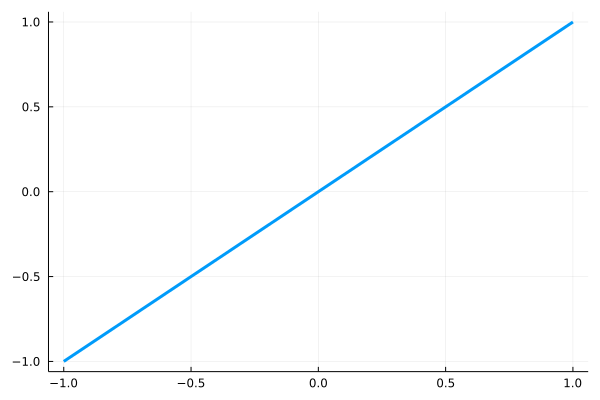
\includegraphics[width=\linewidth]{funciones-activacion/Identidad.png}
        %\end{minipage}
        %\\
        %\hline
         %%%%%%%% Indicadora %%%%%%%
        % Nombre: 
        Indicadora $\lambda \in \R$
        & %expresión 
        $Indicadora_\lambda(x) = 1_{\{x > \lambda\}}$
        & % Rango imagen
        $\{0,1\}$
        & % Gráfica
        \begin{minipage}{\coeficienteAncho\textwidth}
            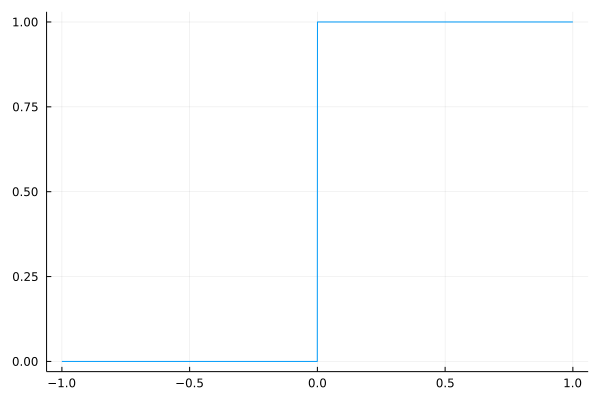
\includegraphics[width=\linewidth]{funciones-activacion/Indicadora de 0.png}
        \end{minipage}
        \\
        \hline
         %%%%%%%% Función umbral %%%%%%%
        % Nombre: 
        Función umbral $p$ polinomio
        & %expresión 
        $Umbral(x) = 1_{\{p(x) > 0\}}$
        & % Rango imagen
        $\{0,1\}$
        & % Gráfica
        \begin{minipage}{\coeficienteAncho\textwidth}
            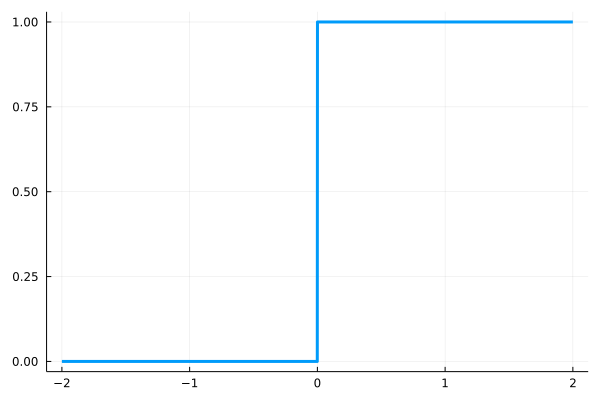
\includegraphics[width=\linewidth]{funciones-activacion/Threshold de polinomio 2x.png}
        \end{minipage}
        \\
        \hline
         %%%%%%%% Función rampa %%%%%%%
        % Nombre: 
        Función rampa
        & %expresión 
        $Rampa(x) = x 1_{\{0 < x <1\}} + 1_{\{x \geq 1\}}$ 
        & % Rango imagen
        $[0,1]$
        & % Gráfica
        \begin{minipage}{\coeficienteAncho\textwidth}
            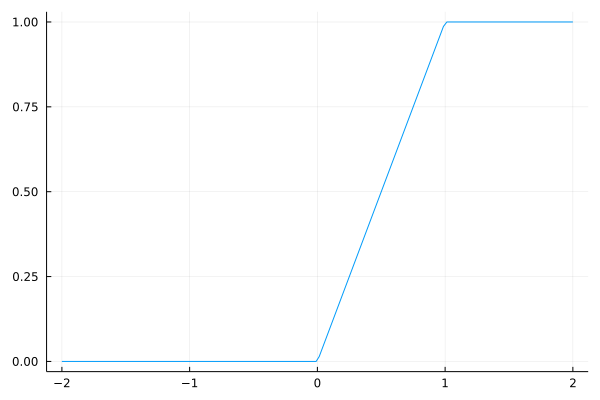
\includegraphics[width=\linewidth]{funciones-activacion/Rampa.png}
        \end{minipage}
        \\
        \hline
        %%%%%%%% sigmoide %%%%%%%%
        % Nombre: 
        Sigmoidea 
        & %expresión 
        $\sigma(x) = \frac{1}{1+e^{-x}}$
        & %Rango imagen
        $(0,1)$
        & % Gráfica
        \begin{minipage}{\coeficienteAncho\textwidth}
            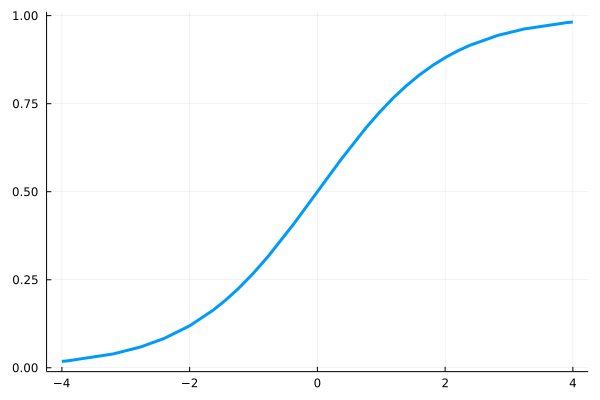
\includegraphics[width=\linewidth]{funciones-activacion/Sigmoid.png}
        \end{minipage}
        \\
        \hline
        %%%%%%%% Tangente hiperbólica  %%%%%%%%
        % Nombre: 
        Tangente hiperbólica 
        & %expresión 
        $\tanh$
        & %Rango imagen
        $(-1,1)$
        & % Gráfica
        \begin{minipage}{\coeficienteAncho\textwidth}
            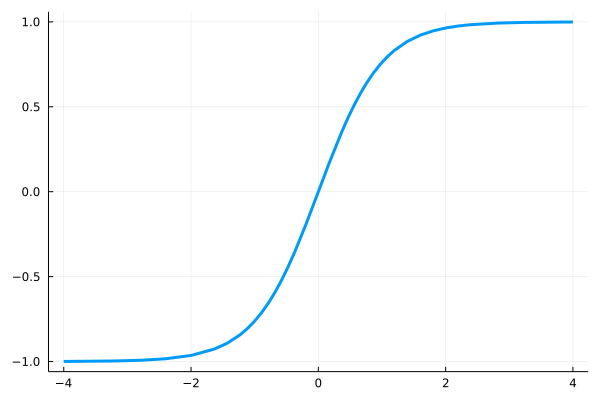
\includegraphics[width=\linewidth]{funciones-activacion/Tangente hiperbolica.png}
        \end{minipage}
        \\
        \hline
        %%%%%%%% Valor absoluto%%%%%%%%
        % Nombre: 
        Valor absoluto
        & %expresión 
        $abs(x)= |x|$
        & %Rango imagen
        $[0,+\infty]$
        & % Gráfica
        \begin{minipage}{\coeficienteAncho\textwidth}
            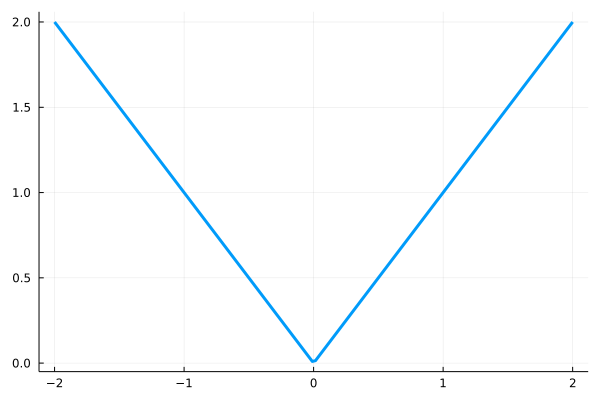
\includegraphics[width=\linewidth]{funciones-activacion/Valor absoluto.png}
        \end{minipage}
        \\
        \hline
         %%%%%%%% Coseno %%%%%%%%
        % Nombre: 
        Coseno
        & %expresión 
        $\cos$
        & %Rango imagen
        $[-1,1]$
        & % Gráfica
        \begin{minipage}{\coeficienteAncho\textwidth}
            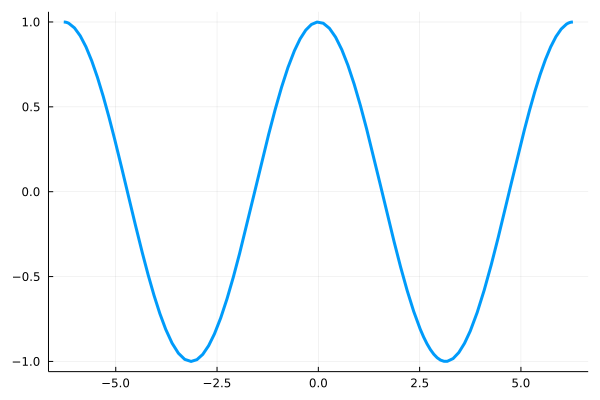
\includegraphics[width=\linewidth]{funciones-activacion/coseno.png}
        \end{minipage}
        \\
        \hline
        %%%%%%%% Cosine Squasher %%%%%%%%
        % Nombre: 
        \textit{Cosine Squasher}
        & %expresión 
        $CosineSquasher(x)=\left(1 + \cos\left(x + 3 \frac{\pi}{2} \right) \frac{1}{2}\right) 
        1_{\{\frac{-\pi}{2} \leq x \leq  \frac{\pi}{2}\}}
        +
        1_{\{ \frac{\pi}{2} < \lambda \}}.$
        & %Rango imagen
        $[0,1]$
        & % Gráfica
        \begin{minipage}{\coeficienteAncho\textwidth}
            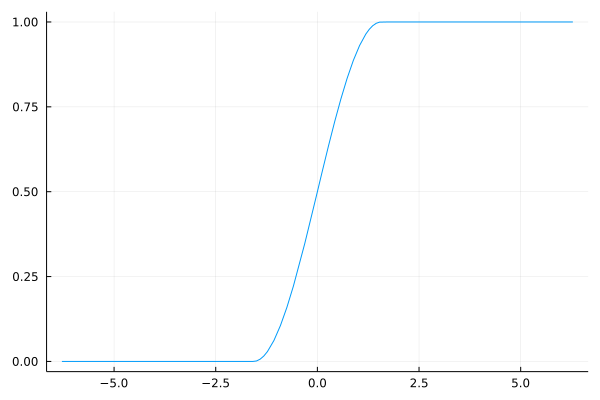
\includegraphics[width=\linewidth]{funciones-activacion/Cosine CosineSquasher.png}
        \end{minipage}
        \\
        \hline
        %%%%%%%% ReLU %%%%%%%%
        % Nombre: 
        \textit{ReLU}
        & %expresión 
        $ReLU(x) = \max(0,x)$
        & %Rango imagen
        $[0,+\infty)$
        & % Gráfica
        \begin{minipage}{\coeficienteAncho\textwidth}
            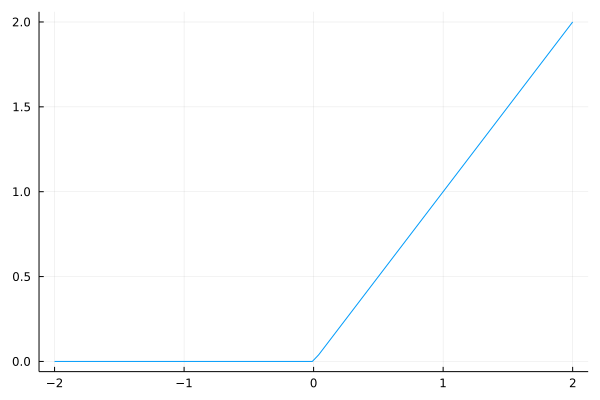
\includegraphics[width=\linewidth]{funciones-activacion/ReLU.png}
        \end{minipage}
        \\
        \hline
        %%%%%%%% Hard Hyperbolic Function %%%%%%%%
        % Nombre: 
        \textit{Hard Hyperbolic Function}
        & %expresión 
        $Hardtanh(x) =\left\{ \begin{array}{lcc}
            -1 &   si  & x \leq -1 \\
            \\ x &  si & -1< x < 1 \\
            \\ 1&  si  & x \geq 1 
            \end{array}
        \right.$
        & %Rango imagen
        $[-1,1]$
        & % Gráfica
        \begin{minipage}{\coeficienteAncho\textwidth}
            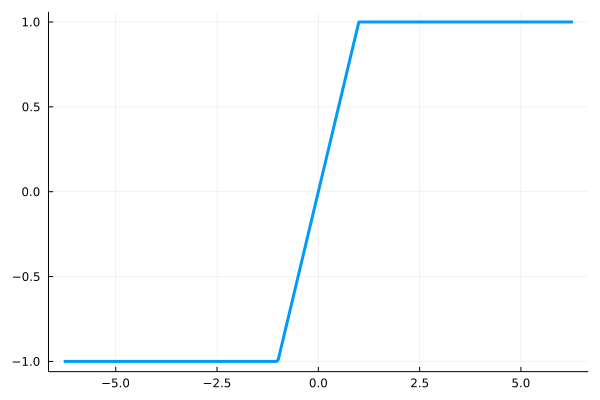
\includegraphics[width=\linewidth]{funciones-activacion/hardtanh.png}
        \end{minipage}
        \\
        \hline
        %%%%%%%% Leaky ReLU%%%%%%%
        % Nombre: 
        \textit{Leaky ReLU}
        & %expresión 
        $\begin{array}{c}

            LReLU_{\alpha}(x) =\left\{ \begin{array}{lcc}
            \alpha x &   si  & x \leq 0 \\
            \\ x&  si  & x > 0 
            \end{array}
            \right.
        \\
        \text{con } \alpha \in \R^+ \text{valor }\textit{pequeño}.
        \end{array}
        $
        & % Rango imagen
        $[0, +\infty)$
        & % Gráfica
        \begin{minipage}{\coeficienteAncho\textwidth}
            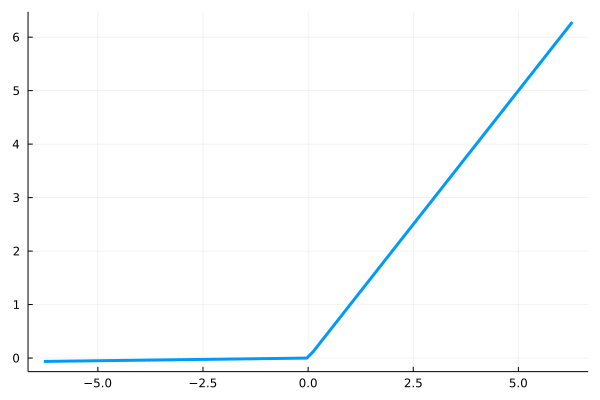
\includegraphics[width=\linewidth]{funciones-activacion/LReLU.png}
        \end{minipage}
        \\
        \hline
    \end{tabular}
    } % fin de llave de ajustarse al ancho de la página
    \caption{Compendio de funciones de activación}  
    \label{table:funciones-de-activation}
\end{table}

% comentario margen
% Qué hace la función afín definida
% y relevancia teorema 
\setlength{\marginparwidth}{\bigMarginSize}
\marginpar{\maginLetterSize
    \iconoAclaraciones \textcolor{dark_green}{     
        \textbf{
            Qué hace la función $\phi$
        }
    }

    Tal función significa aplicar traslaciones,
    simetrías, reescalados  o composiciones de estos
    movimientos a la imagen de la función afín.

    \iconoClave  \textcolor{darkRed}{     
        \textbf{
            Utilidad práctica del teorema
        }
    }

    Gracias a este resultado sabremos 
    cuándo dos funciones de activación 
    producirán exactamente los mismos resultados.
    Por lo tanto podremos seleccionar 
    la más oportuna, por ejemplo 
    la que tenga menos coste.
}


\begin{aportacionOriginal}

\begin{teorema}\label{teo:eficacia-funciones-activation}
    \label{teo:equivalencia-grafos-activation-function}
    Sea $\phi \in \mathcal{A}(\R^2)$ una función afín 
    cuya forma matricial asociada es de la forma:  
    \begin{equation}
        \phi((x,y)) =  
        \begin{bmatrix}
            a & 0 \\
             0& b 
        \end{bmatrix}
        \begin{bmatrix}
            x \\
            y
        \end{bmatrix}
        +
        \begin{bmatrix}
            t_x  & t_y
        \end{bmatrix}
    \end{equation}
    con $a,b \in \R^*$ y $t_x, t_y \in \R$.

    Sean dos funciones de activación $\sigma, \gamma$ tales que 
    \begin{equation*}
        \phi(Grafo(\sigma)) = Grafo(\gamma),
    \end{equation*}
    entonces 
    el espacio de redes neuronales de $n$ neuronas creado con la función de activación $\sigma$ es  
    igual al espacio de redes neuronales creado con la función de activación $\gamma$. 
\end{teorema}
\begin{proof}
    % Primero lo demostramos con sesgo
    Sea $\mathcal{H}^+_{\sigma, n}(\R^d, \R^s)$ el espacio de redes neuronales con $n$ neuronas con sesgo. 

    Está claro que 
    $\mathcal{H}^+_{\gamma, n}(\R^d, \R^s)$ 
        y 
        $\mathcal{H}^+_{\sigma, n}(\R^d, \R^s)$ 
        son biyectivos.
   
    Ya que basta con tomar una red neuronal de una y cambiarle la función de activación por la de la otra. 
    Veamos 
    que se da la igualdad viendo que una está contenida en la otra. 

    Para cualquier $h  \in \mathcal{H}^+_{\sigma, n}(\R^d, \R^s)$
    la proyección i-ésima de $h$ será de la forma 

    \begin{equation*}
        h_i(x) = \sum^n_{j=1}(\beta_{j} \sigma(A_j(x))+ k_j),
    \end{equation*}
    con $x \in \R^d, \beta_{j}, k_j \in \R, A_j \in \afines$. 
    % Se define la h tilda: 
    Procedemos a definir $\tilde{h}_i(x)$ como sigue 
    \begin{align}\label{eq:h-tilda-definition}
        \tilde{h}_i(x) 
        = \sum^n_{j=1}(\beta_{j}  (b \sigma( a A_j(x) + t_x) + t_y)+ k_j)
        = \sum^n_{j=1}(\tilde{\beta}_{j} \sigma(\tilde{A}_j(x))+ \tilde{k_j}),
    \end{align}
    con $x \in \R^d, \tilde \beta_{j}, \tilde k_j \in \R, \tilde{A}_j \in \afines$,
    por lo que está claro que $\tilde{h}(x) \in \mathcal{H}^+_{\sigma, n}(\R^d, \R^s)$. 
 
    Observemos que la 
    hipótesis del enunciado 
    establece que
    \begin{align}
        Grafo(\gamma) &= \{ (x, \gamma(x)) \colon x \in \R \} 
        \\
        & = 
        Grafo(\gamma)  = \phi(Grafo(\sigma)) 
        \\
        & = 
        \phi( \{ (x, \sigma(x)) \colon x \in \R \})
        \\
        &=
        \{ (a x + t_x, b \sigma(x) + t_y) \colon x \in \R \}.
    \end{align}
    Por lo que $\tilde{h}$ así definida (\refeq{eq:h-tilda-definition})
    es a su vez 
    \begin{align}
        \tilde{h}_i(x) 
        = \sum^n_{j=1}(\beta_{j}  \gamma A_j(x)+ k_j)
    \end{align}
     es decir que $\tilde{h}(x) \in \mathcal{H}^+_{\gamma, n}(\R^d, \R^s)$. 
    Así que vía $\phi$ se ha definido una inyección 
    de $\mathcal{H}^+_{\sigma, n}(\R^d, \R^s)$ a 
    $\mathcal{H}^+_{\gamma, n}(\R^d, \R^s)$, 
    esto es 
    \begin{equation}
        \mathcal{H}^+_{\sigma, n}(\R^d, \R^s)
        \subseteq
        \mathcal{H}^+_{\gamma, n}(\R^d, \R^s).  
    \end{equation}

    Además, $\phi$ con las hipótesis exigidas es
    invertible, con inversa: 
    \begin{equation}
        \phi^{-1}((x,y)) =  
        \begin{bmatrix}
            \frac{1}{a} & 0 \\
             0& \frac{1}{b} 
        \end{bmatrix}
        \begin{bmatrix}
            x \\
            y
        \end{bmatrix}
        +
        \begin{bmatrix}
            - \frac{t_x}{a}  &  - \frac{t_y}{b}
        \end{bmatrix}.
    \end{equation}
    Así que razonando de igual manera que en el 
    apartado anterior se tiene la inclusión
    \begin{equation}
        \mathcal{H}^+_{\sigma, n}(\R^d, \R^s)
        \supseteq
        \mathcal{H}^+_{\gamma, n}(\R^d, \R^s),  
    \end{equation}
    por lo que podemos concluir que 
    \begin{equation*}
        \mathcal{H}^+_{\gamma, n}(\R^d, \R^s) 
        = 
        \mathcal{H}^+_{\sigma, n}(\R^d, \R^s).
    \end{equation*}
    
    Como demostramos en \ref{consideration-irrelevancia-sesgo} se tiene que 
    \begin{equation*}
        \mathcal{H}^+_{\sigma, n}(\R^d, \R^s) = \mathcal{H}^+_{\gamma, n}(\R^d, \R^s) 
        \subset 
            \mathcal{H}_{\gamma, n+1}(\R^d, \R^s) 
        \subset
        \mathcal{H}^+_{\gamma, {n+1}}(\R^d, \R^s) = \mathcal{H}^+_{\sigma, {n+1}}(\R^d, \R^s) 
        .
    \end{equation*}
    Por lo que para un $n$ arbitrariamente grande, se acaba de probar lo buscado. 
    \begin{equation*}
        \mathcal{H}_{\gamma}(\R^d, \R^s) = \mathcal{H}_{\sigma}(\R^d, \R^s).
    \end{equation*}
\end{proof}
\end{aportacionOriginal}



\subsubsection*{\iconoClave  \textcolor{darkRed}{Relevancia práctica del teorema}}
Este teorema lo que nos está diciendo es que si dos funciones de activación tienen \textit{la misma forma}
(independientemente de su grafo)
entonces \textbf{aproximarán igual de bien},
es decir, con el mismo error dentro de un conjunto de datos.
 Esto a nivel práctico  significa que \textbf{si se tienen dos funciones de activación
  \textit{con la misma forma} (\textit{o muy parecida}) elige
   la que tenga menor costo computacional}, porque a 
   nivel teórico aproximarán igual de bien y de esta
    manera ahorraremos recursos. 

Notemos además que la demostración nos enseña que la igualdad se da independientemente del número de 
neuronas fijado, es decir que no es un resultado 
asintótico (lo asintótico en términos prácticos 
significa que sea resultado de una serie de 
aproximaciones).  

% Relevancia corolario 
\marginpar{\maginLetterSize
    \iconoAclaraciones \textcolor{dark_green}{     
        \textbf{
            Relevancia corolario 
            \ref{corolario:afine-activation-function}
        }
    }
    Simplifica las comparativas entre funciones 
    de activación 
    sin necesidad de conocer su imagen.
}
%corolario para cuando sean afines 
\begin{corolario}\label{corolario:afine-activation-function}
    Sea $\phi \in \mathcal{A}(\R)$ una transformación afín e invertible, esto es de la forma 
    \begin{equation}
        \phi(x) = a x + b 
        \text{ con } a \in \R^*, b \in \R.
    \end{equation}
    Dadas dos funciones de activación $\sigma$ y $\gamma$ que satisfagan que 
    \begin{equation}
        \phi \circ \sigma = \gamma,
    \end{equation} 
    entonces 
    el espacio de redes neuronales de $n$ neuronas creado con la función de activación $\sigma$ es  
    igual al espacio de redes neuronales creado con la función de activación $\gamma$. 
\end{corolario}
\begin{proof}
    En base a que $\phi(x) = a x + b$, con 
    $a \in \R^*, b \in \R$
    basta con definir 
     $\psi  \in \mathcal{A}(\R^2)$ como 
    \begin{equation}
        \psi((x,y)) =  
        \begin{bmatrix}
            1 & 0 \\
             0& a
        \end{bmatrix}
        \begin{bmatrix}
            x \\
            y
        \end{bmatrix}
        +
        \begin{bmatrix}
            0 & b
        \end{bmatrix}.
    \end{equation}
    A partir  definición se tiene que 
    \begin{align}
        Grafo(\gamma) &=
        \{ (x, \gamma(x)) \colon x \in \R\} 
        \\
        & = 
        \{ (x, \phi(\sigma(x))) \colon x \in \R\}
        \\
        & =
        \psi(\{ (x, \sigma(x)) \colon x \in \R\})
        = 
        \psi(Grafo(\sigma)).
    \end{align}
    Se satisfacen 
    las hipótesis del teorema \ref{teo:equivalencia-grafos-activation-function} y en virtud de él se tiene el resultado buscado.
\end{proof}

\section{ Selección de las mejores funciones de activación}
Así pues, a la vista de la imágenes de las distintas funciones de activación 
recogidas en la tabla \ref{table:funciones-de-activation}, y
por el recién probado teorema \ref{teo:eficacia-funciones-activation}, podemos determinar a priori 
que de manera teórica existen conjuntos de funciones que aproximadamente  pueden producir los mismos resultados. 

A la vista de del resultado, si las funciones de 
activación son similares entonces actuarán con 
una precisión similar, es por ello 
que el la table \ref{table:Clases-equivalencia-activation-function} establecemos 
las siguientes clases de funciones de activación 

\begin{table}[H] 
    \centering  
    \begin{tabular}{| c | c | c | }
        \hline
        \textit{Grupo escalera} & \textit{Grupo sigmoide} & \textit{Grupo ReLU} \\
        \hline
       &  Rampa &  \\
       Indicadora & Sigmoidea & ReLU\\
       Umbral & \textit{Cosine Squasher}& LReLU\\
        & tanh & \\
        & \textit{Hard Hyperbolic Function}& \\
\hline
    \end{tabular}
    \caption{Agrupaciones de funciones de activación con forma similar}  
    \label{table:Clases-equivalencia-activation-function}
\end{table}

Compararemos entonces su coste computacional y tomaremos como representante de la clase aquel que sea de menor coste. 


\subsection{ Implementación de las funciones de activación en la biblioteca de redes neuronales} 
\label{ch06:activation-function-implementation}
Las funciones de activación han sido implementadas con cuidado de que sean eficientes 
y valiéndose de las características propias de Julia, para ello se han utilizado técnicas como: 

% Comentario aclaratorio de qué es indirección 
\setlength{\marginparwidth}{\bigMarginSize}
\marginpar{\maginLetterSize
    \iconoAclaraciones \textcolor{dark_green}{     
        \textbf{
            Significado indirección 
        }
    }

    La indirección es una técnica de programación 
    que consiste en hacer una referencia indirecta 
    a los datos usando direcciones en memoria. 
    Esto conlleva el almacenamiento en memoria no solo 
    de los datos, si no de las direcciones (que no deja de ser un dato más).   
}

% Comentario aclaratorio de qué es indirección 
\marginpar{\maginLetterSize
    \iconoAclaraciones \textcolor{dark_green}{     
        \textbf{
            Significado \textit{overhead}
        }
    }

    Hace referencia a el coste  computacional adicional 
    que conllevan resolver las indirecciones en este caso.
}

\begin{itemize}
    % Programación modular 
    \item \textbf{Programación modular}: Tal y como se recomienda en la documentación de Julia \footnote{
        Consultada en la página web oficial de Julia  a día 23 de mayo del 2022 con URL: \url{https://docs.julialang.org/en/v1/manual/modules/}
    } se ha utilizado un módulo en la implementación de la biblioteca, esto aporta los siguientes beneficios: 
    \begin{itemize}
        \item Los módulos pueden ser precompilados y de esta manera se aceleraría la carga y el tiempo de inicialización. 
        \item Encapsulamiento de los métodos y facilidades de uso del espacio de nombres, lo cual forma parte
        de una buena metodología de programación. 
    \end{itemize}

    % Macros
    \item \textbf{Macros}\footnote{La información consultada de macros ha sido  de la página oficial de Julia, a día 23 de mayo del 2022, URL:
    \url{https://docs.julialang.org/en/v1/manual/metaprogramming}}:
    que permiten sustituciones de código cuando el código es analizado por el compilador; 
    de esta manera, funciones que devuelven otras funciones dependientes de un parámetro se verán beneficiadas,
    ya que hace que se ejecute código más rápido evitando indirecciones \footnote{La fuente bibliográfica ha sido la \href{https://es.wikipedia.org/wiki/Indirección}{Wikipedia}, a día 26 de mayo del 2022.
    También recomendamos especialmente la entrada en inglés de la misma:
    \href{https://en.wikipedia.org/wiki/Indirection}{\textit{Indirection}}
    consultada también el día 26 de mayo del 2022.
    }  y el y el overhead correspondiente. 
     Puede encontrar la implementación de esto en la biblioteca de redes neuronales implementada en nuestro 
     repositorio 
     \footnote{
         Esto es en \url{https://github.com/BlancaCC/TFG-Estudio-de-las-redes-neuronales/tree/main/OptimizedNeuralNetwork.jl/src/activation_functions.jl}
     }.

     % Funtores 
     \item Funtores o como son llamados en Julia \href{https://docs.julialang.org/en/v1/manual/methods/#Function-like-objects}{\textit{Function-like objects}}. Junto con las macros son una forma eficiente definir funciones de funciones y valores por defecto. 
\end{itemize}

Además la implementación de la biblioteca se ha hecho de acorde 
al \textbf{principio de sustitución de Liskov} (publicado en el artículo \cite{Liskov-principle}) que dice así: 

\enquote{
    Sea $\phi(x)$ una propiedad comprobable acerca de los objetos $x$ de tipo $T$. 
    Entonces $\phi(y)$  debe ser verdad para los objetos $y$ del tipo $S$, donde $S$ es un 
    subtipo de $T$. 
}

Esto significa que todas deben de comportarse
como una función de activación abstracta y poder intercambiarse entre ellas. 
Lo que en un principio suena obvio, ha supuesto un diseño cuidadoso y un uso de las herramientas que brinda Julia en toda 
su plenitud, puesto que tengamos en cuenta que la variabilidad a la hora de definir y caracterizar a una función de activación, ya que algunas no dependen de ningún parámetro 
mientras que otras lo hacen incluso de otras funciones (ver definiciones en la tabla \ref{table:funciones-de-activation}). 

 
    % Sistema de tipos
\subsubsection*{Sobre el sistema de tipos de Julia}
\label{ch06:sistema-timpos-julia}
    Julia posee un sistema de tipos muy rico 
    \footnote{
        Véase la documentación oficial de Julia sobre \textit{Types}: 
        \url{https://docs.julialang.org/en/v1/manual/types/}. 
        Esta URL fue consultada el 26 de mayo de 2022.
    }
    dinámico, nominal y paramétrico; pero que ofrece la posibilidad de obtener
    beneficio de los tipos estáticos.
    Podría entonces un plantearse 
    Sacar provecho de esto en la \textcolor{darkRed}{declaración 
    del dominio} e imagen de una función de activación y prevención de errores. 
 
    % Nota sobre porqué nos interesa ajustar el dominio
    \reversemarginpar
    \setlength{\marginparwidth}{\smallMarginSize}
    \marginpar{\maginLetterSize
    \iconoClave \textcolor{darkRed}{     
        \textbf{
            Interés de controlar el dominio de una función
        }
    } 

    Lo cual permitiría optimizar la evaluación de la función; 
    ya que si la función tuviera comportamientos diferentes en función del rango, 
    habría que estudiarlos con condiciones interiores que aumentan el costo computacional.
    }
    \setlength{\marginparwidth}{\bigMarginSize}
    \normalmarginpar 
    % fin de la nota, comienza explicación 
   
    % Nota en margen sobre tipos estáticos y dinámicos 
    \marginpar{\maginLetterSize
    \iconoAclaraciones \textcolor{dark_green}{     
        \textbf{
            Tipos estáticos y dinámicos
        }
    }

    El tipo de dato \textbf{estático} se define en memoria 
    antes de la ejecución del código (durante la compilación del código),
     no pudiendo cambiar 
    durante la ejecución del programa. 
    
    Un tipo de dato \textbf{dinámico} puede cambiar y el tipo es determinado mediante 
    la ejecución. 

    Por lo general las ventajas del estático son mayor eficiencia y prevención de errores,
    por el contrario, tipos dinámicos permiten más flexibilidad a la hora de diseñar 
    y escribir el código. 
    }
    % Nota en margen sobre tipos nominal 
    \marginpar{\maginLetterSize
    \iconoAclaraciones \textcolor{dark_green}{     
        \textbf{
            Tipo de dato nominal
        }
    }
    Dos tipos de datos diferentes serán equivalentes o compatibles, 
    si y solo si se ha hecho de manera explícita. 
    Por ejemplo si definiéramos un tipo de datos de número real y otro de número 
    racional, solo podríamos sumarlos si le explicáramos al ordenador cómo hacerlo. 
    }
     % Nota en margen sobre tipos paramétricos 
     \marginpar{\maginLetterSize
     \iconoAclaraciones \textcolor{dark_green}{     
         \textbf{
             Tipos de datos paramétricos 
         }
     }
     Hace referencia al polimorfismo paramétrico, 
     esto es que una misma función se puede programar 
     para que actúe en consecuencia al tipo de datos que recibe 
     como argumento. 
     }

    Ante esta situación hemos determinado que el tipo más conveniente es a usar en nuestras 
    implementaciones es el racional; ya que como
    procedemos a explicar un tipo más restrictivo
    plantea los siguientes problemas:  

     \begin{itemize}
         \item Los datos se conocen en tiempo real, luego no es posible discriminar su tipo en tiempo de compilación. La única hipótesis que tenemos de los mismos es que son racionales.  
         
         \item En caso de determinar su tipo en tiempo real estaríamos trasladando la 
         condición de rango que queríamos evitar
         a otro lugar de la implementación, 
         por lo tanto seguiría existiendo tal coste. 
         
        \item En nuestra implementación concreta solo beneficiaría a la función de activación \textit{HardTanh} y su implementación no sería satisfactoria porque no habría forma de implementar eficientemente el rango. Ejemplificamos lo que se quiere decir en el código que mostramos a continuación: 
        \begin{itemize}
            \item Entre las líneas 1 y 9 puede verse cómo definir un tipo de dato dominio en Julia.
            \item Entre las líneas 11-13 y las 16-18 cómo se declaran funciones en dominios concretos. 
            \item La línea 14 daría error, la hemos dejado para mostrar que no es posible una declaración de rangos que cumpla el principio de sustitución de Liskov y adapte eficientemente los rangos indicados.
        \end{itemize}
         
     \end{itemize}

     \begin{minipage}{\textwidth}%
     \begin{minted}
        [
        frame=lines,
        %framesep=2mm,
       % baselinestretch=1.2,
        %bgcolor=sutilGreen, 
        linenos
        ]{Julia}
        struct IntervaloCentral{T<:Real} <: Real
        x::T
        function IntervaloCentral{T}(x::T) where T<:Real
            if(-1 > x || x > 1)
                error("No está en intervalo")
            end
            new(x)
        end
    end
    
     function HardTanh(x::IntervaloCentral)
        x.x
    end
    HardTanh(x::Real)=HardTanh(convert(::IntervaloCentral,x))
    
     function HardTanh(x::Real)::Int
        sign(x)
    end
     \end{minted}
\end{minipage} 


\subsection{Coste computacional funciones activación }
\label{ch06:coste-computacional-funciones-activacion}

\subsubsection{Diseño del experimento}
El experimento para comparar los resultados ha consistido en: 
Se ha evaluado cada función a comparar $20.000.000$ veces y se ha medido cuanto tarda. 
Esto se ha repetido $15$ veces. Puede encontrar la implementación concreta y los resultados concretos de cada iteración en el repositorio del
proyecto \footnote{En el directorio de experimentos 
de \url{https://github.com/BlancaCC/TFG-Estudio-de-las-redes-neuronales}.}.
Además, puesto que las funciones más simples que se pueden construir son la identidad y la constante, las hemos añadido para poder comparar el costo. 

\subsubsection{Test de hipótesis}

Compararemos si los resultados son significativos utilizando la \textbf{prueba de los rangos con 
signo de Wilcoxon} (véase \cite{OpenIntroStatistics}, \cite{BiologicalStatistics}, o la web de \href{https://www.cienciadedatos.net}{cienciadedatos.net} \footnote{
 Prueba de los rangos con signo de Wilcoxon by Joaquín Amat Rodrigo, available under a Attribution 4.0 International (CC BY 4.0) at
  \url{https://www.cienciadedatos.net/documentos/18_prueba_de_los_rangos_con_signo_de_wilcoxon}
  Con fecha de visita el 22 de mayo del 2022.
  }).

  La motivación de realizar esta prueba es la siguiente: 
\begin{itemize}
    \item Las muestras son independientes.
    \item Los datos tomados permiten ser ordenados. 
    \item El tamaño de muestra es pequeño y no podemos asegurar normalidad de la datos. 
\end{itemize}

\subsubsection*{Hipótesis} 

\begin{itemize}
    \item $H_0$: La mediana de las diferencias de cada par de datos es $0$. 
    \item $H_a$: La mediana de las diferencias entre cada par de datos es diferente de cero. 
\end{itemize}

La utilidad de este test es que si rechaza la hipótesis nula sabremos que con un $95 \%$ de certeza tendrán medianas diferentes, es decir, \textbf{existe una 
diferencia de tiempos}. En caso de que no se rechace no podremos afirmar nada.
Puede encontrar la implementación en el repositorio del
 proyecto \footnote{En el directorio de experimentos 
 de \url{https://github.com/BlancaCC/TFG-Estudio-de-las-redes-neuronales}.}.

 Los resultados del test de Wilcoxon han sido los siguientes: 

 \begin{table}[H]
    \resizebox{\textwidth}{!}{
    \begin{tabular}{|l|l|l|l|l|l|}
    \hline
        ~ & cte 1  & Identidad  & Umbral de $2x$ & CosineSquasher & Indicadora de 0 \\ \hline
        cte 1  & - &\textbf{No rechaza $H_0$} & Rechaza $H_0$ & Rechaza $H_0$ & Rechaza $H_0$ \\ \hline
        Identidad  & \textbf{No rechaza $H_0$} & - & Rechaza $H_0$ & Rechaza $H_0$ & Rechaza $H_0$ \\ \hline
        Umbral de $2x$ & Rechaza $H_0$ & Rechaza $H_0$ & - & Rechaza $H_0$ & \textbf{No rechaza $H_0$} \\ \hline
        CosineSquasher & Rechaza $H_0$ & Rechaza $H_0$ & Rechaza $H_0$ & - & Rechaza $H_0$ \\ \hline
        Indicadora de 0 & Rechaza $H_0$ & Rechaza $H_0$ & \textbf{No rechaza $H_0$} & Rechaza $H_0$ & - \\ \hline
        Rampa & Rechaza $H_0$ & Rechaza $H_0$ & \textbf{No rechaza $H_0$} & Rechaza $H_0$ & Rechaza $H_0$ \\ \hline
        ReLU & Rechaza $H_0$ & Rechaza $H_0$ & \textbf{No rechaza $H_0$} & Rechaza $H_0$ & \textbf{No rechaza $H_0$} \\ \hline
        Sigmoidea& Rechaza $H_0$ & Rechaza $H_0$ & Rechaza $H_0$ & Rechaza $H_0$ & Rechaza $H_0$ \\ \hline
        Tangente hiperbólica & Rechaza $H_0$ & Rechaza $H_0$ & Rechaza $H_0$ & Rechaza $H_0$ & Rechaza $H_0$ \\ \hline
        Valor absoluto & Rechaza $H_0$ & Rechaza $H_0$ & Rechaza $H_0$ & Rechaza $H_0$ & Rechaza $H_0$ \\ \hline
        Coseno & Rechaza $H_0$ & Rechaza $H_0$ & Rechaza $H_0$ & Rechaza $H_0$ & Rechaza $H_0$ \\ \hline
        Hardtanh & Rechaza $H_0$ & Rechaza $H_0$ & Rechaza $H_0$ & Rechaza $H_0$ & Rechaza $H_0$ \\ \hline
        LReLU & Rechaza $H_0$ & Rechaza $H_0$ & \textbf{No rechaza $H_0$} & Rechaza $H_0$ & \textbf{No rechaza $H_0$} \\ \hline
    \end{tabular}
    }
    \caption{Resultados 1 de 3: Rechazos con un $95\%$ de confianza en el test Wilcoxon.}
    \label{Rechazo-1-de-3}
\end{table}

\begin{table}[H]
    \resizebox{\textwidth}{!}{
    \begin{tabular}{|l|l|l|l|l|}
    \hline
        ~ & Rampa & ReLU & Sigmoidea& Tangente hiperbólica \\ \hline
        cte 1  & Rechaza $H_0$ & Rechaza $H_0$ & Rechaza $H_0$ & Rechaza $H_0$ \\ \hline
        Identidad  & Rechaza $H_0$ & Rechaza $H_0$ & Rechaza $H_0$ & Rechaza $H_0$ \\ \hline
        Umbral de $2x$ & \textbf{No rechaza $H_0$} & \textbf{No rechaza $H_0$} & Rechaza $H_0$ & Rechaza $H_0$ \\ \hline
        CosineSquasher & Rechaza $H_0$ & Rechaza $H_0$ & Rechaza $H_0$ & Rechaza $H_0$ \\ \hline
        Indicadora de 0 & Rechaza $H_0$ & \textbf{No rechaza $H_0$} & Rechaza $H_0$ & Rechaza $H_0$ \\ \hline
        Rampa & - & \textbf{No rechaza $H_0$} & Rechaza $H_0$ & Rechaza $H_0$ \\ \hline
        ReLU & \textbf{No rechaza $H_0$} & - & Rechaza $H_0$ & Rechaza $H_0$ \\ \hline
        Sigmoidea& Rechaza $H_0$ & Rechaza $H_0$ & - & Rechaza $H_0$ \\ \hline
        Tangente hiperbólica & Rechaza $H_0$ & Rechaza $H_0$ & Rechaza $H_0$ & - \\ \hline
        Valor absoluto & Rechaza $H_0$ & Rechaza $H_0$ & Rechaza $H_0$ & Rechaza $H_0$ \\ \hline
        Coseno & Rechaza $H_0$ & Rechaza $H_0$ & Rechaza $H_0$ & Rechaza $H_0$ \\ \hline
        Hardtanh & Rechaza $H_0$ & Rechaza $H_0$ & Rechaza $H_0$ & Rechaza $H_0$ \\ \hline
        LReLU & \textbf{No rechaza $H_0$} & \textbf{No rechaza $H_0$} & Rechaza $H_0$ & Rechaza $H_0$ \\ \hline
    \end{tabular}
    }
    \caption{Resultados 2 de 3: Rechazos con un $95\%$ de confianza en el test Wilcoxon.}
    \label{Rechazo-2-de-3}
\end{table}

\begin{table}[H]
    \resizebox{\textwidth}{!}{
    \begin{tabular}{|l|l|l|l|l|}
    \hline
        ~ & Valor absoluto & Coseno & Hardtanh & LReLU \\ \hline
        cte 1  & Rechaza $H_0$ & Rechaza $H_0$ & Rechaza $H_0$ & Rechaza $H_0$ \\ \hline
        Identidad  & Rechaza $H_0$ & Rechaza $H_0$ & Rechaza $H_0$& Rechaza $H_0$ \\ \hline
        Umbral de $2x$ & Rechaza $H_0$ & Rechaza $H_0$ & Rechaza $H_0$ & \textbf{No rechaza $H_0$} \\ \hline
        CosineSquasher & Rechaza $H_0$ & Rechaza $H_0$ & Rechaza $H_0$ & Rechaza $H_0$ \\ \hline
        Indicadora de 0 & Rechaza $H_0$ & Rechaza $H_0$ & Rechaza $H_0$ & \textbf{No rechaza $H_0$} \\ \hline
        Rampa & Rechaza $H_0$& Rechaza $H_0$ & Rechaza $H_0$ & \textbf{No rechaza $H_0$} \\ \hline
        ReLU & Rechaza $H_0$ & Rechaza $H_0$ & Rechaza $H_0$ & \textbf{No rechaza $H_0$} \\ \hline
        Sigmoidea& Rechaza $H_0$ & Rechaza $H_0$ & Rechaza $H_0$ & Rechaza $H_0$ \\ \hline
        Tangente hiperbólica & Rechaza $H_0$ & Rechaza $H_0$ & Rechaza $H_0$ & Rechaza $H_0$ \\ \hline
        Valor absoluto & - & Rechaza $H_0$ & Rechaza $H_0$ & \textbf{No rechaza $H_0$} \\ \hline
        Coseno & Rechaza $H_0$ & - & Rechaza $H_0$ & Rechaza $H_0$ \\ \hline
        Hardtanh & Rechaza $H_0$ & Rechaza $H_0$ & - & Rechaza $H_0$ \\ \hline
        LReLU & Rechaza $H_0$ & \textbf{No rechaza $H_0$} & Rechaza $H_0$ & - \\ \hline
    \end{tabular}
    }
    \caption{Resultados 3 de 3: Rechazos con un $95\%$ de confianza en el test Wilcoxon.}
    \label{Rechazo-3-de-3}
\end{table}

Como ya comentábamos, si la hipótesis nula es rechazada podemos suponer que hay una diferencia 
de tiempo significativa;  en caso contrario no podemos saber nada. 

Sin embargo, podemos entender estos rechazos como una clase de equivalencia; es decir, la diferencia en coste computacional no es tan significativa, dentro de ese grupo. De hecho, como podemos apreciar en la tabla \ref{Tiempos-ejecucion-comparativas}, que está ordenada de menor tiempo a mayor,
 estos se encuentran en posiciones consecutivas y en los mismos rango de tiempos de la respectiva
 gráfica de caja y bigote figura \ref{img:boxplot-whiskers-activation-function}.

\begin{table}[H]
    \centering
    \resizebox{0.8\textwidth}{!}{  
    \begin{tabular}{|l|c |c|}
    \hline
        Función & Mediana & Media tiempo  \\ \hline
        cte 1 (para comparar) & 1475,959 & 1473,478 $\pm$ 26,332 \\ \hline
        Identidad (para comparar) & 1479,817 & 1467,311 $\pm$ 27,021 \\ \hline
        Hardtanh & 1495,105 & 1491,046 $\pm$ 21,334 \\ \hline
        CosineSquasher & 1522,128 & 1521,117 $\pm$ 19,223 \\ \hline
        ReLU & 1546,379 & 1552,049 $\pm$ 21,435 \\ \hline
        Indicadora de 0 & 1554,432 & 1556,114 $\pm$ 21,814 \\ \hline
        Rampa & 1557,449 & 1552,169 $\pm$ 25,043 \\ \hline
        Umbral de $2x$ & 1562,809 & 1556,669 $\pm$ 23,029 \\ \hline
        LReLU & 1564,124 & 1561,367 $\pm$ 21,722 \\ \hline
        Valor absoluto & 1583,266 & 1580,545 $\pm$ 23,464 \\ \hline
        Sigmoid & 1608,797 & 1601,079 $\pm$ 21,938 \\ \hline
        Coseno & 1630,392 & 1629,634 $\pm$ 26,113 \\ \hline
        Tangente hiperbólica & 1664,006 & 1653,295 $\pm$ 23,025 \\ \hline
    \end{tabular}
    }
    \caption{Tiempo de ejecución en segundos}
    \label{Tiempos-ejecucion-comparativas}
\end{table}

\begin{figure}[H]
    \centering
     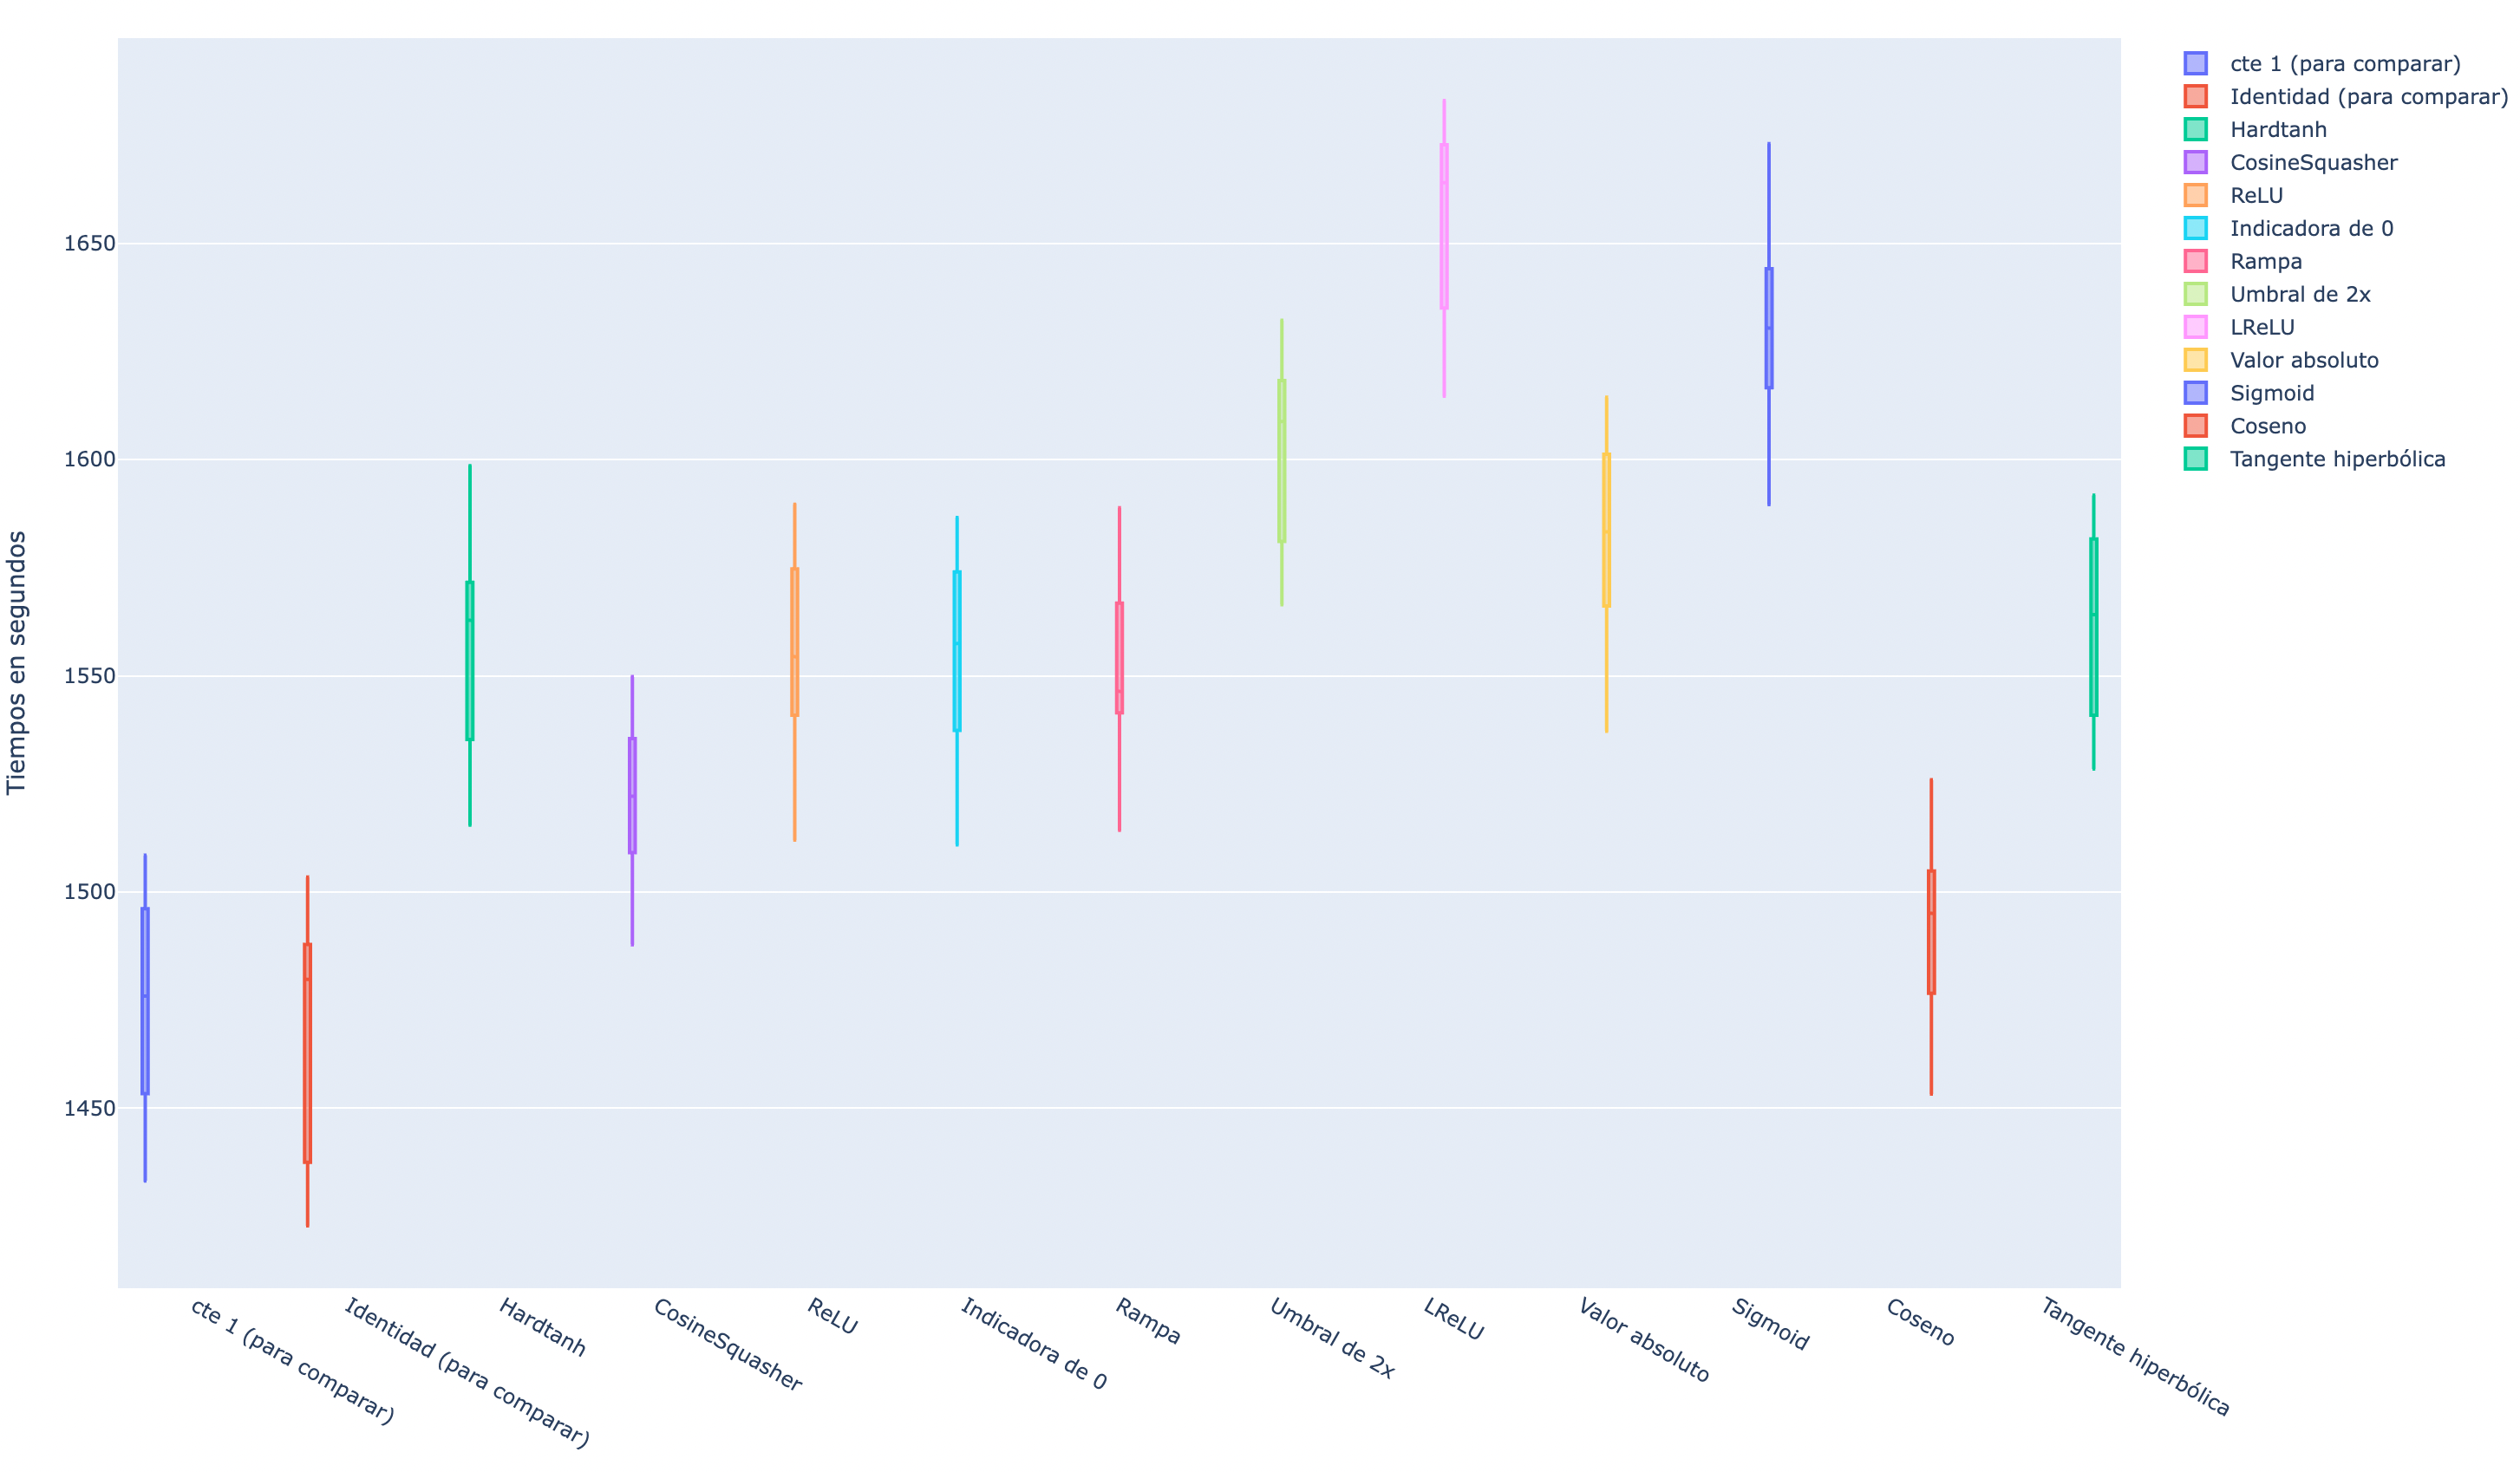
\includegraphics[width=\textwidth]{5-estudio-experimental/activation-function/boxplot-whiskers-activation-function.png}
     \caption{Gráfico de cajas y bigotes con los tiempo de las respectivas funciones}
     \label{img:boxplot-whiskers-activation-function}
\end{figure} 

Si volvemos a nuestro objetivo, que era encontrar el representante de 
menor costo entre las agrupaciones dispuestas en la tabla \ref{table:Clases-equivalencia-activation-function}. Concluimos que los mejores candidatos son: 

\begin{itemize}
    \item Para el \textit{grupo escalera}: No se ha rechazado la hipótesis nula, luego a priori no hay deferencia significativa y podemos seleccionar el candidato que queramos. 
    \item Para el \textit{grupo sigmoide}: La mejor opción ha sido \textit{Hard Hyperbolic Function} y  después en orden de mejor a peor: \textit{Cosine Squasher}, rampa, sigmoidea y tangente hiperbólica.
    \item Pare el \textit{grupo ReLU}: No se ha rechazado la hipótesis nula, así que no podemos decir nada. 
\end{itemize}


% Estudio del algoritmo de inicialización de pesos 
%%%%%%%%%%%%%%%%%%%
%% Optimización de la inicialización de los pesos de una red neuronal 
%%%%%%%%%%%%%%%%%%%%%%%%%
\chapter{ Mejora en la inicialización de los pesos de una red neuronal}  
\label{section:inicializar_pesos}

Como observábamos en la sección \ref{sec:gradiente-descendente}, el gradiente descendente pretende en cada 
iteración mejorar la solución encontrada, pero es 
totalmente sensible a la posición inicial 
de los pesos. 
Presentamos por tanto una propuesta para 
inicializar una red neuronal con el objetivo de que 
sus pesos se encuentren ya cerca de la solución. 
Destaquemos que este algoritmo 
no solo servirá exclusivamente para el método de gradiente descendente 
sino para cualquier otro dependiente del punto inicial. 

\section*{Contenido y objetivo del capítulo}  

\begin{itemize}
    \item Establecimiento del estado del arte en \ref{ch07:estado-arte}.
    \item Descripción del algoritmo y demostración de su corrección \ref{ch07:algoritmo-propuesto}.
    \begin{itemize}
        \item Determinación de su complejidad algorítmica. 
        \item Selección de parámetros y generalización. 
    \end{itemize}
    \item Descripción de la implementación. 
    \item Beneficios obtenidos.  
\end{itemize}



\section{ Estado del arte relacionado } 
\label{ch07:estado-arte}
% Nota informativa de lo que es un backbone 
\setlength{\marginparwidth}{\bigMarginSize}
\marginpar{\maginLetterSize
    \iconoAclaraciones \textcolor{dark_green}{     
        \textbf{
            Qué es un \textit{backbone}
        }
    }

    Se denomina \textit{backbone} a los nodos de una red neuronal que han sido \textbf{inicializados con valores 
    de otras redes neuronales ya entrenadas}. Por ejemplo si quisiéramos clasificar insectos y partiéramos de una red neuronal que se entrenó para clasificar frutas.  
    
}

Se ha comprobado en la práctica que el uso de 
\textit{backbones} reporta mejoras sustanciales en el 
entrenamiento de redes neuronales, véanse artículos como \cite{backbone-object-detection}, \cite{backbone-Architecture} y sus referencias. 

Cuando se carece de \textit{backbones} o no es posible utilizarlos, una buena técnica para dar un valor inicial  a los pesos consiste en basarse en metaheurísticas tales como algoritmos genéticos,
ver \cite{Montana2002NeuralNW}, sin embargo, éstos 
tienen un coste computacional importante. 

Ante esta situación, nuestro algoritmo propone una inicialización de bajo coste computacional y que no necesita de más valores que los del conjunto de entrenamiento. 



\section{Descripción del método propuesto}
\label{ch07:algoritmo-propuesto}
\begin{aportacionOriginal} % método de construción
    
La idea proviene de la demostración casi constructiva del teorema \ref{teorema:2_5_entrenamiento_redes_neuronales}.

Se desea inicializar los pesos de $h \in \rrnnsmn$, para la cual, una vez fijado el número $n$ de neuronas de nuestra red neuronal, será necesario  determinar un subconjunto $\Lambda \mathcal{D}$ de datos de entrenamiento. 

La bondad del resultado depende en gran medida de $\Lambda$, 
puesto que a priori se carece de hipótesis, se seleccionará 
de manera aleatoria bajo el supuesto de una distribución 
independiente e idénticamente distribuida de los datos. 

Como apunta la demostración, debe encontrarse un 
$p \in \R^d$ satisfaciendo que $p \cdot (x_i-x_j) \neq 0$ para cualesquiera
atributos $x_i,x_j$ distintos de $\Lambda$.  

Es decir que se estaría considerando un vector que no 
pertenezca a una unión finita de hiperplanos ortogonales de $\R^r$. 
De manera teórica la probabilidad de seleccionar un $p$ y 
que pertenezca al espacio ortogonal es $0$, sin embargo esto 
no quiere decir que no pueda pasar. 

Tomaremos por tanto un $p$ aleatorio y a partir de él 
seleccionaremos $\Lambda$ lo suficientemente grande para que
 al menos $n$ vectores admitan de manera estricta la ordenación: 

\begin{equation}\label{eq:method_inicializar_condition_desigualdad}
    p \cdot x_1 < 
    p \cdot x_2 
    < \cdots <
    p \cdot x_n.
\end{equation}
Para continuar, para la función de activación 
seleccionada $\gamma$, por cómo se definen 
existirá un $M \in \R^+$ tal que 
\begin{equation} \label{eq:method_inicializar_M}
    \gamma(K)=1 \text{ y } \gamma(-K)=0 
    \text{ sean constantes para todo }K \geq M.
\end{equation}

Una vez concretados los valores $p$, $\Lambda$ y $M$ que satisfagan las condiciones 
(\refeq{eq:method_inicializar_condition_desigualdad}) 
y (\refeq{eq:method_inicializar_M})  
falta concretar los valores iniciales de la red neuronal. 

Para ello debemos calcular el valor de las matrices $(A,S,B)$ que definen a una red neuronal y que presentamos en la sección \ref{section:rrnn_implementation}.

Recordemos que $A$ y $S$ tienen tantas filas como neuronas  y $B$ tantas columnas como neuronas. 

Usado la notación vectorial
$p_{[i,j]} = (p_i, p_{i+1}, \ldots, p_{j})$ donde $(p_0, p_1, \ldots, p_d)=p$, comenzaremos definiendo el valor de la primera fila como

\begin{align}
    &S_1 = M p_0, \\
    & A_{1 *} = M p_{[1,d]}, \\
    & B_{* 1} = y_1.
\end{align}

Los valores de la fila  k-ésima de las matrices $(A,S)$, vendrán determinados por la única función afín $A \in \afines$, 
dada por $A_k(x)=B_k(p \cdot x)$, con $B_{k}$ como la única función afín de $\R$ en $\R$ que cumple que 
\begin{equation}
    B_k(p \cdot x_{k-1}) = -M 
    \quad \text{y} \quad 
     B_{k}(p \cdot x_k)= M.
\end{equation}

Esto equivale a calcular las constantes reales $\tilde {\alpha}$. 

Si tenemos presente que 
\begin{equation}
    \tilde{\alpha}_{k p} (p \cdot x_{k-1}) + \tilde{\alpha}_{k s} = -M 
    \quad \text{y} \quad 
    \tilde{\alpha}_{k p}(p \cdot x_k) + \tilde{\alpha}_{k s}= M.
\end{equation} 
Resolviendo el sistema resulta que 

\begin{equation}
    \left\{ 
        \begin{array}{l}
            \tilde{\alpha}_{k p} = \frac{2 M}{p \cdot (x_k - x_{k-1})}
            \\
            \tilde{\alpha}_{k s} 
            = M -  \tilde{\alpha}_{k p}(p \cdot x_{k})
            = M -  \frac{2 M}{p \cdot (x_k - x_{k-1})}(p \cdot x_{k}) 
        \end{array}
    \right.
\end{equation}

Luego los coeficientes de la red neuronal $A$, $S$ se deducirían de 
\begin{equation}
    \left\{ 
        \begin{array}{l}
            \alpha_{k 0} = \tilde{\alpha}_{k s} =
            M -  \frac{2 M}{p \cdot (x_k - x_{k-1})}(p \cdot x_{k}) 
            \\
            \alpha_{k i} =  \tilde{\alpha}_{k p} p_{i}
            = 
            \frac{2 M}{p \cdot (x_k - x_{k-1})}
            p_i 
        \end{array}
        \right.
\end{equation}

Esto define un sistema lineal compatible
cuya solución son las respectivas filas y columnas: 

\begin{equation}
    \left\{ 
        \begin{array}{l}
            S_{k} = M -  \frac{2 M}{p \cdot (x_k - x_{k-1})}(p \cdot x_{k-1})\\
            A_{k i} = \frac{2 M}{p \cdot (x_k - x_{k-1})}
            p_{i}  
            \\
            B_{* k} = y_k - y_{k-1}
        \end{array}
    \right.
\end{equation}  
\end{aportacionOriginal} % método de construcción

Con todo esto el proceso algorítmico resultante es: 

% Algoritmo de inicialización de pesos de una red neuronal
\begin{algorithm}[H]
    \caption{Inicialización de pesos de una red neuronal}
    \label{algo:algoritmo-iniciar-pesos}
    \textbf{Input:} Tamaño red neuronal $n$, conjunto de datos de entrenamiento $\mathcal{D}$, constate $M$ involucrada en \refeq{eq:method_inicializar_M}.

    \textbf{Input:} Red neuronal, representada con las matrices $(A,S,B)$.
    \hspace*{\algorithmicindent} 
    \begin{algorithmic}[1]
        %selección de p
       \STATE \textit{Inicializamos $p$}. \\
       $p \gets$ vector de $\R^{d+1}$. 
       \COMMENT{Como heurística será generado con distribución uniforme en $[0,1]^{d+1}$} 
       % Cálculo de Lambda
       \STATE \textit{Selección  de los datos de inicialización
       $\Lambda \subset \mathcal{D}$}. \\
       \begin{equation}
           \Lambda \gets \{ \emptyset \}
       \end{equation}
       \While{tamaño de $\Lambda < n$}{
            Tomamos de manera aleatoria $(x,y)$ de $\mathcal{D}$.   \\
        \If{para todo $(a,b) \in \Lambda$ se satisface que 
        $p \cdot (x-a) \neq 0$}{ 
           \begin{equation}
                \Lambda  \gets \Lambda \cup \{(x,y)\}.
           \end{equation} 
           \COMMENT{$\Lambda$ está ordenado conforme a la propiedad 
           \refeq{eq:method_inicializar_condition_desigualdad} 
           }
        }
       }
       \STATE \textit{Cálculo de los parámetros base de la red neuronal.} \\
       
       Para el primer $(x_1, y_1) \in \Lambda$ \\
       \begin{align}
            &S_1 = M p_0, \\
            & A_{1 *} = M p_{[1,d]}, \\
            & B_{* 1} = y_1.
        \end{align}
       $\Lambda \gets \Lambda \setminus \{(x_1, y_1)\} $ \\
       \STATE \textit{Cálculo del resto de neuronas}. 
       \For{ cada $(x_k, y_k) \in \Lambda$}{
        \begin{align}
            &S_{k} = M -  \frac{2 M}{p \cdot (x_k - x_{k-1})}(p \cdot x_{k-1})\\
            & A_{k i} = \frac{2 M}{p \cdot (x_k - x_{k-1})}
            p_{i}  \quad i \in \{1, \ldots d\},\\
            & B_{* k} = y_k - y_{k-1}.
        \end{align} 
       }
       \STATE \textbf{return $(A,S,B)$}.
    \end{algorithmic}  
\end{algorithm}

\subsection{Coste computacional algoritmo de inicialización de pesos}

El algoritmo se divide en tres pasos bien identificados: 
\begin{enumerate}
    \item Inicialización del vector aleatorio.
    \item Selección de los datos iniciales.
    \item Cálculo de los parámetros de la red neuronal.
\end{enumerate}
Notemos que la complejidad del primero es constante y
la del tercero lineal. 

Para conocer la complejidad 
del paso segundo debemos de apreciar que el algoritmo 
tiene un componente aleatorio introducido en la selección del $p$; 
y que en el peor (y con probabilidad nula) de los casos podría suponer
$|\mathcal{D}|$ iteraciones en el bucle interior al paso 2.  

Sin embargo, en virtud de las observaciones hechas en la 
descripción del método, la peor situación tiene probabilidad nula de ocurrir;
es decir,
la mayoría de los datos del conjunto de entrenamiento tomados para inicializar la red neuronal cumplirán la propiedad de ortogonalidad y por tanto una buena 
heurística es suponer 
que  el paso 2 del algoritmo repetirá su bucle $n$ veces. 
De esta manera el algoritmo de inicialización de pesos propuesto tendía la misma complejidad que el coste 
de tener los datos ordenados. 
Si se utilizan sistemas como insertar de manera ordenada los datos, por ejemplo en un \textit{set}, 
el coste de cada inserción sería de $log(n)$; esto haría que el orden total del algoritmo sea: 
\begin{equation}
    \mathcal{O}(n log(n)).
\end{equation}

Cabe destacar que este coste es bastante menor al de realizar \textit{backpropagation} 
y que además éste debería de realizarse repetidamente pare mejorar el error considerablemente, 
 mientras que el nuestro se realiza tan solo una vez. 


\subsection{Observaciones }

Observemos que nuestro algoritmo, para un mismo conjunto de entrenamiento  es capaz de producir infinitas soluciones 
diferentes ya que 
existen dos variables libres $M$ y $p$. 

La  constante $M$ depende de la función de activación seleccionada y recordemos que  debe escogerse para que satisfaga la condición \refeq{eq:method_inicializar_M}. 

Presentamos a continuación en la tabla \ref{table:M-activation-function} el valor $M$ para algunas funciones de activación. 

\begin{table}[H]
    \centering
    \begin{tabular}{|c|c|}
    \hline
        Función de activación  & Valor mínimo de $M$ \\ \hline
        Función rampa & 1 \\ \hline
        \textit{Cosine Squasher} & $\frac{\pi}{2}$ \\ \hline
        Función indicadora 0 & 0 \\ \hline
    \end{tabular}
    \caption{Valor mínimo del parámetro $M$ en algoritmo de inicialización de redes neuronales según la función de activación seleccionada.}
    \label{table:M-activation-function}
\end{table}

\subsection{Generalización del método para funciones de activación }

A priori si  la función de activación no cumple las propiedades 
demandadas no podría ser utilizada en el algoritmo.  Sin embargo, es 
posible ver que se puede generalizar para otras
funciones de activación menos restrictivas como las definidas en \ref{table:funciones-de-activation}. 

\begin{itemize}
    \item Por el teorema \ref{teo:eficacia-funciones-activation} también será valido para 
    \textbf{funciones de activación cuyas imágenes sean
     afines a una que satisface \refeq{eq:method_inicializar_M}}. 
     El proceso constructivo consistiría en: 
     (1) hacer que la red aprenda con la función que cumple los requisitos \refeq{eq:method_inicializar_M}.
      (2) Los pesos obtenidos transformarlos con la misma técnica 
      que se aplica en la demostración del teorema \ref{teo:eficacia-funciones-activation}. 
    
    \item  \textbf{Funciones de activación asintóticas a 0 o 1}, esto es funciones que satisfacen que: 
    \begin{enumerate}
        \item $\lim _{x \rightarrow \infty} \psi(x) = 1
        $.
        \item $\lim _{x \rightarrow -\infty} \psi(x) = 0$.
        \item Que cumpla que $\psi(x) \neq 1$ para todo  $x\in \R$  o $\psi(x) \neq 0$ para todo $x\in \R$ .
    \end{enumerate}
    Bastará con tomar un $M$ lo suficientemente grande. 
    \item Para funciones del tipo anterior, pero asintóticas a $a,b \in \R$, con alguno de los extremos $a,b$ distintos de $0$ y $1$, bastará con realizar una transformación afín de $f$ cumpliendo que $f(a)= 0$ y $f(b)= 1$ y aplicar el teorema \ref{teo:eficacia-funciones-activation}. 
\end{itemize}

De esta manera se pueden ampliar las funciones de activación válidas, añadiendo algunas como: 

\begin{table}[H]
    \centering
    \begin{tabular}{|c|c|}
    \hline
        Función de activación  & Valor mínimo de $M$ \\ \hline
        Función rampa & 1 \\ \hline
        \textit{Cosine Squasher} & $\frac{\pi}{2}$ \\ \hline
        Función indicadora 0 & 0 \\ \hline
        Función de activación  & Valor mínimo de $M$ \\ \hline
        Sigmoidea  & con $M=10$ el error menor de $10^{-5}$\\ \hline
        Tangente hiperbólica  &  con $M=7$ el error menor de $10^{-5}$\\ \hline
        \textit{Hardtanh} & 1 \\ \hline
    \end{tabular}
    \caption{Valor mínimo del parámetro $M$ en algoritmo de inicialización de redes neuronales según la función de activación seleccionada (con más resultados).}
    \label{table:M-activation-function-2}
\end{table}

%\textcolor{red}{TODO issue 107: Hacer experimentaciones }
%%%%%%%%%%%%%%%%%%%%%%%%%%%%%%%%%%%%%%%%%%%%
% Implementación del algoritmo
%%%%%%%%%%%%%%%%%%%%%%%%%%%%%%%%%%%%%%%%%%%%

\section{Implementación}
\label{ch07:Implementar} 

Los requisitos mínimos necesarios para una implementación adecuada son los siguientes
\begin{itemize}
    \item Implementación de red neuronal y tipos de constructores.
    \item Implementación del algoritmo. 
\end{itemize}

\subsection{Implementación de redes neuronal}

El modelo  a implementar es el presentado en el algoritmo \ref{algoritmo:estructura-de-una-red-neuronal}. En virtud del \textit{composite type} de Julia \footnotetext{ Véase la \href{https://docs.julialang.org/en/v1/manual/types/}{documentación oficial}} la forma más simple y eficiente de 
declarar una red neuronal es como un nuevo tipo de dato: \textit{red neuronal} cuyos atributos sean las matrices que definen el modelo. 

En vista a la optimización en evaluación y 
entrenamiento más eficiente las matrices 
$A, S$ se han escrito en una sola permitiendo así una evaluación más compacta. 
Puede encontrar la implementación 
en \href{https://github.com/BlancaCC/TFG-Estudio-de-las-redes-neuronales/tree/main/OptimimizedNeuralNetwork.jl/src}{nuestro repositorio}.
\subsubsection{Diseño de test} 
Para las redes neuronales generadas de manera aleatoria se debe de satisfacer que: 
\begin{itemize}
    \item Las dimensiones de salida son las requeridas.
    \item Las matrices no deben de tener todas sus entradas idénticas, ya que ese caso tiene probabilidad nula de ocurrir. 
\end{itemize}

Para las redes neuronales generadas a partir de 
ciertas matrices: 
\begin{itemize}
    \item Que exista comprobación de tipos en la entrada.
    \item Que se cerciore de la coherencia de las matrices.
    \item  La estructura se almacena correctamente. 
\end{itemize}

\subsubsection{Ejemplo de uso}

Para construir una \textbf{red neuronal inicializada 
aleatoriamente} a partir de nuestra biblioteca
podría usarse el siguiente código: 

\begin{minipage}{\textwidth}%
    \begin{minted}
       [
        frame=single,
        framesep=10pt,
        baselinestretch=1.2,
        bgcolor=sutilBackground, 
        %linenos
       ]{Julia}
    # Dimensiones requeridas
    entry_dimension = 2
    number_of_hidden_units = 3
    output_dimension = 2
    # Creación de la red neuronal
    OneLayerNeuralNetwork.RandomWeightsNN(
        entry_dimension,
        number_of_hidden_units,
        output_dimension
    )
    \end{minted}
\end{minipage} 

Que tendrá como resultado la siguiente salida red neuronal de coeficientes aleatorios: 

\begin{minipage}{\textwidth}%
    \begin{minted}
       [
        frame=single,
        framesep=10pt,
        baselinestretch=1.2,
        %bgcolor=sutilBackground, 
        %linenos
       ]{Julia}
    La matrix de pesos de las neuronas, W1, es:
    3×3 Matrix{Float64}:
    0.705454   0.305242  0.46417
    0.0991484  0.720979  0.231972
    0.46869    0.683745  0.981889
    
    La matrix de pesos de la salida, W2, es:
    2×3 Matrix{Float64}:
    0.651893  0.227729  0.0385169
    0.937148  0.596889  0.0810362
    \end{minted}
\end{minipage} 

Veamos ahora la \textbf{creación de una red neuronal
a partir de matrices} 

\begin{minipage}{\textwidth}%
    \begin{minted}
       [
    frame=single,
    framesep=10pt,
       baselinestretch=1.2,
       bgcolor=sutilBackground, 
       %linenos
       ]{Julia}
    S = [1,2,3] # Matriz de sesgos
    A = [3 4 1; 4 6 3; 1 1 1] # Matriz de pesos entre entrada y capa oculta 
    B = [1 2 3; 3 2 3] # Matriz de pesos entre capa oculta y salida
    OneLayerNeuralNetwork.FromMatrixNN(S, A, B)
    \end{minted}
\end{minipage} 

Que tendrá como salida:

\begin{minipage}{\textwidth}%
    \begin{minted}
       [
        frame=single,
        framesep=10pt,
        baselinestretch=1.2,
        %bgcolor=sutilBackground, 
        %linenos
       ]{Julia}
    La matrix de pesos de las neuronas, W1, es:
    3×4 Matrix{Int64}:
    3  4  1  1
    4  6  3  2
    1  1  1  3

    La matrix de pesos de la salida, W2, es:
    2×3 Matrix{Int64}:
    1  2  3
    3  2  3
\end{minted}
\end{minipage}


\subsection{Implementación del algoritmo de \textit{Forward propagation}}  
La evaluación de una red neuronal se realizará por 
medio de una función que recibe como parámetros un 
tipo de dato \textit{red neuronal}.  Puede encontrar la implementación en \href{https://github.com/BlancaCC/TFG-Estudio-de-las-redes-neuronales/tree/main/OptimimizedNeuralNetwork.jl/src}{nuestro repositorio}.

\subsubsection{Diseño de los tests} 
De acorde al modelo \ref{definition:redes_neuronales_una_capa_oculta} 
tomando como función de activación la identidad 
(aunque no sería una función de activación como tal)
se podría construir fácilmente 
redes neuronales que: 
\begin{itemize}
    \item Sean la función identidad. 
    \item Actúen como una traslación.
    \item Actúen como un escalado. 
\end{itemize}
Sabiendo esto es fácil predecir para cierta entrada
cual debiera de ser su salida con el algoritmo de 
\textit{forward propagation}, esto nos va a permitir comprobar la correcta evaluación para:
\begin{itemize}
    \item Redes neuronales con matrices $A$ y $B$ diagonales. 
    \item Redes neuronales con $S$ no nulo. 
    \item Combinaciones de tipos anteriores. 
\end{itemize}
Faltaría comprobar el caso en que $A$ y $B$ no fuera diagonales, a sabiendas de que para los casos anteriores su funcionamiento es correcto, basta con comprobarlo con un ejemplo aleatorio. 

Como la evaluación es correcta falta por cerciorarse 
de que se comporta como es debido con las funciones de activación definidas. 

\subsubsection{Ejemplo de uso}
\begin{minipage}{\textwidth}%
    \begin{minted}
       [
        frame=single,
        framesep=10pt,
        baselinestretch=1.2,
        bgcolor=sutilBackground, 
        %linenos
       ]{Julia}
    # Variables auxiliares 
    # S,A,B son las matrices del ejemplo anterior 
    v = [1,2,2]
    h = OneLayerNeuralNetwork.FromMatrixNN(S, A, B)
    # Ejemplo de evaluación h(v) 
    # con función de activación ReLU y ForwardPropagation 
    OneLayerNeuralNetwork.ForwardPropagation(h, ActivationFunctions.ReLU,v )
 
    \end{minted}
\end{minipage}

El resultado de las líneas anteriores sería: 

\begin{minipage}{\textwidth}%
    \begin{minted}
       [
        frame=single,
        framesep=10pt,
        baselinestretch=1.2,
        %bgcolor=sutilBackground, 
        %linenos
       ]{Julia}
    2-element Vector{Int64}:
    86
    114
    \end{minted}
\end{minipage} 

\subsection{Implementación del algoritmo de inicialización de pesos}

Se ha realizado la implementación de acorde al algoritmo descrito 
en \ref{algo:algoritmo-iniciar-pesos}. Para un desarrollo optimizado se han tenido en cuenta dos 
factores esenciales: 
\begin{itemize}
    \item Adaptación de los tipos de datos y \textit{ dispatch methods} de Julia en función 
    de las dimensiones de entrada y salida del conjunto de datos de entrenamiento.
    \item Estructuras de datos propias de Julia. 
    \item Tipo de datos de variables auxiliares. 
\end{itemize}

\subsubsection{ Uso de los tipos de datos y \textit{ dispatch methods}}
Las entradas y salidas de dimensión uno son codificadas como vectores en lugar de matrices, 
es por ello que vamos a hacer uso de la variedad de tipos que ofrece Julia y de sus \textit{dispatch methods} que ya comentamos en 
la sección \ref{ch06:sistema-timpos-julia} con
 profundidad. 

 Gracias a esta manera de implementar polimorfismo 
 en Julia, tendremos una sola función que recoja a 
 nuestro algoritmo de inicialización de pesos y diversas implementaciones adaptadas a la dimensión de entrada y salida. 

 Puede consultar la implementación en \href{https://github.com/BlancaCC/TFG-Estudio-de-las-redes-neuronales/tree/main/OptimimizedNeuralNetwork.jl/src}{la carpeta \textit{weight-initializer-algorithm}} de nuestra biblioteca. 
 Cabe mencionar que el caso de entrada y salida de dimensión uno ha sido el que más reducción de costo 
 ha permitido, ya que en vez de realizar 
 el diseño directo recogido en \ref{algo:algoritmo-iniciar-pesos} puede uno consultar 
 el caso primero de la demostración  \ref{teorema:2_5_entrenamiento_redes_neuronales}
 y darse cuenta que la existencia del vector $p$ 
 es una argucia para conseguir un orden en los vectores de entrada. Como $\R$ ya es un cuerpo ordenado se puede prescindir tanto de $p$ como de toda la estructura de datos que ello conlleva. 
 Esta cuestión guarda relación con el apartado siguiente. 

\subsubsection{Selección de la estructuras de datos adecuada}
Como ya observamos en  la sección \ref{ch07:coste-computacional-algoritmo-propio} el coste computacional recae principalmente en conseguir una ordenación del conjunto denominado como 
$\Lambda$ en el pseudo código \ref{algo:algoritmo-iniciar-pesos}. 

La forma más eficiente de proceder en estos casos
es con una estructura de datos pertinente. 
En lenguajes como C++ una solución eficiente sería introducir los datos en 
un \textit{set}, que por estar construidos sobre un \href{https://en.wikipedia.org/wiki/Red–black_tree}{\textit{red-black tree}}
% Sobre la implementación
\footnote{ 
    Puede consultar la implementación del tipo de dato \textit{set} de la STL en 
    \url{https://github.com/gcc-mirror/gcc/blob/master/libstdc\%2B\%2B-v3/include/bits/stl_set.h}
    (fuente consultada por última vez el 8 de junio de 2022).      
}
%https://en.wikipedia.org/wiki/Red–black_tree
\marginpar{\maginLetterSize
    \iconoAclaraciones \textcolor{dark_green}{     
        \textbf{
            Estructura de datos 
            \textit{red-black tree}
        }
    }
    Se trata de un árbol binario de búsqueda 
    autobalanceado, esto es un grafo no cíclico que partiendo de uno concreto denominado raíz la \textit{altura} (número máximo de nodos hasta llegar a un extremo partiendo de la raíz) es mínima. 

    Esta estructura es muy interesante ya que no solo guarda los datos ordenados si no que su coste de búsqueda es $\mathcal{O}(n \log(n))$, pero su inserción y consulta de media términos de análisis de amortización tiene complejidad constante. En el peor de los casos sería  
    $\mathcal{O}(n \log(n))$.  
}
tienen como efecto la ordenación eficiente de los mismos. 

% Sobre contribuir a Julia
\setlength{\marginparwidth}{\smallMarginSize}
\reversemarginpar
\marginpar{\maginLetterSize
    \iconoClave  \textcolor{darkRed}{     
        \textbf{
            Contribución a Julia
        }
    }
    Sería interesante explorar si se podría contribuir a Julia a partir de esta implementación, ya que a priori el uso de un diccionario solo 
    aporta simpleza en la implementación,
    \href{https://github.com/JuliaLang/julia/blob/master/CONTRIBUTING.md}{CONTRIBUTING}.
}
\setlength{\marginparwidth}{\bigMarginSize}
\normalmarginpar
Por desgracia, en Julia esto no es posible sin hacer uso de bibliotecas externas o una implementación propia; ya que el tipo conjunto está
 construido sobre diccionarios
 (ver la línea 40 de la implementación del tipo \textit{set} de Julia que puede
 encontrar en   \href{https://github.com/JuliaLang/julia/blob/master/base/set.jl}{sus fuentes en GitHub})\footnote{
     Las fuentes se encuentran concretamente en 
     \url{https://github.com/JuliaLang/julia/blob/master/base/set.jl}
     y han sido consultadas por última vez el 8 de junio de 2022.
 }.

 Para resolver el problema hemos optado 
 por usar el tipo de dato de Julia 
 \textit{Array} \footnote{
    Véase su documentación oficial 
    \url{https://docs.julialang.org/en/v1/base/arrays/}

    Consultada por última vez el 8 de junio de 2022.
}
ya que tiene los siguientes beneficios: 
\begin{itemize}
    \item Permite declarar directamente la dimensión requerida (que es conocida de antemano por tratarse del número de neuronas); esto ahorraría en evitar tener que estar redimensionando en cada inserción.
    \item Permite introducir el tipo de dato que contendrá. En la propia documentación de Julia \footnote{
        Consultar \url{https://docs.julialang.org/en/v1/manual/performance-tips/}.
        Fue visitada por última vez el 8 de Junio de 2022.
    } se nos indica que evitar el uso de tipo abstractos mejora la eficiencia. 
    \item Mantiene el mismo coste computacional.
    Concretamente para ordenar Julia dispone de
    dos algoritmos: \textit{Quick Sort} y \textit{Merge Sort}\footnote{ Consúltese \url{https://docs.julialang.org/en/v1/base/sort/}} . 

    Nosotros hemos optado por usar \textit{Quick Sort} \cite{Quicksort} porque a pesar de tener ambos algoritmos la misma complejidad media $\mathcal{O}(n \log(n))$, la constante oculta de \textit{Quick Sort} es menor con \textit{arrays}  y además no necesita de memoria adicional, (\textit{Merge Sort} \cite{merge-sort} tiene complejidad $\mathcal{O}(n)$ en memoria) (véase el artículo comparativo \cite{quicksort-vs-merge-sort}).
\end{itemize}

\subsubsection{Tipo de datos de variables auxiliares}
Se ha seleccionado cuidadosamente el tipo de las variables auxiliares.
\begin{itemize}
    \item Tipo de dato de $p$: Se ha seleccionado como un vector aleatorio de \textit{Float32}, mientras que el resto de operaciones vectoriales son de \textit{Float64}, el motivo de esto es que $p$ se operará como \textit{Float64} con una precisión mayor al no tener tantas cifras decimales. 
    \item Para otras variables auxiliares que sabíamos que iban a ser pequeñas se ha especificado que lo iba se con tipos como \textit{Int8}.
\end{itemize}

\subsection{Diseño de los tests} 

Deberá de comprobarse que las dimensiones de salida de la red neuronal son las adecuadas 
con respecto a la entrada y salida de los datos. 

De acorde a la propiedad del teorema \ref{teo:eficacia-funciones-activation} 
todos los datos con los que se construya la red neuronal al evaluarse deben 
de tener la misma imagen.

\subsection{Ejemplo de uso}
Para crear la red neuronal bastará con llamar a la función 
\begin{verbatim}
    InitializeNodes(X_train, Y_train, n, M)
\end{verbatim}
con $n$ el número de neuronas y $M$ una constante elegida según los criterios ya mencionados en \ref{table:M-activation-function} y \ref{table:M-activation-function-2}. 

Veamos un ejemplo de ejecución: 

\begin{minipage}{\textwidth}%
    \begin{minted}
       [
        frame=single,
        framesep=10pt,
        baselinestretch=1.2,
        bgcolor=sutilBackground, 
        %linenos
       ]{Julia}
       # Declaramos las variables que vamos a seguir
       # Función ideal que queremos aproximar
       f_regression(x)=(x<1) ? exp(-x)-4 : log(x)
       data_set_size = 5 
       n = data_set_size # Número de neuronas 
                         # coincide con el tamaño del conjunto
       #Partición homogénea del dominio [-3,3]
       K_range = 3
       X_train= Vector(LinRange(-K_range, K_range, n)) 
       Y_train = map(f_regression, X_train) # Imágenes de la partición
       
       M = 1
       # USO DE LA FUNCIÓN DE INICIALIZACIÓN DE LOS PESOS
       h = InitializeNodes(X_train, Y_train, n, M)
       
    \end{minted}
\end{minipage} 

\begin{minipage}{\textwidth}%
    \begin{minted}
       [
        frame=single,
        framesep=10pt,
        baselinestretch=1.2,
        bgcolor=sutilBackground, 
        %linenos
       ]{Julia}
       # Imprimimos la red neuronal 
       display(Text("La red neuronal obtenida es :"))
       println(h)
       
       # Vamos a ver cómo aproxima los resultados 
       # Función que dado un punto lo evalúa con ForwardPropagation
       # y la función de activación Rampa
       evaluate(x)=OneLayerNeuralNetwork.ForwardPropagation(h,
               ActivationFunctions.RampFunction,x)

       # Mostramos gráfica comparativa
       entre el resultado y la función ideal
       
       plot(x->evaluate([x])[1],
            -K_range,K_range, 
            label="red neuronal n=$n")
       plot!(f_regression,
           label="f ideal",
           title="Comparativa función ideal y red neuronal n=$n")
      
    \end{minted}
\end{minipage} 

El resultado ha sido el siguientes

\begin{minipage}{\textwidth}%
    \begin{minted}
       [
        frame=single,
        framesep=10pt,
        baselinestretch=1.2,
        %bgcolor=sutilBackground, 
        %linenos
       ]{Julia}
       La red neuronal obtenida es :
       La matrix de pesos de las neuronas, W1, es:
       5×2 Matrix{Float64}:
        0.0       1.0
        1.33333   3.0
        1.33333   1.0
        1.33333  -1.0
        1.33333  -3.0
       
       La matrix de pesos de la salida, W2, es:
       1×5 Matrix{Float64}:
        16.0855  -15.6038  -3.48169  3.40547  0.693147
    \end{minted}
\end{minipage} 

Además de la imagen  \ref{img:ch07-ejemplo-5-neuronas-incializacion-pesos}

\begin{figure}[H]
    \centering
     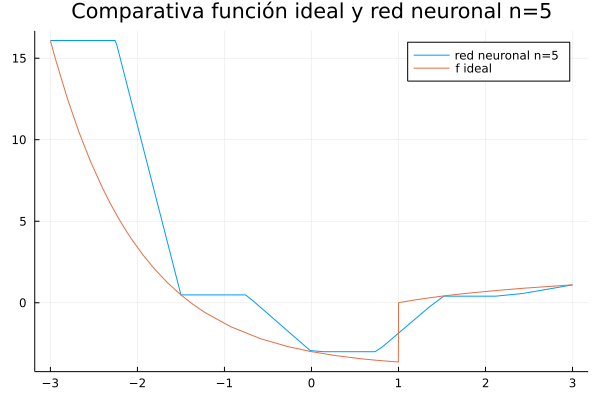
\includegraphics[width=.8\textwidth]{7-algoritmo-inicializar-pesos/f_ideal_y_rn_con_5_neuronas.png}
     \caption{Ejemplo de ejecución del algoritmo de inicialización de pesos}
     \label{img:ch07-ejemplo-5-neuronas-incializacion-pesos}
    \end{figure}




%%%%%%%%%%%%%%%%%%%%%%%%%%%%%%%%%%%%%%%%%%%%%%%%%%%%%%%%%%%%%%%%%%%%
% Experimentación con algoritmo inicialización aprendida DE PESOS
%%%%%%%%%%%%%%%%%%%%%%%%%%%%%%%%%%%%%%%%%%%%%%%%%%%%%%%%%%%%%%%%%%%%

En la siguiente sección trataremos sobre la bondad del algoritmo expuesto

\section{Contraste de hipótesis con inicialización aleatoria} 
\label{ch07:experimento-1} 

Las preguntas a resolver son ¿mejora nuestro algoritmo? ¿Cuánto mejora?

La primera observación  es que como
hemos observado en el modelado de una red neuronal 
en la sección \ref{ch05:construction-evaluation-nnnn}
una red neuronal depende de varios parámetros:
la dimensión de entrada $d$, el número de neuronas en la capa oculta $n$, la dimensión de salida $s$ 
y la funciones de activación de cada neurona.  

Por simplicidad fijaremos una función de activación. 


\subsection{Descripción experimento}

El experimento consta de los siguientes pasos: 

\begin{enumerate}
% Paso 0: Selección de data sets 
\item Dado un conjunto de datos de entrenamiento $\D$  se separará el conjunto en:
\begin{itemize}
    \item $\D_i$ \textbf{Conjunto de 
    datos de entrenamiento e inicialización.} Debe de ser mayor que 
    $n$ y lo suficientemente grande para que el algoritmo diseñado funcione correctamente. 

    \item $\D_t$ \textbf{Conjunto de 
    datos de test.} Se utilizarán para el cálculo del error. 
\end{itemize} 

En particular hemos utilizado el conjunto de datos \href{https://archive.ics.uci.edu/ml/datasets/Airfoil+Self-Noise
    }{
        Airfoil Self-Noise} obtenido del repositorio de datos libres para aprendizaje automático \href{https://archive.ics.uci.edu/ml/datasets.php}{UCI}. 
El conjunto elegido se corresponde a un problema de regresión con $1503$ instancias y $6$ atributos. 
Para la implementación realizada podría utilizarse cualquier otra que provenga de un problema de regresión. 

Notemos que $d$ viene determinado por el número de atributos, 
$s$ será uno ya que estamos frente a un problema 
de regresión de variable real y $n$ vendrá dado como $n = \lfloor \alpha |\mathcal{D}_i| \rfloor$ con $\alpha \in (0,1)$; concretamente, en virtud de la observaciones mostradas en la 
sección \ref{section:inicializar_pesos} de que la probabilidad de 
que un dato no pueda ser utilizado para el algoritmo es nula; 
suponer que el $90\%$ de los datos sí serán válidos es una 
estimación lo suficientemente precavida como para que el algoritmo 
no \textit{falle}, es decir haremos    $\alpha = 0.9$. 

% Paso 1: Construcción 
\item Fijados $n, d$ y $s$ se generarán dos redes neuronales: 

\begin{itemize}
    \item Una inicializada de manera aleatoria con valores dentro de un rango de valores. 
    
    \item  Otra inicializada con nuestro algoritmo, se medirá el $t_i$ tiempo y el error $\varepsilon_i$ en  $\D_t$. 
\end{itemize}

% Paso 2: Evaluación del error
\item Con los datos de entrenamiento $D_i$ y el algoritmo de 
aprendizaje de \textit{backpropagation} se entrenará la red 
neuronal inicializada aleatoriamente hasta que iguale o sea menor que  el 
error del algoritmo de inicialización aprendida $\varepsilon_i$. 

Puesto que puede darse el caso de 
quedar estancados en un mínimo local superior al error encontrado con el algoritmo de inicialización aprendida $\varepsilon_i$ o que oscile entorno a un 
mínimo si el $\eta$ no es lo suficientemente pequeño (ver 
propiedades del gradiente descendente \ref{ch05:gradiente-descentente}); se ha añadido también como criterio de parada el que el error del algoritmo de \textit{backpropagation}
se estanque o empeore durante 5 \footnote{El valor de 5 
iteraciones consecutivas es una heurística observada en 
ejecuciones anteriores y dependiente de $\eta$ y del problema.
Pude observar la traza de de ejecución si ejecuta el experimento.} 
iteraciones consecutivas. 

Durante el experimento se medirá el tiempo que necesita hasta su fin $t_b$ y el error en 
entrenamiento y test. 

Los tiempos $t_i$ y $t_b$ serán los que compararemos con el test de hipótesis. 
\end{enumerate}

Los pasos 2 y 3 se repetirán tantas veces como 
muestras se desee tomar. 

\subsection{Contraste de hipótesis}

Se desea comparar si las diferencias en los tiempos observados efectivamente son notables: 

Para ello se realizará un test de Wilcoxon, con las siguientes hipótesis

\begin{itemize}
    \item $H_0$: La mediana de la diferencia de tiempos  $t_i$ y $t_b$ de cada par de muestras es cero. 
    \item $H_a$: La mediana de las diferencia de tiempos  $t_i$ y $t_b$ entre cada par de muestras es diferente de cero. 
\end{itemize}

La utilidad de este test es que si rechaza la hipótesis nula sabremos que con un $95 \%$ de certeza tendrán medianas diferentes, es decir, \textbf{existe una 
diferencia en los errores}. En caso de que no se rechace no podremos afirmar nada.
Puede encontrar la implementación en el repositorio del
 proyecto \footnote{En el directorio de experimentos 
 de \url{https://github.com/BlancaCC/TFG-Estudio-de-las-redes-neuronales}.}.

\subsection{Requisitos técnicos}  

A la vista de todo el proceso descrito surgen las siguientes necesidades técnicas que deberemos de implementar:  

\subsubsection{Lectura y tratamiento de los datos}

Se necesita ser capaces de leer los datos desde los ficheros descargados, es decir, ser capaces de transformar el formato \textit{.dat} en un \textit{.csv}. 
Además, es necesario un tratamiento previo de los datos: 
\begin{itemize}
    \item Comprobación de que no hay valores nulos o perdidos. 
    \item Normalización de los datos. 
\end{itemize}


\subsubsection{Capacidad de crear una red neuronal aleatoria}  

Deberá de crearse una red neuronal con entradas dentro de un rango $[a,b]$ con $a < b$ reales,
que tenga una entrada de tamaño $d$,
$n$ neuronas en la capa oculta y
una dimensión de salida $d$.

\subsubsection{Implementación del algoritmo de inicialización aprendida}

Deberá implementarse el algoritmo  \ref{algo:algoritmo-iniciar-pesos} con todos los requisitos y atributos que ahí se describe.  

\subsubsection{Función para medir el error}

Deberá implementarse una función para medir el
 error, puesto que nos hayamos frente a un problema de regresión utilizaremos el error cuadrático medio. 

\subsubsection{Forma de evaluar las redes neuronales}  

Dados una red neuronal, una función de evaluación y un vector de atributos de dimensiones adecuadas a la red neuronal debe ser capaz de aplicar el algoritmo de \textit{forward propagation} descrito en \ref{algoritmo:evaluar red neuronal}.

\subsubsection{Implementación del aprendizaje de una red neuronal} 
% Nota en el margen sobre la derivada
\marginpar{\maginLetterSize
    \iconoAclaraciones \textcolor{dark_green}{     
        \textbf{
            Qué es una derivada débil.
        }
    }
    Es una generalización de las derivadas para funciones del espacio $L_p$, esto nos permite
    definir derivadas aunque no lo sea en algunos puntos (recodemos que demostremos el teorema de aproximación universal para estos espacios en la sección \ref{ch04:espacios-Lp}).   
}
Se implementará el algoritmo propio de aprendizaje basado en \textit{backpropagation} y ya optimizado 
que describimos en los algoritmos \ref{algoritmo:gradiente-descendente} y \ref{algoritmo:calculo-gradiente}.
Cabe destacar que para este algoritmo es necesario usar la derivada de las funciones de las funciones de activación. Se ha implementado la derivada débil de ellas. Además se ha seguido el mismo criterio de diseño que ya se tuvo con las funciones de activación en la sección \ref{ch06:activation-function-implementation}.

\subsubsection{Implementación del experimento} 
Deberá implementarse una función que realice el 
experimento tal cual hemos descrito en \ref{ch07:experimento-1}.

\subsection{Resultados obtenidos}

Concretamente de el experimentos se ha realizado con 
una partición del conjunto de datos $\frac{3}{4}|\mathcal{D}|$ para entrenamiento entrenamiento 
y el resto de test. Se ha repetido además $15$ veces (por tratarse de un número conveniente de muestras para el Test de los signos de Wilcoxon como vimos en la sección \ref{ch06:test-hipotesis-propiedades} donde se usó por primera vez). 

Durante cada iteración los datos del conjunto han sido desordenados y el tiempo medido ha sido estrictamente el de creación y aprendizaje de la red neuronal. 

Puede consultar los resultados obtenidos en 
\href{https://github.com/BlancaCC/TFG-Estudio-de-las-redes-neuronales/tree/main/Experimentos/inicializacion-pesos-red-neuronal/resultados/2_air_self_noise}{la carpeta de experimentos de air self noise} 
de nuestro repositorio, es más para obtener
 una información detallada del mismo ejecute 
 los experimentos y observe la información que van mostrando. 


De donde se tiene que para nuestro algoritmo de inicialización aprendida el tiempo medio de ejecución es de 
\begin{equation}
    0,044 \pm 0,064 \text{ segundos, }
\end{equation}
mientras que para la inicialización aleatoria y aprendizaje con el método de 
\textit{backpropagation} es de 
\begin{equation}
    5,284 \pm 0,407   \text{ segundos}.
\end{equation}

Además el test de los signos de Wilcoxon ha rechazado la hipótesis nula
con un $95\%$ de confianza,
por lo que podemos afirmar que efectivamente la diferencia de tiempos es significativa. 

El gráfico de caja bigote con los tiempos es el siguiente: 

\begin{figure}[H]
    \centering
     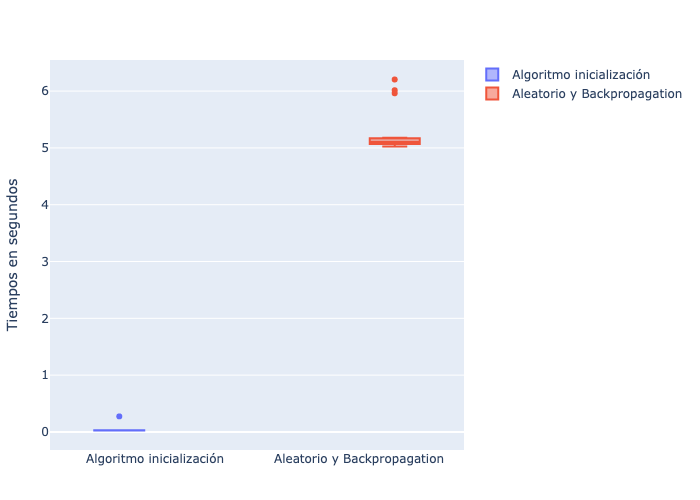
\includegraphics[width=0.8\textwidth]{7-algoritmo-inicializar-pesos/experimento/grafico-bigotes-tiempo.png}
     \caption{Gráfico de caja y bigotes del tiempo requerido por el algoritmo de inicialización aprendida de pesos y el de \textit{backpropagation}.}
\end{figure}
Debemos ser cautos antes de afirmar que tal relación entre los tiempos es el índice de mejora. Puesto que antes debe de conocerse el motivo por el que se detuvo el algoritmo de \textit{backpropagation}; para ello se estudiará la distribución de los errores en entrenamiento. 

\begin{figure}[H]
    \centering
     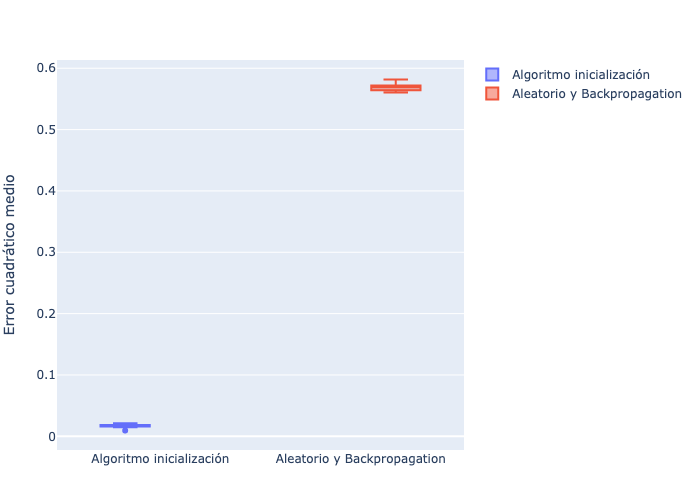
\includegraphics[width=0.8\textwidth]{7-algoritmo-inicializar-pesos/experimento/grafico-bigotes-error_entrenamiento.png}
     \caption{Gráfico de caja y bigotes del \textbf{error en entrenamiento tras finalizar } el algoritmo de inicialización aprendida de pesos y el de \textit{backpropagation}.}
     \label{img07:error-entrenamiento}
\end{figure}

En promedio el error cuadrático medio dentro del entrenamiento conseguido con nuestro algoritmo es 
\begin{equation}
    0,017 \pm 0,003;
\end{equation}
mientras que el de inicialización aleatoria y \textit{backpropagation} es de 
\begin{equation}
    0,569 \pm 0,006. 
\end{equation}
Si además se observa la traza obtenida durante la ejecución (ver repositorio), 
no tarda uno en percatarse de que en la mayoría de las muestras, la parada del algoritmo de
\textit{backpropagation} se está produciendo al \textit{estancarse} el error 
en un mínimo local. 

Esta situación si bien nos previene de poder explicitar un coeficiente de mejora 
entre el algoritmo de inicialización aprendida y \textit{backpropagation} desde 
una red neuronal inicializada aleatoriamente, pone de manifiesto su gran potencial de aprendizaje. 
Es por tanto interesante  comparar el error cuadrático medio obtenido en los datos de test, ya que nos dará una estimación verdadera de la bondad del método.  

El error cuadrático medio de ambos métodos en test es el siguiente: 
\begin{figure}[H]
    \centering
     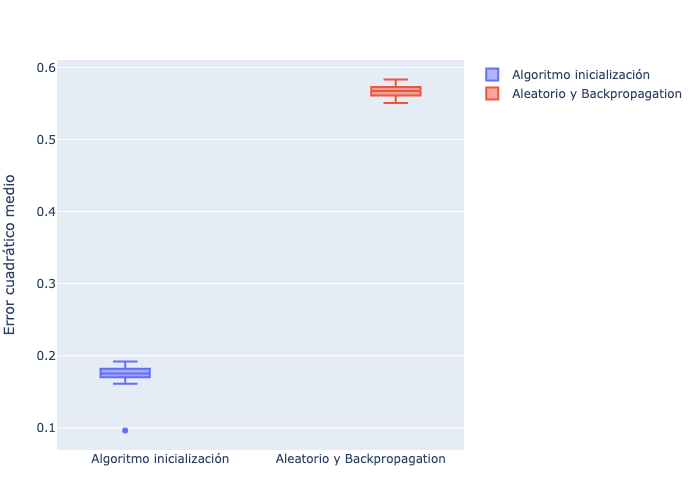
\includegraphics[width=0.8\textwidth]{7-algoritmo-inicializar-pesos/experimento/grafico-bigotes-error_test.png}
     \caption{Gráfico de caja y bigotes del \textbf{error cuadrático medio en test } el algoritmo de inicialización aprendida de pesos y el de \textit{backpropagation}.}
     \label{img07:error-test}
\end{figure}

donde ahora el promedio para nuestro algoritmo de inicialización aprendida es de un error de
\begin{equation}
    0,171 \pm 0,022;
\end{equation}

% Nota sobre sobreajuste 
\marginpar{\maginLetterSize
    \iconoAclaraciones \textcolor{dark_green}{     
        \textbf{
            ¿Qué significa que un modelos está sobreajustado o sobreentrenado?
        }
    }
    En aprendizaje automático un modelo se dice sobreentrenado o sobreajustado 
    cuando ha \textit{aprendido} características 
    propias de los datos de entrenamiento que 
    no son válidas para el problema general. 
    Este efecto produce que se tengan resultados en 
    entrenamiento \textit{considerablemente} mejores que en test.   
}
% fin de la nota
mientras que el de inicialización aleatoria y \textit{backpropagation} es de 
\begin{equation}
    0,567 \pm 0,009.
\end{equation}


A diferencia del error en test obtenido con \textit{backpropagation}, el de nuestro algoritmo
 ha superado al de entrenamiento, lo que indica un sobreajuste 
del modelo a los datos de entrenamiento. Esto es totalmente de esperar por 
cómo se construye la inicialización de pesos. Sin embargo, a pesar del sobreajuste, el resultado sigue siendo mejor tanto en precisión como en tiempo que el de aprendizaje usando \textit{backpropagation}.  


\section{Observaciones y conclusiones sobre el algoritmo de inicialización aprendida de pesos}


Cabe destacar que si bien el algoritmo se ha diseñado para nuestro 
modelo de red neuronal, la idea se puede extender al resto de modelos 
existentes; para ello bastaría seguir la
demostración y plantear el sistema de ecuaciones adecuado que se 
utilizan en la línea 4 del algoritmo \ref{algo:algoritmo-iniciar-pesos}.

Por otro lado, en nuestro caso concreto, el algoritmo
 de inicialización aprendida ha presentado 
 mejores resultados en precisión y tiempo que la 
 alternativa, esta simultaneidad en los 
 beneficios evita cuantificarlos; ya que para 
 tener un coeficiente de mejora o tiempo debería de fijarse un parámetro (las mismas condiciones de observación) y comparar el otro. 

 Como mostramos por el experimento no ha sido 
 posible fijar el error de estudio, ya que 
 \textit{backpropagation} no ha sido capaz de minimizar la red inicializada aleatoriamente 
 hasta tal error. 

 Por otro lado nuestro algoritmo al no ser iterativo tampoco ha podido adaptarse al de 
 \textit{backpropagation}. 

 Si razonáramos fijando el error, la comparación tampoco es posible, ya que si se observan los tiempo de la traza de ejecución (ver experimento en el repositorio), una sola ejecución de nuestro
 algoritmo ya es más rápida que una iteración de 
 \textit{backpropagation}. 

Para futuros trabajos se podría cuantificar la mejora, para ello
proponemos relajar restricciones de \text{backpropagation} con el fin de 
reducir su tiempo de ejecución y así poder compararlos.
 Proponemos para 
ello reducir el tamaño del conjunto de entrenamiento en cada iteración. De esta forma se podría obtener un tiempo por iteración que sea 
divisor del que emplee el algoritmo de inicialización aprendida 
y de esta manera sí poder fijar un tiempo común con el comparar el error. 
\newpage


%%%%%%%%%%%%%%%%%%%%%%%%%%%%%%%%%%%%%%%%%%%%%%%%%%%%
%                 CONCLUSIÓN INTUITIVA 
%      para poder finiquitar la memoria a tiempo
%%%%%%%%%%%%%%%%%%%%%%%%%%%%%%%%%%%%%%%%%%%%%%%%%%%%

\section{Utilidad del algoritmo de inicialización aprendida de pesos en problemas de teoría de la aproximación clásicos}

El algoritmo que acabamos de implementar no solo 
tiene su utilidad en el uso de inicialización de pesos 
de redes neuronales, sino que resuelve problemas 
de teoría de aproximación clásicos. 

Para mostrar esto habrá que remontarse a los ejemplos
del comienzo de este trabajo.  
En la sección \ref{ch03:conclusiones-teoria-aproximacion}
se mostraba que había algunas funciones cuyo error
de aproximación  tendía a infinito.
Gracias al teorema \ref{teo:MFNAUA} sabemos que 
las redes neuronales convergen llevando el error 
a cero. 

Véase cómo se aproxima ahora el ejemplo patológico
que se mostraba en la figura \ref{fig:aproximacion-lagrage}: 

\begin{figure}[H]
    \centering
    \begin{subfigure}[b]{0.475\textwidth}
        \centering
        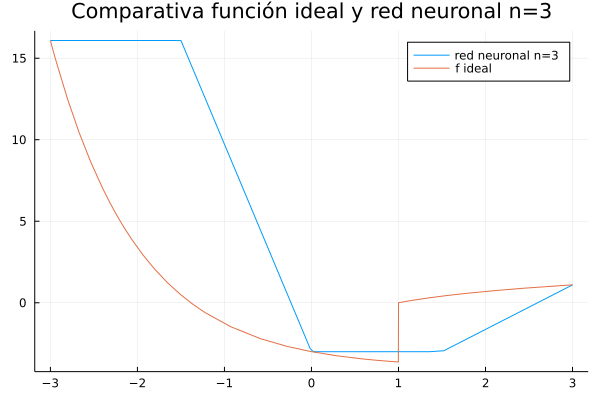
\includegraphics[width=\textwidth]{7-algoritmo-inicializar-pesos/f_ideal_y_rn_con_3_neuronas.png}
        \caption[Network2]%
        {{\small Red neuronal inicializada a partir de 3 datos}}    
    \end{subfigure}
    \hfill
    \begin{subfigure}[b]{0.475\textwidth}  
        \centering 
        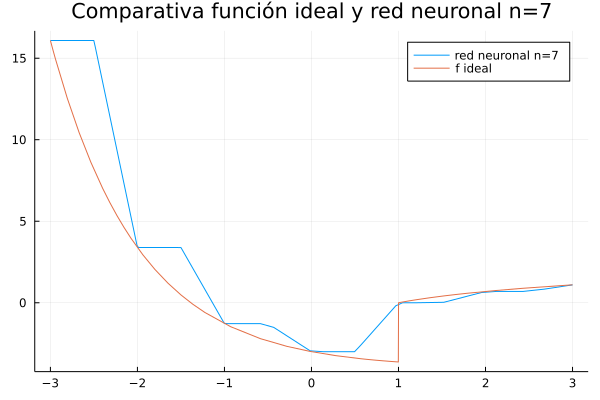
\includegraphics[width=\textwidth]{7-algoritmo-inicializar-pesos/f_ideal_y_rn_con_7_neuronas.png}
        \caption[]%
        {{\small Red neuronal inicializada a partir de 7 datos}}    
    \end{subfigure}
    \vskip\baselineskip
    \begin{subfigure}[b]{0.475\textwidth}   
        \centering 
        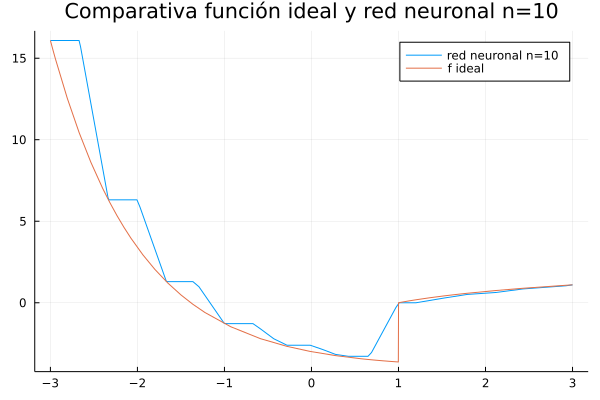
\includegraphics[width=\textwidth]{7-algoritmo-inicializar-pesos/f_ideal_y_rn_con_10_neuronas.png}
        \caption[]%
        {{\small Red neuronal inicializada a partir de 10 datos}}    
    \end{subfigure}
    \hfill
    \begin{subfigure}[b]{0.475\textwidth}   
        \centering 
        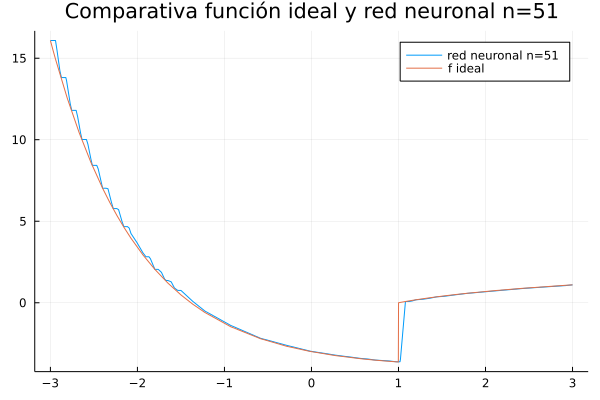
\includegraphics[width=\textwidth]{7-algoritmo-inicializar-pesos/f_ideal_y_rn_con_51_neuronas.png}
        \caption[]%
        {{\small Red neuronal inicializada a partir de 51 neuronas}}    
    \end{subfigure}
    \caption{Ejemplo de aproximación de la función $f(x)$ con redes neuronales.} 
    \label{fig:aproximacion-red-neuronal}
\end{figure}
\begin{figure}[H]
    \centering
     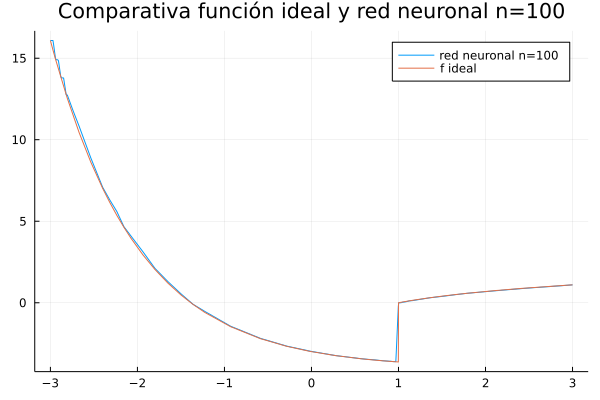
\includegraphics[width=.5\textwidth]{7-algoritmo-inicializar-pesos/f_ideal_y_rn_con_100_neuronas.png}
     \caption{Ejemplo de aproximación de la función $f(x)$ con red neuronal de 100 neuronas.}
     \label{fig:aproximacion-red-neuronal-2}
    \end{figure}

% Comentario sobre los algoritmos genéticos 
%%%%%%%%%%%%%%%%%%%%%%%%%%%%%%%%%%%%%%%%%%%%%%%%
%    Combinación de distintas funciones 
%              de activación 
%%%%%%%%%%%%%%%%%%%%%%%%%%%%%%%%%%%%%%%%%%%%%%%%
\newpage
\chapter{Futuros trabajos: Selección genética de las funciones de activación }
\label{ch08:genetic-selection}

Como se indicó en \ref{ch03:funcionamiento-intuitivo-funcion-activacion}
aunque la convergencia universal no 
dependa de la función de activación seleccionada,
fijado cierto número de neuronas, éstas sí que pueden 
determinar el error mínimo que podamos alcanzar.  

Gracias al resultado \ref{cor:se-generaliza-G-a-una-familia} es posible combinar en una red neuronal distintas funciones de activación y que el teorema de convergencia universal \ref{teo:MFNAUA} se mantenga cierto, esto abre la puerta a explorar también durante el entrenamiento diferentes funciones de activación. De hecho ya existen artículos como \cite{FunctionOptimizationwithGeneticAlgorithms} y \cite{Genetic-deep-neural-networks} donde se desarrolla de manera experimental esta idea. 

El problema que se tiene es que al aumentar
el número de funciones de activación candidatas, se está aumentando también el espacio de búsqueda; lo que significa que la complejidad del espacio aumenta y por ende el coste para encontrar una solución. 

Se ha intentado paliar la situación con algoritmos genéticos (véanse los artículos recién citados). Sin embargo, existen dos detalles claves y novedosos que podemos aportar: el primero es que \textbf{con nuestro teorema \ref{teo:eficacia-funciones-activation}}  se ha obtenido un 
criterio de selección de las funciones de activación que 
tendrán el mismo potencial de aproximación y menor coste; 
esto \textbf{nos ahorraría tener que explorar combinaciones de 
funciones de activación que no vaya a aportar en precisión y 
además aumenten el costo.} 


El segundo reside en que en los artículos que versan sobre el tema, 
utilizan modelos de \textit{deep learning} sensibles a la posiciones de las función de activación. Es decir, que para $n$ neuronas y $t$ funciones de activación diferentes el tamaño del espacio de búsqueda es $t^n$. Sin embargo, una de las ventajas que presenta \textbf{nuestro modelo} es que \textbf{es invariante ante cambios de posición de funciones de activación;} por lo que una vez fijado el número de cada tipo de funciones de activación da igual la neurona dónde se posicionen (esto es fácil de comprobar observando el modelo \ref{chapter:construir-redes-neuronales} y por la propiedad conmutativa de la suma).

Es decir, \textbf{con nuestro modelo y resultados se estaría reduciendo el espacio de búsqueda y por tanto merecería la pena plantearse de nuevo este tipo de experimentos}. 


%% !TeX root = ../../tfg.tex
% !TeX encoding = utf8
%
%*******************************************************
% Hipótesis planteadas 
%*******************************************************

\chapter{Hipótesis de optimización }
\textcolor{red}{ATENCIÓN: Todos este capítulo está como notas personales}

\section{A qué nos referimos con optimización}
ES necesario decir qué queremos optimizar
Ejemplo: 
- Mejores resultados para mismo tiempo. 

Medir error y tiempo de cálculo. 

Es por ello que es necesario establecer cómo lo vamos a medir.



\textcolor{red}{ATENCIÓN: Todo este capítulo está como notas personales}  


En esta sección recopilaremos las posibles ideas que podrían optimizar las 
redes neuronales, describiremos una experimentación para contrastar los resultados y mostraremos sus conclusiones. 

\section{Democratización de la función de activación}\label{hypothesis:activation-function}

La primera pregunta, existe alguna función de activación 
claramente mejor en algún sentido que las otras. 

Haciendo un estudio computacional de evaluaciones concretas sí. 
(TODO: hacer experimento)

Pero eso no significaría que fuera mejor para
evaluar los resultados en una red neuronal real. 
(hacer experimento)

Este experimento depende de los datos y da lugar a la siguiente pregunta. 

¿Existe una dependencia en la mejora de los resultados 
con respecto de los datos?

Es decir si tenemos dos redes neuronales $f$ y $g$  de mismo número de neuronas y distintas funciones de activación y dos conjuntos de entrenamiento $D_1$, $D_2$

¿Podría darse el caso de que para $D_1$ $f$ aprenda mejor pero que para $D_2$ $g$ sea mejor?. 


Vamos a tratar de encontrar de encontrar un ejemplo de esto.

\section{Inicialización de la pesos red neuronal}\label{hypothesis:pesos-iniciales}

\section{Construcción dinámica del número de neuronas}



%%%%%%%%%%%%%%%%%%%%%%%%%%%%%%%%%%%%%%%%%%%%%%%%%%%%
% Conclusiones del trabajo
%%%%%%%%%%%%%%%%%%%%%%%%%%%%%%%%%%%%%%%%%%%%%%%%%%%%

\chapter{Conclusiones} 
\label{ch09:conclusion}
Era nuestro objetivo con este trabajo esclarecer 
el motivo y funcionamiento de las redes neuronales y 
a partir de ahí optimizar algún aspecto de ellas. 

El sustento teórico queda expuesto en los capítulos 
\ref{ch00:methodology}, \ref{chapter:Introduction-neuronal-networks},
\ref{ch03:teoria-aproximar}, \ref{chapter4:redes-neuronales-aproximador-universal}
y \ref{chapter:construir-redes-neuronales}. 
Hemos contribuido al estado del arte actual con los 
resultados: 

\begin{itemize}
    \item La propuesta del uso de modelo de red neuronal (definición \ref{img:grafo-red-neuronal-una-capa-oculta}).
    \item La demostración teórica del uso de distintas funciones de activación en 
    el modelo seleccionado (corolario \ref{cor:se-generaliza-G-a-una-familia}). 
    \item La demostración de la densidad del espacio de las redes neuronales racionales en el espacio de las funciones medibles (teorema \ref{teo:densidad-racional}).
    \item Resultados sobre la irrelevancia del sesgo en las redes neuronales (sección \ref{consideration-irrelevancia-sesgo}).
    \item Una alternativa al uso de funciones de clasificación (sección \ref{ch05:dominio-discreto}).
    \item Un criterio de selección de funciones de activación (capítulo \ref{funciones-activacion-democraticas-mas-demoscraticas}).
    \item Resultados teóricos sobre la equivalencia de funciones de activación (teorema \ref{teo:equivalencia-grafos-activation-function} y 
    corolario \ref{corolario:afine-activation-function}).
    \item Un algoritmo de inicialización aprendida de los pesos de una red neuronal que acelera los métodos de aprendizaje iterativos (capítulo \ref{section:inicializar_pesos}).
    \item La biblioteca \textit{OptimizedNeuralNetwork.jl} que aporta un modelo y métodos optimizados para el uso de redes neuronales. 
\end{itemize}

y proponemos como posibles vías de investigación en proyectos futuros: 

\begin{itemize}
    \item Una revisión de la selección genética de funciones de activación con nuestro modelo (capítulo \ref{ch08:genetic-selection}).
    \item Una investigación sobre la repercusión en la convergencia de la delimitación de la precisión en los coeficientes de las redes neuronales (sección \ref{ch04:capacidad-calculo}). 
\end{itemize}

Pero finalmente y sobretodo, me llevo la grata experiencia de 
todo el proceso que ha conllevado este Trabajo Fin de Grado;
con las habilidades de gestión bibliográfica, comprensión y expresión rigurosa que ello implica;
así como el método adquirido, constancia y paciencia;
y por supuesto la satisfacción personal de haber sido capaz de acabar un proyecto 
de estas características. 




% --------------------------------------------------------------------
% APPENDIX: Opcional
% --------------------------------------------------------------------

\appendix % Reinicia la numeración de los capítulos y usa letras para numerarlos
\pdfbookmark[-1]{Apéndices}{appendix} % Alternativamente podemos agrupar los apéndices con un nuevo \part{Apéndices}


%% !TeX root = ../libro.tex
% !TeX encoding = utf8

\chapter{Documentación}\label{ap:documentacion}

En este apéndice se deja la documentación en estilo \emph{python} de la documentación de las distintas clases, métodos y funciones más importantes implementados en el proyecto.

\section{Selección de Modelos}

Las clases implementadas para la parte de selección de modelos que se pueden encontrar en la carpeta $PV/src$.

\subsection{Perturbated Validation}

Esta clase y sus métodos se encuentran en el archivo $PV.py$.

\paragraph{PV}

Clase PV que implementa el método para calcular y manejar la heurística PV. Guarda los datos de las series originales, las perturbaciones realizadas, los ratio de error, el nombre del dataset que se está perturbando, y valores auxiliares para imprimir gráficas del cálculo del PV.

\begin{lstlisting}
class PV:
    """
        Clase que implementa Perturbation Validation (PV).

        Attributes
        ----------
        X : np.array
            Dataset
        y : np.array
            Conjuto de etiquetas perturbadas
        ds_name : str
            Nombre del dataset
        errs : np.array
            Errores tomados
        counter : int
            Contador auxiliar
        fig : Figure
            Figura actual
        ax : Axes
            Ejes actuales
    """
\end{lstlisting}

\paragraph{Constructor}

Constructor de la clase PV que necesita los datos originales, el número de perturbaciones, el nombre del \emph{dataset}, y el inicio y fin de los ratio de error. Crea los conjuntos de etiquetas perturbadas.

\begin{lstlisting}
def __init__(self, X, y, n_pv = 5, ds_name = "", err_ini = 0.1,
                 err_fin = 0.3):
        """
            Inicializa la clase creando las etiquetas perturbadas.

            Las perturbaciones se realizan tomando un %err de cada
            clase, poniendole otra etiqueta distinta.

            Se toman "n_pv" puntos entre [err_ini, err_fin].

            Parameters
            ----------
            X : np.array
                Dataset
            y : np.array
                Etiquetas
            n_pv: int
                Número de puntos/errores
            ds_name: str
                Nombre del datases
            err_ini : float
                Error inicial
            err_fin : float
                Error final
        """
\end{lstlisting}

\paragraph{Cálculo PV}

Método para calcular el valor PV de un modelo dado.

\begin{lstlisting}
def get_pv(self, clf, clf_name = "", plot = True):
        """
            Calcula el PV score para el clasificador.

            Parameters
            ----------
            clf : Classifier
                Clasificador
            clf_name : str
                Nombre del clasificador

            Returns
            -------
            pv : float
                PV score
            accs : list(float)
                accs obtenidos
        """
\end{lstlisting}

\paragraph{Dibujar cálculo PV}

Método para representar en una gráfica los valores de la métrica $acc$ obtenidos en el cálculo de PV junto a la recta de regresión obtenida.

\begin{lstlisting}
def plot_pv(self, errs, accs, poly, pv, clf_name = ""):
        """
            Dibuja los puntos y la recta de regresión en la figura actual.

            Parameters
            ----------
            errs : np.array
                Errores
            accs : np.array
                acc obtenidos
            poly : np.array
                Recta de regresión
            pv : float
                Valor PV
            clf_name : str
                Nombre del clasificador
        """
\end{lstlisting}

\paragraph{Guardar gráfica}

Método para guardar en una imagen .png el gráfico del método $plot\_pv$.

\begin{lstlisting}
def save_graph(self, name_fig):
        """
            Guarda el gráfico de los resultados en un .png

            Parameters
            ----------
            name_fig : str
                Nombre (ruta) de la imagen a guardar.
        """
\end{lstlisting}

\subsection{Clasificador LSTM}

Esta clase y sus métodos se encuentran en el archivo $LSTM.py$.

\paragraph{LSTM}

La clase LSTM que implementa el clasificador LSTM. Guarda el modelo LSTM, el número de clases, la longitud de las series, opciones de entrenamiento y para gráficas de entrenamiento.

\begin{lstlisting}
class LSTM(BaseEstimator):
    """
        Implementación de una red neuronal con capas LSTM.

        Attributes
        ----------
        counter : int, static
            Valor auxiliar para ruta de imagen
        model : Sequential
            Modelo red neuronal
        history : list
            Historial del entrenamiento
        n_clases : int
            Número de clases de las etiquetas
        input_shape : tuple
            Forma de los datos
        epochs: int
            Número de épocas para entrenamiento
        verbose : int
            Información sobre el entrenamiento
        save_hist : boolean
            Si guardar las gráficas de los entrenamientos
    """
\end{lstlisting}

\paragraph{Constructor}

Constructor de la clase LSTM que guarda opciones de entrenamiento.

\begin{lstlisting}
def __init__(self, epochs, n_neurs = 80, verbose = 0, save_hist = False,
             n_clases = -1):
        """
            Inicializamos la red LSTM.

            Attributes
            ----------
            epochs : int
                Número de épocas para entrenamiento
            n_neurs : int
                Número de neuronas LSTM
            verbose : int
                Información sobre el entrenamiento
            save_hist : boolean
                Si guardar las gráficas de los entrenamientos
            n_clases : int
                Número de clases a predecir
        """
\end{lstlisting}

\paragraph{Creación del modelo}

Método para crear el modelo LSTM.

\begin{lstlisting}
def create_model(self):
        """
            Crea el modelo LSTM.
        """
\end{lstlisting}

\paragraph{Compilar el modelo}

Compila el modelo con el optimizador ADAM y la función de pérdida entropía cruzada categórica.

\begin{lstlisting}
def compile_model(self):
        """
            Compila el modelo con optimizador ADAM y función de pérdida
            categorical_crossentropy.
        """
\end{lstlisting}

\paragraph{Entrenamiento}

Método para entrenar el modelo con el conjunto de datos, con las épocas guardadas, validación al 10\% y con parada temprana.

\begin{lstlisting}
def fit(self, X, y):
        """
            Entrenamos el modelo.

            Parameters
            ----------
            X : numpy.array
                Datos de entrenamiento
            y : numpy.array
                Etiquetas de entrenamiento
        """
\end{lstlisting}

\paragraph{Cálculo métrica}

Método para calcular la métrica $acc$ en el conjunto de datos pasado.

\begin{lstlisting}
def score(self, X, y):
        """
            Calcula el acc con los datos que se le pasan.

            Parameters
            ----------
            X : numpy.array
                Datos test
            y : numpy.array
                Etiquetas test

            Returns
            ----------
            acc : float
                accuracy obtenida
        """
\end{lstlisting}

\paragraph{Guardar gráfica de entrenamiento}

Método para guardar el historial de entrenamiento en una imagen.

\begin{lstlisting}
def save_history(self):
        """
            Guarda el historial en una imagen.
        """
\end{lstlisting}

\subsection{Clasificadores}

Los clasificadores adicionales que usamos para comparar modelos, comparten dos métodos generales: entrenamiento y cálculo de la métrica.

\paragraph{Entrenamiento}

Método que se encarga de entrenar el modelo usando una muestra de datos.

\begin{lstlisting}
def fit(self, X, y):
    """
        Entrena el modelo.

        Parameters
        ----------
        X : numpy.array
            Datos de entrenamiento
        y : numpy.array
            Etiquetas de entrenamiento
    """
\end{lstlisting}

\subparagraph{Cálculo de métrica}

Método que se encarga de calcular la métrica ($accuracy$) de un modelo en un conjunto de datos.

\begin{lstlisting}
def score(self, X, y):
    """
        Calcula el acc con los datos que se le pasan.

        Parameters
        ----------
        X : numpy.array
            Datos test
        y : numpy.array
            Etiquetas test

        Returns
        ----------
        acc : float
            accuracy obtenida
    """
\end{lstlisting}

\subsubsection{C4.5}

Esta clase y sus métodos se encuentran en el archivo $RClassifiers.py$.

\paragraph{C45}

La clase C45 que usa el árbol de decisión C4.5 que guarda el modelo.

\begin{lstlisting}
class C45(BaseEstimator):
    """
        Implementa el árbol de decisión C4.5.

        Attributes
        ----------
        model : clasificador en R
            El clasificador (clase en R)
    """
\end{lstlisting}

\subsubsection{C5.0}

Esta clase y sus métodos se encuentran en el archivo $RClassifiers.py$.

\paragraph{C50}

La clase C50 que usa el árbol de decisión C5.0 que guarda el modelo, y también el valor del \emph{boosting}.

\begin{lstlisting}
class C50(BaseEstimator):
    """
        Implementa el árbol de decisión C5.0 (con boosting o no).

        Attributes
        ----------
        model : clasificador en R
            El clasificador (clase en R)
        boosting : int
            El valor del boosting
    """
\end{lstlisting}

\paragraph{Constructor}

Constructor de la clase C50 que se le pasa el número de \emph{boosting} que se necesite.

\begin{lstlisting}
def __init__(self, boosting = 10):
        """
            Inicializa el clasificador.

            Parameters
            ----------
            boosting : int
                El valor del boosting
        """
\end{lstlisting}

\subsubsection{Recursive Partioning Tree}

Esta clase y sus métodos se encuentran en el archivo $RClassifiers.py$.

\paragraph{RPart}

Clase que usa el árbol RPart.

\begin{lstlisting}
class RPart(BaseEstimator):
    """
        Implementa el árbol de decisión RPart (Recursive Partioning Tree).

        Attributes
        ----------
        model : clasificador en R
            El clasificador (clase en R)
    """
\end{lstlisting}

\subsubsection{Condicional Tree}

Esta clase y sus métodos se encuentran en el archivo $RClassifiers.py$.

\paragraph{CTree}

La clase CTree implementa el uso del árbol de decisión Condicional Tree.

\begin{lstlisting}
class CTree(BaseEstimator):
    """
        Implementa el árbol de decisión CTree (Conditional Inference Tree).

        Attributes
        ----------
        model : clasificador en R
            El clasificador (clase en R)
    """
\end{lstlisting}


\subsubsection{$k$-NN}

Esta clase y sus métodos se encuentran en el archivo $KNN.py$.


\paragraph{Clase KNN}

Clase que implementa el clasificador $k$-NN que se le puede pasar el $k$ fijo o que lo calcule automáticamente tomado como la raíz cuadrada del número de datos.

\begin{lstlisting}
class KNN(BaseEstimator):
    """
        Implementa el clasificador KNN (K-Nearest neighbors).

        Parameters
        ----------
        k : int
            Número de vecinos
        model : KNeighborsClassifier
            Modelo k-NN
        metric : str, metric
            Métrica que usar con KNN
        n_jobs : int
            Número de procesadores usados
    """
\end{lstlisting}

\paragraph{Constructor}

Constructor de la clase KNN que necesita el número de vecinos, la métrica y el número de procesadores.

\begin{lstlisting}
def __init__(self, k = None, metric = "euclidean", n_jobs = 1):
        """
            Inicializa el clasificador.

            Parameters
            ----------
            k : int
                Número de vecinos
            metric : str, metric
                Métrica que usar con KNN
            n_jobs : int
                Número de procesadores
        """
\end{lstlisting}

\subsubsection{$k$-NN + DTW}

Esta clase y sus métodos se encuentran en el archivo $RClassifiers.py$.

\paragraph{DTW}

Clase que implementa el clasificador $k$-NN con métrica DTW, que guarda los datos de entrenamiento, el número de vecinos y el tamaño de la ventana para aplicar DTW.

\begin{lstlisting}
class DTW(BaseEstimator):
    """
        Clase que implementa K-Nearest Neighbors con la distancia DTW
        usando la implementación del paquete "IncDTW".

        Attributes
        ----------
        data : R.DataFrame
            Datos transformados en un objeto dataframe de R
        k : int
            Número de vecinos
        window_shift : int
            Tamaño de la ventana para aplicar DTW
    """
\end{lstlisting}

\paragraph{Constructor}

Constructor de la clase DTW que necesita el número de vecinos y el tamaño de la ventana para el cálculo de la métrica DTW.

\begin{lstlisting}
def __init__(self, k = 1, window_shift = 5):
    """
        Constructor de la clase, debe hacerse solo una vez por dataset.

        Parameters
        ----------
        k : int
            Números de vecinos
        window_shift : int
            Tamaño de la ventana para aplicar DTW
    """
\end{lstlisting}

\section{Detección de anomalías}

Funciones y clases relativas a la parte de detección de anomalías que se encuentran en la carpeta $AD/src$.

\subsection{Alteración de series}

Funciones para la creación de anomalías en base a las series normales implementadas en el archivo $alteraciones.py$.

\paragraph{Tramo aleatorio}

Función para escoger un tramo aleatorio de la serie en función a la longitud indicada (máxima, mínima, fija).

\begin{lstlisting}
def random_slice(x, max_length = None, min_length = None,
                   length = None, pos = None, border = 0):
    """
        Se encarga de elegir un tramo aleatorio de una serie que queda
        determinado por una posición y longitud, de manera que el tramo
        elegido es [posición, posición + longitud).

        Se puede determinar una longitud máxima o mínima, o incluso
        especificar una longitud o posición fijada. También se puede
        indicar si excluir los extremos (añadir borde).

        Parameters
        ----------
        x : np.numpy
            Serie temporal que alterar
        max_length : int, None
            Longitud máxima de la perturbación
        min_length : int, None
            Longitud mínima de la perturbación
        length : int, None
            Longitud fija de la perturbación
        pos : int, None
            Posición fija de la perturbación
        border : int
            Borde para excluir la perturbación

        Returns
        -------
        pos : int
            Posición de la perturbación
        length : int
            Longitud de la perturbación
    """
\end{lstlisting}

\paragraph{Ruido gaussiano}

Método para alterar un tramo aleatorio de la serie añadiendo ruido gaussiano mediante un parámetro $\sigma$ que controla la intensidad de esta perturbación, y la longitud máxima y mínima de esta.

\begin{lstlisting}
def gaussian_noise(x, max_length, min_length = 3, std = 3, neg = False,
                   border = 0, neg_random = True):
    """
        Crea una perturbación de ruido gaussiano añadiendo en un
        tramo aleatorio un muestreo de la función de densidad normal.
        Se puede controlar la intensidad.

        Además se puede activar aleatoriamente (50%) o de manera fija que la
        alteración gaussiana sea negativa.

        Parameters
        ----------
        x : np.numpy
            La serie para alterar
        max_length : int
            Longitud máxima de la alteración
        min_length : int
            Longitud minima de la alteración
        std : float
            Controla la intensidad de la alteración
        neg : boolean
            Si invertir la señal gaussiana
        border : int
            El borde para excluir la perturbación
        neg_random : boolean
            Si se invierte aleatoriamente las señales

        Returns
        -------
        x : np.numpy
            Una copia de la señal perturbada
    """
\end{lstlisting}

\paragraph{Pulso sinusoidal-gaussiano}

Método para alterar un tramo aleatorio de la serie añadiendo un pulso sinusoidal-gaussiano mediante su frecuencia $fc$, un parámetro $\sigma$ que controla la intensidad de la perturbación y la longitud máxima y mínima de esta.

\begin{lstlisting}
def gaussian_sine_pulse(x, max_length, min_length = 3, fc = 1.5, std = 3,
                        border = 0):
    """
        Crea una perturbación con un pulso sinusoidal-gaussiano añadido en un
        tramo aleatorio. Se puede controlar la intensidad y la frecuencia
        del pulso.

        Parameters
        ----------
        x : np.numpy
            La serie para alterar
        max_length : int
            Longitud máxima de la alteración
        min_length : int
            Longitud minima de la alteración
        fc : float
            Frecuencia de la señal del pulso
        std : float
            Controla la intensidad de la alteración
        border : int
            El borde para excluir la perturbación

        Returns
        -------
        x : np.numpy
            Una copia de la señal perturbada
    """
\end{lstlisting}

\paragraph{Estacionalidad}

Método para alterar un tramo aleatorio de la serie modificando la estacionalidad de la descomposición STL (dada con un periodo) por un parámetro $\sigma$ que controla la intensidad y la longitud máxima y mínima de esta.

\begin{lstlisting}
def modify_season(x, period, max_length, min_length = 3, std = 1, border = 0):
    """
        Crea una perturbación multiplicando por un real la estacionalidad
        de un tramo aleatorio de la serie. Se necesita el periodo para
        realizar la descomposición STL.

        Parameters
        ----------
        x : np.numpy
            La serie para alterar
        period : int
            Periodo de repetición de la serie para descomposición STL
        max_length : int
            Longitud máxima de la alteración
        min_length : int
            Longitud minima de la alteración
        std : float
            Controla la intensidad de la alteración
        border : int
            El borde para excluir la perturbación
    """
\end{lstlisting}

\paragraph{Tendencia}

Método para alterar un tramo aleatorio de la serie modificando la tendencia de la descomposición STL (dada con un periodo) por un parámetro $\sigma$ que controla la intensidad y la longitud máxima y mínima de esta.

\begin{lstlisting}
def modify_trend(x, period, max_length, min_length = 3, std = 1, border = 0):
    """
        Crea una perturbación multiplicando por un real la tendencia
        de un tramo aleatorio de la serie. Se necesita el periodo para
        realizar la descomposición STL.

        Parameters
        ----------
        x : np.numpy
            La serie para alterar
        period : int
            Periodo de repetición de la serie para descomposición STL
        max_length : int
            Longitud máxima de la alteración
        min_length : int
            Longitud minima de la alteración
        std : float
            Controla la intensidad de la alteración
        border : int
            El borde para excluir la perturbación
    """
\end{lstlisting}

\subsection{Detector}

Clase y sus métodos implementados para crear el detector de anomalías, implementado en $detector.py$

\paragraph{Clase LSTM\_AD}

Clase que implementa el detector de anomalías basado en autoencoder LSTM. Mantiene el modelo LSTM, la probabilidad estimada y otros parámetros de entrenamiento.

\begin{lstlisting}
class LSTM_AD:
    """
        Clase que implementa un detector de anomalías usando
        un modelo autoencoder con capas LSTM.

        Attributes
        ----------
        model : keras.Sequential
            Autoencoder LSTM
        n_neur : int
            Número de neuronas base para las capas
        alpha : float
            Parámetro de regularización L2
        lr : float
            Learning rate
        epochs : int
            Número de épocas de entrenamiento
        mode : int
            Si incluir espacio de codificación (1) o no (2)
        hist : keras.Historial
            Historial de entrenamiento
        kernel : scipy.gaussian_kde
            Distribución de errores estimada
    """
\end{lstlisting}

\paragraph{Constructor}

Constructor de la clase LSTM\_AD que guarda los parámetros relativos al entrenamiento y al modo de arquitectura.

\begin{lstlisting}
def __init__(self, n_neur = 32, alpha = 0, lr = 0.001, epochs = 300,
             mode = 2):
    """
        Constructor de la clase

        Parameters
        ----------
        n_neur : int
            Número de neuronas base para las capas
        alpha : float
            Parámetro de regularización L2
        lr : float
            Learning rate
        epochs : int
            Número de épocas de entrenamiento
        mode : int
            Si incluir espacio de codificación (1) o no (2)
    """
\end{lstlisting}

\paragraph{Creación del modelo}

Función para crear la arquitectura del modelo autoencoder LSTM.

\begin{lstlisting}
def create_model(self, X):
    """
        Crea la arquitectura del autoencoder LSTM con los atributos
        de la clase.

        Parameters
        ----------
        X : np.numpy
            Series temporales
    """
\end{lstlisting}

\paragraph{Compilación}

Función para compilar el modelo autoencoder LSTM.

\begin{lstlisting}
def compile_model(self):
    """
        Compila el modelo con ADAM añadiendo un clip de 1, learning
        rate especificado y minimizando el error cuadrático medio.
    """
\end{lstlisting}

\paragraph{Entrenamiento}

Función para entrenar el modelo autoencoder LSTM.

\begin{lstlisting}
def load_model(self, path):
    """
        Carga el modelo de unos pesos guardados en un archivo

        Parameters
        ----------
        path : str
            Ruta donde está el archivo de los pesos
    """
\end{lstlisting}

\paragraph{Reconstrucción}

Función para obtener las reconstrucciones de un conjunto de series temporales.

\begin{lstlisting}
"""
    Obtiene las reconstrucciones del autoencoder para las series.

    Parameters
    ----------
    X : numpy.array
        Datasets de series temporales

    Returns
    -------
    reconstrucciones : numpy.array
        Reconstrucciones de las series temporales
"""
\end{lstlisting}

\paragraph{Estimar distribución}

Función para estimar la distribución de los errores de reconstrucción.

\begin{lstlisting}
def fit_kernel(self, X):
    """
        Ajustamos la distribución de los errores de reconstrucción
        con los datos de entrenamiento.

        Parameters
        ----------
        X : numpy.array
            Dataset de series temporales
    """
\end{lstlisting}

\paragraph{Calcular probabilidades}

Función para obtener las probabilidades de ser serie anómala para un conjunto de series temporales.

\begin{lstlisting}
def predict_prob(self, X):
    """
        Devolvemos las probabilidades de ser serie anómala para
        cada serie del dataset

        Parameters
        ----------
        X : numpy.array
            Dataset de series temporales

        Returns
        -------
        probs : numpy.array
            Probabilidades de anomalía para cada serie
    """
\end{lstlisting}

\subsection{Cálculo Curva Precision-Recall}

Las funciones para calcular la métrica $AUC$-$PR$ (curva precisión-recall) que se encuentran en el archivo $calc\_pr.py$.

\paragraph{Contar anomalías}

Se cuentan el número de anomalías detectadas en función de las probabilidades de las series de ser anómalas y de un umbral de probabilidad al partir del cual se considera que es anómala.

\begin{lstlisting}
def count_anomalies(probs, threshold):
    """
        Cuenta cuantas anomalías hay en función a la probabilidad de serlo
        y un umbral de probabilidad.

        Parameters
        ----------
        probs : np.numpy
            Array con probabilidades de cada serie de ser anómala
        threshold : float
            Umbral de probabilidad a partir del cual se considera anómala

        Returns
        -------
        n_anomalies : int
            Número de anomalías detectadas
    """
\end{lstlisting}

\paragraph{Calcular sensibilidad}

Se calcula la sensibilidad del modelo en base a las probabilidades de las series anómalas y un umbral.

\begin{lstlisting}
def calc_recall(probs_anomalies, threshold):
    """
        Calcula la sensibilidad (recall) de un modelo en base a las
        probabilidades de las series anómalas.

        Parameters
        ----------
        probs_anomalies : np.numpy
            Array con probabilidades de anomalías de las series anómalas
        threshold : float
            Umbral de probabilidad

        Returns
        -------
        recall : float
            Sensibilidad del modelo
    """
\end{lstlisting}

\paragraph{Calcular precisión}

Se calcula la precisión del modelo en base a las probabilidades de las series anómalas y normales junto a un umbral.

\begin{lstlisting}
def calc_precision(probs_normal, probs_anomalies, threshold):
    """
        Calcula la precisión de un modelo en base a las probabilidades
        de las series anómalas y normales.

        Parameters
        ----------
        probs_normal : np.numpy
            Array con probabilidades anomalías de las series normales
        probs_anomalies : np.numpy
            Array con probabilidades anomalías de las series anómalas
        threshold : float
            Umbral de probabilidad

        Returns
        -------
        precision : float
            Precisión del modelo
    """
\end{lstlisting}

\paragraph{Curva Precision-Recall}

Se calcula la métrica $PR$ tomando el área debajo de la curva Precision-Recall integrando en el cuadrado $[0, 1]^2$. Además se imprime una figura mostrando la curva que se forma.

\begin{lstlisting}
def recall_precision_curve(X_normal, X_anomalies, model, clf_name = "clf",
                           title = "recall-precision curve", axis = None,
                           plot = True):
    """
        Calcula la métrica PR y además muestra la curva Precision-Recall
        del modelo.

        Parameters
        ----------
        X_normal : np.numpy
            Series normales
        X_anomalies : np.numpy
            Series anómalas
        model : detector
            Detector de anomalías
        clf_name : str
            Nombre del detector
        title : str
            Título de la gráfica
        axis : matplotlib.axis
            Objeto para imprimir las gráficas
        plot : boolean
            Si imprimir cosas opcionales de la gráfica

        Returns
        -------
        pr_score : float
            Valor de la métrica PR
    """
\end{lstlisting}


\endinput
%------------------------------------------------------------------------------------
% FIN DEL APÉNDICE.
%------------------------------------------------------------------------------------


% Añadir tantos apéndices como sea necesario

% --------------------------------------------------------------------
% GLOSARIO: Opcional
% --------------------------------------------------------------------

%\include{glosario}


% -------------------------------------------------------------------
% BACKMATTER
% -------------------------------------------------------------------

\backmatter % Desactiva la numeración de los capítulos
\pdfbookmark[-1]{Referencias}{BM-Referencias}

% BIBLIOGRAFÍA
%-------------------------------------------------------------------

\setbibpreamble{Las referencias se listan por orden alfabético. Aquellas referencias con más de un autor están ordenadas de acuerdo con el primer autor.\par\bigskip}
\bibliographystyle{alphaurl}
\begin{small} % Normalmente la bibliografía se imprime en un tamaño de letra más pequeño.
\bibliography{library.bib}
\end{small}


% ÍNDICE TERMINOLÓGICO  (Opcional)
%-------------------------------------------------------------------

\cleardoublepage
\begin{footnotesize} % Normalmente el índice se imprime en un tamaño de letra más pequeño.
\printindex
\end{footnotesize}
\end{document}
